%======================================================================
%  Nonlinear Problems in Mechanics -- Lecture notes
%  A. Constantinescu, LMS, CNRS & Ecole Polytechnique
%
%  Build:  pdflatex main (three passes; no BibTeX needed -- each
%          chapter carries its own bibliography). The index is built by
%          makeindex, called automatically by imakeidx (or use latexmk).
%  Work on one chapter: uncomment the \includeonly line.
%======================================================================
\documentclass[11pt,a4paper,twoside,openright]{book}

%======================================================================
%  style.tex -- page layout and typography
%  Visual language taken from the reciprocity-gap notes (Chapter 3):
%  sans-serif bold headings, light-gray boxes, exercises with
%  solutions in small type.
%======================================================================
\usepackage[margin=2.4cm,headheight=14pt]{geometry}
% Latin Modern with T1 when installed (standard TeX Live); plain Computer
% Modern otherwise, so that the file compiles on minimal installations.
\IfFileExists{lmodern.sty}{\usepackage{lmodern}\usepackage[T1]{fontenc}}{}
\usepackage[utf8]{inputenc}
\usepackage{amsmath,amssymb,amsthm,bm,mathtools}
\usepackage{xcolor,graphicx,enumitem,booktabs,array,multirow}
\usepackage{tikz}
\usetikzlibrary{arrows.meta,calc,positioning,shapes.geometric,
  decorations.pathreplacing,decorations.markings,decorations.pathmorphing,
  patterns}
\usepackage{pgfplots}\pgfplotsset{compat=1.18}  % 3D sketches of Chapter 2 (figures/tikz)
\usepackage[most]{tcolorbox}
\usepackage[font=small,labelfont={sf,bf}]{caption}
\usepackage{listings}
\usepackage{algorithm}      % CMAME-style pseudocode in the exercise parts
\usepackage{algpseudocode}
\usepackage{microtype}
\usepackage{etoolbox}
\usepackage{fancyhdr}
\usepackage{imakeidx}
\makeindex[intoc,columns=2,options=-s preamble/index.ist]
\usepackage[explicit]{titlesec}
\usepackage{hyperref}
\usepackage{xurl}           % URLs break at any character (Ch. 7 links)
\hypersetup{colorlinks,linkcolor=blue!50!black,citecolor=blue!50!black,
  urlcolor=blue!50!black,pdftitle={Nonlinear Problems in Mechanics -- Lecture notes},
  pdfauthor={Andrei Constantinescu}}

%---- headings: sans-serif bold, as in the RG notes ---------------------
\titleformat{\chapter}[display]
  {\sffamily\bfseries}
  {\large\color{gray!70!black}\MakeUppercase{\chaptertitlename}~\thechapter}
  {4pt}
  {\titlerule[0.6pt]\vspace{6pt}\Huge #1}
  [\vspace{2pt}]
\titleformat{name=\chapter,numberless}[display]
  {\sffamily\bfseries}{}{0pt}{\titlerule[0.6pt]\vspace{6pt}\Huge #1}
\titlespacing*{\chapter}{0pt}{-10pt}{28pt}
\titleformat{\section}{\sffamily\bfseries\Large}{\thesection}{0.8em}{#1}
\titleformat{name=\section,numberless}{\sffamily\bfseries\Large}{}{0pt}{#1}
\titleformat{\subsection}{\sffamily\bfseries\large}{\thesubsection}{0.8em}{#1}
\titleformat{name=\subsection,numberless}{\sffamily\bfseries\large}{}{0pt}{#1}
\titleformat{\subsubsection}{\sffamily\bfseries}{\thesubsubsection}{0.8em}{#1}
\titleformat{name=\subsubsection,numberless}{\sffamily\bfseries}{}{0pt}{#1}
\titleformat{\paragraph}[runin]{\sffamily\bfseries}{}{0pt}{#1}
\titlespacing*{\paragraph}{0pt}{1.6ex plus .5ex minus .2ex}{0.6em}

%---- running heads -------------------------------------------------------
\pagestyle{fancy}
\fancyhf{}
\renewcommand{\headrulewidth}{0.4pt}
\fancyhead[LE]{\sffamily\small\leftmark}
\fancyhead[RO]{\sffamily\small\rightmark}
\fancyfoot[C]{\sffamily\small\thepage}
\renewcommand{\chaptermark}[1]{\markboth{\thechapter.\ #1}{}}
\renewcommand{\sectionmark}[1]{\markright{\thesection\ \ #1}}
\fancypagestyle{plain}{\fancyhf{}\renewcommand{\headrulewidth}{0pt}%
  \fancyfoot[C]{\sffamily\small\thepage}}

%---- boxes: light gray background, bold sans-serif title -----------------
% A \label at the top of a gbox points to the box: \ref gives the number of the
% current section, \nameref the title of the box. Key statements of the
% plasticity chapters are cited this way ("the projection property,
% Section~\ref{...}") instead of Theorem/Proposition numbers.
\makeatletter
\newcommand{\gboxname}[1]{\phantomsection\def\@currentlabelname{#1}}
\makeatother
\newtcolorbox{gbox}[1]{enhanced,breakable,colback=gray!12,colframe=gray!12,
  boxrule=0pt,arc=2pt,left=8pt,right=8pt,top=6pt,bottom=6pt,
  title={#1},fonttitle=\sffamily\bfseries,coltitle=black,colbacktitle=gray!12,
  toptitle=3pt,bottomtitle=0pt,titlerule=0pt,before upper={\gboxname{#1}}}
% untitled variant, used for take-home messages and short summaries
\newtcolorbox{gbox*}{enhanced,breakable,colback=gray!12,colframe=gray!12,
  boxrule=0pt,arc=2pt,left=8pt,right=8pt,top=6pt,bottom=6pt}

%---- theorem-like statements in the same sans-serif voice ---------------
\newtheoremstyle{sfthm}{\topsep}{\topsep}{\itshape}{}{\sffamily\bfseries}{.}{0.5em}{}
\theoremstyle{sfthm}
\newtheorem{theorem}{Theorem}[chapter]
\newtheorem{proposition}[theorem]{Proposition}
\newtheorem{lemma}[theorem]{Lemma}
\newtheorem{corollary}[theorem]{Corollary}
\newtheoremstyle{sfdef}{\topsep}{\topsep}{\normalfont}{}{\sffamily\bfseries}{.}{0.5em}{}
\theoremstyle{sfdef}
\newtheorem{definition}[theorem]{Definition}
\newtheorem{remark}[theorem]{Remark}
\newtheorem{example}[theorem]{Example}
\renewcommand{\proofname}{\sffamily\bfseries Proof}

%---- exercises: sans-serif heading, solution in small type ---------------
\newcounter{exo}[chapter]
\renewcommand{\theexo}{\thechapter.\arabic{exo}}
\newcommand{\exercise}[1]{\par\medskip\noindent\refstepcounter{exo}%
  {\sffamily\bfseries Exercise~\theexo\quad#1.}\ }
\newcommand{\solsize}{\scriptsize}   % change to \tiny for smaller solutions
\newenvironment{solution}{\par\smallskip\begingroup\solsize\noindent
  {\sffamily\bfseries Solution.}\ }{\par\endgroup\medskip}

%---- code listings (Python), quiet gray frame in the box colour ----------
\lstdefinestyle{pystyle}{language=Python,
  basicstyle=\ttfamily\scriptsize,
  keywordstyle=\color{blue!60!black},commentstyle=\color{gray},
  stringstyle=\color{green!45!black},
  backgroundcolor=\color{gray!6},frame=none,
  breaklines=true,showstringspaces=false,tabsize=4,
  xleftmargin=0.6em,aboveskip=4pt,belowskip=4pt}
\lstset{style=pystyle}

%---- code listings (gibiane, the language of Cast3M) ---------------------
% Comments are the lines with a * in the first column (fixed-column comment
% of listings); keywords are case-insensitive, as in gibiane. Use with
% \lstinputlisting[style=gibstyle]{file.dgibi}.
\lstdefinelanguage{gibiane}{%
  sensitive=false,
  morecomment=[f][\color{gray}][0]{*},
  morestring=[b]',
  morekeywords={opti,debproc,finproc,repeter,fin,si,sinon,finsi,quitter,
    mess,table,prog,mots,lect,et,ega,dime,extr,exco,masq,vmis,sigm,bsig,
    reso,rigi,mode,mate,cara,bloq,depi,reac,pres,forc,char,evol,pasapas,
    droi,dall,cerc,coor,chan,zero,manu,dess,trac,abs,maxi,exp,log,flot,
    exis,poin,ipol,rela,elim,resu,nbno,sin,cos,inve,index,vale,chai,mot},
  keywordstyle=\color{blue!60!black}}
\lstdefinestyle{gibstyle}{language=gibiane,
  basicstyle=\ttfamily\scriptsize,
  stringstyle=\color{green!45!black},
  backgroundcolor=\color{gray!6},frame=none,
  breaklines=true,showstringspaces=false,columns=fixed,
  xleftmargin=0.6em,aboveskip=4pt,belowskip=4pt}

%---- TikZ styles shared by the diagrams ---------------------------------
\definecolor{cu}{RGB}{31,90,200}     % potential / displacement data S_u
\definecolor{cphi}{RGB}{20,150,60}   % flux / traction data S_phi, S_t
\tikzset{
  box/.style={rectangle,rounded corners=2pt,fill=gray!12,draw=none,
    minimum width=8.2cm,minimum height=1.0cm,align=center,inner sep=5pt,
    font=\small},
  smallbox/.style={rectangle,rounded corners=2pt,fill=gray!12,draw=none,
    minimum width=4.6cm,minimum height=1.25cm,align=center,inner sep=5pt,
    font=\small},
  tinybox/.style={rectangle,rounded corners=2pt,fill=gray!12,draw=none,
    minimum width=2.7cm,text width=2.4cm,minimum height=1.3cm,align=center,
    inner sep=4pt,font=\footnotesize},
  goal/.style={fill=green!12},
  % Tonti diagrams: kinematic quantities in blue, static quantities in green
  kin/.style={fill=cu!12,draw=cu!45,thin},
  stat/.style={fill=cphi!12,draw=cphi!45,thin},
  kinlab/.style={font=\small\sffamily,text=cu},
  statlab/.style={font=\small\sffamily,text=cphi},
  key/.style={fill=orange!14},
  arr/.style={-{Latex[length=2.3mm]},thick},
  spring/.style={decorate,decoration={coil,aspect=0,segment length=4pt,
    amplitude=3pt,pre length=0.15cm,post length=0.15cm},thick}
}

%---- framing parts of every chapter --------------------------------------
% Outline, Summary, Exercises, References: unnumbered, roman small caps,
% listed in the table of contents. \framesub is the level below (e.g. the
% parts of the exercises). A \label placed after \framepart works with
% \nameref and \pageref (not with \ref, since the part has no number).
\makeatletter
\newcommand{\framepart}[1]{%
  \par\addvspace{4.5ex plus 1ex minus .5ex}%
  \phantomsection
  \addcontentsline{toc}{section}{\protect\textsc{#1}}%
  \markright{#1}%
  \def\@currentlabelname{#1}%
  {\noindent\normalfont\Large\scshape #1\par}%
  \nobreak\vspace{0.6ex}\nobreak
  {\color{gray!55}\hrule height 0.4pt}%
  \nobreak\vspace{1.6ex plus .3ex}%
  \@afterheading}
\newcommand{\framesub}[1]{%
  \par\addvspace{3ex plus .8ex minus .3ex}%
  {\noindent\normalfont\large\scshape #1\par}%
  \nobreak\vspace{1ex plus .2ex}%
  \@afterheading}
\makeatother

%---- per-chapter bibliographies -----------------------------------------
% Each chapter ends with \begin{chapterbib}{99} ... \end{chapterbib}.
% Numbering restarts in every chapter; keys must be unique book-wide.
\makeatletter
\newenvironment{chapterbib}[1]
  {\framepart{References}%
   \small
   \list{\@biblabel{\@arabic\c@enumiv}}%
     {\settowidth\labelwidth{\@biblabel{#1}}%
      \leftmargin\labelwidth\advance\leftmargin\labelsep
      \itemsep 2pt\usecounter{enumiv}%
      \let\p@enumiv\@empty\renewcommand\theenumiv{\@arabic\c@enumiv}}%
   \sloppy\clubpenalty4000\widowpenalty4000\sfcode`\.\@m}
  {\def\@noitemerr{\@latex@warning{Empty `chapterbib' environment}}%
   \endlist}
\makeatother

%---- drafting aids (set \drafttrue/\draftfalse in main.tex) --------------
\newif\ifdraft
\newcommand{\draftnote}[1]{\ifdraft{\sffamily\footnotesize\color{red!70!black}[#1]}\fi}

\numberwithin{equation}{chapter}
\numberwithin{figure}{chapter}
\numberwithin{table}{chapter}
\numberwithin{algorithm}{chapter}
\setlist{itemsep=1pt}

%======================================================================
%  notation.tex -- one place for the notation of the whole book
%
%  scalars ............ italic                 u, \theta, \lambda
%  vectors ............ bold italic            \vect{u}, \vu, \vn
%  2nd-order tensors .. bold italic            \tens{\sigma}, \sig, \eps
%  4th-order tensors .. blackboard bold        \tensf{C}, \bbC, \bbS, \bbI
%  matrices (discrete)  bold upright           \mat{K}, \mat{B}
%  column of unknowns . bold upright           \mat{u}  (= [u] in the slides)
%======================================================================
\newcommand{\vect}[1]{\bm{#1}}
\newcommand{\tens}[1]{\bm{#1}}
\newcommand{\tensf}[1]{\mathbb{#1}}
\newcommand{\mat}[1]{\mathbf{#1}}

% sets and spaces
\newcommand{\R}{\mathbb{R}}
\newcommand{\Vsp}{\mathcal{V}}          % functional space of the variational problem
\newcommand{\Kad}{\mathcal{K}}          % kinematically admissible fields
\newcommand{\Sad}{\mathcal{S}}          % statically admissible fields

% vectors
\newcommand{\vu}{\vect{u}}
\newcommand{\vv}{\vect{v}}
\newcommand{\vw}{\vect{w}}
\newcommand{\vx}{\vect{x}}
\newcommand{\vy}{\vect{y}}
\newcommand{\vn}{\vect{n}}
\newcommand{\vt}{\vect{t}}
\newcommand{\vf}{\vect{f}}
\newcommand{\vb}{\vect{b}}
\newcommand{\ve}{\vect{e}}
\newcommand{\vd}{\vect{d}}
\newcommand{\vs}{\vect{s}}
\newcommand{\vq}{\vect{q}}
\newcommand{\vp}{\vect{p}}
\newcommand{\vF}{\vect{F}}
\newcommand{\vE}{\vect{E}}
\newcommand{\vm}{\vect{m}}
\newcommand{\vxi}{\vect{\xi}}
\newcommand{\vnu}{\vect{\nu}}
\newcommand{\vlambda}{\vect{\lambda}}
\newcommand{\vzero}{\vect{0}}

% second-order tensors
\newcommand{\sig}{\tens{\sigma}}
\newcommand{\eps}{\tens{\varepsilon}}
\newcommand{\tI}{\tens{I}}               % identity
\newcommand{\tk}{\tens{k}}               % conductivity
\newcommand{\tA}{\tens{A}}               % coefficient field A(x)
\newcommand{\tM}{\tens{M}}               % polarization tensor (Ch. 3)
\newcommand{\tmu}{\tens{\mu}}            % moment tensor of the opening (Ch. 3)
\newcommand{\talpha}{\tens{\alpha}}      % thermal expansion

% fourth-order tensors
\newcommand{\bbC}{\tensf{C}}             % elastic moduli (Hooke)
\newcommand{\bbS}{\tensf{S}}             % compliances, S = C^{-1}
\newcommand{\bbI}{\tensf{I}}             % symmetric identity

% operators
\DeclareMathOperator{\dive}{div}
\DeclareMathOperator{\tr}{tr}
\DeclareMathOperator{\dev}{dev}
\DeclareMathOperator{\sym}{sym}
\DeclareMathOperator{\diag}{diag}
\DeclareMathOperator*{\argmin}{arg\,min}
\DeclareMathOperator*{\argmax}{arg\,max}
\newcommand{\T}{^{\!\top}}                % transpose
\newcommand{\dd}{\,\mathrm{d}}            % integration measure
\newcommand{\jump}[1]{[\![#1]\!]}
\newcommand{\norm}[1]{\lVert #1\rVert}
\newcommand{\scal}[2]{\langle #1,#2\rangle}
\newcommand{\dpr}{\!:\!}                   % double contraction (compact)

% boundary data (superscript D = "datum")
\newcommand{\uD}{u^{D}}
\newcommand{\pD}{\varphi^{D}}
\newcommand{\vuD}{\vu^{D}}
\newcommand{\vtD}{\vt^{D}}
\newcommand{\vfD}{\vf^{D}}

% Chapter 3 (reciprocity gap)
\newcommand{\RG}{\mathcal{R}}
\newcommand{\OG}{\Omega_\Gamma}


\drafttrue        % \draftfalse hides the red [notes to the author]

%\includeonly{chapters/ch1_variational}

\begin{document}

\frontmatter
%======================================================================
%  Title page.
%  NOTE: placeholder layout in the RG style -- replace by the title
%  page of the "Introduction to Cast3M" notes when available.
%======================================================================
\begin{titlepage}
\sffamily\setlength{\parindent}{0pt}
\null\vspace{3.2cm}
{\color{gray!70!black}\rule{\textwidth}{0.8pt}}\par\vspace{18pt}
{\fontsize{30}{36}\selectfont\bfseries Nonlinear Problems\\[4pt] in Mechanics\par}
\vspace{14pt}
{\LARGE Lecture notes\par}
\vspace{18pt}
{\color{gray!70!black}\rule{\textwidth}{0.8pt}}\par
\vspace{2.4cm}
{\Large Andrei Constantinescu\par}
\vspace{6pt}
{\normalsize Laboratoire de M\'ecanique des Solides\\
CNRS \& \'Ecole Polytechnique, Institut Polytechnique de Paris\par}
\vfill
\begin{center}
\begin{tikzpicture}[scale=0.75,>=Stealth]
  % small emblem: a body with a crack, data on the boundary (cf. Ch. 3)
  \fill[gray!10] (0,0) rectangle (4,2.6);
  \draw[line width=1.6pt,cu] (0,0) -- (4,0);
  \draw[line width=1.6pt,cu] (4,2.6) -- (0,2.6);
  \draw[line width=1.6pt,cphi] (4,0) -- (4,2.6);
  \draw[line width=1.6pt,cphi] (0,2.6) -- (0,0);
  \draw[line width=1.6pt] (1.4,1.15) -- (2.6,1.6);
  \foreach \x in {0.5,1.2,...,3.6} \draw[->,gray!60!black] (\x,-0.7) -- (\x,-0.15);
\end{tikzpicture}
\end{center}
\vspace{0.8cm}
{\small Draft -- \today\par}
\end{titlepage}
\cleardoublepage

%======================================================================
%  Course overview -- a single page, neither chapter nor section
%======================================================================
\cleardoublepage
\phantomsection
\addcontentsline{toc}{chapter}{Course overview}
\markboth{Course overview}{Course overview}
\thispagestyle{plain}

\noindent{\color{gray!70!black}\rule{\textwidth}{0.6pt}}\par\vspace{6pt}\noindent
{\sffamily\bfseries\Huge Course overview\par}
\vspace{18pt}

\paragraph{Nonlinear problems in solid mechanics.}
Nonlinearity enters a mechanical problem in two ways. It may come from the
\emph{material or the structure}: large strains, nonlinear material behaviour
(plasticity, viscoelasticity, viscoplasticity), instability and buckling.
It may also come from the \emph{nature of the question}: optimization and
inverse problems are nonlinear even when the underlying mechanics is linear.
In both cases the common thread is variational: an energy, its derivatives,
and the structure of the equations they produce.

\paragraph{Roadmap.}
\begin{enumerate}[itemsep=2pt]
  \item \emph{Variational formulation.} Energy, weak and strong forms,
  existence, duality, constraints and Lagrange multipliers; the elliptic
  model problems of diffusion and linear elasticity; finite elements.
  \item \emph{Nonlinear material behaviour.} Plasticity, viscoelasticity and
  viscoplasticity: numerical integration schemes (explicit, implicit, radial
  return), their underlying principles, and their link to the thermodynamics
  of generalized standard materials (Kondo, Mandel); large-strain elasticity.
  \item \emph{Stability, optimization and identification.} Free vibrations
  and buckling, plastic instabilities; minimization of cost functionals,
  gradient computations, shape optimization, inverse problems.
\end{enumerate}
The present draft covers the first part, together with a first inverse
problem (crack identification) which already uses the whole variational
toolkit.

\paragraph{What you should be able to do at the end.}
\begin{itemize}[itemsep=2pt]
  \item Understand variational calculus and the correspondence
  $\text{PDE}\leftrightarrow\text{energy}$; formulate the numerics; know where
  to look for the relevant mathematics.
  \item Understand the principles of plasticity, stability and optimization,
  and how a numerical integration scheme actually works.
  \item Model nonlinear material behaviour with computational tools,
  essentially finite elements, with a precise understanding of the concepts
  and good practice.
\end{itemize}

\paragraph{Practical matters.}
Numerics are discussed in Python; the finite element codes used are
FEniCS, Cast3M and Abaqus. No programming is required in advance: running the
provided examples and writing simple loops in Python is enough to start.
Computations should be followed on paper as they are derived, the numerical
examples explored, and the exercises solved. Assessment is by a written exam
(no documents, no computer: short questions and short computations) and a
project with a report and a presentation.

\vspace{10pt}
% ---------------------------------------------------------------------
% How to use this book -- to be written once the layout is settled.
% ---------------------------------------------------------------------
\draftnote{Remark ``How to use this book'' to be added here.}

\cleardoublepage

{\hypersetup{linkcolor=black}\tableofcontents}
%======================================================================
%  List of notation -- front matter, after the table of contents
%======================================================================
\cleardoublepage
\phantomsection\label{front:notation}
\addcontentsline{toc}{chapter}{Notation}
\markboth{Notation}{Notation}
\thispagestyle{plain}

\noindent{\color{gray!70!black}\rule{\textwidth}{0.6pt}}\par\vspace{6pt}\noindent
{\sffamily\bfseries\Huge Notation\par}
\vspace{14pt}

{\small
\renewcommand{\arraystretch}{1.12}
\noindent
\begin{tabular}{@{}p{3.5cm}p{11.5cm}@{}}
\multicolumn{2}{@{}l}{\sffamily\bfseries Typography}\\[2pt]
$u$, $\theta$, $\lambda$ & scalars (italic)\\
$\vu$, $\vn$, $\vf$ & vectors (bold italic)\\
$\sig$, $\eps$, $\tk$ & second-order tensors (bold italic)\\
$\bbC$, $\bbS$, $\bbI$ & fourth-order tensors (blackboard bold)\\
$\mat{K}$, $\mat{B}$, $\mat{u}$ & matrices and columns of unknowns (bold upright)\\[6pt]
\multicolumn{2}{@{}l}{\sffamily\bfseries Operations}\\[2pt]
$\vu\cdot\vv=u_iv_i$ & scalar product (summation over repeated indices)\\
$\tens{a}:\tens{b}=a_{ij}b_{ij}$ & double contraction\\
$\vu\otimes\vv$ & tensor product, $(\vu\otimes\vv)_{ij}=u_iv_j$\\
$\tens{a}\vv$, $\bbC:\eps$ & $(\tens{a}\vv)_i=a_{ij}v_j$, \ $(\bbC:\eps)_{ij}=C_{ijkl}\varepsilon_{kl}$\\
$\tr\tens{a}$, $\dev\tens{a}$ & trace $a_{ii}$, deviator $\tens{a}-\tfrac13(\tr\tens{a})\tI$\\
$\mat{A}\T$ & transpose\\
$\tI$, $\bbI$ & second-order identity, symmetric fourth-order identity\\[6pt]
\multicolumn{2}{@{}l}{\sffamily\bfseries Differential operators (Cartesian components)}\\[2pt]
$\nabla u$, $\nabla\vu$ & gradient, $(\nabla\vu)_{ij}=u_{i,j}$, \ $(\cdot)_{,j}=\partial(\cdot)/\partial x_j$\\
$\dive\vv$, $\dive\sig$ & divergence, $v_{i,i}$ and $(\dive\sig)_i=\sigma_{ij,j}$\\
$\eps[\vu]$ & small strain $\tfrac12(\nabla\vu+\nabla\vu\T)$\\
$\Delta u$ & Laplacian $u_{,ii}$\\
$\partial_nu$ & normal derivative $\nabla u\cdot\vn$\\[6pt]
\multicolumn{2}{@{}l}{\sffamily\bfseries Domains and data}\\[2pt]
$\Omega$, $\partial\Omega$, $\vn$ & domain, boundary, outward unit normal\\
$S_u$; \ $S_t$, $S_\varphi$ & boundary part with prescribed displacement or potential; with prescribed traction or flux\\
$\uD$, $\vuD$; \ $\vtD$, $\pD$, $\vfD$ & prescribed (data) values: potential, displacement; traction, flux, body force\\
$\Kad$, $\Sad$ & kinematically and statically admissible fields\\
$\Gamma$, $\Gamma^\pm$, $\OG$, $\jump{\cdot}$ & crack, its lips, cut domain $\Omega\setminus\Gamma$, jump $(\cdot)^+-(\cdot)^-$\\[6pt]
\multicolumn{2}{@{}l}{\sffamily\bfseries Functionals and spaces}\\[2pt]
$L^2$, $H^1$, $H^1_0$ & square-integrable functions, finite energy, finite energy with zero trace\\
$a(u,v)$, $L(v)$ & bilinear form, load (linear form)\\
$J$, $\mathcal U_p$; \ $J^\ast$, $\mathcal U_p^\ast$ & potential energies; complementary energies\\
$\mathcal L$ & Lagrangian (multipliers with the sign $-\lambda\,(\mat{P}\vu-\vuD)$: $\lambda$ is the reaction)\\
$\delta\mathcal W(u)[v]$, $D\mathcal W$ & G\^ateaux and Fr\'echet derivatives\\
$F^\ast$ & Legendre--Fenchel conjugate\\
$\RG(v)$ & reciprocity gap\\[6pt]
\multicolumn{2}{@{}l}{\sffamily\bfseries Material constants}\\[2pt]
$E$, $\nu$, $\lambda$, $\mu$, $K$ & Young's modulus, Poisson's ratio, Lam\'e constants, bulk modulus (moduli in GPa, $\nu$ dimensionless)\\
$\bbC$, $\bbS$ & elastic moduli (GPa) and compliances (GPa$^{-1}$); Voigt components $c_{IJ}$, $s_{IJ}$\\
$\tk$ & tensor of diffusion coefficients (e.g.\ W\,m$^{-1}$K$^{-1}$ for heat)\\
$\sY$; \ $\eta$, $\tau=\eta/E$ & initial yield stress (MPa); viscosity (MPa\,s), relaxation time (s)\\[6pt]
\multicolumn{2}{@{}l}{\sffamily\bfseries Plasticity (Chapters~\ref{ch:pl}--\ref{ch:pl-num}, after Simo and Hughes)}\\[2pt]
$\epse$, $\epsp$ & elastic and plastic strains, $\eps=\epse+\epsp$\\
$\valpha$, $\tbeta$, $\teta$ & internal hardening variables, back stress, relative stress $\dev\sig-\tbeta$\\
$\tn$ & unit normal to the von Mises surface\\
$\Esig$ & elastic domain\\
$\bbCep$, $\bbCalg$ & continuum elastoplastic and consistent (algorithmic) tangents\\
$\dg$, $(\cdot)^{\trial}$, $(\cdot)_{\np}$ & plastic multiplier increment, trial state, current step\\
$\mac{x}$ & ramp (Macaulay) bracket $(x+|x|)/2$\\
\end{tabular}
}
\cleardoublepage


\mainmatter
%======================================================================
\chapter{Why variational formulations matter}\label{ch:var}
%======================================================================
% Sources: "Why variational formulations matter in functional analysis"
% (v4), lecture notes C1, slides L01-L02 (constraints, Legendre-Fenchel).

\framepart{Outline}
This chapter develops a single idea: a wide class of elliptic boundary value
problems can be recast as variational problems, and this reformulation is not
a cosmetic convenience. It is the natural entry point into existence theory,
numerical methods and convex duality. The chapter starts from a discrete
structure, a chain of springs, where everything reduces to linear algebra.
It then follows one running example, the Poisson problem $-\Delta u=f$,
extended progressively to general elliptic operators, nonlinear energies,
constraints and finite elements.

\paragraph{By the end of this chapter you should be able to:}
\begin{itemize}
  \item derive the weak form of a linear elliptic PDE from its strong form,
  and conversely, using the integration-by-parts formulae of
  Appendix~\ref{app:ibp};
  \item state and apply the direct method of the calculus of variations and
  the Lax--Milgram theorem to establish existence and uniqueness;
  \item construct the dual (complementary-energy) problem with the
  Legendre--Fenchel transform, and treat constraints with Lagrange
  multipliers;
  \item recognize the structure $\mat{B}\T\mat{C}\mat{B}$ underlying springs,
  circuits, trusses and finite elements;
  \item derive a strong PDE from an energy, reconstruct an energy from a
  symmetric weak form, and recognize when no energy exists.
\end{itemize}

\paragraph{Plan of the chapter.} Section~\ref{sec:var-intro} explains why the question
matters. Section~\ref{sec:var-discrete} works out the discrete picture:
springs, the Tonti diagram, the minimum of the energy, symmetry and
reciprocity. Sections~\ref{sec:var-weak}--\ref{sec:var-elliptic} pass to the
continuum: weak and strong forms, existence by minimization, the
Lax--Milgram theorem and general elliptic operators.
Section~\ref{sec:var-dual} constructs the dual problem,
Section~\ref{sec:var-lagrange} adds constraints, Section~\ref{sec:var-fem}
discretizes by finite elements, and Section~\ref{sec:var-phys} returns to
physics with minimal surfaces. A summary, exercises with solutions
(page~\pageref{sec:var-exo}) and the references close the chapter. The technical definitions of the variational
derivatives (G\^ateaux, Fr\'echet, functional derivative) are given in
Appendix~\ref{app:derivatives}.

%======================================================================
\section{Introduction}\label{sec:var-intro}
\index{variational formulation}\index{weak form}\index{Euler--Lagrange equation}\index{Tonti diagram}%
Variational formulations translate differential or operator equations into
problems of minimizing, or finding critical points of, a functional over a
well-chosen function space. This translation unlocks the tools of functional
analysis: compactness, convexity, duality and fixed-point
arguments~\cite{Evans2010,Brezis2011,Dacorogna2008}. In practice it allows us
\begin{itemize}
  \item to construct the \emph{weak form} of a PDE, which is what finite
  elements discretize;
  \item to derive a PDE from an energy: the \emph{Euler--Lagrange equation};
  \item to recognize the dual kinematic/static structure, the \emph{Tonti
  diagram}, underlying all elliptic equations;
  \item to understand why the basic properties (symmetry, positivity,
  boundary conditions) matter, and how the continuous and discrete forms
  correspond.
\end{itemize}
Integration by parts, in the form of the Gauss--Ostrogradsky (divergence)
theorem, is used throughout; the whole family of identities is collected in
Appendix~\ref{app:ibp}. The model problem of the chapter is

\begin{gbox}{Model problem}
\index{Poisson problem}\index{energy!Dirichlet}%
\begin{equation}\label{eq:poisson}
  -\Delta u = f \ \text{in } \Omega, \qquad u = 0 \ \text{on } \partial\Omega,
  \qquad f \in L^2(\Omega),
\end{equation}
with $\Omega\subset\R^n$ a bounded Lipschitz domain. Its energy is
\begin{equation}\label{eq:poisson-energy}
  J(v) = \frac12\int_\Omega |\nabla v|^2\dd x - \int_\Omega f v\dd x,
  \qquad v\in V=H^1_0(\Omega).
\end{equation}
\end{gbox}

%======================================================================
\section{A discrete prelude: springs and the matrix \texorpdfstring{$\mat{B}\T\mat{C}\mat{B}$}{BtCB}}\label{sec:var-discrete}
Gilbert Strang's \emph{Introduction to Applied Mathematics}~\cite{Strang1986}
organizes a large range of equilibrium problems around a single diagram. It
is the discrete skeleton of every continuum problem of this book, and the
place where the main ideas can be seen with linear algebra alone.

\subsection{Positive definiteness of \texorpdfstring{$\mat{A}\T\mat{A}$}{AtA} and \texorpdfstring{$\mat{A}\T\mat{C}\mat{A}$}{AtCA}}
\begin{proposition}\label{prop:AtCA}
\index{positive definiteness!of AtCA@of $\mat{A}\T\mat{C}\mat{A}$}\index{least squares}%
Let $\mat{A}$ be an $m\times n$ matrix ($n\le m$) with independent columns.
Then $\mat{A}\T\mat{A}$ is symmetric positive definite. More generally, if
$\mat{C}$ is symmetric positive definite, so is $\mat{A}\T\mat{C}\mat{A}$.
\end{proposition}
\begin{proof}
For any $\vx\in\R^n$, $\vx\T\mat{A}\T\mat{A}\vx=|\mat{A}\vx|^2\ge0$, and
$|\mat{A}\vx|=0$ implies $\mat{A}\vx=\vzero$, hence $\vx=\vzero$ since the
columns of $\mat{A}$ are independent. Symmetry is immediate. In the general
case, with $|\vect{y}|_{\mat{C}}^2=\vect{y}\T\mat{C}\vect{y}$,
$\vx\T\mat{A}\T\mat{C}\mat{A}\vx=|\mat{A}\vx|_{\mat{C}}^2$, which is a norm
because $\mat{C}>0$; the same argument applies.
\end{proof}
For $\mat{A}\vx=\vb$, the normal equations $\mat{A}\T\mat{A}\vx=\mat{A}\T\vb$
are the equations of least squares; $\mat{A}\T\mat{A}$ can be analysed with
the singular value decomposition of $\mat{A}$. Note that $\mat{A}$ need not
be invertible, nor even square: only the independence of its columns is
required.

\subsection{A chain of springs}\label{ssec:springs}
\index{spring chain}\index{compatibility}\index{equilibrium!discrete}\index{constitutive law!Hooke (springs)}%
Consider four springs connecting three masses between two fixed walls.
\begin{center}
\begin{tikzpicture}[scale=1]
  \draw[thick] (0,-0.5) -- (0,0.5);
  \foreach \y in {-0.5,-0.3,-0.1,0.1,0.3,0.5} \draw (0,\y) -- (-0.18,\y-0.18);
  \draw[thick] (9,-0.5) -- (9,0.5);
  \foreach \y in {-0.5,-0.3,-0.1,0.1,0.3,0.5} \draw (9,\y) -- (9.18,\y-0.18);
  \draw[spring] (0,0) -- (2,0);      \node[above] at (1,0.28) {\small $e_1,\,\sigma_1$};
  \draw[spring] (2.5,0) -- (4.25,0); \node[above] at (3.375,0.28) {\small $e_2,\,\sigma_2$};
  \draw[spring] (4.75,0) -- (6.5,0); \node[above] at (5.625,0.28) {\small $e_3,\,\sigma_3$};
  \draw[spring] (7,0) -- (9,0);      \node[above] at (8,0.28) {\small $e_4,\,\sigma_4$};
  \foreach \i/\xpos in {1/2.25, 2/4.5, 3/6.75} {
    \draw[thick,fill=white] (\xpos,0) circle (0.25);
    \node at (\xpos,0) {$m_{\i}$};
    \draw[arr] (\xpos,-0.35) -- (\xpos,-0.85);
    \node[below] at (\xpos,-0.85) {$u_{\i},\,f_{\i}$};
  }
\end{tikzpicture}
\end{center}
Let $\vu=(u_1,u_2,u_3)$ be the nodal displacements, $\ve=(e_1,\dots,e_4)$ the
spring elongations, $\vect{\sigma}=(\sigma_1,\dots,\sigma_4)$ the spring
forces and $\vf$ the external nodal forces. The three groups of equations are:
\begin{itemize}
\item \emph{kinematics} (compatibility), $\ve=\mat{B}\vu$:
\[
  \begin{bmatrix} e_1\\ e_2\\ e_3\\ e_4 \end{bmatrix}
  =\begin{bmatrix} 1 & & \\ -1 & 1 & \\ & -1 & 1 \\ & & -1 \end{bmatrix}
  \begin{bmatrix} u_1 \\ u_2 \\ u_3 \end{bmatrix};
\]
\item \emph{constitutive law} (Hooke), $\vect{\sigma}=\mat{C}\ve$, with
$\mat{C}=\diag(c_1,c_2,c_3,c_4)$ the spring stiffnesses;
\item \emph{equilibrium} of each mass, $\vf=\mat{B}\T\vect{\sigma}$:
\[
  \begin{bmatrix} f_1 \\ f_2 \\ f_3 \end{bmatrix}
  =\begin{bmatrix} 1 & -1 & & \\ & 1 & -1 & \\ & & 1 & -1 \end{bmatrix}
  \begin{bmatrix} \sigma_1\\ \sigma_2\\ \sigma_3\\ \sigma_4 \end{bmatrix}.
\]
\end{itemize}
Combining, $\vf=\mat{B}\T\vect{\sigma}=\mat{B}\T\mat{C}\mat{B}\,\vu=\mat{K}\vu$.

\paragraph{$\mat{B}\T$ and $\mat{B}$ are transposes, and not by accident.} The
\index{virtual work!discrete}\index{transpose and adjoint}%
internal work done stretching the springs equals the external work done at
the nodes,
\[
  \vect{\sigma}\T\ve=\vect{\sigma}\T\mat{B}\vu=\vf\T\vu ,
\]
and this identity holds for \emph{every} displacement $\vu$ only if the
equilibrium operator is exactly $\mat{B}\T$. This is the discrete principle of
virtual work; its continuum version is the pair
$\nabla\leftrightarrow-\dive$ of Appendix~\ref{app:ibp}.

With unit stiffnesses, $\mat{K}=\mat{B}\T\mat{B}=\operatorname{tridiag}(-1,2,-1)$:
\[
  \mat{K}=\begin{pmatrix} 2 & -1 & 0 \\ -1 & 2 & -1 \\ 0 & -1 & 2 \end{pmatrix}.
\]
For a uniform unit load $\vf=(1,1,1)\T$, symmetry ($u_1=u_3$) and
back-substitution give $\vu=(\tfrac32,\,2,\,\tfrac32)\T$, a discrete
parabola. As the number of masses grows it converges to the solution
$u(x)=\tfrac12x(1-x)$ of $-u''=1$, $u(0)=u(1)=0$; the same matrix reappears as
the finite element stiffness matrix in Section~\ref{sec:var-fem}.

\subsection{Duality: the Tonti diagram}
\index{Tonti diagram!discrete}\index{stiffness matrix}%
\begin{figure}[h]
\centering
\begin{tikzpicture}[node distance=1.4cm and 3.6cm]
  \node[smallbox] (x) {$\vu$ \\ \footnotesize displacement};
  \node[smallbox, right=3.6cm of x] (f) {$\vf$ \\ \footnotesize force};
  \node[smallbox, below=1.4cm of x] (e) {$\ve=\mat{B}\vu$ \\ \footnotesize elongation};
  \node[smallbox, below=1.4cm of f] (s) {$\vect{\sigma}=\mat{C}\ve$ \\ \footnotesize spring force};
  \draw[arr] (x) -- (e) node[midway,left]{$\mat{B}$};
  \draw[arr] (e) -- (s) node[midway,below]{$\mat{C}$};
  \draw[arr] (s) -- (f) node[midway,right]{$\mat{B}\T$};
  \node[left=0.3cm of e,font=\scriptsize\sffamily,align=right] {kinematic};
  \node[right=0.3cm of s,font=\scriptsize\sffamily,align=left] {static};
\end{tikzpicture}
\caption{Tonti diagram of the spring chain. Top row: primary fields; bottom
row: derived fields, kinematic on the left, static on the right, joined by
the material law $\mat{C}$.}
\label{fig:tonti-discrete}
\end{figure}
Figure~\ref{fig:tonti-discrete} shows the structure. By
Proposition~\ref{prop:AtCA}, $\mat{K}=\mat{B}\T\mat{C}\mat{B}$ is symmetric
and positive definite as soon as $\mat{C}>0$ and $\mat{B}$ has independent
columns, i.e.\ as soon as the structure has no rigid-body motion. The
associated energy is
\begin{equation}\label{eq:W-discrete}
  W(\vu)=\tfrac12\vu\T\mat{B}\T\mat{C}\mat{B}\,\vu-\vu\T\vf
        =\tfrac12\ve\T\vect{\sigma}-\vu\T\vf ,
\end{equation}
the internal potential energy minus the work of the external forces.

\subsection{The minimum of the energy}
\begin{theorem}\label{thm:min-discrete}
\index{energy!minimum (discrete)}\index{minimum principle!discrete}%
Let $\mat{K}$ be symmetric positive definite and
$W(\vu)=\tfrac12\vu\T\mat{K}\vu-\vu\T\vf$. Then $W$ is minimal exactly at the
solution of $\mat{K}\vu=\vf$, and $W_{\min}=-\tfrac12\vf\T\mat{K}^{-1}\vf$.
\end{theorem}
\begin{proof}
Let $\mat{K}\vu=\vf$ and let $\vv$ be arbitrary. Using $\mat{K}\vu=\vf$ to
cancel the cross terms,
\[
  W(\vv)-W(\vu)=\tfrac12(\vv-\vu)\T\mat{K}(\vv-\vu)\ge0 ,
\]
with equality only for $\vv=\vu$. Substituting $\vu=\mat{K}^{-1}\vf$ gives
$W_{\min}=\tfrac12\vf\T\mat{K}^{-1}\vf-\vf\T\mat{K}^{-1}\vf$.
\end{proof}

\begin{figure}[h]
\centering
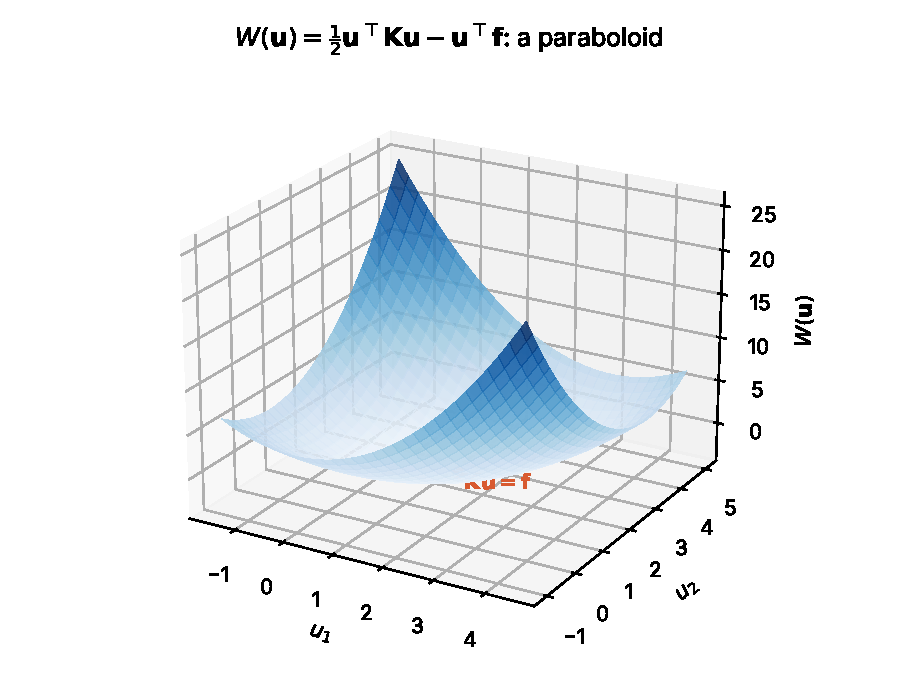
\includegraphics[width=0.6\textwidth]{figures/ch1/paraboloid.pdf}
\caption{The energy $W$ is a paraboloid: spring chain with unit stiffnesses,
$\vf=(1,1,1)\T$, sliced at the optimal $u_3$. The marked point solves
$\mat{K}\vu=\vf$, and $W_{\min}=-2.5=-\tfrac12\vf\T\mat{K}^{-1}\vf$.}
\label{fig:paraboloid}
\end{figure}

The positive definiteness of $\mat{K}$ can be quantified. Expanding $\vu$ in
\index{Rayleigh quotient}\index{coercivity!discrete}\index{boundedness!discrete}%
the orthonormal eigenbasis of $\mat{K}$ gives
\begin{equation}\label{eq:rayleigh}
  \lambda_{\min}\,|\vu|^2\le\vu\T\mat{K}\vu\le\lambda_{\max}\,|\vu|^2 .
\end{equation}
The lower bound is \emph{coercivity}, the upper bound \emph{boundedness}:
these are exactly the two hypotheses of the Lax--Milgram theorem of
Section~\ref{sec:var-lm}, here verified on a matrix
(Exercise~\ref{exo:lm-constants}).

\subsection{Symmetry, energy and path independence}\label{ssec:symmetry}
\index{symmetry!and existence of an energy}\index{path independence}%
Positive definiteness makes $W$ a genuine energy, bounded below and strictly
convex. Symmetry is what makes it exist at all. For a linear system
$\vF=\mat{K}\vu$, the work along a loading path from state $A$ to state $B$ is
\[
  \int_A^B\vF\cdot\dot\vu\dd t=\int_A^B\dot\vu\T\mat{K}\vu\dd t
  =\tfrac12\bigl[\vu\T\mat{K}\vu\bigr]_A^B
\]
\emph{if and only if $\mat{K}$ is symmetric}. Otherwise the work depends on
the path and not only on the end points, and no state function exists. The
same holds for bilinear forms: a symmetric form $a(u,v)$ has the energy
$J(u)=\tfrac12a(u,u)-L(u)$, a non-symmetric one generally has none
(Exercises~\ref{exo:guess-energy} and~\ref{exo:no-energy}).

\subsection{Reciprocity: the Maxwell--Betti theorem}\label{ssec:reciprocity}
\index{reciprocity!Maxwell--Betti}\index{Maxwell--Betti theorem}\index{Faraday experiment}%
\begin{figure}[h]
\centering
\begin{tikzpicture}[scale=1]
  \draw[thick] (0,0) -- (0,1);
  \foreach \y in {0,0.2,0.4,0.6,0.8,1} \draw (0,\y) -- (-0.18,\y-0.18);
  \draw[thick] (0,0.5) -- (4.2,0.5);
  \draw[arr,color=orange!80!black] (1.2,0.5) -- (1.2,1.1);
  \node[above,font=\small] at (1.2,1.15) {$F^{(1)}$};
  \node[below,font=\small] at (1.2,0.35) {$P$};
  \draw[arr,color=cu] (3.2,0.5) -- (3.2,0.9);
  \node[above,font=\small] at (3.2,0.95) {$u^{(1)}_Q$};
  \node[below,font=\small] at (3.2,0.35) {$Q$};
  \node[font=\sffamily\small] at (2.1,-0.35) {load case 1};
  \begin{scope}[xshift=6cm]
  \draw[thick] (0,0) -- (0,1);
  \foreach \y in {0,0.2,0.4,0.6,0.8,1} \draw (0,\y) -- (-0.18,\y-0.18);
  \draw[thick] (0,0.5) -- (4.2,0.5);
  \draw[arr,color=cu] (1.2,0.5) -- (1.2,0.9);
  \node[above,font=\small] at (1.2,0.95) {$u^{(2)}_P$};
  \node[below,font=\small] at (1.2,0.35) {$P$};
  \draw[arr,color=orange!80!black] (3.2,0.5) -- (3.2,1.1);
  \node[above,font=\small] at (3.2,1.15) {$F^{(2)}$};
  \node[below,font=\small] at (3.2,0.35) {$Q$};
  \node[font=\sffamily\small] at (2.1,-0.35) {load case 2};
  \end{scope}
\end{tikzpicture}
\caption{Reciprocity. Loading at $P$ and measuring at $Q$ gives the same
cross-work as loading at $Q$ and measuring at $P$:
$F^{(1)}u^{(2)}_P=F^{(2)}u^{(1)}_Q$.}
\label{fig:reciprocity}
\end{figure}
Loading a structure at $P$ and measuring the displacement at $Q$ gives the
same cross-work as loading at $Q$ and measuring at $P$
(Figure~\ref{fig:reciprocity}). This is the reciprocity principle, shown in
class as the ``Faraday experiment''.\footnote{In the literature the result is
credited to Clebsch ($\sim$1862), Maxwell (1864), Betti (1872) and Rayleigh
(1873).}\draftnote{Faraday attribution: keep as the name of the classroom demo?}

\begin{proposition}\label{prop:reciprocity}
\index{reciprocity!and symmetry}\index{flexibility matrix}%
Let $\vF=\mat{K}\vu$ with $\mat{K}$ invertible. The reciprocity identity
\[
  \vF^{(1)}\cdot\vu^{(2)}=\vF^{(2)}\cdot\vu^{(1)}
\]
holds for every pair of load cases if and only if $\mat{K}\T=\mat{K}$.
\end{proposition}
\begin{proof}
$\vF^{(1)}\cdot\vu^{(2)}=(\mat{K}\vu^{(1)})\T\vu^{(2)}=\vu^{(1)\top}\mat{K}\T\vu^{(2)}$
and $\vF^{(2)}\cdot\vu^{(1)}=\vu^{(1)\top}\mat{K}\vu^{(2)}$. They agree for all
$\vu^{(1)},\vu^{(2)}$ if and only if $\mat{K}\T=\mat{K}$. For unit loads at $P$
and $Q$, the displacements are columns of the flexibility matrix
$\mat{S}=\mat{K}^{-1}$, and reciprocity reads $S_{QP}=S_{PQ}$.
\end{proof}
In the continuum, reciprocity is Green's second identity
(Appendix~\ref{app:ibp}). When the body contains an unknown defect,
reciprocity between the true field and a known ``adjoint'' field is
\emph{broken}, and the gap measures the defect: this is the idea of
Chapter~\ref{ch:rg}.

\subsection{Circuits and trusses: the same linear algebra}
\paragraph{A resistor network.} Replace masses by nodes, displacements $\vu$ by
\index{resistor network}%
potentials and springs by resistors. Ohm's law $\sigma_i=c_ie_i$ is the
constitutive law, $\mat{C}=\diag(\text{conductances})$, and Kirchhoff's current
law at the nodes is exactly $\mat{B}\T\vect{\sigma}=\vf$ (injected currents).
With unit conductances the assembled matrix is the same $\mat{K}$: a resistor
ladder and a spring chain obey identical linear algebra. It is the discrete
analogue of $-\dive(\tA(\vx)\nabla u)=f$ (Section~\ref{sec:var-elliptic}).

\paragraph{A small truss.} Let $\mat{B}$ map joint displacements to bar
\index{truss}\index{energy!complementary (discrete)}%
elongations in a planar truss, $\mat{C}=\diag(E_iA_i/L_i)$ collect the bar
stiffnesses, and $\mat{B}\T\vect{\sigma}=\vf$ express the equilibrium of the
joints. Minimizing $W(\vu)$ is the discrete \emph{potential energy principle}.
Its dual, maximizing $-\tfrac12\vect{\sigma}\T\mat{C}^{-1}\vect{\sigma}$ over bar
tensions satisfying $\mat{B}\T\vect{\sigma}=\vf$, is the discrete
\emph{complementary energy principle}: the finite-dimensional counterpart of
the primal/dual pair of Section~\ref{sec:var-dual}, with $\mat{B}\T$ playing
the role of $-\dive$ and $\mat{C}^{-1}$ that of the conjugate energy.

%======================================================================
\section{Weak and strong forms: the right function space}\label{sec:var-weak}
\index{weak form}\index{strong form}\index{Sobolev space}\index{integration by parts!weak form}%
Integration by parts lowers the number of derivatives required, moving the
natural setting from $H^2$ down to $H^1$. This is why Sobolev spaces and
elliptic PDE theory are so intertwined~\cite{AdamsFournier2003,Evans2010}.
\begin{center}
\begin{tikzpicture}[node distance=1.6cm]
  \node[smallbox] (s) {Strong form \\ $-\Delta u = f,\ u \in H^2(\Omega)$};
  \node[smallbox, right=of s] (w) {Weak form \\
    $\int_\Omega \nabla u \cdot \nabla v = \int_\Omega f v,\ u,v \in H^1_0(\Omega)$};
  \draw[arr] (s) -- node[above, font=\small]{integrate} node[below,font=\small]{by parts} (w);
\end{tikzpicture}
\end{center}
Multiply $-\Delta u=f$ by a test function $v\in C_c^\infty(\Omega)$ and
integrate by parts (Green's first identity, Theorem~\ref{thm:green1}):
\[
  -\int_\Omega (\Delta u)\, v\dd x=\int_\Omega \nabla u \cdot \nabla v\dd x
  = \int_\Omega f v\dd x .
\]
The boundary term vanishes since $v=0$ near $\partial\Omega$. The left-hand
side only requires $u,v\in H^1$ (one derivative in $L^2$), so the identity
extends by density to all $v\in H^1_0(\Omega)$; there is no longer any need
for $u\in H^2$.

The weak form is also the first variation of the energy~\eqref{eq:poisson-energy}:
$\frac{\dd}{\dd t}J(u+tv)\big|_{t=0}=\int_\Omega\nabla u\cdot\nabla v-\int_\Omega fv$.
The three settings
\begin{center}
\begin{tabular}{lll}
\toprule
\sffamily energy & \sffamily weak form (virtual work) & \sffamily strong form (Euler--Lagrange)\\
\midrule
$\displaystyle u=\argmin_{v\in V}J(v)$ & $\delta J(u)[v]=0\ \ \forall v\in V$ & $-\Delta u=f$ in $\Omega$\\
\bottomrule
\end{tabular}
\end{center}
are equivalent for smooth solutions; their precise definitions are given in
Appendix~\ref{app:derivatives}.

%======================================================================
\section{Existence by minimization: the direct method}\label{sec:var-direct}
\index{direct method}\index{lower semicontinuity}\index{minimizing sequence}\index{Poincar\'e inequality}\index{coercivity!of an energy}%
Recasting a PDE as a minimization problem turns existence into the question
of whether a functional attains its infimum. Weak compactness and lower
semicontinuity answer it without constructing the solution~\cite{Dacorogna2008}.
\begin{center}
\begin{tikzpicture}[node distance=0.55cm]
  \node[box] (a) {Minimize $J(u)$ over $V$};
  \node[box, below=of a] (b) {Take a minimizing sequence $(u_n)$};
  \node[box, below=of b] (c) {Bounded $\Rightarrow$ weakly compact in $V$ (reflexive)};
  \node[box, below=of c] (d) {$J$ weakly lower semicontinuous};
  \node[box, goal, below=of d] (e) {Minimizer $u^\ast$ attained};
  \draw[arr] (a) -- (b); \draw[arr] (b) -- (c); \draw[arr] (c) -- (d); \draw[arr] (d) -- (e);
\end{tikzpicture}
\end{center}
For the energy~\eqref{eq:poisson-energy} on $V=H^1_0(\Omega)$:
\begin{itemize}
  \item \emph{coercivity:} by the Poincar\'e inequality
  $\norm{v}_{L^2}\le C_P\norm{\nabla v}_{L^2}$,
  \[
    J(v)\ge\tfrac12\norm{\nabla v}_{L^2}^2-C_P\norm{f}_{L^2}\norm{\nabla v}_{L^2}\to\infty
    \quad\text{as }\norm{v}_{H^1_0}\to\infty;
  \]
  in particular $J$ is bounded below;
  \item a minimizing sequence $(u_n)$ is therefore bounded in $H^1_0$, and a
  subsequence converges weakly to some $u$ (reflexivity);
  \item $J$ is convex and continuous, hence weakly lower semicontinuous:
  $J(u)\le\liminf J(u_n)=\inf J$.
\end{itemize}
So $u$ is a minimizer, and its first variation gives $-\Delta u=f$ in the weak
sense.

%======================================================================
\section{The Lax--Milgram theorem}\label{sec:var-lm}
\index{Lax--Milgram theorem}\index{coercivity!of a bilinear form}\index{boundedness!of a bilinear form}%
Two functional-analytic hypotheses on a bilinear form, boundedness and
coercivity, give existence \emph{and} uniqueness, independently of the
specific PDE~\cite{LaxMilgram1954}.

\begin{gbox}{Lax--Milgram theorem}
Let $V$ be a Hilbert space, $a:V\times V\to\R$ bilinear and $L\in V^\ast$.
If $a$ is \emph{bounded}, $|a(u,v)|\le M\norm{u}\norm{v}$, and \emph{coercive},
$a(u,u)\ge\alpha\norm{u}^2$ with $\alpha>0$, then there is a unique $u\in V$
such that
\[
  a(u,v)=L(v)\qquad\forall v\in V,
\]
and $\norm{u}\le\norm{L}_{V^\ast}/\alpha$. The form $a$ need not be symmetric.
\end{gbox}

For the model problem, $a(u,v)=\int_\Omega\nabla u\cdot\nabla v$ and
$L(v)=\int_\Omega fv$ on $H^1_0(\Omega)$:
\begin{itemize}
  \item \emph{bounded:} $|a(u,v)|\le\norm{\nabla u}_{L^2}\norm{\nabla v}_{L^2}$
  (Cauchy--Schwarz);
  \item \emph{coercive:} $a(u,u)=\norm{\nabla u}_{L^2}^2\ge\alpha\norm{u}_{H^1_0}^2$
  (Poincar\'e);
  \item $L$ is bounded: $|L(v)|\le\norm{f}_{L^2}\norm{v}_{L^2}\le C_P\norm{f}_{L^2}\norm{v}_{H^1_0}$.
\end{itemize}
Lax--Milgram gives existence and uniqueness directly, without mentioning
minimization. The discrete bounds~\eqref{eq:rayleigh} are the same two
hypotheses for a matrix.

\subsection*{What goes wrong without coercivity}
Boundedness alone is not enough. Two examples, one linear and one nonlinear,
show what breaks.

\paragraph{(a) A linear resonance.} On $H^1_0(0,1)$ take
\index{resonance}\index{Wirtinger inequality}\index{Fredholm alternative}%
\[
  a(u,v)=\int_0^1u'v'\dd x-\pi^2\int_0^1uv\dd x,
\]
corresponding to $-u''-\pi^2u=f$, $u(0)=u(1)=0$. The form is bounded,
$|a(u,v)|\le(1+\pi^2)\norm{u}_{H^1_0}\norm{v}_{H^1_0}$, but not coercive: the
sharp Poincar\'e (Wirtinger) inequality $\int_0^1(u')^2\ge\pi^2\int_0^1u^2$ is
an equality at $u=\sin\pi x$, so $a(\sin\pi x,\sin\pi x)=0$. This is not an
artefact of the proof: $\pi^2$ is the first Dirichlet eigenvalue of
$-\dd^2/\dd x^2$ on $(0,1)$, the problem is at resonance, and the Fredholm
alternative (Section~\ref{sec:var-elliptic}) takes over. Solvability requires
$f\perp\sin\pi x$ in $L^2$. For $f=1$, $\int_0^1\sin\pi x\dd x=2/\pi\neq0$:
\textbf{no solution}. For $f=\sin2\pi x$ the condition holds, and
$u_c=\sin(2\pi x)/(3\pi^2)+c\sin\pi x$ solves the problem for every
$c\in\R$: \textbf{infinitely many solutions} (Figure~\ref{fig:resonance}).

\begin{figure}[h]
\centering
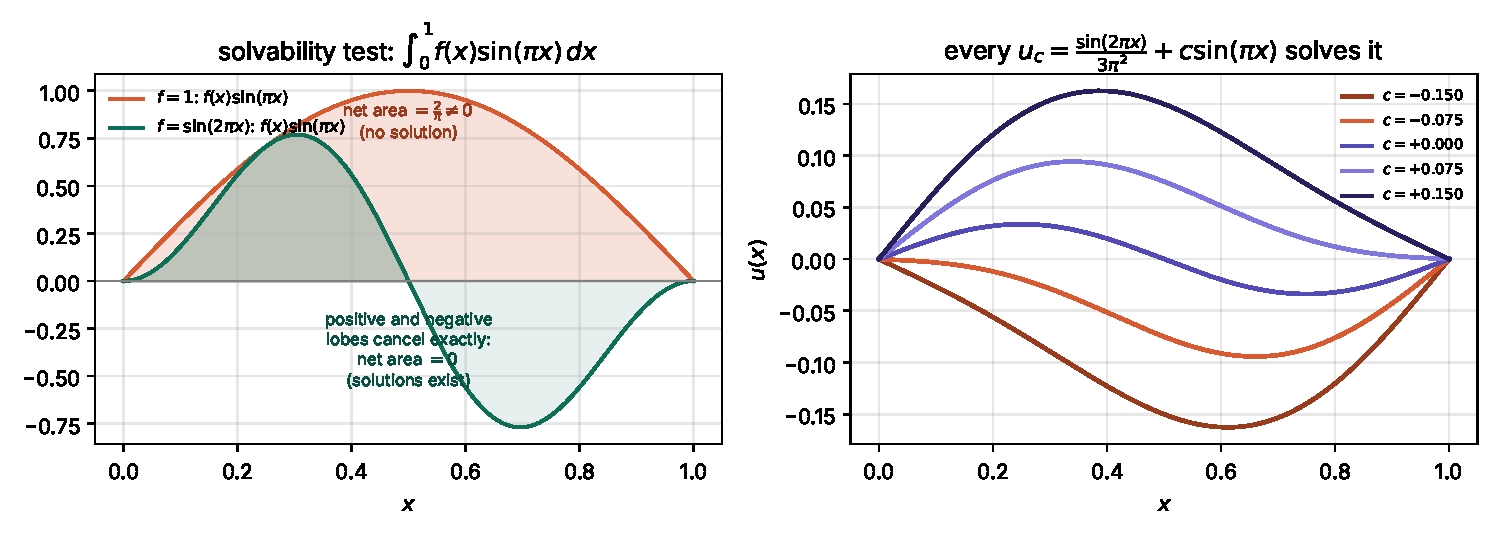
\includegraphics[width=\textwidth]{figures/ch1/resonance_example.pdf}
\caption{Resonance. Left: the solvability test $\int_0^1 f\sin\pi x\dd x$.
For $f=1$ the product stays positive and the integral is $2/\pi$: no
solution. For $f=\sin2\pi x$ the lobes cancel: solutions exist. Right: the
one-parameter family $u_c$ of solutions.}
\label{fig:resonance}
\end{figure}

\paragraph{(b) A nonlinear double well.} Lax--Milgram is a linear theorem, but
\index{double well}\index{Allen--Cahn equation}\index{second variation}\index{stability!of a critical point}%
the coercivity intuition reappears in the second variation. On $(0,1)$ take
\[
  E[u]=\int_0^1\Bigl(\frac{\varepsilon^2}{2}(u')^2+W(u)\Bigr)\dd x,
  \qquad W(u)=\tfrac14(u^2-1)^2,
\]
whose Euler--Lagrange equation is the stationary Allen--Cahn equation
$-\varepsilon^2u''+u^3-u=0$~\cite{AllenCahn1979}. Existence of a minimizer
still holds by the direct method (Rellich--Kondrachov compactness handles the
non-convex zeroth-order term), but uniqueness fails twice: by the symmetry
$u\mapsto-u$, $u\equiv1$ and $u\equiv-1$ are both global minimizers; and
$u\equiv0$ is a critical point whose second variation
\[
  \delta^2E(0)[v,v]=\varepsilon^2\int_0^1(v')^2\dd x-\int_0^1v^2\dd x
\]
is \emph{negative} for every nonzero constant $v$: $u\equiv0$ is unstable
(Figure~\ref{fig:doublewell}). Stability through the second variation is the
subject of the last part of the course.

\begin{figure}[h]
\centering
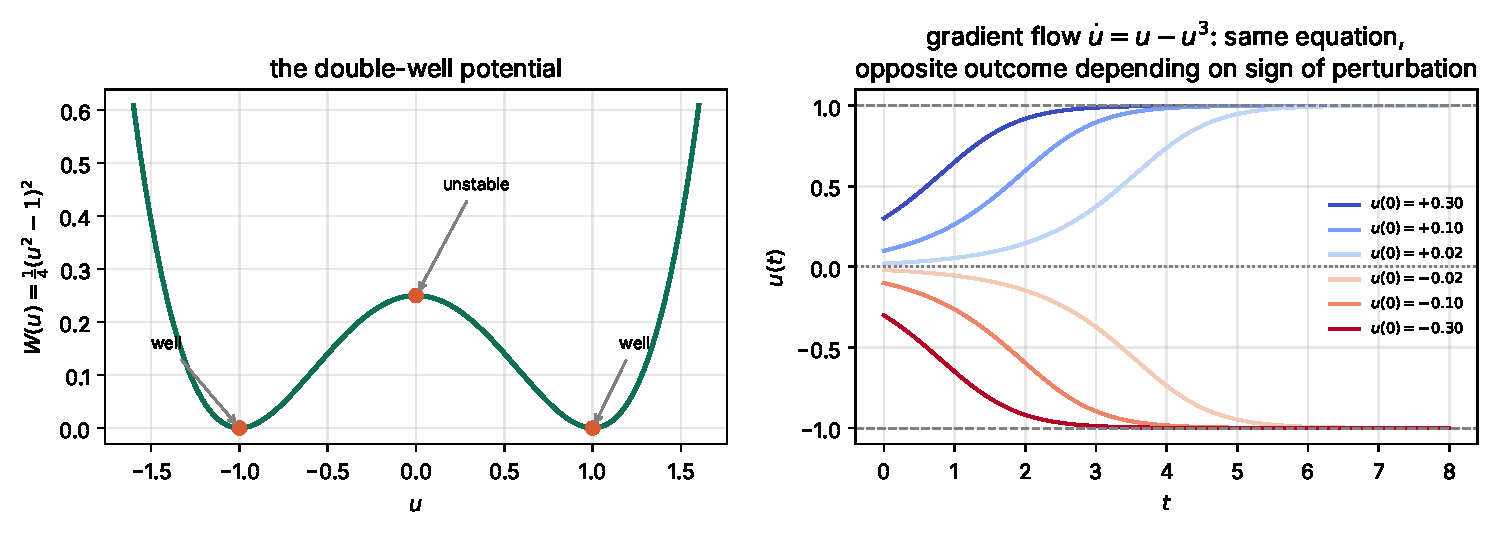
\includegraphics[width=\textwidth]{figures/ch1/doublewell_bistability.pdf}
\caption{Left: the double-well potential, minima at $u=\pm1$, unstable maximum
at $u=0$. Right: the gradient flow $\dot u=u-u^3$ from initial conditions near
$0$; a $\pm0.02$ perturbation decides whether the system ends at $+1$ or $-1$.}
\label{fig:doublewell}
\end{figure}

%======================================================================
\section{General elliptic operators}\label{sec:var-elliptic}
\index{elliptic operator!general}\index{uniform ellipticity}\index{G\aa rding inequality@G{\aa}rding inequality}%
The Poisson problem uses the simplest elliptic operator. The Lax--Milgram
framework is built for the general second-order case, where the minimization
approach does not always apply~\cite{GilbargTrudinger2001,Evans2010}.

\paragraph{The operator.} Consider
\begin{equation}\label{eq:general-elliptic}
  -\dive(\tA(\vx)\nabla u)+\vb(\vx)\cdot\nabla u+c(\vx)u=f
  \ \text{in } \Omega,\qquad u=0 \ \text{on } \partial\Omega,
\end{equation}
with $\tA(\vx)$ a second-order tensor field (conductivity, diffusivity),
$\vb$ a drift (convection) field and $c$ a reaction coefficient. The operator
is \emph{uniformly elliptic} if
$\vxi\cdot\tA(\vx)\vxi\ge\alpha|\vxi|^2$ for all $\vxi\in\R^n$, $\vx\in\Omega$,
some $\alpha>0$.

\paragraph{The bilinear form.} Integrating by parts with
Theorem~\ref{thm:ibp-matrix},
\[
  a(u,v)=\int_\Omega\tA\nabla u\cdot\nabla v\dd x
  +\int_\Omega(\vb\cdot\nabla u)\,v\dd x+\int_\Omega c\,uv\dd x .
\]

\paragraph{The hypotheses.} If $\tA,\vb,c\in L^\infty(\Omega)$, $a$ is bounded.
Ellipticity gives $\int\tA\nabla u\cdot\nabla u\ge\alpha\norm{\nabla u}^2_{L^2}$,
and Poincar\'e controls the full norm; but the lower-order terms can spoil
coercivity. G\aa rding's inequality~\cite{Garding1953},
\[
  a(u,u)\ge\alpha\norm{u}_{H^1_0}^2-\lambda\norm{u}_{L^2}^2,\qquad\lambda\ge0,
\]
states coercivity up to a compact perturbation. Either one shifts the form,
$a_\lambda(u,v)=a(u,v)+\lambda\int uv$, which is coercive, or one invokes the
\emph{Fredholm alternative}: the problem is solvable for all $f$ except on a
finite-dimensional exceptional set related to the eigenvalues of the operator.

\paragraph{Where Lax--Milgram goes further than minimization.} Lax--Milgram
\index{convection--diffusion}\index{symmetry!of a bilinear form}%
does not require $a$ to be symmetric; minimization does. A quadratic energy
$J(u)=\tfrac12a(u,u)-L(u)$ has $\delta J(u)[v]=a(u,v)-L(v)$ only when $a$ is
symmetric (Section~\ref{ssec:symmetry}). The convection term
$\int(\vb\cdot\nabla u)v$ is not symmetric, so convection--diffusion has no
natural energy, yet Lax--Milgram applies. Dirichlet, Neumann or Robin
conditions are handled by changing the space ($H^1_0$ or $H^1$) and adding
boundary terms to $a$ (Exercises~\ref{exo:neumann} and~\ref{exo:robin}).

%======================================================================
\section{Duality}\label{sec:var-dual}
\index{duality}\index{energy!complementary}%
Variational problems are optimization problems, so convex duality
applies~\cite{EkelandTemam1999,Rockafellar1970}: the primal (energy) problem
has a dual (complementary energy) problem, and for convex functionals the two
meet at the optimum.
\begin{center}
\begin{tikzpicture}[node distance=1.6cm]
  \node[smallbox] (p) {Primal problem \\ $\min_u J(u)$};
  \node[smallbox, right=of p] (d) {Dual problem \\ $\max_{\vp}\,-J^\ast(\vp)$};
  \draw[arr,{Latex[length=2.3mm]}-{Latex[length=2.3mm]}] (p) -- node[above, font=\small]{duality} (d);
\end{tikzpicture}
\end{center}

\subsection{The Legendre--Fenchel transform}
\begin{gbox}{Legendre--Fenchel transform}
\index{Legendre--Fenchel transform}\index{convex conjugate}\index{Fenchel--Young inequality}%
For a convex function $F$ on a space $X$, its conjugate on the dual space is
\[
  F^\ast(\vp)=\sup_{\vx}\bigl[\vp\cdot\vx-F(\vx)\bigr].
\]
\begin{itemize}
  \item $F^\ast$ is convex (a supremum of affine functions);
  \item Fenchel--Young inequality: $F(\vx)+F^\ast(\vp)\ge\vp\cdot\vx$ for all
  $\vx,\vp$, with equality iff $\vp\in\partial F(\vx)$;
  \item if $F$ is convex and lower semicontinuous, $F^{\ast\ast}=F$:
  $F(\vx)=\sup_{\vp}\bigl[\vp\cdot\vx-F^\ast(\vp)\bigr]$.
\end{itemize}
\end{gbox}
Geometrically, the tangent to $F$ with slope $p$ has vertical intercept
$-F^\ast(p)$ (Figure~\ref{fig:legendre}). Examples are worked out in
Exercise~\ref{exo:lf}.

\begin{figure}[h]
\centering
\begin{tikzpicture}[scale=0.85]
  \draw[->] (-0.5,0) -- (4,0) node[right] {$x$};
  \draw[->] (0,-2.7) -- (0,5.3) node[above] {$F(x)$};
  \draw[thick, cu, domain=0:3.2, smooth, variable=\x, samples=60]
    plot ({\x},{\x*\x/2}) node[right] {$F(x)=x^2/2$};
  \draw[thick, orange!80!black] (-0.25,-2.5) -- (3,4) node[right] {slope $p$};
  \filldraw[orange!80!black] (2,2) circle (1.5pt);
  \draw[dashed, gray] (2,2) -- (2,0) node[below] {$x_0$};
  \filldraw[orange!80!black] (0,-2) circle (1.5pt);
  \node[left] at (-0.1,-2) {$-F^\ast(p)$};
\end{tikzpicture}
\caption{The Legendre--Fenchel transform: $-F^\ast(p)$ is the intercept of
the tangent of slope $p$.}
\label{fig:legendre}
\end{figure}

\subsection{Constructing the dual of the Poisson problem}
\index{duality!Fenchel--Rockafellar}\index{adjoint operator!of the gradient}%
Split $J$ into two convex pieces joined by the linear operator
$\Lambda=\nabla$:
\[
  J(u)=F(\Lambda u)+G(u),\qquad
  F(\vp)=\tfrac12\int_\Omega|\vp|^2\dd x,\qquad
  G(u)=-\int_\Omega fu\dd x .
\]
\begin{enumerate}[label=\emph{Step \arabic*.},leftmargin=*,itemsep=3pt]
\item \emph{Conjugate of $F$.} A quadratic form on a Hilbert space is
self-conjugate: $F^\ast(\vp)=\tfrac12\int_\Omega|\vp|^2\dd x$.
\item \emph{Conjugate of $G$.} $G$ is linear, so its conjugate is an
indicator function:
$G^\ast(w)=\sup_u\int_\Omega(w+f)u\dd x$ equals $0$ if $w=-f$ and $+\infty$
otherwise.
\item \emph{The adjoint $\Lambda^\ast$.} Integrating by parts (the boundary
term vanishes in $H^1_0$), $\int_\Omega\vp\cdot\nabla u=-\int_\Omega(\dive\vp)\,u$,
so $\Lambda^\ast\vp=-\dive\vp$.
\item \emph{Assemble.} Fenchel--Rockafellar duality states
\[
  \inf_u\bigl[F(\Lambda u)+G(u)\bigr]
  =\sup_{\vp}\bigl[-F^\ast(\vp)-G^\ast(-\Lambda^\ast\vp)\bigr].
\]
The term $G^\ast(-\Lambda^\ast\vp)$ is $0$ exactly when $\dive\vp+f=0$ and
$+\infty$ otherwise: it becomes a constraint.
\end{enumerate}

\begin{gbox}{Primal and dual problems}
\index{primal problem}\index{dual problem}%
\[
  \min_{u\in H^1_0(\Omega)}\Bigl(\tfrac12\int_\Omega|\nabla u|^2-\int_\Omega fu\Bigr)
  \;=\;
  \max_{\vp:\ \dive\vp+f=0}\Bigl(-\tfrac12\int_\Omega|\vp|^2\Bigr).
\]
At the optimum $\vp=\nabla u$, and both values equal $-\tfrac12\int_\Omega|\nabla u|^2$.
\end{gbox}
There is no duality gap because $F$ is continuous and finite everywhere and
$\Lambda$ is bounded, the standard qualification condition. This is the
statement that the minimum of the potential energy (over kinematically
admissible fields) and the maximum of the complementary energy (over
statically admissible fields) meet at the solution. It is used in elasticity
(Chapter~\ref{ch:elliptic}) and in a posteriori error estimation. Its
discrete counterpart is the truss of Section~\ref{sec:var-discrete}, and
Exercise~\ref{exo:primal-dual} checks it numerically.

%======================================================================
\section{Constraints and Lagrange multipliers}\label{sec:var-lagrange}
\index{constraint}\index{Lagrange multiplier}\index{Lagrangian}%
Many problems minimize an energy under constraints: imposed displacements,
incompressibility, contact, plasticity. The Lagrangian turns the constrained
problem into an unconstrained saddle-point problem.

\begin{gbox}{Constrained optimization}
\index{Karush--Kuhn--Tucker conditions}\index{saddle point}\index{complementarity condition}%
Let $C$ and $\vect{A}=(A_1,\dots,A_m)$ be convex functions on $\R^n$.
\begin{itemize}
\item \emph{Problem $\mathcal P$:} minimize $C(\vx)$ under the constraint
$\vect{A}(\vx)\le\vb$.
\item \emph{Lagrangian:}
$\mathcal L(\vx,\vect{y})=C(\vx)+\vect{y}\cdot\bigl(\vect{A}(\vx)-\vb\bigr)$,
$\vect{y}\in\R^m$.
\item \emph{Karush--Kuhn--Tucker conditions.} If $\vx$ solves $\mathcal P$
(and a qualification condition holds), there is $\vect{y}\ge\vzero$ with
\[
  \nabla C(\vx)+\sum_iy_i\nabla A_i(\vx)=\vzero,\qquad
  \vect{y}\ge\vzero,\quad\vect{A}(\vx)\le\vb,\quad
  y_i\bigl(A_i(\vx)-b_i\bigr)=0\ \ \forall i .
\]
\end{itemize}
For equality constraints $\vect{A}(\vx)=\vb$ the multipliers have no sign,
and the conditions reduce to $\nabla_{\vx}\mathcal L=\vzero$,
$\nabla_{\vect{y}}\mathcal L=\vzero$: $(\vx,\vect{y})$ is a saddle point of
$\mathcal L$.
\end{gbox}

\begin{figure}[h]
\centering
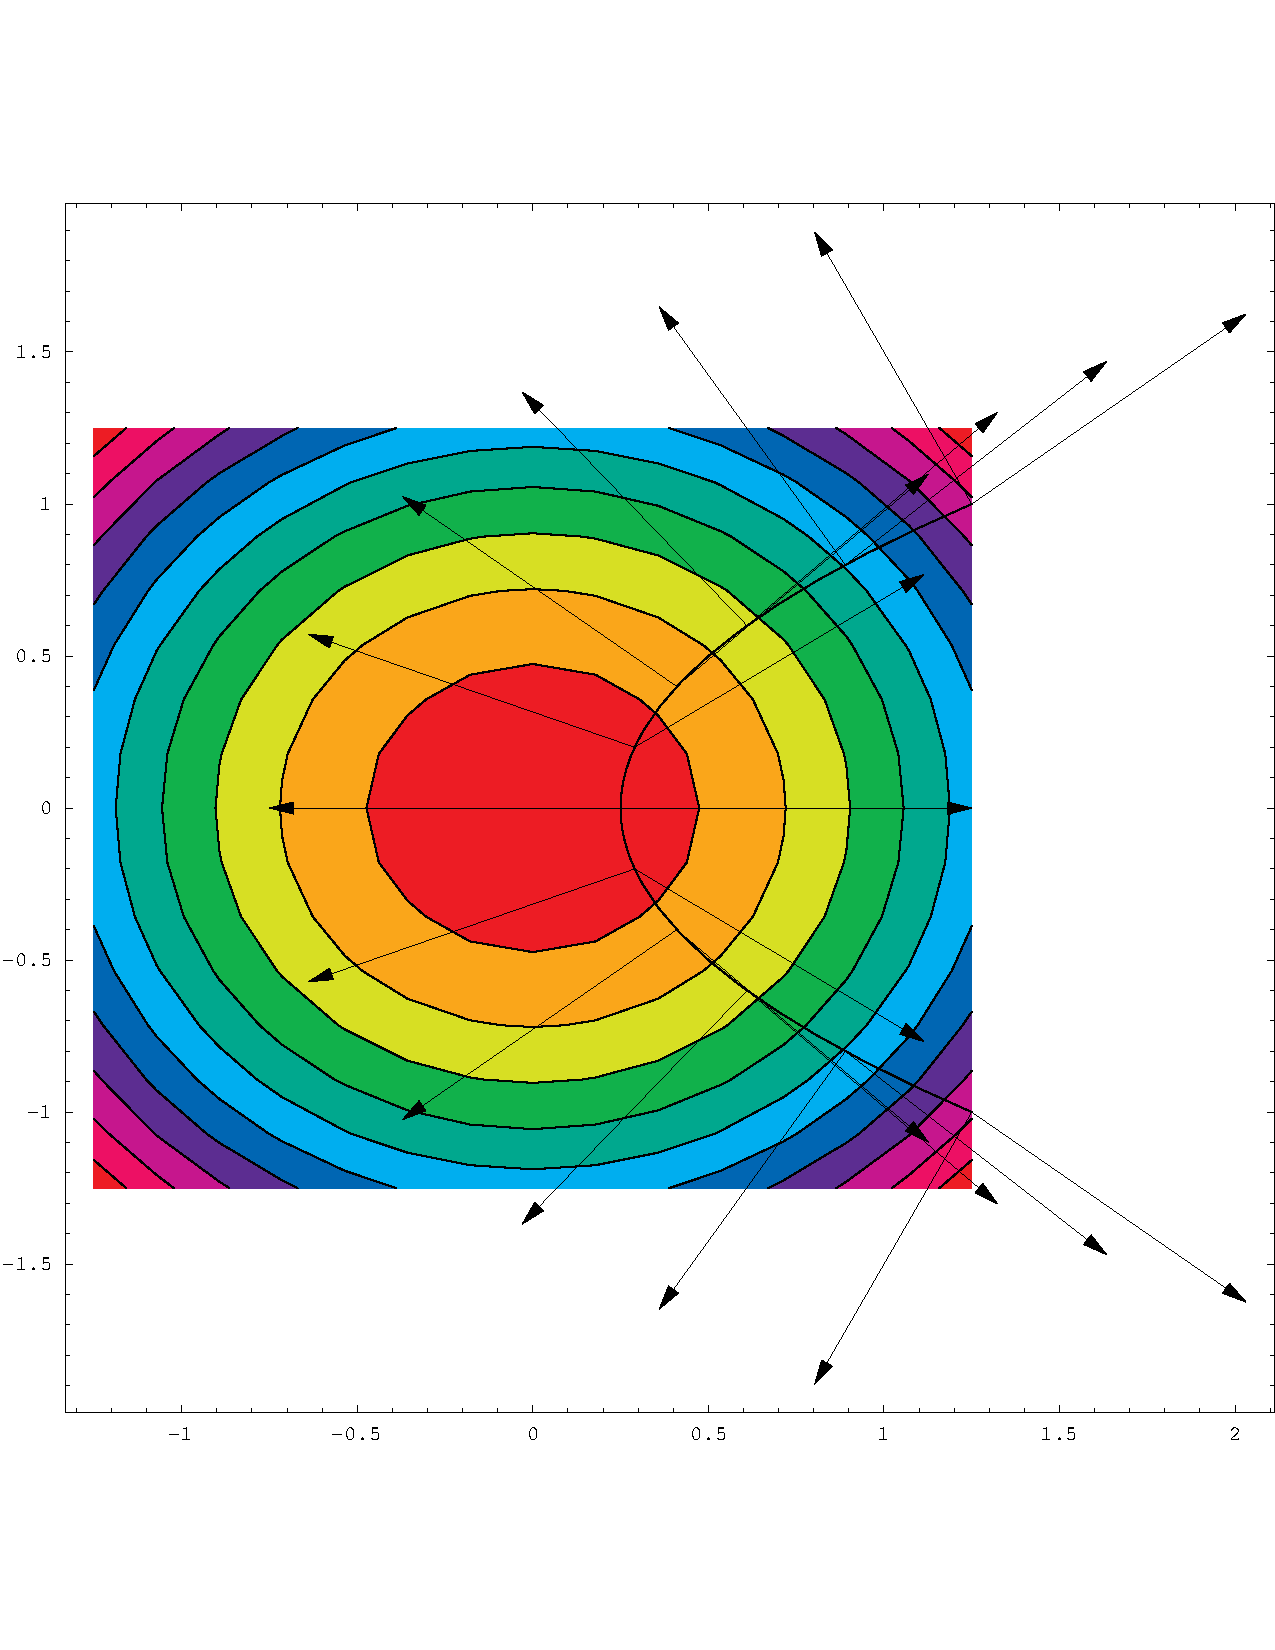
\includegraphics[height=5cm]{figures/ch1/lagrange.pdf}
\caption{Level sets of a convex cost $C$ and a constraint. At the constrained
minimum the gradient of $C$ is balanced by a multiple of the gradient of the
constraint.}
\label{fig:lagrange}
\end{figure}

The last condition is \emph{complementarity}: either the constraint is
active, $A_i(\vx)=b_i$, or its multiplier vanishes. The multiplier is the
force needed to enforce the constraint. In Chapter~\ref{ch:elliptic},
imposed displacements in a Ritz approximation are enforced this way, and the
multipliers are the reaction forces (Section~\ref{ssec:ritz-lagrange}).
Exercises~\ref{exo:kkt1}--\ref{exo:kkt4} work through four cases.

%======================================================================
\section{Galerkin approximation and finite elements}\label{sec:var-fem}
\index{Galerkin method}\index{C\'ea's lemma@C\'ea's lemma}\index{finite element method!one-dimensional}\index{stiffness matrix}%
The weak formulation is exactly what finite element methods discretize:
restrict the problem to a finite-dimensional subspace, solve a linear system,
and control the error with C\'ea's lemma~\cite{Cea1964}
(see also~\cite{Ciarlet2002,BrennerScott2008}).
\begin{center}
\begin{tikzpicture}[node distance=0.55cm]
  \node[box] (a) {Continuous problem in $V$: \ $a(u,v) = L(v)$, infinite-dimensional};
  \node[box, below=of a] (b) {Discrete problem in $V_h \subset V$: \ $a(u_h,v_h) = L(v_h)$};
  \node[box, key, below=of b] (c) {C\'ea's lemma: \ $\norm{u-u_h} \le \frac{M}{\alpha} \inf_{v_h\in V_h} \norm{u-v_h}$};
  \draw[arr] (a) -- (b); \draw[arr] (b) -- (c);
\end{tikzpicture}
\end{center}
Take the one-dimensional problem $-u''=f$ on $(0,1)$, $u(0)=u(1)=0$, with weak
form $\int_0^1u'v'=\int_0^1fv$.
\begin{itemize}
  \item Partition $[0,1]$ into $n$ intervals of size $h=1/n$ and let
  $V_h\subset H^1_0$ be spanned by the piecewise-linear ``hat'' functions
  $\varphi_1,\dots,\varphi_{n-1}$.
  \item Write $u_h=\sum_jc_j\varphi_j$ and require
  $\int u_h'\varphi_i'=\int f\varphi_i$ for each $i$: this is the linear
  system $\mat{K}\mat{c}=\mat{F}$ with the tridiagonal stiffness matrix
  $K_{ij}=\int\varphi_i'\varphi_j'=h^{-1}\operatorname{tridiag}(-1,2,-1)$,
  the matrix of the spring chain.
  \item C\'ea's lemma gives $\norm{u-u_h}_{H^1_0}\le C\inf_{v_h}\norm{u-v_h}_{H^1_0}=O(h)$
  for smooth $u$; nodal values converge faster (Exercise~\ref{exo:conv}).
\end{itemize}
Finite elements for elasticity, with the matrices $\mat{B}$, $\mat{C}$ and
$\mat{B}\T\mat{C}\mat{B}$ of Section~\ref{sec:var-discrete}, are presented in
Chapter~\ref{ch:elliptic}.

%======================================================================
\section{Physical interpretation: energies come first}\label{sec:var-phys}
\index{minimal surface}\index{soap film}%
Many equations of physics and geometry \emph{are} Euler--Lagrange equations of
an energy or action~\cite{GilbargTrudinger2001}: the PDE is a consequence of a
minimization principle, not an artificial reformulation.
\begin{center}
\begin{tikzpicture}[node distance=0.55cm]
  \node[box] (a) {Energy functional $E[u]$ \ (surface area, elastic energy, \dots)};
  \node[box, below=of a] (b) {Critical point: $\delta E(u) = 0$};
  \node[box, goal, below=of b] (c) {Euler--Lagrange equation (PDE), e.g.\ minimal surface equation};
  \draw[arr] (a) -- (b); \draw[arr] (b) -- (c);
\end{tikzpicture}
\end{center}
The area of the graph of $u$ over $\Omega$ is
\[
  A[u]=\int_\Omega\sqrt{1+|\nabla u|^2}\dd x .
\]
A soap film spanning a wire frame (the boundary data) minimizes it. The first
variation $\frac{\dd}{\dd t}A[u+t\varphi]\big|_{t=0}=0$ for all test functions
$\varphi$ gives, after integration by parts (Theorem~\ref{thm:ibp}),
\[
  \dive\!\left(\frac{\nabla u}{\sqrt{1+|\nabla u|^2}}\right)=0,
\]
the minimal surface equation~\cite{Courant1950}. The energy comes first
physically; the PDE follows. The same holds for elasticity, where the stored
energy $\tfrac12\eps:\bbC:\eps$ comes first and the Navier equations follow
(Chapter~\ref{ch:elliptic}).

%======================================================================
\framepart{Summary}
\begin{gbox*}
\begin{itemize}
  \item \textbf{Existence} follows from minimizing a coercive, weakly lower
  semicontinuous energy over a reflexive space
  (Section~\ref{sec:var-direct}); more generally, and without symmetry, from
  the Lax--Milgram theorem (Section~\ref{sec:var-lm}), which covers general
  elliptic operators through G\aa rding's inequality and the Fredholm
  alternative (Section~\ref{sec:var-elliptic}).
  \item \textbf{The weak form} is not an approximation of the strong form
  but a genuine widening of the solution space, made possible by integration
  by parts (Appendix~\ref{app:ibp}).
  \item \textbf{Duality} (Section~\ref{sec:var-dual}) gives every convex
  variational problem a mirror dual problem through the Legendre--Fenchel
  transform; the two meet at the optimum. \textbf{Constraints} enter through
  Lagrange multipliers (Section~\ref{sec:var-lagrange}).
  \item \textbf{The same linear algebra}, $\mat{B}\T\mat{C}\mat{B}\,\vu=\vf$,
  underlies springs, circuits, trusses (Section~\ref{sec:var-discrete}) and
  finite elements (Section~\ref{sec:var-fem}): compatibility, constitutive
  law and equilibrium, with equilibrium the transpose of compatibility.
  \item \textbf{Not every weak form has an energy.} A symmetric form has
  $J(u)=\tfrac12a(u,u)-L(u)$; a non-symmetric one (convection) has none,
  yet Lax--Milgram still applies.
\end{itemize}
\end{gbox*}
The same pattern (energy, weak form, abstract existence theorem, duality,
discretization) appears in linear elasticity, Stokes flow, image denoising by
total variation, and many machine learning objectives written as regularized
energy minimization.

%======================================================================
\framepart{Exercises}\label{sec:var-exo}
Part~I checks results numerically or symbolically: every script was run
(\texttt{numpy}/\texttt{scipy} for numerical checks, \texttt{sympy} for
symbolic ones) and its output is quoted in the comments. Part~II is
paper-and-pencil practice with variational calculus. Part~III treats
constraints and convex conjugates. Solutions are given in small type after
each exercise.

\framesub{Part I: computational verification}

\exercise{Minimizing by gradient descent}\label{exo:gd}
\index{gradient descent}%
For the spring chain ($\mat{K}=\operatorname{tridiag}(-1,2,-1)$,
$\vf=(1,1,1)\T$), minimize $W(\vu)=\tfrac12\vu\T\mat{K}\vu-\vf\T\vu$ by
gradient descent and compare with the direct solution of $\mat{K}\vu=\vf$.
What is the convergence rate?
\begin{solution}
\begin{lstlisting}
import numpy as np
K = np.array([[2,-1,0],[-1,2,-1],[0,-1,2]], dtype=float)
f = np.array([1,1,1], dtype=float)
u, step = np.zeros(3), 0.2
for _ in range(500):
    u -= step * (K @ u - f)              # gradient of W is K u - f
print(np.round(u, 4), np.round(np.linalg.solve(K, f), 4))
# [1.5 2.  1.5] [1.5 2.  1.5]   max difference ~ 1e-15
\end{lstlisting}
The error is multiplied at each step by $\mat{I}-\text{step}\,\mat{K}$, so it
contracts at the rate $\rho=\max_i|1-\text{step}\,\lambda_i(\mat{K})|$
(Figure~\ref{fig:gd}); the eigenvalues are those of Exercise~\ref{exo:lm-constants}.
\end{solution}

\begin{figure}[h]
\centering
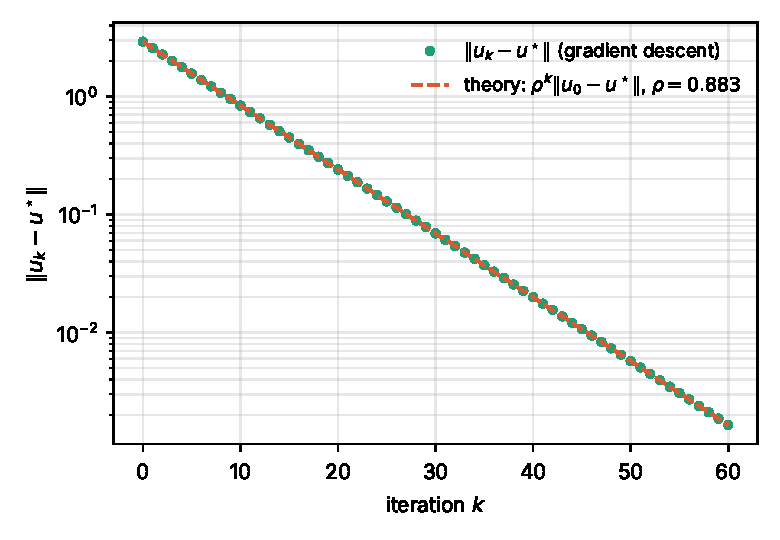
\includegraphics[width=0.55\textwidth]{figures/ch1/ex1_gd_convergence.pdf}
\caption{Exercise~\ref{exo:gd}: the observed convergence of gradient descent
follows the predicted rate $\rho=\max_i|1-\text{step}\,\lambda_i(\mat{K})|$.}
\label{fig:gd}
\end{figure}

\exercise{Integration by parts, checked numerically}\label{exo:ibp-num}
Verify $\int_0^1u'v'\dd x=-\int_0^1u''v\dd x+[u'v]_0^1$ for $u=\sin\pi x$,
$v=x(1-x)$.
\begin{solution}
\begin{lstlisting}
from scipy.integrate import quad
import numpy as np
du  = lambda x: np.pi*np.cos(np.pi*x)
d2u = lambda x: -np.pi**2*np.sin(np.pi*x)
v   = lambda x: x*(1-x);  dv = lambda x: 1-2*x
lhs = quad(lambda x: du(x)*dv(x), 0, 1)[0]
rhs = quad(lambda x: -d2u(x)*v(x), 0, 1)[0] + du(1)*v(1) - du(0)*v(0)
print(lhs, rhs)        # 1.27323954 1.27323954  (= 4/pi)
\end{lstlisting}
\end{solution}

\exercise{Lax--Milgram constants from eigenvalues}\label{exo:lm-constants}
(a) Compute the eigenvalues of the matrix $\mat{K}$ of the spring chain.
(b) Plot the points $(|\vu|^2,\vu\T\mat{K}\vu)$ for many random $\vu$.
(c) Propose two lines bounding the plot. (d) Relate them to the Lax--Milgram
theorem.
\begin{solution}
(a) $\lambda=2-\sqrt2,\ 2,\ 2+\sqrt2$, i.e.\ $0.5858,\ 2,\ 3.4142$.
(b)--(c) Because $\mat{K}$ is symmetric it has an orthonormal eigenbasis
$\ve_1,\ve_2,\ve_3$. Writing $\vu=\sum c_i\ve_i$,
$\vu\T\mat{K}\vu=\sum\lambda_ic_i^2$ and $|\vu|^2=\sum c_i^2$, so
$\alpha|\vu|^2\le\vu\T\mat{K}\vu\le M|\vu|^2$ with $\alpha=\lambda_{\min}$,
$M=\lambda_{\max}$. Both bounds are sharp: equality at $\vu=\ve_1$ and
$\vu=\ve_3$ (Figure~\ref{fig:coercivity}).
(d) The lower line is coercivity, the upper line boundedness: the two
hypotheses of Lax--Milgram, here for the bilinear form $a(\vu,\vv)=\vu\T\mat{K}\vv$.
\begin{lstlisting}
import numpy as np
K = np.array([[2,-1,0],[-1,2,-1],[0,-1,2]], dtype=float)
lam = np.linalg.eigvalsh(K); alpha, M = lam[0], lam[-1]
rng = np.random.default_rng(0)
for _ in range(5):
    u = rng.normal(size=3); a = u @ K @ u
    print(alpha*u@u <= a <= M*u@u)          # True, five times
\end{lstlisting}
\end{solution}

\begin{figure}[h]
\centering
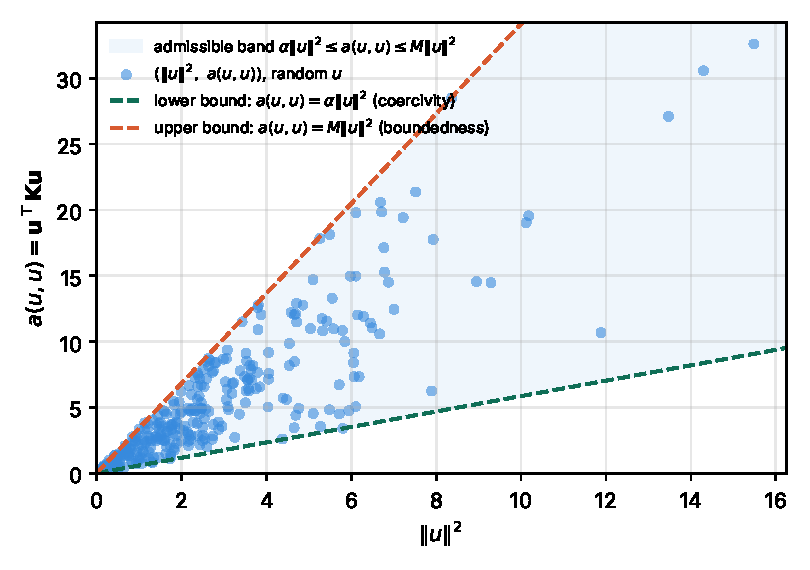
\includegraphics[width=0.6\textwidth]{figures/ch1/ex3_coercivity.pdf}
\caption{Exercise~\ref{exo:lm-constants}: $300$ random vectors $\vu$, plotted
as $(|\vu|^2,\vu\T\mat{K}\vu)$, lie in the band between coercivity
($\alpha|\vu|^2$) and boundedness ($M|\vu|^2$).}
\label{fig:coercivity}
\end{figure}

\exercise{Primal--dual equality for the spring chain}\label{exo:primal-dual}
With $\ve=\mat{B}\vu$ and unit stiffnesses, check that the potential energy
$W(\vu^\ast)$ equals the complementary energy $-\tfrac12|\vect{\sigma}^\ast|^2$
at $\vect{\sigma}^\ast=\mat{B}\vu^\ast$.
\begin{solution}
\begin{lstlisting}
import numpy as np
B = np.array([[1,0,0],[-1,1,0],[0,-1,1],[0,0,-1]], dtype=float)
K, f = B.T @ B, np.ones(3)
u = np.linalg.solve(K, f); s = B @ u
print(0.5*u@K@u - f@u, -0.5*s@s)   # -2.5 -2.5
\end{lstlisting}
Analytically: $W(\vu^\ast)=\tfrac12\vu^{\ast\top}\mat{K}\vu^\ast-\vf\T\vu^\ast=-\tfrac12\vu^{\ast\top}\mat{K}\vu^\ast=-\tfrac12|\mat{B}\vu^\ast|^2$,
the value $W_{\min}$ of Theorem~\ref{thm:min-discrete}.
\end{solution}

\exercise{Convergence rate of the discrete chain}\label{exo:conv}
\index{convergence rate}%
Solve $-u''=\sin\pi x$ on $(0,1)$, $u(0)=u(1)=0$ (exact solution
$\sin(\pi x)/\pi^2$) with the chain matrix for increasing $n$ and measure the
convergence rate.
\begin{solution}
\begin{lstlisting}
import numpy as np
def err(n):
    h = 1.0/(n+1); x = np.linspace(h, 1-h, n)
    K = (2*np.eye(n) - np.eye(n,k=1) - np.eye(n,k=-1))/h**2
    u = np.linalg.solve(K, np.sin(np.pi*x))
    return h, np.max(np.abs(u - np.sin(np.pi*x)/np.pi**2))
for n in [3, 7, 15, 31, 63]: print(*err(n))
# the error is divided by 4 when h is halved: O(h^2)
\end{lstlisting}
The nodal error is $O(h^2)$ (Figure~\ref{fig:conv}), better than the general
$O(h)$ energy-norm bound of C\'ea's lemma, thanks to the smoothness of the
solution.
\end{solution}

\begin{figure}[h]
\centering
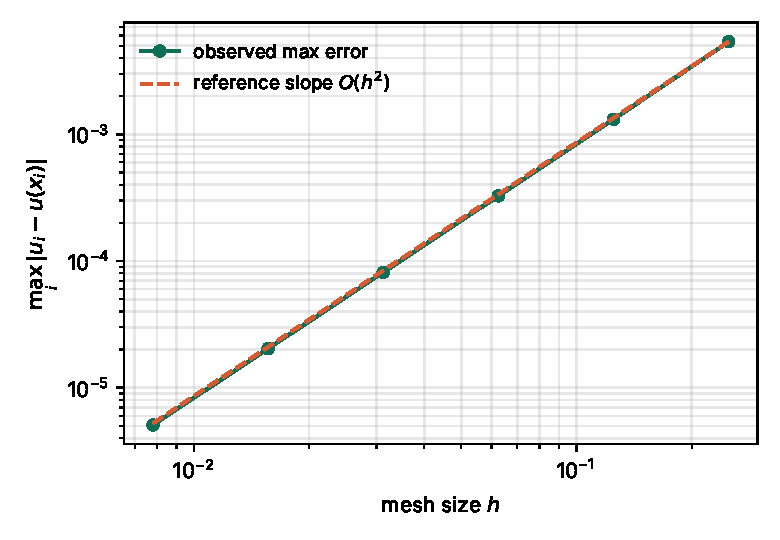
\includegraphics[width=0.55\textwidth]{figures/ch1/ex5_convergence_loglog.pdf}
\caption{Exercise~\ref{exo:conv}: maximal nodal error against $h$; slope $2$.}
\label{fig:conv}
\end{figure}

\exercise{Green's first identity on the unit cube}\label{exo:green-cube}
Verify Green's first identity (Theorem~\ref{thm:green1}) on $\Omega=(0,1)^3$
for $u=xy$, $v=yz$, computing both sides exactly.
\begin{solution}
$\nabla u\cdot\nabla v=(y,x,0)\cdot(0,z,y)=xz$, so the left-hand side is
$\int xz=\tfrac14$. Since $\Delta v=0$, the right-hand side is the boundary
term $\int_{\partial\Omega}u\,\partial_nv$: the faces $z=0$ and $z=1$ give
$\mp\tfrac16$ and cancel, the face $y=1$ gives $\int_0^1\!\!\int_0^1xz\dd x\dd z=\tfrac14$, the others $0$.
\begin{lstlisting}
import sympy as sp
x, y, z = sp.symbols('x y z'); u, v = x*y, y*z
lhs = sp.integrate(sum(sp.diff(u,s)*sp.diff(v,s) for s in (x,y,z)),
                   (x,0,1),(y,0,1),(z,0,1))
faces = [(x,0,-1,(y,z)),(x,1,1,(y,z)),(y,0,-1,(x,z)),
         (y,1,1,(x,z)),(z,0,-1,(x,y)),(z,1,1,(x,y))]
bnd = sum(sp.integrate((u*sg*sp.diff(v,w)).subs(w,val),(a,0,1),(b,0,1))
          for w,val,sg,(a,b) in faces)
print(lhs, bnd)        # 1/4 1/4
\end{lstlisting}
\end{solution}

\exercise{A non-symmetric bilinear form is still solvable}\label{exo:skew}
Add a skew-symmetric convection matrix $b\,\mat{S}$ to the diffusion matrix
$\mat{K}$. Check that $\vu\T(\mat{K}+b\mat{S})\vu=\vu\T\mat{K}\vu$, that
$\mat{K}+b\mat{S}$ is non-symmetric for $b\neq0$, and that the system remains
uniquely solvable.
\begin{solution}
\begin{lstlisting}
import numpy as np
n, h = 5, 1/6
K = (2*np.eye(n) - np.eye(n,k=1) - np.eye(n,k=-1))/h**2
S = (np.eye(n,k=1) - np.eye(n,k=-1))/(2*h)       # S^T = -S
rng = np.random.default_rng(1)
for b in [0.0, 5.0, 50.0]:
    A = K + b*S; u = rng.normal(size=n)
    print(b, np.allclose(A, A.T), np.isclose(u@A@u, u@K@u),
          np.linalg.norm(np.linalg.solve(A, np.ones(n))))
# symmetric only for b = 0; quadratic form unchanged; always solvable
\end{lstlisting}
The skew part vanishes on the diagonal $\vu\T\mat{S}\vu=0$, so coercivity is
unaffected: this is why Lax--Milgram applies without symmetry
(Section~\ref{sec:var-elliptic}).
\end{solution}

\exercise{Reciprocity, componentwise}\label{exo:reciprocity}
Split the degrees of freedom of $\vF=\mat{K}\vu$ into two groups $P$ and $Q$,
\[
  \begin{bmatrix}\vF_P\\ \vF_Q\end{bmatrix}=
  \begin{bmatrix}\mat{K}_{PP}&\mat{K}_{PQ}\\ \mat{K}_{QP}&\mat{K}_{QQ}\end{bmatrix}
  \begin{bmatrix}\vu_P\\ \vu_Q\end{bmatrix}.
\]
Load case 1 loads only $P$, load case 2 only $Q$. Write the reciprocity
identity in blocks and show that it holds for all loads iff
$\mat{K}_{QP}=\mat{K}_{PQ}\T$ (with $\mat{K}_{PP}$, $\mat{K}_{QQ}$ symmetric).
Check it numerically on the spring chain with $P=\{1\}$, $Q=\{3\}$.
\begin{solution}
With $\mat{S}=\mat{K}^{-1}$, case 1 gives $\vu^{(1)}=\mat{S}_{\cdot P}\vF_P^{(1)}$
and case 2 gives $\vu^{(2)}=\mat{S}_{\cdot Q}\vF_Q^{(2)}$. Reciprocity
$\vF^{(1)}\cdot\vu^{(2)}=\vF^{(2)}\cdot\vu^{(1)}$ reads
$\vF_P^{(1)}\cdot\mat{S}_{PQ}\vF_Q^{(2)}=\vF_Q^{(2)}\cdot\mat{S}_{QP}\vF_P^{(1)}$
for all loads, i.e.\ $\mat{S}_{QP}=\mat{S}_{PQ}\T$. Taking also $P=Q$ groups
gives the symmetry of the diagonal blocks, so $\mat{S}$, hence $\mat{K}$, is
symmetric. For the chain, $\mat{S}=\tfrac14\begin{psmallmatrix}3&2&1\\2&4&2\\1&2&3\end{psmallmatrix}$:
a unit load at node~1 moves node~3 by $\tfrac14$, and a unit load at node~3
moves node~1 by $\tfrac14$.
\end{solution}

\framesub{Part II: variational calculus practice}

\paragraph{From energy to strong form, through the weak form.}

\exercise{Natural boundary conditions}\label{exo:neumann}
\index{boundary condition!natural}\index{boundary condition!essential}\index{boundary condition!Neumann}\index{compatibility condition}%
On $\Omega=(0,1)$ consider, over the unconstrained space $V=H^1(0,1)$,
\[
  E[u]=\int_0^1\tfrac12(u')^2\dd x-\int_0^1fu\dd x-g\,u(1).
\]
Derive the weak form, then the strong form and the boundary conditions. What
happens at $x=0$, where $E$ has no boundary term? Is the problem well posed?
\begin{solution}
The first variation is
$\delta E(u)[\varphi]=\int_0^1u'\varphi'-\int_0^1f\varphi-g\varphi(1)=0$ for
all $\varphi\in H^1(0,1)$: this is the weak form. Integrating by parts,
$\int_0^1u'\varphi'=-\int_0^1u''\varphi+u'(1)\varphi(1)-u'(0)\varphi(0)$, so
\[
  \int_0^1(-u''-f)\varphi\dd x+\bigl(u'(1)-g\bigr)\varphi(1)-u'(0)\varphi(0)=0
  \quad\forall\varphi .
\]
Interior test functions give $-u''=f$. Then $\varphi(0)$ and $\varphi(1)$ are
arbitrary (nothing forces them to vanish), so $u'(1)=g$ and $u'(0)=0$. Both
conditions come \emph{for free} from the variational principle: they are
\emph{natural}, as opposed to the \emph{essential} condition $u=0$ of the
model problem, which is built into the space $H^1_0$.

Integrating $-u''=f$ and using both conditions gives the compatibility
condition $g=-\int_0^1f\dd x$: a pure Neumann problem is solvable only if the
data satisfy it (Fredholm alternative), and the solution is unique up to a
constant, on which $E$ does not depend (Figure~\ref{fig:profiles}, left). A
Ritz check with $u=a_0+a_1x+a_2x^2$, $f=1$, $g=-1$:
\begin{lstlisting}
import sympy as sp
x, a0, a1, a2 = sp.symbols('x a0 a1 a2')
u = a0 + a1*x + a2*x**2
E = sp.integrate(sp.diff(u,x)**2/2 - u, (x,0,1)) + u.subs(x,1)
print(sp.diff(E, a0))                                    # 0: a0 free
print(sp.solve([sp.diff(E,a1), sp.diff(E,a2)], [a1,a2])) # a1=0, a2=-1/2
\end{lstlisting}
\end{solution}

\exercise{A reaction term}\label{exo:reaction}
\index{reaction--diffusion}%
Derive the strong form of
$E[u]=\int_\Omega\bigl(\tfrac12|\nabla u|^2+\tfrac12c\,u^2-fu\bigr)\dd x$ over
$H^1_0(\Omega)$, $c>0$ constant.
\begin{solution}
$\delta E(u)[\varphi]=\int_\Omega(\nabla u\cdot\nabla\varphi+cu\varphi-f\varphi)=0$.
Green's first identity on the first term (no boundary term in $H^1_0$) gives
$\int_\Omega(-\Delta u+cu-f)\varphi=0$ for all $\varphi$, hence
$-\Delta u+cu=f$ in $\Omega$, $u=0$ on $\partial\Omega$. Zeroth-order terms in
the energy become zeroth-order terms in the PDE without integration by
parts. In 1D with $c=2$, $f=x$: $u=x/2-\sinh(\sqrt2x)/(2\sinh\sqrt2)$
(Figure~\ref{fig:profiles}, middle).
\end{solution}

\exercise{A nonlinear energy}\label{exo:plaplace}
\index{p-Laplacian@$p$-Laplacian}\index{energy!nonlinear}%
Derive the strong form of $E[u]=\int_0^1\tfrac14(u')^4\dd x-\int_0^1fu\dd x$
over $H^1_0(0,1)$.
\begin{solution}
The density is nonlinear in $u'$; differentiate directly:
$\frac{\dd}{\dd t}\tfrac14(u'+t\varphi')^4\big|_{t=0}=(u')^3\varphi'$. Hence
$\delta E(u)[\varphi]=\int_0^1(u')^3\varphi'-\int_0^1f\varphi=0$, and an
integration by parts gives
\[
  -\bigl((u')^3\bigr)'=f\ \text{in }(0,1),\qquad u(0)=u(1)=0 .
\]
This is the one-dimensional $p$-Laplacian, $-(|u'|^{p-2}u')'=f$ with $p=4$; in
$\R^n$, $-\dive(|\nabla u|^2\nabla u)=f$. The energy penalizes large slopes
more strongly than the quadratic one, which flattens the profile
(Figure~\ref{fig:profiles}, right).
\end{solution}

\begin{figure}[h]
\centering
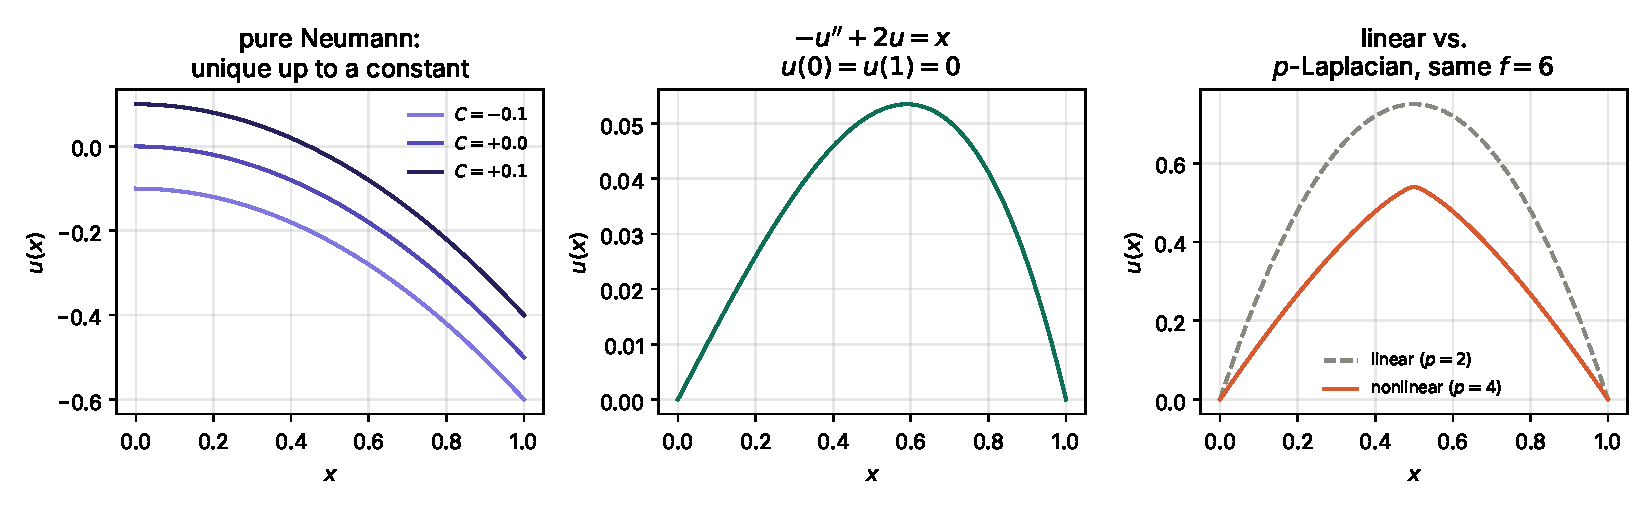
\includegraphics[width=\textwidth]{figures/ch1/ex8_9_10_profiles.pdf}
\caption{Solutions of Exercises~\ref{exo:neumann}--\ref{exo:plaplace}. Left:
the pure Neumann problem is determined up to a constant. Middle: the
reaction--diffusion solution. Right: the nonlinear $p=4$ solution against the
linear $p=2$ solution for the same load $f=6$.}
\label{fig:profiles}
\end{figure}

\paragraph{Guessing the energy from a weak form.}

\exercise{Reconstruct the energy}\label{exo:guess-energy}
\index{energy!from a weak form}%
Find $J$ whose first variation is the weak form: find $u\in H^1(\Omega)$ with
\[
  \int_\Omega\kappa\nabla u\cdot\nabla v\dd x+\int_\Omega\sigma uv\dd x
  =\int_\Omega fv\dd x+\int_{\partial\Omega}gv\dd s\qquad\forall v\in H^1(\Omega),
\]
$\kappa,\sigma>0$ constants.
\begin{solution}
If $a(u,v)=L(v)$ with $a$ \textbf{symmetric} bilinear and $L$ linear, then
$J(u)=\tfrac12a(u,u)-L(u)$ has $\delta J(u)[v]=\tfrac12\bigl(a(u,v)+a(v,u)\bigr)-L(v)=a(u,v)-L(v)$.
Here $a$ is symmetric, so
\[
  J(u)=\tfrac12\int_\Omega\kappa|\nabla u|^2+\tfrac12\int_\Omega\sigma u^2
  -\int_\Omega fu-\int_{\partial\Omega}gu .
\]
\end{solution}

\exercise{When no energy exists}\label{exo:no-energy}
\index{energy!non-existence}%
For the convection--diffusion weak form
$\int_\Omega\nabla u\cdot\nabla v+\int_\Omega(\vb\cdot\nabla u)v=\int_\Omega fv$
on $H^1_0(\Omega)$, $\vb\neq\vzero$ constant, is there an energy $J$ with
$\delta J(u)[v]=a(u,v)-L(v)$?
\begin{solution}
If $J$ existed, its second derivative $a$ would be symmetric (Schwarz's
theorem on mixed derivatives). But for $u,v\in H^1_0$ and constant $\vb$,
integration by parts gives
$\int_\Omega(\vb\cdot\nabla u)v=-\int_\Omega(\vb\cdot\nabla v)u$: the convection
part is \emph{anti}symmetric, so $a(u,v)\neq a(v,u)$ in general. No energy
exists, while Lax--Milgram applies (Section~\ref{sec:var-elliptic}). In 1D
with $b=3$, $u=\sin\pi x$, $v=\sin2\pi x$: $a(u,v)=4$, $a(v,u)=-4$. The skew
part vanishes only on the diagonal $a(u,u)$ (Exercise~\ref{exo:skew}).
\end{solution}

\paragraph{Integration by parts in practice.}

\exercise{Self-adjointness}\label{exo:selfadj}
\index{self-adjointness}%
Let $u,v\in H^2(\Omega)\cap H^1_0(\Omega)$. Use Green's second identity to show
$\int_\Omega u\Delta v=\int_\Omega v\Delta u$.
\begin{solution}
Theorem~\ref{thm:green2} gives
$\int_\Omega(u\Delta v-v\Delta u)=\int_{\partial\Omega}(u\partial_nv-v\partial_nu)$,
and every boundary term contains a vanishing factor $u$ or $v$. This
self-adjointness of the Dirichlet Laplacian is what makes $a(u,v)$ symmetric
and the minimization approach possible.
\end{solution}

\exercise{The Robin problem}\label{exo:robin}
\index{boundary condition!Robin}%
Derive the weak form of $-\Delta u=f$ in $\Omega$, $\partial_nu+\alpha u=g$ on
$\partial\Omega$ ($\alpha>0$), and its energy.
\begin{solution}
Multiply by $v\in H^1(\Omega)$ (Robin, like Neumann, is natural) and use
Green's first identity:
$\int_\Omega\nabla u\cdot\nabla v-\int_{\partial\Omega}\partial_nu\,v=\int_\Omega fv$.
Substituting $\partial_nu=g-\alpha u$:
\[
  \int_\Omega\nabla u\cdot\nabla v+\alpha\int_{\partial\Omega}uv
  =\int_\Omega fv+\int_{\partial\Omega}gv\qquad\forall v\in H^1(\Omega).
\]
The form is symmetric, so
$J(u)=\tfrac12\int_\Omega|\nabla u|^2+\tfrac\alpha2\int_{\partial\Omega}u^2-\int_\Omega fu-\int_{\partial\Omega}gu$.
The Robin condition adds a boundary ``spring'' term, between Dirichlet
($\alpha\to\infty$) and Neumann ($\alpha=0$).
\end{solution}

\exercise{Dirichlet energy from boundary data}\label{exo:dirichlet-energy}
Let $\Delta u=0$ in $\Omega$. Show that
$\int_\Omega|\nabla u|^2=\int_{\partial\Omega}u\,\partial_nu$, and check it on
$(0,1)^3$ for $u=x^2+y^2-2z^2$.
\begin{solution}
Take $v=u$ in Green's first identity; the volume term $\int u\Delta u$
vanishes. The energy of a harmonic field is determined by its boundary data:
this identity is used to compute capacities, and in Chapter~\ref{ch:rg} the
same idea turns boundary measurements into information on a crack. For
$u=x^2+y^2-2z^2$: $\int|\nabla u|^2=\int(4x^2+4y^2+16z^2)=8$; on the boundary, the faces
$x=1$, $y=1$, $z=1$ give $\tfrac43$, $\tfrac43$, $\tfrac{16}3$ and the others $0$: total $8$.
\end{solution}

\framesub{Part III: constraints and convex conjugates}

\exercise{An equality constraint}\label{exo:kkt1}
Minimize $C(\vx)=\tfrac12(x_1^2+x_2^2)$ subject to $x_1-x_2=1$.
\begin{solution}
$\mathcal L=\tfrac12(x_1^2+x_2^2)+\lambda(x_1-x_2-1)$. Stationarity:
$x_1+\lambda=0$, $x_2-\lambda=0$; the constraint gives $-2\lambda=1$. Hence
$\lambda=-\tfrac12$, $\vx=(\tfrac12,-\tfrac12)$, $C=\tfrac14$: the point of the
line closest to the origin.
\end{solution}

\exercise{Two constraints}\label{exo:kkt2}
Minimize $C(\vx)=\tfrac12|\vx|^2$ in $\R^3$ subject to $x_1-x_2=1$ and
$x_2-x_3=2$.
\begin{solution}
Write the constraints $\mat{P}\vx=\vb$ with
$\mat{P}=\begin{psmallmatrix}1&-1&0\\0&1&-1\end{psmallmatrix}$, $\vb=(1,2)$.
Stationarity gives $\vx=-\mat{P}\T\vlambda$, and the constraints
$-\mat{P}\mat{P}\T\vlambda=\vb$ with
$\mat{P}\mat{P}\T=\begin{psmallmatrix}2&-1\\-1&2\end{psmallmatrix}$. Hence
$\vlambda=-(\tfrac43,\tfrac53)$ and $\vx=(\tfrac43,\tfrac13,-\tfrac53)$;
check: $x_1-x_2=1$, $x_2-x_3=2$.
\end{solution}

\exercise{A quadratic form on the circle}\label{exo:kkt3}
\index{eigenvalue problem!as constrained minimization}%
Minimize $C(\vx)=ax_1^2+2bx_1x_2+cx_2^2$ subject to $x_1^2+x_2^2=1$.
\begin{solution}
With $\mat{H}=\begin{psmallmatrix}a&b\\b&c\end{psmallmatrix}$,
$\mathcal L=\vx\T\mat{H}\vx-\lambda(|\vx|^2-1)$ gives $\mat{H}\vx=\lambda\vx$:
the stationary points are the unit eigenvectors, and $C=\lambda$ there. The
minimum is the smallest eigenvalue,
$\tfrac{a+c}2-\sqrt{\bigl(\tfrac{a-c}2\bigr)^2+b^2}$. Constrained minimization
of a quadratic form is an eigenvalue problem: this is the root of the
Rayleigh quotient, of~\eqref{eq:rayleigh}, and of the buckling problems later
in the course.
\end{solution}

\exercise{The saddle-point system}\label{exo:kkt4}
\index{saddle point!system}%
Minimize $C(\vx)=\tfrac12\vx\T\mat{H}\vx-\vx\T\vf$, $\mat{H}$ symmetric
positive definite, subject to $\mat{P}\vx=\vb$ ($\mat{P}$ of full row rank).
\begin{solution}
$\mathcal L=C(\vx)+\vlambda\cdot(\mat{P}\vx-\vb)$, and stationarity in
$(\vx,\vlambda)$ gives
\[
  \begin{bmatrix}\mat{H}&\mat{P}\T\\ \mat{P}&\mat{0}\end{bmatrix}
  \begin{bmatrix}\vx\\ \vlambda\end{bmatrix}=
  \begin{bmatrix}\vf\\ \vb\end{bmatrix},
  \qquad
  \vlambda=(\mat{P}\mat{H}^{-1}\mat{P}\T)^{-1}(\mat{P}\mat{H}^{-1}\vf-\vb),\quad
  \vx=\mat{H}^{-1}(\vf-\mat{P}\T\vlambda).
\]
The matrix is symmetric but indefinite: $(\vx,\vlambda)$ is a saddle point,
a minimum in $\vx$ and a maximum in $\vlambda$. This is the system used for
imposed displacements in Chapter~\ref{ch:elliptic}.
\end{solution}

\exercise{Legendre--Fenchel transforms}\label{exo:lf}
(a) Give a geometric interpretation of $F^\ast$ in $\R^2$ and prove the
Fenchel--Young inequality. (b) Compute $F^\ast$ for $F(x)=x^2$, $F(x)=x^4$,
$F(x)=e^x$, and the indicator $F(x)=0$ for $x\le0$, $+\infty$ for $x>0$.
\begin{solution}
(a) $F^\ast(p)$ is the largest gap between the line $px$ and the graph of
$F$; the line $px-F^\ast(p)$ is the supporting line of slope $p$
(Figure~\ref{fig:legendre}). By definition $F^\ast(p)\ge px-F(x)$ for every
$x$, which is Fenchel--Young; equality holds where the supremum is attained,
$p=F'(x)$.
(b) $x^2$: the maximum of $px-x^2$ is at $x=p/2$, $F^\ast(p)=p^2/4$.
$x^4$: $p=4x^3$, $F^\ast(p)=3(p/4)^{4/3}$.
$e^x$: $F^\ast(p)=p\ln p-p$ for $p>0$, $0$ for $p=0$, $+\infty$ for $p<0$.
Indicator of $\{x\le0\}$: $F^\ast(p)=\sup_{x\le0}px$, which is $0$ for $p\ge0$
and $+\infty$ for $p<0$, the indicator of $\{p\ge0\}$. This last pair is the
convex-analysis form of the complementarity conditions of
Section~\ref{sec:var-lagrange}, and reappears in plasticity.
\end{solution}

%======================================================================
\begin{chapterbib}{99}
\bibitem{AdamsFournier2003} R.~A.~Adams, J.~J.~F.~Fournier, \emph{Sobolev Spaces}, 2nd ed., Academic Press, 2003.
\bibitem{AllenCahn1979} S.~M.~Allen, J.~W.~Cahn, A microscopic theory for antiphase boundary motion and its application to antiphase domain coarsening, \emph{Acta Metall.} 27 (1979) 1085--1095.
\bibitem{BrennerScott2008} S.~C.~Brenner, L.~R.~Scott, \emph{The Mathematical Theory of Finite Element Methods}, 3rd ed., Springer, 2008.
\bibitem{Brezis2011} H.~Brezis, \emph{Functional Analysis, Sobolev Spaces and Partial Differential Equations}, Springer, 2011.
\bibitem{Cea1964} J.~C\'ea, Approximation variationnelle des probl\`emes aux limites, \emph{Ann. Inst. Fourier} 14 (1964) 345--444.
\bibitem{Ciarlet2002} P.~G.~Ciarlet, \emph{The Finite Element Method for Elliptic Problems}, SIAM Classics in Applied Mathematics 40, 2002.
\bibitem{Courant1950} R.~Courant, \emph{Dirichlet's Principle, Conformal Mapping, and Minimal Surfaces}, Interscience, 1950.
\bibitem{Dacorogna2008} B.~Dacorogna, \emph{Direct Methods in the Calculus of Variations}, 2nd ed., Springer, 2008.
\bibitem{EkelandTemam1999} I.~Ekeland, R.~Temam, \emph{Convex Analysis and Variational Problems}, SIAM Classics in Applied Mathematics 28, 1999.
\bibitem{Evans2010} L.~C.~Evans, \emph{Partial Differential Equations}, 2nd ed., AMS, 2010.
\bibitem{Garding1953} L.~G\aa rding, Dirichlet's problem for linear elliptic partial differential equations, \emph{Math. Scand.} 1 (1953) 55--72.
\bibitem{GilbargTrudinger2001} D.~Gilbarg, N.~S.~Trudinger, \emph{Elliptic Partial Differential Equations of Second Order}, Springer Classics in Mathematics, 2001.
\bibitem{LaxMilgram1954} P.~D.~Lax, A.~N.~Milgram, Parabolic equations, in \emph{Contributions to the Theory of Partial Differential Equations}, Ann. Math. Studies 33, Princeton, 1954, 167--190.
\bibitem{Rockafellar1970} R.~T.~Rockafellar, \emph{Convex Analysis}, Princeton University Press, 1970.
\bibitem{Strang1986} G.~Strang, \emph{Introduction to Applied Mathematics}, Wellesley-Cambridge Press, 1986.
\end{chapterbib}

%======================================================================
\chapter{Elliptic problems: diffusion and elasticity}\label{ch:elliptic}
%======================================================================
% Sources: lecture notes C1 (Section 3), slides L01 "Elasticity" (2025)
% and L02 "Elasticity, constraints, Lagrangian".

\framepart{Outline}
The two model problems of continuum mechanics treated in this chapter, steady
diffusion and linear elasticity, share the structure found in
Chapter~\ref{ch:var} for a chain of springs: a kinematic operator, a
constitutive law, and an equilibrium operator which is the adjoint of the
kinematic one. The scalar problem (diffusion) is the template; elasticity is
its vector--tensor version. For both we state the equations, the weak form,
the two energy principles, and the approximation by the Ritz--Galerkin and
finite element methods.

\paragraph{By the end of this chapter you should be able to:}
\begin{itemize}
  \item write the strong form, the weak form and the energies of a diffusion
  or a linear elasticity problem, with its essential and natural boundary
  conditions;
  \item handle the tensor of diffusion coefficients $\tk$ and the tensor of
  elastic moduli $\bbC$: their symmetries, their matrix representation,
  isotropy and the conditions of positive definiteness;
  \item read the structure of both problems on their Tonti diagram, with the
  adjoint operators $\nabla$ and $-\dive$, $\eps[\cdot]$ and $-\dive$, and the
  boundary traces $\cdot\,\vn$;
  \item write the Lagrangian of the potential energy, with thermal terms and
  boundary conditions, and derive all the equations from it;
  \item state and prove the minimum of the potential energy and the maximum
  of the complementary energy, and use them to bound the solution;
  \item build a Ritz--Galerkin approximation, impose displacements with
  Lagrange multipliers, and recognize the finite element method as a
  particular case.
\end{itemize}

\paragraph{Plan of the chapter.} Section~\ref{sec:diff} treats steady diffusion.
Sections~\ref{sec:el-eq}--\ref{sec:el-moduli} state the equations of linear
elasticity and discuss the elastic moduli. Section~\ref{sec:el-structure}
displays the common structure of the equations, Section~\ref{sec:el-vw} the
principle of virtual work and Section~\ref{sec:el-energy} the energy
principles. Section~\ref{sec:el-ritz} presents approximate solutions, from
Ritz--Galerkin to finite elements. A summary, exercises with solutions
(page~\pageref{sec:el-exo}) and the references close the chapter. Classical references for the mechanics are
\cite{Germain1983,Salencon2001,Coirier1997,SoutasLittle1973,ConstantinescuKorsunsky2007};
for the structure of the equations \cite{StrangAM}; for finite elements
\cite{Hughes1987,BonnetFrangi2007}.

\begin{table}[h]
\centering\small
\renewcommand{\arraystretch}{1.2}
\begin{tabular}{lll}
\toprule
 & \sffamily diffusion & \sffamily elasticity\\
\midrule
primary unknown & potential $u$ (scalar) & displacement $\vu$ (vector)\\
kinematic field & gradient $\nabla u$ & strain $\eps=\tfrac12(\nabla\vu+\nabla\vu\T)$\\
material law & conductivity $\tk$ (2nd order) & elastic moduli $\bbC$ (4th order)\\
static field & flux $\tk\nabla u$ (vector) & stress $\sig=\bbC:\eps$ (2nd order)\\
equilibrium & $\dive(\tk\nabla u)+f=0$ & $\dive\sig+\vf=\vzero$\\
essential data on $S_u$ & $u=\uD$ & $\vu=\vuD$\\
natural data on $S_\varphi$, $S_t$ & $(\tk\nabla u)\cdot\vn=\pD$ & $\sig\vn=\vtD$\\
energy density & $\tfrac12\nabla u\cdot\tk\nabla u$ & $\tfrac12\eps:\bbC:\eps$\\
\bottomrule
\end{tabular}
\caption{The two elliptic model problems side by side.}
\label{tab:diff-el}
\end{table}

%======================================================================
\section{Steady diffusion}\label{sec:diff}
\index{diffusion}\index{conductivity tensor}\index{boundary condition!essential}\index{boundary condition!natural}%
A potential $u$ (temperature, electric potential, hydraulic head,
concentration, out-of-plane displacement) drives a flux. The section follows
the same frame as elasticity: the equations, the coefficients, the structure,
virtual power, the energy principles and the Lagrangian.

\subsection{The equations}
\begin{gbox}{Diffusion problem}
Let $\Omega\subset\R^3$ be a bounded Lipschitz domain with outward unit normal
$\vn$, and $\partial\Omega=\overline{S_u}\cup\overline{S_\varphi}$,
$S_u\cap S_\varphi=\emptyset$, a partition of its boundary. Find the potential
$u$ and the flux $\vp$ such that
\begin{align}
  \vp&=\tk\nabla u &&\text{constitutive law (Fourier, Ohm, Darcy, Fick)},\label{eq:diff-law}\\
  \dive\vp+f&=0 &&\text{balance in }\Omega,\label{eq:diff-balance}\\
  u=\uD\ \text{on }S_u, &\qquad \vp\cdot\vn=\pD\ \text{on }S_\varphi
  &&\text{boundary conditions}.\label{eq:diff-bc}
\end{align}
Eliminating the flux,
\begin{equation}\label{eq:diffusion}
\left\{\begin{aligned}
\dive(\tk\nabla u)+f&=0 &&\text{in }\Omega,\\
u&=\uD &&\text{on }S_u \quad\text{(potential given)},\\
(\tk\nabla u)\cdot\vn&=\pD &&\text{on }S_\varphi \quad\text{(flux given)}.
\end{aligned}\right.
\end{equation}
In components: $p_i=k_{ij}u_{,j}$, $p_{i,i}+f=0$, $p_in_i=\pD$.
\end{gbox}
The physical flux is $\vq=-\vp=-\tk\nabla u$: heat flows from hot to cold,
and $\pD=-\vq\cdot\vn$ is the \emph{incoming} flux; $f$ is a volume source.

\subsection{The tensor of diffusion coefficients}
\index{conductivity tensor!symmetry and positivity}%
\begin{gbox}{Symmetry and positivity of $\tk$}
\begin{itemize}
  \item $\tk=k_{ij}\,\ve_i\otimes\ve_j$ is a second-order tensor field;
  \item symmetry, $k_{ij}=k_{ji}$: condition for an energy to exist (as for the
  springs, Section~\ref{ssec:symmetry}); in thermodynamics, Onsager's
  reciprocity;
  \item positivity, $\vxi\cdot\tk\vxi\ge\alpha|\vxi|^2$ with $\alpha>0$: positive
  dissipation, heat flows from hot to cold;
  \item isotropy: $\tk=k\,\tI$ with $k>0$, a single coefficient.
\end{itemize}
\end{gbox}
In its principal axes $\tk=\diag(k_1,k_2,k_3)$, $k_i>0$: isotropic for
$k_1=k_2=k_3=k$, transversely isotropic for a fibre composite or a layered
rock, $k_1=k_2\neq k_3$. It is the second-order counterpart of the fourth-order
tensor $\bbC$ of elasticity (Section~\ref{sec:el-moduli}). In the rest of this
section the medium is isotropic, and Table~\ref{tab:diff-values} gives orders
of magnitude of $k$ in the physical settings of the model problem.

\begin{table}[h]
\centering\small
\renewcommand{\arraystretch}{1.18}
\begin{tabular}{>{\raggedright}p{2.5cm}>{\raggedright}p{2.6cm}>{\raggedright}p{3.0cm}>{\raggedright\arraybackslash}p{6.2cm}}
\toprule
\sffamily setting & \sffamily potential $u$ & \sffamily coefficient $k$ & \sffamily typical values (room temperature)\\
\midrule
heat conduction (Fourier) & temperature [K] & thermal conductivity [W\,m$^{-1}$K$^{-1}$] &
copper 400, aluminium 237, carbon steel 50, stainless steel 15, concrete 1--2, glass 1, water 0.6, wood 0.1--0.2, polymer foam 0.03, air 0.026\\
electric conduction (Ohm) & electric potential [V] & electrical conductivity [S\,m$^{-1}$] &
copper $6.0\times10^{7}$, aluminium $3.8\times10^{7}$, carbon steel $\approx6\times10^{6}$, stainless steel $1.4\times10^{6}$, sea water 5, tap water $10^{-3}$--$10^{-1}$, glass $10^{-15}$--$10^{-11}$\\
porous media (Darcy) & hydraulic head [m] & hydraulic conductivity [m\,s$^{-1}$] &
gravel $10^{-3}$--$1$, clean sand $10^{-5}$--$10^{-2}$, silt $10^{-9}$--$10^{-5}$, clay $10^{-12}$--$10^{-9}$\\
mass diffusion (Fick) & concentration [mol\,m$^{-3}$] & diffusion coefficient [m$^2$\,s$^{-1}$] &
gases in air $\approx2\times10^{-5}$ (CO$_2$: $1.6\times10^{-5}$), small solutes in water $\approx10^{-9}$ (NaCl: $1.6\times10^{-9}$), carbon in austenite at $1000^\circ$C $\approx3\times10^{-11}$\\
anti-plane elasticity & displacement $u_3$ [m] & shear modulus $\mu$ [Pa] &
steel $80\times10^{9}$, copper $45\times10^{9}$, aluminium $26\times10^{9}$, rubber $\approx10^{6}$\\
\bottomrule
\end{tabular}
\caption{Isotropic diffusion coefficients $k$ in the settings of the model
problem $\dive(k\nabla u)+f=0$. Orders of magnitude; values depend on
composition and temperature~\cite{IncroperaDeWitt,FreezeCherry,Crank1975}.}
\label{tab:diff-values}
\end{table}
The ranges are striking: thermal conductivities span four orders of
magnitude, electrical conductivities more than twenty, hydraulic
conductivities twelve. The same equation therefore describes a copper bar
(a good conductor, almost uniform potential) and a clay barrier (a nearly
impermeable one); only the ratio of $k$ between neighbouring materials
matters for the shape of the field, and an insulating crack is the limit
$k\to0$ in a thin layer (Chapter~\ref{ch:rg}).

\subsection{Structure of the equations}
\index{Tonti diagram!diffusion}\index{admissible fields!diffusion}%
The diffusion problem has the structure of the spring chain of
Chapter~\ref{ch:var} (Figure~\ref{fig:tonti-diff}): the gradient plays the
role of $\mat{B}$, the conductivity that of $\mat{C}$, and the pair formed by
$-\dive$ in $\Omega$ and the normal trace $\cdot\,\vn$ on $S_\varphi$ that of
$\mat{B}\T$. Substituting, $u$ solves $-\dive(\tk\nabla u)=f$; for an isotropic
homogeneous medium, $\tk=k\tI$, this is the Poisson equation $-k\Delta u=f$.
\begin{figure}[h]
\centering
\begin{tikzpicture}[node distance=1.2cm and 1.3cm,
  tb/.style={smallbox,minimum width=4.3cm}]
  \node[tb,kin] (u) {$u$, \quad $u=\uD$ on $S_u$\\ \footnotesize potential};
  \node[tb,stat,right=3.6cm of u] (f) {$\dive\vp+f=0$ in $\Omega$,\ \ $\vp\cdot\vn=\pD$ on $S_\varphi$\\ \footnotesize sources and boundary fluxes};
  \node[tb,kin,below=of u] (e) {$\nabla u$\\ \footnotesize gradient};
  \node[tb,stat,below=of f] (s) {$\vp=\tk\nabla u$\\ \footnotesize flux};
  \draw[arr] (u) -- (e) node[midway,left,font=\small]{$\nabla$};
  \draw[arr] (e) -- (s) node[midway,below,font=\small]{$\tk$};
  \draw[arr] (s) -- (f) node[midway,right,font=\small]{$-\dive$, \ $\cdot\,\vn$};
  \node[below=0.15cm of e,kinlab,align=center] {kinematically admissible: $\Kad(\uD,S_u)$};
  \node[below=0.15cm of s,statlab,align=center] {statically admissible: $\Sad(f,\pD,S_\varphi)$};
\end{tikzpicture}
\caption{Tonti diagram of steady diffusion. Left column (blue): kinematic
quantities, with the potential prescribed on $S_u$; right column (green):
static quantities, with the balance of the flux and the prescribed boundary
flux. Compare with Figures~\ref{fig:tonti-discrete} and~\ref{fig:tonti-el}.}
\label{fig:tonti-diff}
\end{figure}
The two columns define the two sets of admissible fields:
\begin{align*}
  \Kad(\uD,S_u)&=\{v\ :\ v=\uD\ \text{on }S_u\},\\
  \Sad(f,\pD,S_\varphi)&=\{\vp\ :\ \dive\vp+f=0\ \text{in }\Omega,\ \vp\cdot\vn=\pD\ \text{on }S_\varphi\}.
\end{align*}
The solution is the potential $u\in\Kad$ whose flux $\tk\nabla u$ lies in
$\Sad$.

\subsection{Virtual power: the weak form of the balance}
\index{virtual power principle!diffusion}\index{weak form!diffusion}%
For a virtual potential $v$ define the virtual powers of the sources and of
the fluxes:
\[
  \mathcal P_e(v)=\int_\Omega fv\dd x+\int_{\partial\Omega}(\vp\cdot\vn)\,v\dd s,\qquad
  \mathcal P_i(v)=-\int_\Omega\vp\cdot\nabla v\dd x .
\]
\begin{gbox}{Principle of virtual power (diffusion)}
For every virtual potential $v$,
\begin{equation}\label{eq:diff-pvp}
  \mathcal P_e(v)+\mathcal P_i(v)=0 .
\end{equation}
For a uniform field $v=c$, $\nabla v=\vzero$ and $\mathcal P_i(v)=0$: the
constants play the role of rigid motions.
\end{gbox}
The principle is equivalent to the balance~\eqref{eq:diff-balance} and to the
boundary flux $\vp\cdot\vn$. Indeed, by Theorem~\ref{thm:ibp-matrix},
\[
  \int_\Omega\vp\cdot\nabla v\dd x=-\int_\Omega(\dive\vp)\,v\dd x
  +\int_{\partial\Omega}(\vp\cdot\vn)\,v\dd s ,
\]
and~\eqref{eq:diff-pvp} for all $v$ is $\displaystyle \int_\Omega(\dive\vp+f)\,v\dd x=0$.
Choosing $v=1$ gives the global balance $\displaystyle \int_\Omega f\dd x+\int_{\partial\Omega}\vp\cdot\vn\dd s=0$:
what is produced inside leaves through the boundary.

With the constitutive law, and $v$ restricted to the fields vanishing on
$S_u$, the principle becomes the weak form of diffusion: find
$u\in\Kad(\uD,S_u)$ such that
\begin{equation}\label{eq:diffusion-weak}
  \int_\Omega\tk\nabla u\cdot\nabla v\dd x=\int_\Omega fv\dd x
  +\int_{S_\varphi}\pD v\dd s\qquad\forall v\in\Kad(0,S_u).
\end{equation}
If $|S_u|>0$, the Poincar\'e inequality holds on $\Kad(0,S_u)$, the form is
coercive, and Lax--Milgram gives a unique solution depending continuously on
the data: the problem is well posed. If $S_u=\emptyset$, a solution exists only
if $\displaystyle \int_\Omega f+\int_{\partial\Omega}\pD=0$ (the global balance above),
and it is unique up to a constant (Exercise~\ref{exo:neumann}).

\subsection{Energy principles}
\index{energy!potential (diffusion)}\index{energy!complementary (diffusion)}%
As in thermoelasticity (Section~\ref{sec:el-energy}), we include an
\emph{initial flux} $\vp_0$ and an \emph{imposed gradient} $\vect{g}^D$, so that
\[
  \vp=\vp_0+\tk\,(\nabla u-\vect{g}^D).
\]
In porous media written in pressure, $\vect{g}^D=\rho\vect{g}$ is the weight of the
fluid (gravity drives the flow even without pressure gradient); $\vp_0$
represents a prescribed background flux. Without them, $\vp=\tk\nabla u$.

\begin{gbox}{Potential energy (diffusion)}
For $v\in\Kad(\uD,S_u)$,
\begin{equation}\label{eq:diffusion-energy}
  J(v)=\int_\Omega\Bigl(\vp_0\cdot\nabla v
  +\tfrac12(\nabla v-\vect{g}^D)\cdot\tk(\nabla v-\vect{g}^D)\Bigr)\dd x
  -\int_\Omega fv\dd x-\int_{S_\varphi}\pD v\dd s .
\end{equation}
\end{gbox}

\begin{gbox}{Complementary energy (diffusion)}
For $\vq\in\Sad(f,\pD,S_\varphi)$, with $\hat\vq=\vq-\vp_0+\tk\vect{g}^D$,
\begin{equation}\label{eq:diffusion-comp}
  J^\ast(\vq)=-\frac12\int_\Omega\hat\vq\cdot\tk^{-1}\hat\vq\dd x
  +\int_{S_u}\uD\,(\vq\cdot\vn)\dd s .
\end{equation}
\end{gbox}

\begin{gbox}{Extremal properties (diffusion)}
Let $(u,\vp)$ be the solution.
\begin{itemize}
\item $u$ \emph{minimizes} the potential energy over the kinematically
admissible potentials: $J(v)\ge J(u)$ for all $v\in\Kad(\uD,S_u)$.
\item $\vp$ \emph{maximizes} the complementary energy over the statically
admissible fluxes: $J^\ast(\vp)\ge J^\ast(\vq)$ for all $\vq\in\Sad(f,\pD,S_\varphi)$.
\item If $\vp_0=\vzero$ and $\vect{g}^D=\vzero$, the two values coincide:
$J(u)=J^\ast(\vp)$.
\end{itemize}
\end{gbox}
For any admissible pair,
$J^\ast(\vq)\le J^\ast(\vp)=J(u)\le J(v)$: two-sided bounds, as in elasticity.
The proof is the same as for elasticity (Section~\ref{sec:el-energy}): the
weak form~\eqref{eq:diffusion-weak} kills the linear part of $J(v)-J(u)$, and
the quadratic part $\tfrac12\int\nabla(v-u)\cdot\tk\nabla(v-u)$ is non-negative.
The gap $J(v)-J^\ast(\vq)$ is computed in Exercise~\ref{exo:diff-comp}.

\subsection{The Lagrangian of the potential energy}\label{ssec:diff-lagrangian}
\index{Lagrangian!diffusion}\index{Lagrange multiplier!boundary flux}%
As for elasticity (Section~\ref{ssec:el-lagrangian}), the constraint
$u=\uD$ on $S_u$ is relaxed with a Lagrange multiplier on $S_u$, which yields
all the equations, including the boundary conditions and the reactions, from
a single stationarity condition~\cite{BonnetFrangi2007}.

\begin{gbox}{Lagrangian of diffusion}
For unconstrained potentials $v$ and multipliers $\mu$ on $S_u$,
\begin{multline}\label{eq:L-diff}
  \mathcal L(v,\mu)=\int_\Omega\Bigl(\vp_0\cdot\nabla v
  +\tfrac12(\nabla v-\vect{g}^D)\cdot\tk(\nabla v-\vect{g}^D)\Bigr)\dd x\\
  -\int_\Omega fv\dd x-\int_{S_\varphi}\pD v\dd s
  -\int_{S_u}\mu\,(v-\uD)\dd s .
\end{multline}
The solution $(u,\mu)$ is a saddle point of $\mathcal L$: a minimum in $v$ and
a maximum in $\mu$.
\end{gbox}
\paragraph{Derivation of the equations.} Write
$\vp=\vp_0+\tk(\nabla u-\vect{g}^D)$. Stationarity with respect to $\mu$ gives
$u=\uD$ on $S_u$. Stationarity with respect to $v$, in every direction $w$,
gives
\[
  \int_\Omega\vp\cdot\nabla w\dd x-\int_\Omega fw\dd x
  -\int_{S_\varphi}\pD w\dd s-\int_{S_u}\mu\,w\dd s=0 .
\]
Integrating by parts with Theorem~\ref{thm:ibp-matrix},
\[
  \int_\Omega(-\dive\vp-f)\,w\dd x+\int_{S_\varphi}(\vp\cdot\vn-\pD)\,w\dd s
  +\int_{S_u}(\vp\cdot\vn-\mu)\,w\dd s=0\qquad\forall w,
\]
hence the balance $\dive\vp+f=0$ in $\Omega$, the flux condition
$\vp\cdot\vn=\pD$ on $S_\varphi$, and $\mu=\vp\cdot\vn$ on $S_u$: the multiplier
is the incoming flux through the boundary where the potential is imposed, the
``reaction'' of diffusion, for instance the heat supplied by a thermostat or
the current through an electrode. The constitutive law, with its initial flux and imposed gradient,
is contained in the definition of the energy density.

\paragraph{Remarks.}
\begin{itemize}
  \item \emph{Essential and natural conditions.} The potential $\uD$ is built
  into the space $\Kad$ or imposed by the multiplier; the flux $\pD$ appears as
  a boundary term of the energy. In a finite element code, the first are
  imposed on the unknowns or by Lagrange multipliers
  (Section~\ref{ssec:ritz-lagrange}), the second enter the right-hand side.
  \item \emph{Complementary boundary conditions.} On each part of the
  boundary exactly one datum is given, potential or flux. If both are known
  on a part of the boundary and nothing on another, the problem is no longer
  a direct problem: it becomes an \emph{inverse problem}, which is the subject
  of Chapter~\ref{ch:rg}.
\end{itemize}

%======================================================================
\section{Linear elasticity: the equations}\label{sec:el-eq}
\index{elasticity!equations}\index{strain}\index{stress}\index{Hooke's law}%
\begin{figure}[h]
\centering
\begin{tikzpicture}[scale=1.0,>={Latex[length=2mm]},
  hatch/.style={postaction={decorate},decoration={markings,
    mark=between positions 0.02 and 0.98 step 5pt with {\draw[cu!70,thin] (0,0) -- (-3pt,-5pt);}}}]
  \coordinate (A) at (0,0.6);
  \coordinate (B) at (2.0,-0.4);
  \coordinate (C) at (4.4,0.5);
  \coordinate (D) at (3.9,2.6);
  \coordinate (E) at (1.0,2.5);
  \fill[gray!12] (A) to[out=-70,in=180] (B) to[out=0,in=-130] (C)
    to[out=50,in=-30] (D) to[out=150,in=10] (E) to[out=190,in=110] (A);
  % S_u: displacement given (kinematic data, blue), hatched support
  \draw[cu,very thick,hatch] (E) to[out=190,in=110] (A) to[out=-70,in=180] (B);
  % S_t: traction given (static data, green), tractions and normal
  \draw[cphi,very thick,postaction={decorate},decoration={markings,
     mark=at position 0.16 with {\draw[->,thick,cphi] (0,0) -- (0.35,-0.75);},
     mark=at position 0.40 with {\draw[->,thick,cphi] (0,0) -- (-0.25,-0.8);},
     mark=at position 0.62 with {\draw[->,thick,cphi] (0,0) -- (0.3,-0.75) coordinate (T);},
     mark=at position 0.82 with {\draw[->,thick] (0,0) -- (0,-0.8) coordinate (N);}}]
    (B) to[out=0,in=-130] (C) to[out=50,in=-30] (D) to[out=150,in=10] (E);
  \node[cphi,above right,inner sep=1pt] at (T) {$\vt=\vtD$};
  \node[left] at (N) {$\vn$};
  \draw[->,thick] (2.6,1.5) -- (2.6,0.75) node[right] {$\vf$};
  \node at (1.6,1.3) {$\Omega$};
  \node[cu,anchor=east,align=right,font=\small] at (-0.35,1.5) {$S_u$: displacement\\ given, $\vu=\vuD$};
  \node[cphi,anchor=west,align=left,font=\small] at (5.0,1.2) {$S_t$: traction\\ given, $\sig\vn=\vtD$};
\end{tikzpicture}
\caption{A body $\Omega$ under body forces $\vf$. The displacement is given
on $S_u$ (blue, kinematic data); the traction $\vt=\sig\vn$ is given on $S_t$
(green, static data); $\vn$ is the outward unit normal.}
\label{fig:3Dbody}
\end{figure}
A continuous body occupies $\Omega\subset\R^3$, described in Cartesian
coordinates, $\vv=v_1\ve_1+v_2\ve_2+v_3\ve_3$ (Figure~\ref{fig:3Dbody}). The
fields are
\begin{itemize}
  \item the vector field of displacements, $\vu$;
  \item the second-order tensor field of small strains, $\eps$;
  \item the second-order tensor field of stresses, $\sig$;
  \item the vector field of body forces, $\vf$, and of boundary tractions, $\vt$.
\end{itemize}
The equations fall into four groups: \emph{kinematics} (strains),
\emph{constitutive law} (linear elasticity), \emph{balance of forces}
(stresses), and \emph{boundary conditions} (imposed tractions or
displacements). Two equivalent formulations follow: the \emph{virtual work}
(weak form of the balance) and the \emph{energy} principles (minimum and
maximum).

\begin{gbox}{Equations of linear elasticity}
\begin{align}
  \eps&=\tfrac12\bigl(\nabla\vu+\nabla\vu\T\bigr)
  &&\text{kinematics}, \label{eq:kine}\\
  \sig&=\bbC:\eps &&\text{constitutive law (Hooke)}, \label{eq:hooke}\\
  \dive\sig+\vf&=\vzero &&\text{balance (static equilibrium)}, \label{eq:balance}\\
  \vu=\vuD\ \text{on }S_u, &\qquad \sig\vn=\vtD\ \text{on }S_t
  &&\text{boundary conditions}, \label{eq:bc}
\end{align}
with $\partial\Omega=\overline{S_u}\cup\overline{S_t}$, $S_u\cap S_t=\emptyset$.
In components: $\varepsilon_{ij}=\tfrac12(u_{i,j}+u_{j,i})$,
$\sigma_{ij}=C_{ijkl}\varepsilon_{kl}$, $\sigma_{ij,j}+f_i=0$, $\sigma_{ij}n_j=t^D_i$.
\end{gbox}

\paragraph{Classical boundary conditions.} The partition $S_u$/$S_t$ is a
\index{boundary condition!elasticity}\index{contact!frictionless}%
simplification: in general, at each boundary point, three complementary
components are prescribed. With $\vt_1,\vt_2$ two unit tangent vectors:
\begin{itemize}
  \item \emph{clamped} (encastr\'e): $\vu=\vzero$, i.e.\ $u_i=0$ for all $i$;
  \item \emph{traction-free surface}: $\sig\vn=\vzero$, i.e.\ $\sigma_{ij}n_j=0$;
  \item \emph{frictionless sliding contact}: $\vu\cdot\vn=u^D$,
  $\vt_1\cdot\sig\vn=0$, $\vt_2\cdot\sig\vn=0$;
  \item \emph{prescribed pressure and shear}: $\sig\vn=-p\vn+q_1\vt_1+q_2\vt_2$,
  i.e.\ $\vn\cdot\sig\vn=-p$, $\vt_1\cdot\sig\vn=q_1$, $\vt_2\cdot\sig\vn=q_2$.
\end{itemize}

\paragraph{Mixed conditions.}
\index{boundary condition!mixed}%
Sliding contact is the typical \emph{mixed} condition: at the same point, some
components are kinematic data and the complementary ones static data. A plane
of symmetry with normal $\vn$ is of this type: $\vu\cdot\vn=0$ and zero shear
traction. The weak form handles mixed conditions without change: the test
fields $\vv$ satisfy the homogeneous kinematic components only ($\vv\cdot\vn=0$),
and the static components enter the load as natural conditions. The rule
``three complementary components at each point'' is what makes the
boundary-value problem well posed.

%======================================================================
\section{Elastic moduli}\label{sec:el-moduli}
\subsection{The tensor of elastic moduli}
\index{elastic moduli}\index{elastic moduli!symmetries}\index{compliance tensor}%
The constitutive law
\[
  \sig=\bbC:\eps,\qquad \sigma_{ij}=C_{ijkl}\varepsilon_{kl},
  \qquad\text{e.g. }\ \sigma_{23}=C_{2311}\varepsilon_{11}+C_{2312}\varepsilon_{12}
  +C_{2313}\varepsilon_{13}+C_{2321}\varepsilon_{21}+\cdots
\]
involves the fourth-order tensor of elastic moduli
\[
  \bbC=C_{ijkl}\,\ve_i\otimes\ve_j\otimes\ve_k\otimes\ve_l .
\]
\begin{gbox}{Symmetries and positivity of $\bbC$}
\begin{itemize}
  \item symmetry of the strain $\eps$ (minor symmetry): $C_{ijkl}=C_{ijlk}$;
  \item symmetry of the stress $\sig$ (minor symmetry): $C_{ijkl}=C_{jikl}$;
  \item existence of an energy potential (major symmetry): $C_{ijkl}=C_{klij}$,
  i.e.\ $\eps_1:\bbC:\eps_2=\eps_2:\bbC:\eps_1$;
  \item stability (positive definiteness):
  $\eps:\bbC:\eps>0$ and $\sig:\bbS:\sig>0$ for $\eps,\sig\neq\vzero$,
  with $\bbS=\bbC^{-1}$ the compliance tensor.
\end{itemize}
The symmetries leave $21$ independent moduli.
\end{gbox}
The major symmetry is the continuum analogue of the symmetry of $\mat{K}$ in
Section~\ref{ssec:symmetry}: without it the work of deformation would depend
on the path, and no stored energy would exist.

\paragraph{Matrix representation.} With the minor symmetries, stresses and
\index{Voigt notation}\index{Mandel notation}\index{elastic moduli!matrix representation}%
strains have six independent components and $\bbC$ is represented by a
symmetric $6\times6$ matrix:
\begin{equation}\label{eq:voigt}
 \begin{pmatrix}\sigma_{11}\\ \sigma_{22}\\ \sigma_{33}\\ \sigma_{23}\\ \sigma_{31}\\ \sigma_{12}\end{pmatrix}
 =
 \begin{pmatrix}
   C_{1111} & C_{1122} & C_{1133} & C_{1123} & C_{1131} & C_{1112} \\
            & C_{2222} & C_{2233} & C_{2223} & C_{2231} & C_{2212} \\
            &          & C_{3333} & C_{3323} & C_{3331} & C_{3312} \\
            &          &          & C_{2323} & C_{2331} & C_{2312} \\
            & \text{sym.} &       &          & C_{3131} & C_{3112} \\
            &          &          &          &          & C_{1212}
 \end{pmatrix}
 \begin{pmatrix}\varepsilon_{11}\\ \varepsilon_{22}\\ \varepsilon_{33}\\ 2\varepsilon_{23}\\ 2\varepsilon_{31}\\ 2\varepsilon_{12}\end{pmatrix}.
\end{equation}
In \emph{Voigt notation} the entries are renamed $c_{IJ}$, $I,J=1,\dots,6$,
with $11\to1$, $22\to2$, $33\to3$, $23\to4$, $31\to5$, $12\to6$. The factors
$2$ on the shear strains make $\vect{\sigma}\cdot\vect{\varepsilon}$ in
$\R^6$ equal to $\sig:\eps$, but the matrix of $\bbS$ then carries factors
$2$ and $4$; the orthonormal (Mandel) basis, with factors $\sqrt2$, avoids
this asymmetry.

\paragraph{Measured values.} Table~\ref{tab:el-stiffness} gives the elastic
\index{elastic moduli!measured values}%
stiffnesses of crystals at room temperature. They are computed from the
compliances listed by Nye~\cite{Nye1985}: the $6\times6$ compliance matrix
is built with the structure of the symmetry class and inverted
(Exercise~\ref{exo:stiffness}). For cadmium the table gives the measured
adiabatic stiffnesses.
\begin{table}[h]
\centering\small
\renewcommand{\arraystretch}{1.1}
\begin{tabular}{llrrrrrrr}
\toprule
\sffamily crystal & \sffamily symmetry & $c_{11}$ & $c_{12}$ & $c_{13}$ & $c_{33}$ & $c_{44}$ & $c_{66}$ & $c_{14}$\\
\midrule
sodium chloride & cubic      &  51 &  13   &     &     &  13 &     &    \\
aluminium       & cubic      & 108 &  62   &     &     &  28 &     &    \\
copper          & cubic      & 176 & 129   &     &     &  75 &     &    \\
nickel          & cubic      & 250 & 160   &     &     & 118 &     &    \\
tungsten        & cubic      & 502 & 199   &     &     & 152 &     &    \\
tin             & tetragonal &  84 &  49   &  28 &  97 &  18 &   7 &    \\
ADP             & tetragonal &  71 & $-20$ &  13 &  30 &   9 &   6 &    \\
zinc            & hexagonal  & 164 &  27   &  52 &  63 &  38 &     &    \\
cadmium         & hexagonal  & 115 &  40   &  40 &  51 &  20 &     &    \\
quartz          & trigonal   &  87 &   8   &  15 & 108 &  57 &     & 17 \\
tourmaline      & trigonal   & 268 &  66   &   8 & 159 &  67 &     &  8 \\
\bottomrule
\end{tabular}
\caption{Elastic stiffnesses $c_{IJ}$ of crystals at room temperature, in GPa
(Voigt notation, axis $3$ along the main symmetry axis). Blank entries follow
from the symmetry class: cubic, $c_{33}=c_{11}$, $c_{13}=c_{12}$,
$c_{66}=c_{44}$; hexagonal and trigonal, $c_{66}=\tfrac12(c_{11}-c_{12})$;
trigonal, $c_{24}=-c_{14}$, $c_{56}=c_{14}$; all other entries vanish.
Computed from the compliances of~\cite{Nye1985}; cadmium: measured adiabatic
values.}
\label{tab:el-stiffness}
\end{table}
The inversion amplifies the rounding of the compliances. For a cubic crystal
$c_{11}+2c_{12}=1/(s_{11}+2s_{12})=3K$, and $s_{11}+2s_{12}$ is a small
difference of two numbers. The two-digit compliances of copper give $c_{11}$
and $c_{12}$ about $5\%$ above the values measured directly, $168$ and
$121$\,GPa; $c_{44}=1/s_{44}$ is not affected.

\subsection{Anisotropy and isotropy}
\index{anisotropy}\index{elasticity!anisotropic}\index{symmetry classes}%
Depending on its symmetry group, a linear elastic material belongs to one of
eight classes~\cite{Chadwick2001}: triclinic ($21$ moduli), monoclinic
($13$), orthotropic ($9$), trigonal ($6$), tetragonal ($6$), transversely
isotropic ($5$), cubic ($3$) and isotropic ($2$). Hexagonal crystals are
transversely isotropic.

\paragraph{Directional Young's modulus.} The modulus in tension along a unit
\index{Young's modulus!directional}\index{Zener ratio}%
vector $\vd$ is $1/E(\vd)=\vd\otimes\vd:\bbS:\vd\otimes\vd$. For a cubic
crystal,
\[
  \frac{1}{E(\vd)}=s_{11}-2\Bigl(s_{11}-s_{12}-\tfrac12s_{44}\Bigr)
  \bigl(d_1^2d_2^2+d_2^2d_3^2+d_3^2d_1^2\bigr).
\]
The crystal is isotropic iff the Zener ratio $A=2c_{44}/(c_{11}-c_{12})$
equals $1$. Tungsten is almost isotropic ($A=1.0$). Copper is strongly
anisotropic ($A=3.2$): $E=1/s_{11}=67$\,GPa along a cube edge
$\langle100\rangle$ and $E=192$\,GPa along a cube diagonal $\langle111\rangle$. Zinc, a hexagonal crystal, is soft along
its axis, $E=1/s_{33}=35$\,GPa, and stiff across it: $119$\,GPa in the basal
plane, $124$\,GPa at $70^\circ$ from the axis (Figure~\ref{fig:el-young}).

\begin{figure}[h]
\centering
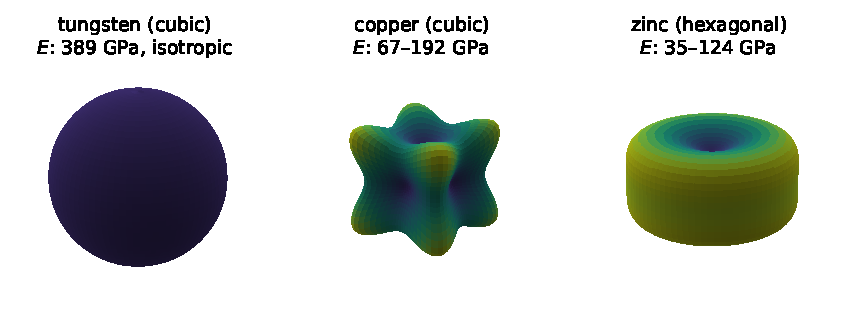
\includegraphics[width=0.92\textwidth]{figures/ch2/young_surface.pdf}
\caption{Directional Young's modulus: the surface $r=E(\vd)\,\vd$, coloured by
$E$ (each panel has its own scale). Tungsten is isotropic within the accuracy
of its compliances; copper is stiffest along the cube diagonals; zinc is
transversely isotropic about its hexagonal axis (vertical). Compliances
of~\cite{Nye1985}.}
\label{fig:el-young}
\end{figure}

\begin{gbox}{Isotropic elasticity}
\index{elasticity!isotropic}\index{Lam\'e constants@Lam\'e constants}\index{Young's modulus}\index{Poisson's ratio}\index{bulk modulus}%
\begin{gather}
  \bbC=\lambda\,\tI\otimes\tI+2\mu\,\bbI,\qquad
  \sig=\lambda(\tr\eps)\,\tI+2\mu\,\eps,\\
  \bbS=-\frac{\nu}{E}\,\tI\otimes\tI+\frac{1+\nu}{E}\,\bbI,\qquad
  \eps=-\frac{\nu}{E}(\tr\sig)\,\tI+\frac{1+\nu}{E}\,\sig,
\end{gather}
with $\bbI$ the symmetric fourth-order identity,
$I_{ijkl}=\tfrac12(\delta_{ik}\delta_{jl}+\delta_{il}\delta_{jk})$, so that
$C_{ijkl}=\lambda\delta_{ij}\delta_{kl}+\mu(\delta_{ik}\delta_{jl}+\delta_{il}\delta_{jk})$.
The Lam\'e constants $(\lambda,\mu)$ and the engineering constants
$(E,\nu)$ are related by
\begin{equation}\label{eq:lame}
  E=\frac{\mu(3\lambda+2\mu)}{\lambda+\mu},\quad
  \nu=\frac{\lambda}{2(\lambda+\mu)},\qquad
  \lambda=\frac{\nu E}{(1+\nu)(1-2\nu)},\quad
  \mu=\frac{E}{2(1+\nu)} ,
\end{equation}
and the bulk modulus is $K=\lambda+\tfrac23\mu=E/\bigl(3(1-2\nu)\bigr)$.
In matrix form~\eqref{eq:voigt}, $C_{1111}=\lambda+2\mu$, $C_{1122}=\lambda$,
$C_{2323}=\mu=\tfrac12(C_{1111}-C_{1122})$.
\end{gbox}

\subsection{Positive definiteness of \texorpdfstring{$\bbC$}{C}}
\index{material stability}\index{positive definiteness!of the elastic moduli}%
\begin{figure}[h]
\centering
\begin{tikzpicture}[>={Latex[length=2mm]},
  declare function={sg(\e)=2.6*(\e/2.8)*exp(1-\e/2.8);}]
  \draw[->] (0,0) -- (6.4,0) node[below left] {strain $\varepsilon$};
  \draw[->] (0,0) -- (0,3.3) node[above] {stress $\sigma$};
  \draw[cu,very thick,domain=0:2.8,samples=60] plot (\x,{sg(\x)});
  \draw[red!70!black,very thick,dashed,domain=2.8:6.1,samples=60] plot (\x,{sg(\x)});
  \draw[gray,densely dotted] (2.8,0) -- (2.8,2.6);
  \fill (2.8,2.6) circle (1.5pt);
  \node[cu,align=center,font=\small] at (1.0,3.05) {stable\\ $\dd\sigma\,\dd\varepsilon>0$};
  \node[red!70!black,align=center,font=\small] at (4.5,3.05) {unstable\\ $\dd\sigma\,\dd\varepsilon<0$};
  \draw[cu] (1.0,{sg(1.0)}) -- (1.5,{sg(1.0)}) node[midway,below,font=\scriptsize]{$\dd\varepsilon$}
     -- (1.5,{sg(1.5)}) node[midway,right,font=\scriptsize]{$\dd\sigma$};
  \draw[red!70!black] (4.5,{sg(4.5)}) -- (5.6,{sg(4.5)}) node[midway,above,font=\scriptsize]{$\dd\varepsilon$}
     -- (5.6,{sg(5.6)}) node[midway,right,font=\scriptsize]{$\dd\sigma$};
\end{tikzpicture}
\caption{Material stability. On the stable branch a strain increment needs
positive work, $\dd\sigma\,\dd\varepsilon>0$; beyond the peak the tangent
stiffness is negative and the response is unstable.}
\label{fig:stability}
\end{figure}
Positive definiteness of $\bbC$ and $\bbS$ is a condition of \emph{material
stability} (Figure~\ref{fig:stability}): the work needed to deform the
material is positive. For isotropic elasticity, split the strain into its
spherical and deviatoric parts, $\eps=\tfrac13(\tr\eps)\tI+\dev\eps$:
\begin{equation}\label{eq:iso-energy}
  \eps:\bbC:\eps=K\,(\tr\eps)^2+2\mu\,\dev\eps:\dev\eps .
\end{equation}
Hence $\bbC$ is positive definite iff $K>0$ and $\mu>0$: the three elementary
tests of Figure~\ref{fig:tests} have positive stiffness. Equivalently, $E>0$
and $-1<\nu<\tfrac12$ (Exercise~\ref{exo:posdef}).
\begin{figure}[h]
\centering
\begin{tikzpicture}[>={Latex[length=2mm]}]
 % tension: longer and thinner
 \begin{scope}
  \fill[gray!15] (-0.42,0) rectangle (0.42,2.6);
  \draw (-0.42,0) rectangle (0.42,2.6);
  \draw[cu,dashed] (-0.36,-0.15) rectangle (0.36,2.75);
  \draw[->,thick,cphi] (0,2.75) -- (0,3.35) node[above] {$F$};
  \draw[->,thick,cphi] (0,-0.15) -- (0,-0.75) node[below] {$F$};
  \node[font=\small,align=center] at (0,-1.6) {\sffamily tension\\ $E>0$};
 \end{scope}
 % torsion: a generator turns into a helix
 \begin{scope}[xshift=3.3cm]
  \fill[gray!15] (-0.45,0) rectangle (0.45,2.6);
  \draw (-0.45,0) -- (-0.45,2.6) (0.45,0) -- (0.45,2.6);
  \draw (0,2.6) ellipse (0.45 and 0.13);
  \draw (0.45,0) arc (0:-180:0.45 and 0.13);
  \draw[densely dashed] (0.45,0) arc (0:180:0.45 and 0.13);
  \draw[gray] (0,-0.13) -- (0,2.47);
  \draw[cu,thick,dashed] (0,-0.13) .. controls (0.12,1.0) and (0.3,1.8) .. (0.38,2.53);
  \draw[->,thick,cphi] (-0.6,3.0) arc (200:520:0.6 and 0.16);
  \draw[->,thick,cphi] (0.6,-0.45) arc (20:340:0.6 and 0.16);
  \node[cphi] at (0.95,3.15) {$M$};
  \node[font=\small,align=center] at (0,-1.6) {\sffamily torsion\\ $\mu>0$};
 \end{scope}
 % dilatation under hydrostatic pressure: the volume decreases
 \begin{scope}[xshift=6.8cm,yshift=1.3cm]
  \fill[gray!15] (0,0) circle (0.8);
  \draw (0,0) circle (0.8);
  \draw[cu,dashed] (0,0) circle (0.66);
  \foreach \a in {0,45,...,315}
    \draw[<-,thick,cphi] (\a:0.85) -- (\a:1.45);
  \node[cphi] at (1.45,1.1) {$p$};
  \node[font=\small,align=center] at (0,-2.9) {\sffamily dilatation\\ $K=\lambda+\tfrac23\mu>0$};
 \end{scope}
\end{tikzpicture}
\caption{The three elementary tests of isotropic elasticity (initial shape
in gray, deformed shape dashed): tension, torsion and uniform pressure. The
three stiffnesses $E$, $\mu$ and $K$ must be positive.}
\label{fig:tests}
\end{figure}

\paragraph{Negative Poisson's ratio.} The range $-1<\nu<\tfrac12$ is imposed
\index{auxetic material}\index{Poisson's ratio!negative}%
by stability, i.e.\ the positive definiteness of $\bbC$, not by
thermodynamics. Nothing forbids
$\nu<0$: \emph{auxetic} materials, mostly architected lattices and foams,
expand laterally when stretched.

%======================================================================
\section{Structure of the equations}\label{sec:el-structure}
\index{Tonti diagram!elasticity}\index{Navier equations}\index{admissible fields!kinematically}\index{admissible fields!statically}%
The equations of elasticity have the structure of the spring chain of
Chapter~\ref{ch:var} (Figure~\ref{fig:tonti-el}): the gradient operator
$\eps[\cdot]$ plays the role of $\mat{B}$, the divergence that of $\mat{B}\T$,
and $\bbC$ that of $\mat{C}$. Substituting, the displacement solves the
\emph{Navier equations}
\[
  \dive\bigl(\bbC:\eps[\vu]\bigr)+\vfD=\vzero,\qquad\text{isotropic:}\quad
  (\lambda+\mu)\nabla(\dive\vu)+\mu\Delta\vu+\vfD=\vzero .
\]
\begin{figure}[h]
\centering
\begin{tikzpicture}[node distance=1.2cm and 1.3cm]
  \node[smallbox,kin,minimum width=4.3cm] (u) {$\vu$, \quad $\vu=\vuD$ on $S_u$\\ \footnotesize displacement};
  \node[smallbox,stat,minimum width=4.3cm,right=3.6cm of u] (f) {$\dive\sig+\vfD=\vzero$ in $\Omega$,\ \ $\sig\vn=\vtD$ on $S_t$\\ \footnotesize body forces and tractions};
  \node[smallbox,kin,minimum width=4.3cm,below=of u] (e) {$\eps=\tfrac12(\nabla+\nabla\T)\vu$\\ \footnotesize strain};
  \node[smallbox,stat,minimum width=4.3cm,below=of f] (s) {$\sig=\bbC:\eps$\\ \footnotesize stress};
  \draw[arr] (u) -- (e) node[midway,left,font=\small]{$\eps[\cdot]$};
  \draw[arr] (e) -- (s) node[midway,below,font=\small]{$\bbC$};
  \draw[arr] (s) -- (f) node[midway,right,font=\small]{$-\dive$, \ $\cdot\,\vn$};
  \node[below=0.15cm of e,kinlab] {kinematically admissible: $\Kad(\vuD,S_u)$};
  \node[below=0.15cm of s,statlab] {statically admissible: $\Sad(\vfD,\vtD,S_t)$};
\end{tikzpicture}
\caption{Tonti diagram of linear elasticity. Left column (blue): kinematic
quantities, with the displacement prescribed on $S_u$; right column (green):
static quantities, with the balance equation and the prescribed tractions;
they are joined by the constitutive law. Compare with
Figures~\ref{fig:tonti-discrete} and~\ref{fig:tonti-diff}.}
\label{fig:tonti-el}
\end{figure}

The two columns define the two sets of admissible fields:
\begin{align*}
  \Kad(\vuD,S_u)&=\{\vv\ :\ \vv=\vuD\ \text{on }S_u\},\\
  \Sad(\vfD,\vtD,S_t)&=\{\tens{s}\ :\ \tens{s}=\tens{s}\T,\ \dive\tens{s}+\vfD=\vzero\ \text{in }\Omega,\
     \tens{s}\vn=\vtD\ \text{on }S_t\}.
\end{align*}
The solution is the field $\vu\in\Kad$ whose stress $\bbC:\eps[\vu]$ lies in
$\Sad$.

%======================================================================
\section{Virtual work: the weak form of the balance}\label{sec:el-vw}
\index{virtual power principle}\index{virtual work!continuum}\index{rigid body motion}%
For a virtual velocity (or displacement) field $\vv$ define the virtual
powers of the external, internal and inertial forces:
\[
  \mathcal P_e(\vv)=\int_\Omega\vf\cdot\vv\dd x+\int_{\partial\Omega}\vt\cdot\vv\dd s,\qquad
  \mathcal P_i(\vv)=-\int_\Omega\sig:\eps[\vv]\dd x,\qquad
  \mathcal P_a(\vv)=\int_\Omega\rho\,\ddot\vu\cdot\vv\dd x .
\]
\begin{gbox}{Principle of virtual power}
For every virtual velocity field $\vv$,
\begin{equation}\label{eq:pvp}
  \mathcal P_e(\vv)+\mathcal P_i(\vv)=\mathcal P_a(\vv).
\end{equation}
In statics $\mathcal P_a=0$. For every \emph{rigid} infinitesimal field
$\vv=\vect{a}+\vb\times\vx$, $\vect{a},\vb\in\R^3$, $\eps[\vv]=\vzero$ and
$\mathcal P_i(\vv)=0$.
\end{gbox}
The principle is equivalent to the local balance~\eqref{eq:balance} with the
boundary condition $\sig\vn=\vt$. Indeed, by Theorem~\ref{thm:ibp-tensor}
and the symmetry of $\sig$,
\[
  \int_\Omega\sig:\eps[\vv]\dd x=-\int_\Omega(\dive\sig)\cdot\vv\dd x
  +\int_{\partial\Omega}(\sig\vn)\cdot\vv\dd s ,
\]
and~\eqref{eq:pvp} for all $\vv$ is
$\displaystyle \int_\Omega(\dive\sig+\vf)\cdot\vv+\int_{\partial\Omega}(\vt-\sig\vn)\cdot\vv=0$.
This is the continuum version of $\vect{\sigma}\T\mat{B}\vu=\vf\T\vu$: the
divergence is the adjoint of the symmetric gradient.

\begin{gbox}{Adjoint and transpose}
\index{adjoint operator!of the gradient}\index{adjoint operator!boundary trace}%
The adjoint of the kinematic operator is a \emph{pair}: an operator in the
volume and a trace on the boundary,
\begin{align*}
  \int_\Omega\sig:\eps[\vv]\dd x&=\int_\Omega(-\dive\sig)\cdot\vv\dd x
  +\int_{S_t}(\sig\vn)\cdot\vv\dd s,\\
  \int_\Omega\vp\cdot\nabla v\dd x&=\int_\Omega(-\dive\vp)\,v\dd x
  +\int_{S_\varphi}(\vp\cdot\vn)\,v\dd s,
\end{align*}
for all $\vv$, $v$ vanishing on $S_u$. The adjoint of $\eps[\cdot]$ is $-\dive$
in $\Omega$ together with the traction $\sig\vn$ on $S_t$; the adjoint of
$\nabla$ is $-\dive$ in $\Omega$ together with the flux $\vp\cdot\vn$ on
$S_\varphi$. In the discrete setting both are contained in the single matrix
$\mat{B}\T$: interior rows give the balance of the internal nodes, rows of
boundary nodes give the nodal forces. On $S_u$ the test functions vanish,
and the trace there is the unknown reaction.
\end{gbox} Rigid motions do no
internal work; for a body without displacement constraints, choosing rigid
$\vv$ in~\eqref{eq:pvp} gives the global balance of forces and moments.

With the constitutive law, and $\vv$ restricted to fields vanishing on
$S_u$, the principle becomes the weak form of elasticity: find
$\vu\in\Kad(\vuD,S_u)$ such that
\begin{equation}\label{eq:el-weak}
  \int_\Omega\eps[\vu]:\bbC:\eps[\vv]\dd x=\int_\Omega\vfD\cdot\vv\dd x
  +\int_{S_t}\vtD\cdot\vv\dd s\qquad\forall\vv\in\Kad(\vzero,S_u).
\end{equation}

\paragraph{Existence: Korn's inequality.}
\index{Korn's inequality}\index{Lax--Milgram theorem!elasticity}%
For diffusion, coercivity came from the Poincar\'e inequality. In elasticity
the energy controls only the \emph{symmetric} part of $\nabla\vv$: the skew
part, an infinitesimal rotation, costs no energy. Positive definiteness of
$\bbC$ is therefore not enough by itself. The missing step is a classical
inequality of Korn.
\begin{gbox}{Korn's inequality and well-posedness of elasticity}
Let $\Omega$ be bounded, connected, with a Lipschitz boundary, and
$|S_u|>0$. There is a constant $c_K>0$ such that
\[
  \int_\Omega\eps[\vv]:\eps[\vv]\dd x\ \ge\ c_K\,\norm{\vv}^2_{H^1(\Omega)}
  \qquad\forall\vv\in\Kad(\vzero,S_u).
\]
With $\eps:\bbC:\eps\ge c_C\,\eps:\eps$ (for isotropy $c_C=\min(3K,2\mu)$, the smallest eigenvalue of $\bbC$,
Section~\ref{sec:el-moduli}), the form of~\eqref{eq:el-weak} is coercive with
constant $c_Cc_K$. It is continuous, and Lax--Milgram gives a unique solution
$\vu$ depending continuously on $(\vfD,\vtD,\vuD)$.
\end{gbox}
The constant $c_K$ depends on the shape of $\Omega$ and on $S_u$; it degrades
for slender bodies, which explains the stiff, badly conditioned systems of
thin structures. If $S_u=\emptyset$, the inequality holds only up to the rigid
motions: a solution exists if and only if the loads satisfy the global balance
of forces and moments, and it is unique up to a rigid motion. This is the
elastic counterpart of the Neumann problem of diffusion, unique up to a
constant (Exercise~\ref{exo:neumann}).

%======================================================================
\section{Energy principles}\label{sec:el-energy}
\index{energy!potential}\index{energy!complementary (elasticity)}\index{thermoelasticity}\index{initial stress}%
We include an initial stress $\sig_0$ and a thermal strain
$\talpha\,\theta^D$ (thermal expansion tensor $\talpha$, prescribed
temperature change $\theta^D$), so that
$\sig=\sig_0+\bbC:(\eps-\talpha\,\theta^D)$.

\begin{gbox}{Potential energy}
For $\vv\in\Kad(\vuD,S_u)$, the potential energy is the sum of an internal
and an external part, $\mathcal U_p=\mathcal U_i+\mathcal U_e$:
\begin{equation}\label{eq:Up}
  \mathcal U_p(\vv)=\int_\Omega\Bigl(\sig_0:\eps[\vv]+\tfrac12\eps[\vv]:\bbC:\eps[\vv]
  -\eps[\vv]:\bbC:\talpha\,\theta^D\Bigr)\dd x
  -\int_\Omega\vv\cdot\vfD\dd x-\int_{S_t}\vv\cdot\vtD\dd s .
\end{equation}
\end{gbox}

\begin{gbox}{Complementary energy}
For $\tens{s}\in\Sad(\vfD,\vtD,S_t)$, with
$\hat{\tens{s}}=\tens{s}-\sig_0+\bbC:\talpha\,\theta^D$,
\begin{equation}\label{eq:Uc}
  \mathcal U_p^\ast(\tens{s})=-\frac12\int_\Omega\hat{\tens{s}}:\bbS:\hat{\tens{s}}\dd x
  +\int_{S_u}\vuD\cdot(\tens{s}\vn)\dd s .
\end{equation}
\end{gbox}

\begin{gbox}{Extremal properties}
\index{minimum principle!potential energy}\index{maximum principle!complementary energy}\index{energy bounds}%
Let $(\vu,\eps,\sig)$ be the solution of a regular thermoelastic problem.
\begin{itemize}
\item $\vu$ \emph{minimizes} the potential energy over the kinematically
admissible fields: $\mathcal U_p(\vv)\ge\mathcal U_p(\vu)$ for all
$\vv\in\Kad(\vuD,S_u)$.
\item $\sig$ \emph{maximizes} the complementary energy over the statically
admissible fields: $\mathcal U_p^\ast(\sig)\ge\mathcal U_p^\ast(\tens{s})$ for
all $\tens{s}\in\Sad(\vfD,\vtD,S_t)$.
\item If $\sig_0=\vzero$ and $\theta^D=0$, the two values coincide:
$\mathcal U_p(\vu)=\mathcal U_p^\ast(\sig)$.
\end{itemize}
\end{gbox}
Hence, for any admissible pair,
$\mathcal U_p^\ast(\tens{s})\le\mathcal U_p^\ast(\sig)=\mathcal U_p(\vu)\le\mathcal U_p(\vv)$:
two-sided bounds on the energy, and on any quantity it controls
(Figure~\ref{fig:energy-scheme}). This is the duality of
Section~\ref{sec:var-dual} for elasticity.

\paragraph{Proof of the minimum principle.} For $\vv\in\Kad$, $\vv-\vu$
vanishes on $S_u$, and the weak form~\eqref{eq:el-weak} states that the
linear part of $\mathcal U_p(\vv)-\mathcal U_p(\vu)$ vanishes:
$D\mathcal U_p(\vu)(\vv-\vu)=0$. Therefore
\[
  \mathcal U_p(\vv)-\mathcal U_p(\vu)
  =\mathcal U_i(\vv)-\mathcal U_i(\vu)-D\mathcal U_i(\vu)(\vv-\vu)
  =\frac12\int_\Omega\eps[\vv-\vu]:\bbC:\eps[\vv-\vu]\dd x\ \ge0,
\]
by convexity of the internal energy, i.e.\ positive definiteness of $\bbC$
(Figure~\ref{fig:convexity}). Equality holds only if $\eps[\vv-\vu]=\vzero$,
i.e.\ $\vv-\vu$ is a rigid motion vanishing on $S_u$; if $S_u$ prevents rigid
motions, $\vv=\vu$. The maximum principle is proved in the same way with the
positive definiteness of $\bbS$; the equality of potentials follows from the
virtual work identity
$\displaystyle \int_\Omega\sig:\eps[\vu]=\int_\Omega\vfD\cdot\vu+\int_{S_t}\vtD\cdot\vu+\int_{S_u}(\sig\vn)\cdot\vuD$
(Exercise~\ref{exo:equality}).

\begin{figure}[h]
\centering
\begin{minipage}{0.45\textwidth}\centering
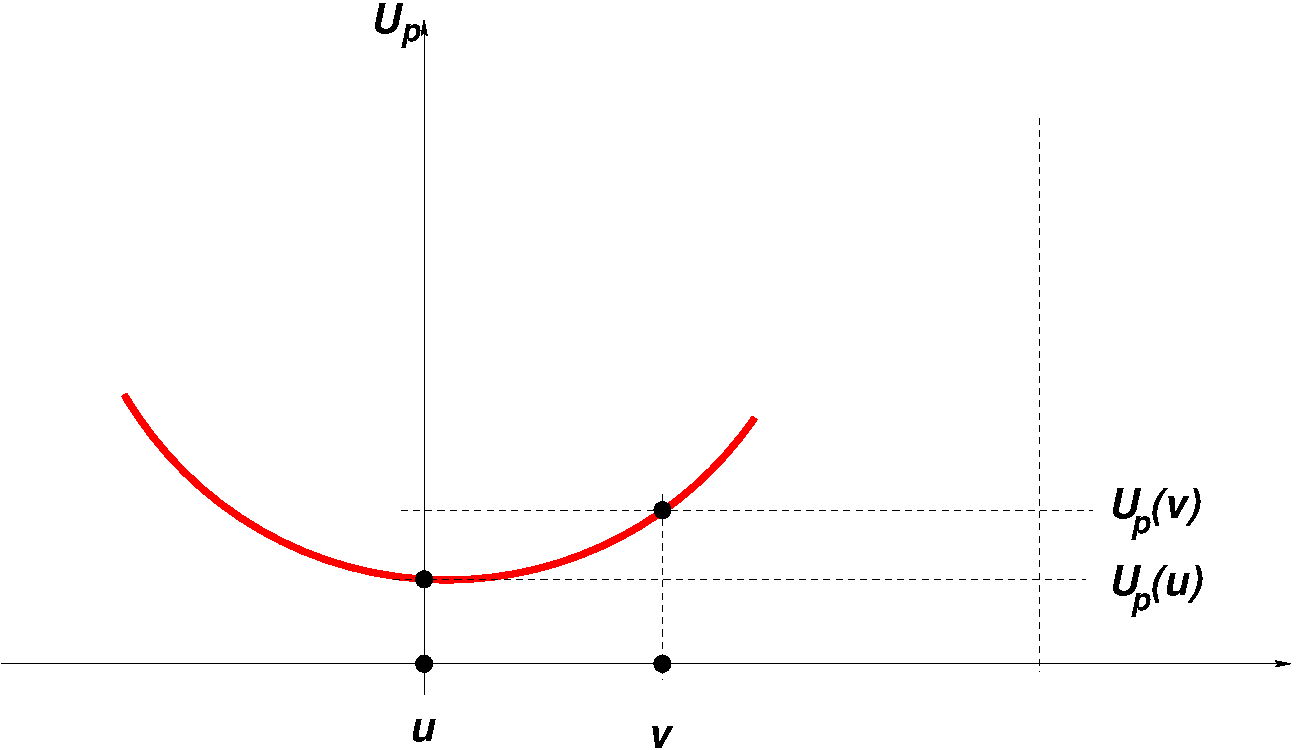
\includegraphics[width=0.9\textwidth]{figures/ch2/convex_minimum.pdf}
\end{minipage}\hfill
\begin{minipage}{0.45\textwidth}\centering
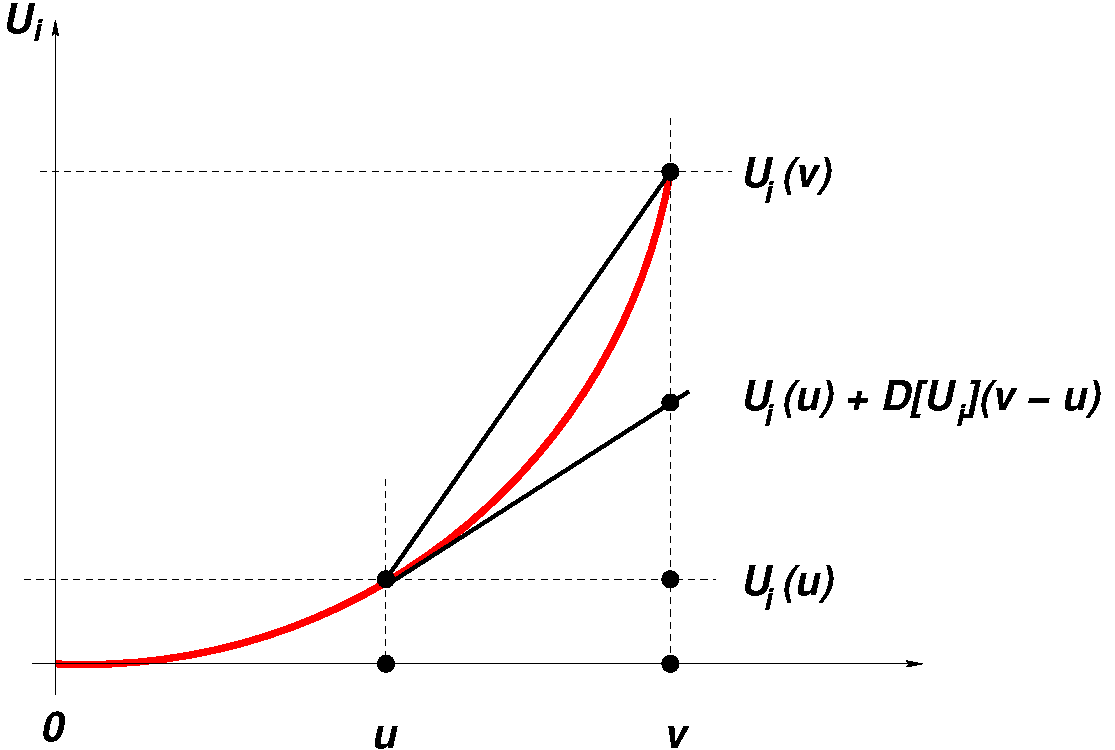
\includegraphics[width=0.9\textwidth]{figures/ch2/convex_du.pdf}
\end{minipage}
\caption{Left: the potential energy is minimal at $\vu$. Right: a convex
function lies above its tangent, $\mathcal U_i(\vv)\ge\mathcal U_i(\vu)+D\mathcal U_i(\vu)(\vv-\vu)$.}
\label{fig:convexity}
\end{figure}

\begin{figure}[h]
\centering
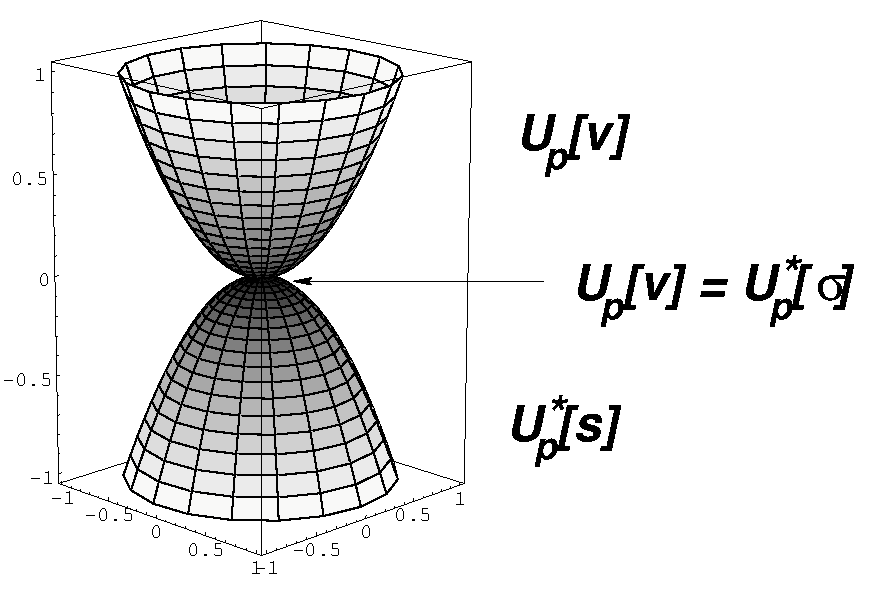
\includegraphics[height=6cm]{figures/ch2/energy_scheme.pdf}
\caption{The potential energy $\mathcal U_p[\vv]$ (a convex bowl over
kinematically admissible fields) and the complementary energy
$\mathcal U_p^\ast[\tens{s}]$ (a concave cap over statically admissible
fields) touch at the solution.}
\label{fig:energy-scheme}
\end{figure}

\subsection{The Lagrangian of the potential energy}\label{ssec:el-lagrangian}
\index{Lagrangian!potential energy}\index{Lagrange multiplier!reaction force}\index{thermoelasticity!Lagrangian}%
The minimum principle is posed on the constrained set $\Kad(\vuD,S_u)$.
Following~\cite{BonnetFrangi2007}, the constraint can be relaxed with a
Lagrange multiplier on $S_u$, which yields all the equations, including the
boundary conditions and the reactions, from a single stationarity condition.

\begin{gbox}{Lagrangian of thermoelasticity}
For unconstrained fields $\vv$ and multipliers $\vlambda$ on $S_u$,
\begin{multline}\label{eq:L-el}
  \mathcal L(\vv,\vlambda)=\int_\Omega\Bigl(\sig_0:\eps[\vv]
  +\tfrac12\bigl(\eps[\vv]-\talpha\theta^D\bigr):\bbC:\bigl(\eps[\vv]-\talpha\theta^D\bigr)\Bigr)\dd x\\
  -\int_\Omega\vfD\cdot\vv\dd x-\int_{S_t}\vtD\cdot\vv\dd s
  -\int_{S_u}\vlambda\cdot(\vv-\vuD)\dd s .
\end{multline}
The solution $(\vu,\vlambda)$ is a saddle point of $\mathcal L$: a minimum in
$\vv$ and a maximum in $\vlambda$.
\end{gbox}
\paragraph{Derivation of the equations.} Write
$\sig=\sig_0+\bbC:(\eps[\vu]-\talpha\theta^D)$. Stationarity with respect to
$\vlambda$ gives $\vu=\vuD$ on $S_u$. Stationarity with respect to $\vv$, in
every direction $\vw$, gives
\[
  \int_\Omega\sig:\eps[\vw]\dd x-\int_\Omega\vfD\cdot\vw\dd x
  -\int_{S_t}\vtD\cdot\vw\dd s-\int_{S_u}\vlambda\cdot\vw\dd s=0 .
\]
Integrating by parts with Theorem~\ref{thm:ibp-tensor},
\[
  \int_\Omega(-\dive\sig-\vfD)\cdot\vw\dd x+\int_{S_t}(\sig\vn-\vtD)\cdot\vw\dd s
  +\int_{S_u}(\sig\vn-\vlambda)\cdot\vw\dd s=0\qquad\forall\vw,
\]
hence the balance $\dive\sig+\vfD=\vzero$ in $\Omega$, the traction condition
$\sig\vn=\vtD$ on $S_t$, and $\vlambda=\sig\vn$ on $S_u$: the multiplier is
the traction exerted by the support, the reaction, with its sign. This is
the reason for the minus sign in front of the constraint
in~\eqref{eq:L-el}; the discrete system~\eqref{eq:saddle} keeps the same
convention. The constitutive law,
with its thermal and initial-stress terms, is contained in the definition of
the energy density.

The Lagrangian of diffusion, built in the same way, is given in
Section~\ref{ssec:diff-lagrangian}.

\paragraph{Remark: two-field Lagrangians.} Relaxing also the constitutive law,
with the stress as an independent field, gives the Hellinger--Reissner
functional, and relaxing the compatibility $\eps=\eps[\vu]$ the Hu--Washizu
functional~\cite{BonnetFrangi2007}. They are the basis of mixed finite
elements, used for incompressible materials.

%======================================================================
\section{Approximate solutions: from Ritz--Galerkin to finite elements}\label{sec:el-ritz}
\index{Ritz--Galerkin method}\index{approximate solution}%
Closed-form solutions exist only for simple geometries. The equations can be
solved approximately by finite differences, by series expansions, or by the
energy principle: the Ritz--Rayleigh/Galerkin technique, of which finite
elements are a particular case.

\subsection{The Ritz--Galerkin method}
\begin{gbox}{Ritz--Galerkin approximation}
The approximate solution $\vu^A$ minimizes the potential energy over a
finite-dimensional subset $\Kad_A\subset\Kad(\vuD,S_u)$ of admissible
displacement fields:
\[
  \vu^A=\argmin_{\vv\in\Kad_A}\mathcal U_p[\vv].
\]
\end{gbox}
\begin{figure}[h]
\centering
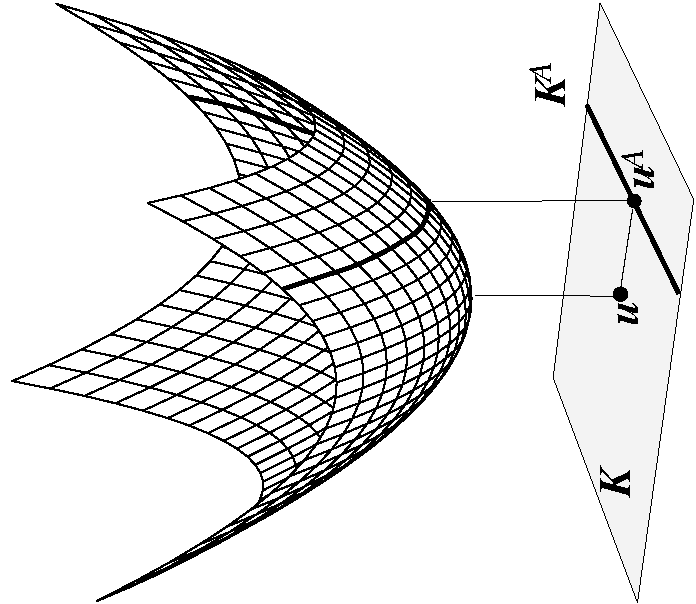
\includegraphics[angle=-90,width=0.38\textwidth]{figures/ch2/approximate_solution.pdf}
\caption{The Ritz approximation minimizes the same energy on a smaller set
$\Kad^A\subset\Kad$; by the minimum principle,
$\mathcal U_p(\vu)\le\mathcal U_p(\vu^A)$.}
\label{fig:ritz}
\end{figure}
Write the trial fields as combinations of $M$ given fields with unknown
coefficients:
\[
  \vv[\vect{\alpha}]=\sum_{m=1}^M\alpha_m\vw_m,\qquad
  \vect{\alpha}=(\alpha_1,\dots,\alpha_M)\in\R^M .
\]
For homogeneous data on $S_u$ (otherwise add a fixed field satisfying
$\vv=\vuD$), the energy is a quadratic function of $\vect{\alpha}$,
\[
  \mathcal U_p(\vv[\vect{\alpha}])=\tfrac12\vect{\alpha}\T\mat{K}\vect{\alpha}-\vect{\beta}\T\vect{\alpha},
\]
\[
  K_{m\ell}=\int_\Omega\eps[\vw_m]:\bbC:\eps[\vw_\ell]\dd x,\qquad
  \beta_m=\int_\Omega\vfD\cdot\vw_m+\int_{S_t}\vtD\cdot\vw_m .
\]
The stiffness matrix $\mat{K}$ is symmetric (major symmetry of $\bbC$) and
positive definite (positivity of $\bbC$, independent $\vw_m$ and no rigid
motion). By Theorem~\ref{thm:min-discrete} the minimum is the solution of
\[
  \mat{K}\vect{\alpha}=\vect{\beta},\qquad
  \vu^A=\sum_{m=1}^M\alpha_m\vw_m .
\]

\subsection{Imposed displacements as constraints}\label{ssec:ritz-lagrange}
\index{Lagrange multiplier!imposed displacements}\index{reaction forces}%
Instead of building the boundary conditions into the trial fields, write
them as linear constraints on the unknowns, $\mat{P}\vu=\vuD$, and minimize
the potential energy subject to them (Section~\ref{sec:var-lagrange}). As in
the continuous Lagrangian~\eqref{eq:L-el}, the constraint enters with a minus
sign. The solution is the saddle point of
\[
  \mathcal L(\vu,\vlambda)=\tfrac12\vu\T\mat{K}\vu-\mat{F}\T\vu-\vlambda\T(\mat{P}\vu-\vuD),
  \qquad
  \frac{\partial\mathcal L}{\partial\vu}=\vzero,\quad
  \frac{\partial\mathcal L}{\partial\vlambda}=\vzero,
\]
that is
\begin{equation}\label{eq:saddle}
  \begin{bmatrix}\mat{K}&-\mat{P}\T\\ -\mat{P}&\mat{0}\end{bmatrix}
  \begin{bmatrix}\vu\\ \vlambda\end{bmatrix}=
  \begin{bmatrix}\mat{F}\\ -\vuD\end{bmatrix}.
\end{equation}
The first line reads $\mat{K}\vu=\mat{F}+\vect{r}$ with $\vect{r}=\mat{P}\T\vlambda$:
the multipliers are the reaction forces at the constrained degrees of freedom,
with their sign (Exercise~\ref{exo:lagrange-el}). The matrix is symmetric but
indefinite. $\mat{K}$ alone may be singular, since the supports are now in
$\mat{P}$. If $\mat{K}$ is positive definite on the kernel of $\mat{P}$ and
the constraints are independent, the solution is unique. Cast3M, for instance, imposes
displacement conditions this way.

\subsection{Which trial functions?}
\index{conditioning}\index{trial functions}%
\begin{itemize}
\item \emph{Global bases} of $L^2(\Omega)$. Polynomials give a full,
badly conditioned matrix $\mat{K}$: its eigenvalues spread over many orders of
magnitude as the degree grows, and the numerical inversion becomes unstable
(Exercise~\ref{exo:conditioning}). Trigonometric functions are suited only to
particular domains, and $\mat{K}$ is still full.
\item \emph{Finite elements}: piecewise polynomials on a partition of the
domain, continuous across the subdomains. The matrix is sparse and well
conditioned.
\item \emph{Isogeometric analysis}~\cite{HughesCottrellBazilevs2005,CottrellHughesBazilevs2009}:
\index{isogeometric analysis}\index{NURBS}%
the trial functions are the B-splines or NURBS that describe the exact CAD
geometry, smoother than standard elements ($C^{p-1}$ for degree $p$). They
are presented and compared with finite elements in
Section~\ref{sec:var-iga}.
\end{itemize}

\subsection{Finite elements}
\index{finite element method}\index{mesh}%
The finite element method is the Ritz--Galerkin method with a particular
choice of $\vw_m$: the domain $\Omega$ is approximated by a mesh $\Omega_h$
of elements, $\Omega_h\to\Omega$ as $h\to0$, and the unknowns are the nodal
values of the displacement,
\[
  \vu_h(\vx)=\sum_{m}u_i(\vx_m)\,w_m(\vx)\,\ve_i ,
\]
where $w_m$ is the shape function of node $m$: equal to $1$ at node $m$, $0$ at
the other nodes, polynomial on each element (Figure~\ref{fig:fem}).
\begin{figure}[h]
\centering
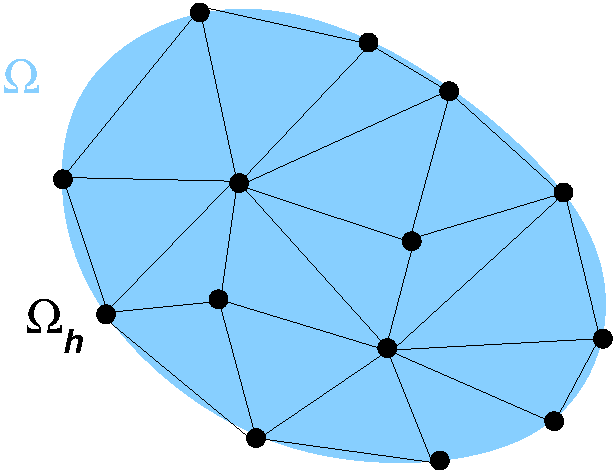
\includegraphics[width=0.3\textwidth]{figures/ch2/fem_mesh.pdf}\qquad\qquad
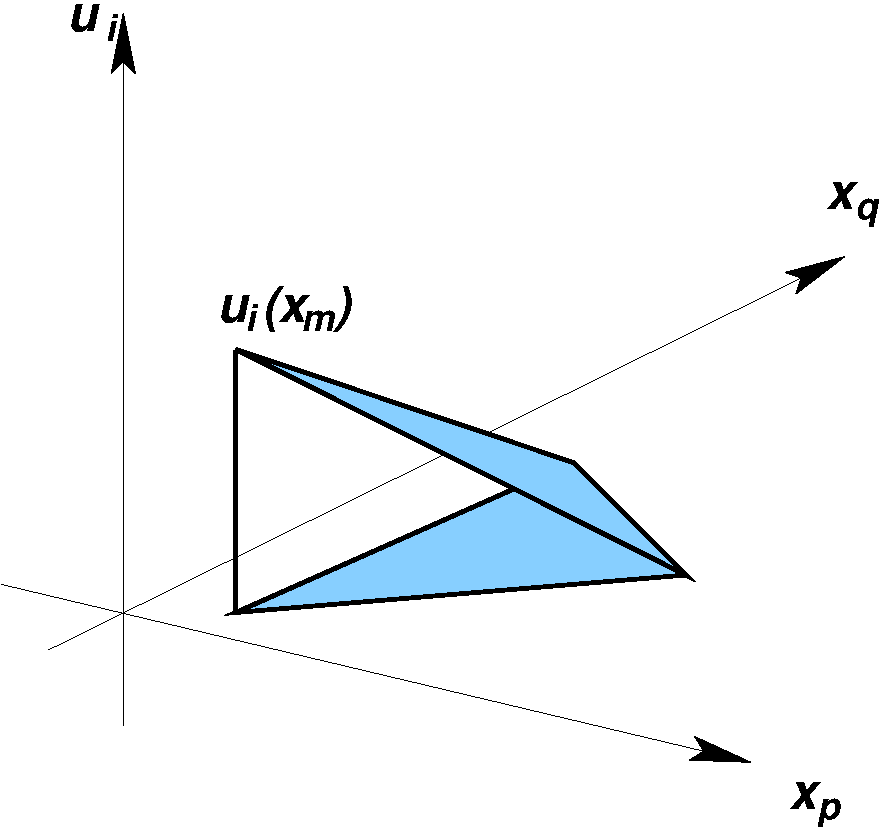
\includegraphics[width=0.36\textwidth]{figures/ch2/fem_element.pdf}
\caption{Left: a mesh $\Omega_h$ of the domain $\Omega$. Right: the shape
function of a node, linear on each triangle.}
\label{fig:fem}
\end{figure}

\paragraph{Shape functions.}
\index{finite element method!shape functions}\index{Hermite cubics}%
\begin{itemize}
\item \emph{Linear elements in one dimension:} $w=a+bx$; the unknowns are the
nodal values.
\item \emph{Cubic elements in one dimension} (Hermite cubics):
$w=a+bx+cx^2+dx^3$; the unknowns are the nodal values and slopes (beams).
Splines are not defined by nodal values alone and do not qualify as finite
elements in the sense of Ciarlet (Section~\ref{sec:var-bsplines}).
\item \emph{Bilinear elements on rectangles:} $w=a+bx+cy+dxy$.
\item \emph{Triangles:} linear, $w=a+bx+cy$, with nodes at the vertices;
quadratic, $w=a+bx+cy+dx^2+exy+fy^2$, with nodes at the vertices and the
mid-edges (Figure~\ref{fig:shape}).
\end{itemize}
\begin{figure}[h]
\centering
\begin{tabular}{ccc}
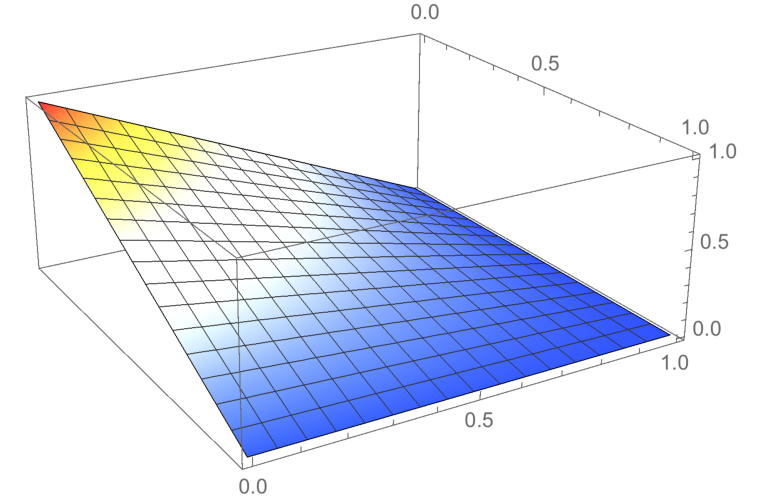
\includegraphics[height=2.4cm]{figures/ch2/P1_rectangle.pdf} &
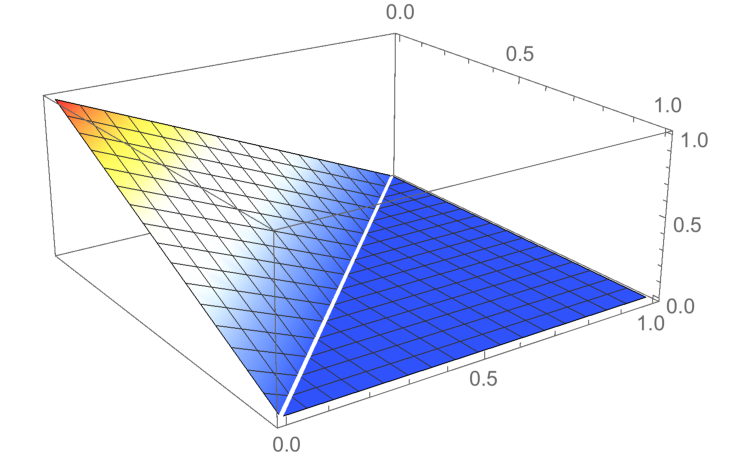
\includegraphics[height=2.4cm]{figures/ch2/P1_triangle.pdf} &
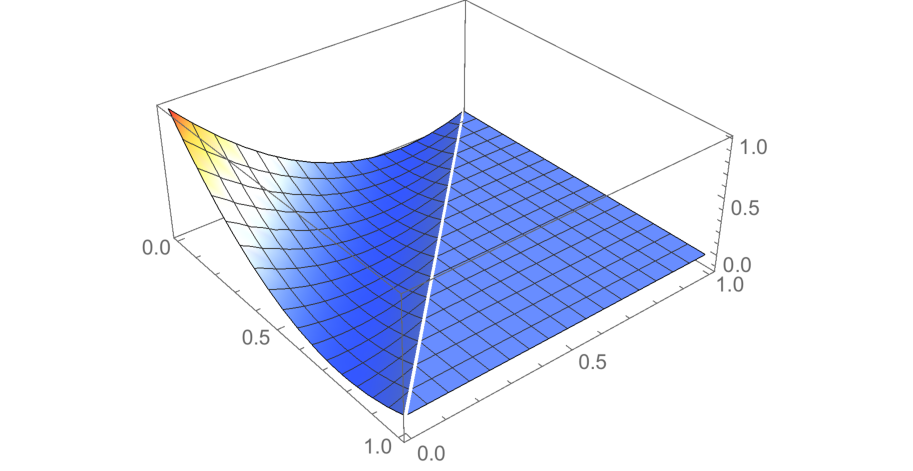
\includegraphics[height=2.4cm]{figures/ch2/P2_triangle.pdf}\\
{\small bilinear, rectangle} & {\small linear, $w=1-x-y$} & {\small quadratic, $w=(1-x-y)(1-2x-2y)$}
\end{tabular}
\caption{Shape functions of the node at the origin for three elements.}
\label{fig:shape}
\end{figure}

\paragraph{Numerical integration with Gauss points.}
\index{finite element method!Gauss points}\index{Gauss quadrature}%
The stiffness matrix is the sum of element contributions,
$\mat{K}=\sum_e\mat{K}_e$, each assembled at the rows and columns of the nodes
of element $e$. Each element is the image of a reference element
$\hat\Omega$ (the segment $[-1,1]$, the square $[-1,1]^2$, the unit triangle) by
a map $\vx(\vxi)$ with Jacobian matrix $\mat{J}=\partial\vx/\partial\vxi$
(Figure~\ref{fig:refmap}). In the \emph{isoparametric} map the geometry is
\index{isoparametric element}\index{Jacobian of the element map}%
interpolated like the displacement, $\vx(\vxi)=\sum_aN_a(\vxi)\,\vx_a$, with
the shape functions $N_a$ of the reference element and the nodes $\vx_a$. The
columns of $\mat{J}$ are the tangent vectors to the coordinate lines, and the
volume element is $\dd x=\det\mat{J}\dd\xi$. The map must be one-to-one,
$\det\mat{J}>0$ in the element: a badly distorted quadrilateral is rejected by
the code. The integral is computed on the reference element by a quadrature
rule:
\[
  \mat{K}_e=\int_{\Omega_e}\mat{B}\T\mat{C}\mat{B}\dd x
  =\int_{\hat\Omega}\mat{B}\T\mat{C}\mat{B}\,\det\mat{J}\dd\xi
  \approx\sum_{g=1}^{n_g}w_g\,\mat{B}\T(\vxi_g)\,\mat{C}\,\mat{B}(\vxi_g)\,\det\mat{J}(\vxi_g).
\]
The points $\vxi_g$ and weights $w_g$ of Gauss--Legendre quadrature are chosen
so that $n$ points integrate exactly the polynomials of degree $2n-1$ on
$[-1,1]$: one point $\xi=0$, $w=2$ (degree 1); two points
$\xi=\pm1/\sqrt3$, $w=1$ (degree 3); three points $0,\pm\sqrt{3/5}$ with
weights $\tfrac89,\tfrac59$ (degree 5). On quadrilaterals the rule is the
tensor product, $2\times2$ points for bilinear elements. On triangles, one
point at the centroid integrates linear functions, and the three points of
Figure~\ref{fig:gauss}, $(\tfrac16,\tfrac16)$, $(\tfrac23,\tfrac16)$,
$(\tfrac16,\tfrac23)$ with weights $\tfrac16$, integrate quadratics. The rule is
chosen to integrate the stiffness exactly for affine elements; fewer points
(reduced integration) soften the element, and too few produce spurious
zero-energy modes. The Gauss points are where the strains and stresses are
computed; for nonlinear materials they are also where the internal variables
(plastic strain, damage) are stored and the constitutive law is integrated,
which is the subject of the next part of the course.
\begin{figure}[h]
\centering
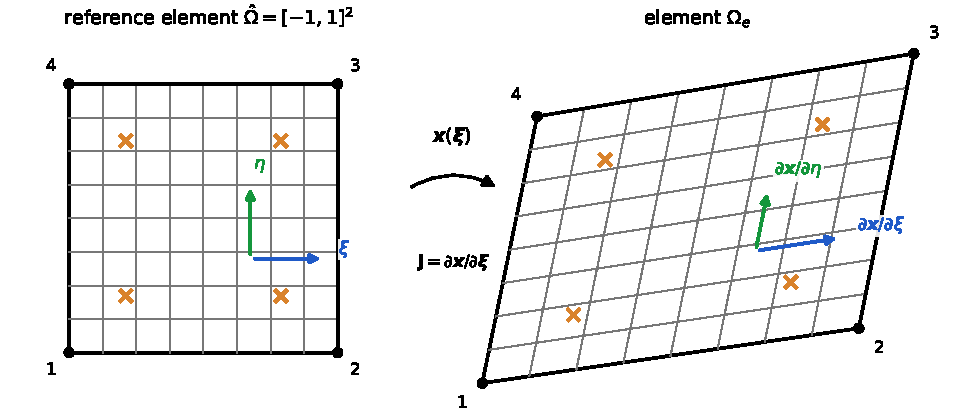
\includegraphics[width=0.85\textwidth]{figures/ch2/reference_map.pdf}
\caption{The isoparametric map $\vx(\vxi)=\sum_aN_a(\vxi)\,\vx_a$ of a
bilinear quadrilateral. The coordinate lines of the reference square are
mapped to straight lines of the element, no longer parallel; the columns of
$\mat{J}=\partial\vx/\partial\vxi$ are their tangent vectors. Crosses: the
$2\times2$ Gauss points and their images.}
\label{fig:refmap}
\end{figure}

\paragraph{Matrix structure.} The discrete equations reproduce the Tonti
\index{Tonti diagram!finite elements}\index{finite element method!Gauss points}%
diagram (Figure~\ref{fig:tonti-fem}):
\[
  \bigl(\mat{B}\T\mat{C}\mat{B}\bigr)\,\mat{u}=\mat{F},\qquad \mat{P}\mat{u}=\mat{u}^D,
\]
where $\mat{u}$ collects the nodal displacements, $\mat{B}$ computes the
strains from them, $\mat{C}$ is the matrix of $\bbC$ and $\mat{F}$ collects the
nodal forces equivalent to $\vfD$ and $\vtD$. Strains and stresses are
computed at the Gauss points of each element, where the integrals are
evaluated numerically (Figure~\ref{fig:gauss}).
\begin{figure}[h]
\centering
\begin{tikzpicture}[node distance=1.0cm and 1.1cm]
  \node[tinybox,kin,text width=3.2cm,minimum width=3.5cm] (u) {$\mat{u}$, \ $\mat{P}\mat{u}=\mat{u}^D$\\ \scriptsize nodal displacements};
  \node[tinybox,stat,text width=3.2cm,minimum width=3.5cm,right=4.2cm of u] (f) {$\mat{F}$\\ \scriptsize nodal forces};
  \node[tinybox,kin,text width=3.2cm,minimum width=3.5cm,below=of u] (e) {$\mat{e}=\mat{B}\mat{u}$\\ \scriptsize strains at Gauss points};
  \node[tinybox,stat,text width=3.2cm,minimum width=3.5cm,below=of f] (s) {$\mat{s}=\mat{C}\mat{e}$\\ \scriptsize stresses at Gauss points};
  \draw[arr] (u) -- (e) node[midway,left,font=\small]{$\mat{B}$};
  \draw[arr] (e) -- (s) node[midway,below,font=\small]{$\mat{C}$};
  \draw[arr] (s) -- (f) node[midway,right,font=\small]{$\mat{B}\T$};
  \node[below=0.15cm of e,kinlab] {kinematic};
  \node[below=0.15cm of s,statlab] {static};
\end{tikzpicture}
\caption{The discrete Tonti diagram of the finite element method; compare
with Figures~\ref{fig:tonti-discrete} and~\ref{fig:tonti-el}.}
\label{fig:tonti-fem}
\end{figure}
\begin{figure}[h]
\centering
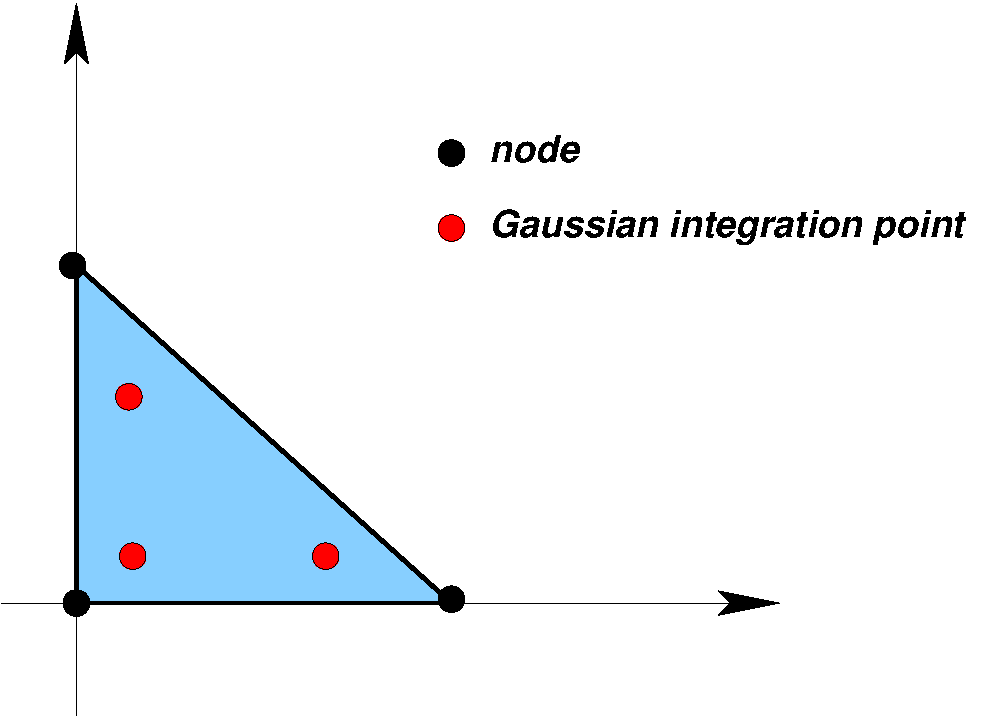
\includegraphics[width=0.45\textwidth]{figures/ch2/fem_point_gauss.pdf}
\caption{Nodes, where the displacements live, and Gauss points, where strains
and stresses are computed: $[\vu]\to\mat{B}\to[\eps]$ and
$[\sig]\to\mat{B}\T\to[\vf]$.}
\label{fig:gauss}
\end{figure}

\paragraph{A test case: the plate with a hole.} A finite element code is
\index{Kirsch problem}\index{stress concentration}%
checked against closed-form solutions. The classical one is the infinite
plate with a circular hole under a remote tension $\sigma$, solved by
Kirsch~\cite{Kirsch1898}: the hoop stress on the hole reaches $3\sigma$, a
stress concentration factor of $3$ whatever the radius. A small program with
linear triangles recovers it within $1\%$ with a few thousand unknowns,
provided the mesh is refined near the hole (Exercise~\ref{exo:kirsch},
Figure~\ref{fig:kirsch}).

%======================================================================
\framepart{Summary}
\begin{gbox*}
\begin{itemize}
  \item \textbf{The same structure} appears in all frameworks: discrete
  springs, diffusion, elasticity, finite elements (Table~\ref{tab:diff-el},
  Figures~\ref{fig:tonti-diff}, \ref{fig:tonti-el} and~\ref{fig:tonti-fem}):
  kinematic quantities and data (blue), static quantities and data (green),
  joined by the material law $\tk$ or $\bbC$.
  \item \textbf{Adjoint and transpose.} The adjoint of $\nabla$ and of
  $\eps[\cdot]$ is the pair formed by $-\dive$ in $\Omega$ and the boundary
  trace $\cdot\,\vn$ on $S_\varphi$ or $S_t$, the flux or the traction on the
  boundary. It corresponds to the transpose matrix $\mat{B}\T$; virtual work
  expresses this duality.
  \item \textbf{The Lagrangian} of the potential energy, with a multiplier
  for the imposed displacements or potentials, yields all the equations at
  once; the multiplier is the reaction (traction or flux) on $S_u$.
  \item \textbf{Elastic moduli.} $\bbC$ has minor and major symmetries
  ($21$ moduli in general, $2$ for isotropy) and must be positive definite:
  $K>0$, $\mu>0$, i.e.\ $E>0$ and $-1<\nu<\tfrac12$.
  \item \textbf{Uniqueness} follows from convexity, i.e.\ the positive
  definiteness of the energy, and from the displacement boundary conditions,
  which eliminate rigid motions.
  \item \textbf{Two energy principles} bound the solution from both sides;
  the Ritz--Galerkin and finite element methods minimize the potential energy
  on a finite-dimensional space, and imposed displacements can be enforced by
  Lagrange multipliers, the reactions.
\end{itemize}
\end{gbox*}

%======================================================================
\framepart{Exercises}\label{sec:el-exo}

\framesub{Short questions}
No documents, no computer: each question needs a few lines of computation.

\exercise{Boundary conditions}\label{exo:q-bc}
\index{boundary condition!elasticity}%
A cube $[0,a]^3$ rests on a frictionless rigid table, the plane $x_3=0$. A
uniform pressure $p$ acts on its top face; the lateral faces are free. Write
the boundary conditions on each face. Is the solution unique?
\begin{solution}
Bottom face: $u_3=0$ and $\sigma_{13}=\sigma_{23}=0$ (frictionless contact). Top
face: $\sig\vn=-p\,\ve_3$, i.e.\ $\sigma_{33}=-p$, $\sigma_{13}=\sigma_{23}=0$.
Lateral faces: $\sig\vn=\vzero$. The stress is unique,
$\sig=-p\,\ve_3\otimes\ve_3$. The displacement is unique up to the rigid
motions allowed by $u_3=0$: the translations along $\ve_1$, $\ve_2$ and the
rotation about $\ve_3$. Fixing three components at two points of the bottom
face removes them.
\end{solution}

\exercise{Engineering constants}\label{exo:q-constants}
A steel has $E=200$\,GPa and $\nu=0.25$. (a) Compute $\lambda$, $\mu$ and $K$.
(b) A bar carries a uniaxial stress $\sigma=100$\,MPa. Compute
$\varepsilon_{11}$, $\varepsilon_{22}$ and the relative change of volume.
\begin{solution}
(a) $\lambda=\nu E/\bigl((1+\nu)(1-2\nu)\bigr)=80$\,GPa,
$\mu=E/\bigl(2(1+\nu)\bigr)=80$\,GPa, $K=E/\bigl(3(1-2\nu)\bigr)=133$\,GPa.
(b) $\varepsilon_{11}=\sigma/E=5\times10^{-4}$,
$\varepsilon_{22}=\varepsilon_{33}=-\nu\sigma/E=-1.25\times10^{-4}$, and
$\tr\eps=(1-2\nu)\sigma/E=\sigma/(3K)=2.5\times10^{-4}$.
\end{solution}

\exercise{Is this material stable?}\label{exo:q-stable}
\index{auxetic material}%
A polymer foam is measured with $E=1$\,MPa and $K=0.2$\,MPa. Compute $\nu$
and $\mu$. Is the elastic energy positive definite?
\begin{solution}
$K=E/\bigl(3(1-2\nu)\bigr)$ gives $1-2\nu=E/(3K)=\tfrac53$, so $\nu=-\tfrac13$.
Then $\mu=E/\bigl(2(1+\nu)\bigr)=0.75$\,MPa. Since $K>0$ and $\mu>0$, the energy
is positive definite~\eqref{eq:iso-energy}: the foam is stable, and auxetic.
\end{solution}

\exercise{Why Korn?}\label{exo:q-korn}
\index{Korn's inequality}%
Take $\vv=\omega\,\ve_3\times\vx$ on the unit cube. Compute $\eps[\vv]$ and
$\nabla\vv$. Why is the positive definiteness of $\bbC$ not enough to make the
elastic form coercive on $H^1(\Omega)^3$? What changes when $|S_u|>0$?
\begin{solution}
$\vv=\omega(-x_2,x_1,0)$, so $\nabla\vv=\omega(\ve_2\otimes\ve_1-\ve_1\otimes\ve_2)$
is skew and $\eps[\vv]=\vzero$. The energy vanishes while
$\norm{\vv}_{H^1}>0$: no inequality $a(\vv,\vv)\ge c\norm{\vv}^2_{H^1}$ can hold
on $H^1(\Omega)^3$. If $\vv=\vzero$ on a part $S_u$ of positive area, the only
rigid motion allowed is zero, and Korn's inequality restores coercivity.
\end{solution}

\exercise{Is this crystal isotropic?}\label{exo:q-zener}
\index{Zener ratio}%
With Table~\ref{tab:el-stiffness}, compute the Zener ratio
$A=2c_{44}/(c_{11}-c_{12})$ of aluminium and of tungsten. For tungsten,
deduce $E$ and $\nu$ from $s_{11}=0.257$ and $s_{12}=-0.073$, in
$10^{-11}\,\mathrm{Pa}^{-1}$.
\begin{solution}
Aluminium: $A=56/46=1.22$, mildly anisotropic. Tungsten: $A=304/303=1.00$,
isotropic. Then $E=1/s_{11}=389$\,GPa and $\nu=-s_{12}/s_{11}=0.28$. Check:
$\mu=E/\bigl(2(1+\nu)\bigr)=152$\,GPa$\,=c_{44}$.
\end{solution}

\exercise{Weak form of a bar}\label{exo:q-weak}
\index{weak form!diffusion}%
Write the weak form of $-(ku')'=f$ on $(0,L)$, with $u(0)=u_0$ and
$k\,u'(L)=\varphi$. Which condition is essential, which is natural? Which
energy does $u$ minimize?
\begin{solution}
Multiply by $v$ with $v(0)=0$ and integrate by parts:
$\displaystyle \int_0^Lku'v'\dd x=\int_0^Lfv\dd x+\varphi\,v(L)$ for all such $v$, with
$u(0)=u_0$. The condition $u(0)=u_0$ is essential (it defines the space); the
flux $\varphi$ is natural (it enters the right-hand side). The solution
minimizes
$\displaystyle J(v)=\int_0^L\tfrac12k(v')^2\dd x-\int_0^Lfv\dd x-\varphi\,v(L)$ over
$v(0)=u_0$.
\end{solution}

\exercise{One spring, one multiplier}\label{exo:q-saddle}
\index{Lagrange multiplier!reaction force}%
A spring of stiffness $k$ joins a fixed point to a node loaded by a force $F$.
The displacement of the node is imposed, $u=\uD$, by a Lagrange multiplier as
in~\eqref{eq:saddle}. Write the $2\times2$ system, solve it and interpret
$\lambda$.
\begin{solution}
\[
\begin{bmatrix}k&-1\\-1&0\end{bmatrix}\begin{bmatrix}u\\ \lambda\end{bmatrix}
=\begin{bmatrix}F\\ -\uD\end{bmatrix}.
\]
The second line gives $u=\uD$, the first
$\lambda=k\uD-F$. The multiplier is the reaction $r=\lambda$: the support adds
the force $k\uD-F$ to $F$ to balance the spring force $k\uD$. If $F=k\uD$ no
reaction is needed.
\end{solution}

\exercise{A hole under biaxial loads}\label{exo:q-hole}
\index{stress concentration}%
Under a remote tension $\sigma$ along $\ve_1$, the hoop stress on a circular
hole in an infinite plate is $\sigma_{\theta\theta}=\sigma(1-2\cos2\theta)$
(Exercise~\ref{exo:kirsch}). By superposition, find $\sigma_{\theta\theta}$ on
the hole under (a) an equibiaxial tension $\sigma$ along $\ve_1$ and $\ve_2$;
(b) a pure shear, $\sigma$ along $\ve_1$ and $-\sigma$ along $\ve_2$. Give the
stress concentration factor in each case.
\begin{solution}
A tension along $\ve_2$ is the tension along $\ve_1$ rotated by $\tfrac\pi2$:
$\theta\to\theta-\tfrac\pi2$ changes $\cos2\theta$ into $-\cos2\theta$, so
it gives $\sigma(1+2\cos2\theta)$. (a) The sum is $2\sigma$, uniform on the
hole: factor $2$. (b) The difference is $-4\sigma\cos2\theta$: factor $4$. A
hole is most harmful in shear.
\end{solution}

\exercise{Zero-energy modes}\label{exo:q-modes}
\index{hourglass mode}%
A four-node quadrilateral in plane elasticity has $8$ degrees of freedom.
With one Gauss point, what is the largest possible rank of its stiffness
matrix? How many zero-energy modes does it have, and how many are spurious?
Same questions with $2\times2$ Gauss points.
\begin{solution}
With one point, $\mat{K}_e=w\,\mat{B}\T\mat{C}\mat{B}\det\mat{J}$ with $\mat{B}$ of
size $3\times8$: the rank is at most $3$. At least $8-3=5$ modes have zero
energy: $3$ rigid motions and $2$ spurious hourglass modes
(Exercise~\ref{exo:gauss}). With $2\times2$ points the rank is $8-3=5$: only
the rigid motions remain.
\end{solution}

\framesub{Elastic moduli and energy principles}

\exercise{Lam\'e and engineering constants}\label{exo:lame}
(a) From $\sig=\lambda(\tr\eps)\tI+2\mu\eps$, compute the response to a
uniaxial stress $\sig=\sigma\,\ve_1\otimes\ve_1$ and derive $E$ and $\nu$ in
terms of $\lambda,\mu$. (b) Derive the bulk modulus $K$ from a hydrostatic
stress $\sig=-p\tI$. (c) Invert the law and check the expression of $\bbS$.
\begin{solution}
(a) Taking the trace, $\tr\sig=(3\lambda+2\mu)\tr\eps$, so
$\displaystyle \eps=\frac{1}{2\mu}\bigl(\sig-\frac{\lambda}{3\lambda+2\mu}(\tr\sig)\tI\bigr)$.
For uniaxial stress, $\displaystyle \varepsilon_{11}=\frac{\lambda+\mu}{\mu(3\lambda+2\mu)}\sigma$
and $\displaystyle \varepsilon_{22}=-\frac{\lambda}{2\mu(3\lambda+2\mu)}\sigma$, so
$E=\sigma/\varepsilon_{11}=\mu(3\lambda+2\mu)/(\lambda+\mu)$ and
$\nu=-\varepsilon_{22}/\varepsilon_{11}=\lambda/(2(\lambda+\mu))$.
(b) $\tr\eps=-3p/(3\lambda+2\mu)$, so $K=-p/\tr\eps=\lambda+\tfrac23\mu$.
(c) Substituting $\displaystyle \frac1{2\mu}=\frac{1+\nu}{E}$ and
$\displaystyle \frac{\lambda}{2\mu(3\lambda+2\mu)}=\frac{\nu}{E}$ in (a) gives
$\displaystyle \eps=\frac{1+\nu}{E}\sig-\frac{\nu}{E}(\tr\sig)\tI$, i.e.\ the expression of
$\bbS$ in the box.
\end{solution}

\exercise{Positive definiteness of isotropic elasticity}\label{exo:posdef}
\index{incompressibility}%
(a) Prove~\eqref{eq:iso-energy}. (b) Show that $\bbC$ is positive definite iff
$K>0$ and $\mu>0$. (c) Show that this is equivalent to $E>0$ and
$-1<\nu<\tfrac12$. What happens as $\nu\to\tfrac12$?
\begin{solution}
(a) With $\eps=\tfrac13(\tr\eps)\tI+\dev\eps$ and $\tr\dev\eps=0$:
$\eps:\eps=\tfrac13(\tr\eps)^2+\dev\eps:\dev\eps$, so
$\lambda(\tr\eps)^2+2\mu\,\eps:\eps=(\lambda+\tfrac23\mu)(\tr\eps)^2+2\mu\,\dev\eps:\dev\eps$.
(b) The two terms are independent (a pure dilatation has $\dev\eps=\vzero$,
a pure shear has $\tr\eps=0$), so positivity for all $\eps\ne\vzero$ holds iff
$K>0$ and $\mu>0$.
(c) $\mu=E/(2(1+\nu))$ and $K=E/(3(1-2\nu))$. Both positive with $E>0$ iff
$1+\nu>0$ and $1-2\nu>0$; $E<0$ would make both denominators negative, which is
impossible. As $\nu\to\tfrac12$, $K\to\infty$: the material becomes
incompressible, and $\tr\eps=0$ becomes a constraint, handled with a Lagrange
multiplier, the pressure.
\end{solution}

\exercise{From compliances to stiffnesses}\label{exo:stiffness}
\index{elastic moduli!matrix representation}\index{compliance tensor}%
(a) A hexagonal crystal is transversely isotropic about $\ve_3$. Show that
$s_{66}=2(s_{11}-s_{12})$ and $c_{66}=\tfrac12(c_{11}-c_{12})$. (b) Build the
$6\times6$ Voigt compliance matrices of the crystals of
Table~\ref{tab:el-stiffness} from Nye's compliances: cubic ($s_{11}$,
$s_{12}$, $s_{44}$); tetragonal $4/mmm$ ($s_{66}$ independent); hexagonal;
trigonal ($s_{14}$, $s_{24}=-s_{14}$, $s_{56}=2s_{14}$,
$s_{66}=2(s_{11}-s_{12})$). Invert them and check their positive
definiteness. (c) Invert the measured stiffnesses of cadmium,
$c_{11}=114.5$, $c_{33}=50.85$, $c_{44}=19.85$, $c_{13}=39.9$,
$c_{66}=37.5$\,GPa, and compare with Nye's compliances $s_{33}=3.55$ and
$s_{13}=-0.93$, in $10^{-11}\,\mathrm{Pa}^{-1}$.
\begin{solution}
(a) Take the in-plane pure shear $\sigma_{11}=-\sigma_{22}=\tau$. It gives
$\varepsilon_{11}-\varepsilon_{22}=2(s_{11}-s_{12})\tau$. In axes rotated by
$45^\circ$ about $\ve_3$ the same state is a shear stress $\tau$ with
engineering strain $\gamma=\varepsilon_{11}-\varepsilon_{22}$. Isotropy in the
plane requires $\gamma=s_{66}\tau$ in every axes, hence
$s_{66}=2(s_{11}-s_{12})$. With $\tau=c_{66}\gamma$ and
$\tau=\tfrac12(c_{11}-c_{12})(\varepsilon_{11}-\varepsilon_{22})$ the same
argument gives $c_{66}=\tfrac12(c_{11}-c_{12})$.
(b) The stiffnesses are those of Table~\ref{tab:el-stiffness}; all matrices
are positive definite. The trigonal stiffness matrix has $c_{56}=c_{14}$: the
factor $2$ of $s_{56}$ comes from the engineering shear strains. Two-digit
compliances give stiffnesses accurate to a few percent only (copper:
$c_{11}=176$ instead of $168$\,GPa).
(c) $c_{12}=c_{11}-2c_{66}=39.5$\,GPa. The inverse gives $s_{11}=1.21$,
$s_{12}=-0.12$, $s_{13}=-0.86$, $s_{33}=3.31$, $s_{44}=5.04$ in
$10^{-11}\,\mathrm{Pa}^{-1}$. The sign of $s_{13}$ agrees with Nye: a tension
along the hexagonal axis contracts the basal plane. The magnitudes agree
within $8\%$, the scatter between two sets of measurements.
\lstinputlisting[firstline=4]{python/examples/ch2/elastic_constants.py}
\end{solution}

\exercise{The Navier equations as Euler--Lagrange equations}\label{exo:navier}
Derive the strong form of the minimum of $\mathcal U_p$~\eqref{eq:Up} (with
$\sig_0=\vzero$, $\theta^D=0$), including the natural boundary condition, and
write it for isotropic elasticity.
\begin{solution}
$\displaystyle D\mathcal U_p(\vu)[\vv]=\int_\Omega\eps[\vu]:\bbC:\eps[\vv]-\int_\Omega\vfD\cdot\vv-\int_{S_t}\vtD\cdot\vv=0$
for all $\vv$ vanishing on $S_u$. With $\sig=\bbC:\eps[\vu]$ symmetric and
Theorem~\ref{thm:ibp-tensor},
$\displaystyle \int_\Omega(\dive\sig+\vfD)\cdot\vv+\int_{S_t}(\vtD-\sig\vn)\cdot\vv=0$, so
$\dive\sig+\vfD=\vzero$ in $\Omega$ and $\sig\vn=\vtD$ on $S_t$ (natural). For
isotropy, $\dive\bigl(\lambda(\dive\vu)\tI+\mu(\nabla\vu+\nabla\vu\T)\bigr)
=\lambda\nabla\dive\vu+\mu\Delta\vu+\mu\nabla\dive\vu$, giving
$(\lambda+\mu)\nabla(\dive\vu)+\mu\Delta\vu+\vfD=\vzero$.
\end{solution}

\exercise{Equality of the potentials}\label{exo:equality}
With $\sig_0=\vzero$ and $\theta^D=0$, show that
$\displaystyle \mathcal U_p(\vu)=\mathcal U_p^\ast(\sig)=-\tfrac12\int_\Omega\sig:\eps[\vu]+\int_{S_u}\vuD\cdot\sig\vn$.
\begin{solution}
Virtual work with $\vv=\vu$ gives
$\displaystyle \int_\Omega\sig:\eps=\int_\Omega\vfD\cdot\vu+\int_{S_t}\vtD\cdot\vu+\int_{S_u}(\sig\vn)\cdot\vuD$.
Hence
$\displaystyle \mathcal U_p(\vu)=\tfrac12\int\sig:\eps-\int\vfD\cdot\vu-\int_{S_t}\vtD\cdot\vu=-\tfrac12\int\sig:\eps+\int_{S_u}\vuD\cdot\sig\vn$.
On the other hand $\sig:\bbS:\sig=\sig:\eps$, so $\mathcal U_p^\ast(\sig)$ has
the same value. Without imposed displacements ($\vuD=\vzero$) the common
value is $\displaystyle -\tfrac12\int\sig:\eps$, minus the stored energy, as for the springs
($W_{\min}=-\tfrac12\vf\T\mat{K}^{-1}\vf$).
\end{solution}

\exercise{Complementary energy in diffusion}\label{exo:diff-comp}
\index{constitutive relation error}\index{a posteriori error estimation}%
With $\vp_0=\vzero$ and $\vect{g}^D=\vzero$, show that $J^\ast(\vq)\le J(v)$ for
all $v\in\Kad(\uD,S_u)$ and $\vq\in\Sad(f,\pD,S_\varphi)$
in~\eqref{eq:diffusion-energy}--\eqref{eq:diffusion-comp}, with equality at
the solution.
\begin{solution}
For $v$ and $\vq$ admissible, integrate by parts:
$\displaystyle \int_\Omega\vq\cdot\nabla v=-\int_\Omega(\dive\vq)v+\int_{\partial\Omega}(\vq\cdot\vn)v
=\int_\Omega fv+\int_{S_\varphi}\pD v+\int_{S_u}\uD\,\vq\cdot\vn$. Then
\[
  J(v)-J^\ast(\vq)=\frac12\int_\Omega(\tk\nabla v-\vq)\cdot\tk^{-1}(\tk\nabla v-\vq)\dd x\ge0 ,
\]
with equality iff $\vq=\tk\nabla v$, i.e.\ at the solution. The gap
$J(v)-J^\ast(\vq)$ is computable and bounds the error in energy norm: this is
the basis of a posteriori error estimation by constitutive relation error.
\end{solution}

\exercise{Anti-plane shear}\label{exo:antiplane}
\index{anti-plane shear}%
Let $\vu=w(x_1,x_2)\,\ve_3$ in an isotropic body. (a) Compute $\eps$ and
$\sig$. (b) Show that, without body forces, equilibrium reduces to $\Delta w=0$.
(c) What is the boundary condition on a traction-free crack face with normal
$\vn$ in the $(x_1,x_2)$ plane?
\begin{solution}
(a) $\varepsilon_{3\alpha}=\tfrac12w_{,\alpha}$, all other components zero;
$\tr\eps=0$, so $\sig=2\mu\eps$: $\sigma_{3\alpha}=\mu w_{,\alpha}$.
(b) $\sigma_{3\alpha,\alpha}=\mu\Delta w=0$; the other equations are identically
satisfied. (c) $\sig\vn=\sigma_{3\alpha}n_\alpha\ve_3=\mu\,\partial_nw\,\ve_3=\vzero$:
$\partial_nw=0$. Anti-plane elasticity with a traction-free crack is exactly the
scalar problem with an insulating crack studied in Chapter~\ref{ch:rg}.
\end{solution}

\framesub{Approximation and finite elements}

\exercise{Imposed displacements with Lagrange multipliers}\label{exo:lagrange-el}
(a) With the Lagrangian~\eqref{eq:L-el} and $\sig_0=\vzero$, $\theta^D=0$,
choose a rigid translation $\vw=\vect{a}$ in the stationarity condition and
show that the reactions balance the applied loads,
$\displaystyle \int_{S_u}\vlambda+\int_{S_t}\vtD+\int_\Omega\vfD=\vzero$. (b) Do the same for
the discrete Ritz problem and obtain~\eqref{eq:saddle}.
\begin{solution}
(a) For $\vw=\vect{a}$ constant, $\eps[\vw]=\vzero$ and the stationarity
condition reduces to
$\displaystyle -\vect{a}\cdot\bigl(\int_\Omega\vfD+\int_{S_t}\vtD+\int_{S_u}\vlambda\bigr)=0$
for all $\vect{a}$: the global balance of forces, in which the multipliers are
the support reactions. A rigid rotation $\vw=\vect{b}\times\vx$ gives the
balance of moments.
(b) With $\mathcal U_p=\tfrac12\vu\T\mat{K}\vu-\mat{F}\T\vu$ and
$\mathcal L=\mathcal U_p-\vlambda\T(\mat{P}\vu-\vuD)$,
$\partial_{\vu}\mathcal L=\mat{K}\vu-\mat{F}-\mat{P}\T\vlambda=\vzero$ and
$\partial_{\vlambda}\mathcal L=-(\mat{P}\vu-\vuD)=\vzero$, which
is~\eqref{eq:saddle}. The nodal reactions are $\vect{r}=\mat{P}\T\vlambda$ and
$\mat{K}\vu=\mat{F}+\vect{r}$: the supports act on the structure as additional
external forces. For the nodal values $\vect{a}$ of a rigid translation,
$\mat{K}\vect{a}=\vzero$, and multiplying by $\vect{a}\T$ gives
$\vect{a}\T(\mat{F}+\vect{r})=0$: the discrete form of (a).
\end{solution}

\exercise{Gauss points}\label{exo:gauss}
\index{Gauss quadrature!exercise}\index{hourglass mode}\index{reduced integration}%
(a) Check that the two-point rule $\displaystyle \int_{-1}^1g\approx g(-1/\sqrt3)+g(1/\sqrt3)$
is exact for $g=1,\xi,\xi^2,\xi^3$ and not for $\xi^4$. (b) A bar element of
length $h$ with quadratic shape functions has $\mat{B}$ linear in $\xi$: how
many Gauss points integrate its stiffness exactly? (c) What happens if a
four-node square element is integrated with one point only?
\begin{solution}
(a) The odd powers vanish on both sides; $\displaystyle \int\xi^2=\tfrac23=2\cdot\tfrac13$;
$\displaystyle \int\xi^4=\tfrac25\neq2\cdot\tfrac19$. (b) $\mat{B}\T\mat{C}\mat{B}$ is quadratic in
$\xi$, so two points suffice (one point would not). (c) One point evaluates
the strains only at the centre. The ``hourglass'' displacement modes, such as
$u_1=\delta\,\xi\eta$, have zero strain at the centre but not elsewhere; they
cost no energy, and the stiffness matrix has spurious zero eigenvalues
(Figure~\ref{fig:hourglass}). Repeated with alternating signs, the mode
propagates through the whole mesh without energy. Codes either use $2\times2$
points or add a small hourglass stiffness.
\end{solution}
\begin{figure}[h]
\centering
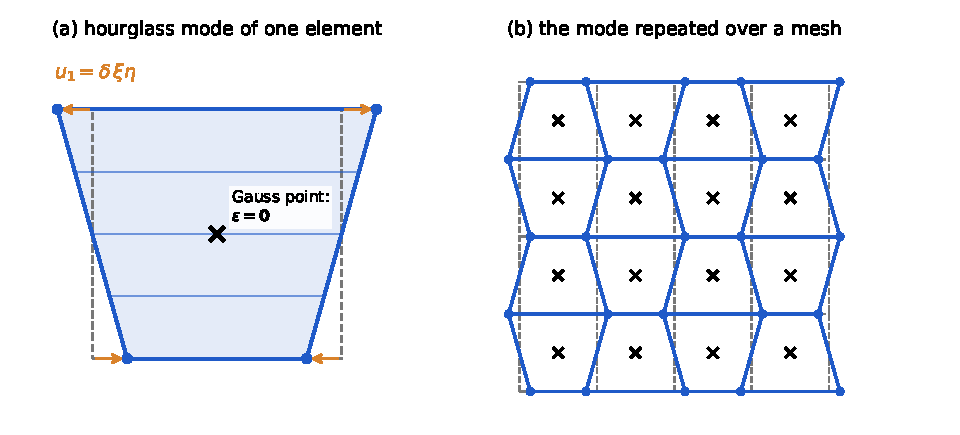
\includegraphics[width=0.85\textwidth]{figures/ch2/hourglass.pdf}
\caption{Hourglass mode of a bilinear square integrated with one Gauss point
(cross). (a) The nodal displacements $\pm\delta$ deform the element, but the
strain vanishes at the centre. (b) The same mode with alternating signs is a
zero-energy mode of the whole mesh.}
\label{fig:hourglass}
\end{figure}

\exercise{A bar in tension by the Ritz method}\label{exo:bar}
A bar of length $L$, section $A$ and modulus $E$ is clamped at $x=0$, loaded by
a uniform axial force $f$ per unit length and by a force $F$ at $x=L$. (a) Write
the potential energy and the exact solution. (b) Ritz with $w_1=x$. (c) Ritz
with $w_1=x$, $w_2=x^2$. Compare the end displacements and the energies.
\begin{solution}
(a) $\displaystyle \mathcal U_p(v)=\int_0^L\tfrac12EA(v')^2-\int_0^Lfv-Fv(L)$, $v(0)=0$;
Euler--Lagrange: $-EAu''=f$, $EAu'(L)=F$, so
$\displaystyle u=\frac{(F+fL)x-fx^2/2}{EA}$, $\displaystyle u(L)=\frac{FL+fL^2/2}{EA}$.
(b) $v=\alpha x$: $\mathcal U_p=\tfrac12EAL\alpha^2-\alpha(fL^2/2+FL)$, so
$\alpha=(F+fL/2)/EA$ and $v(L)=u(L)$ exactly, but the strain $\alpha$ is
constant: the stress is the average of the exact one. The energy is higher
than the exact one by $\displaystyle \frac{f^2L^3}{24EA}$.
(c) The exact solution belongs to the trial space, so the Ritz method
returns it: the Ritz solution is the best approximation in energy norm.
Figure~\ref{fig:bar-ritz} shows the three solutions for $F=0$: the
one-term displacement is exact only at the end, and its constant normal
force is the average of the exact one.
\end{solution}
\begin{figure}[h]
\centering
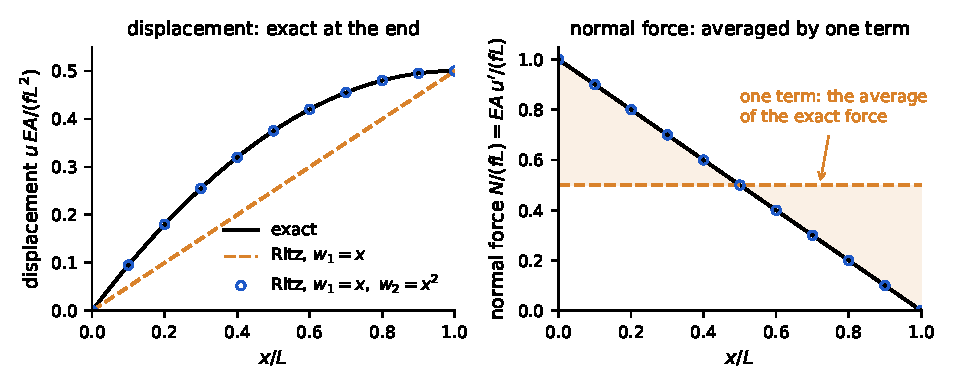
\includegraphics[width=0.9\textwidth]{figures/ch2/bar_ritz.pdf}
\caption{Ritz solutions of the bar of Exercise~\ref{exo:bar} under a uniform
load $f$, free end ($F=0$). Left: displacement. Right: normal force
$N=EA\,u'$. One term ($w_1=x$) gives a constant force, the average of the
exact one; two terms ($w_1=x$, $w_2=x^2$) give the exact solution.}
\label{fig:bar-ritz}
\end{figure}

\exercise{Why not polynomials?}\label{exo:conditioning}
For the bar of Exercise~\ref{exo:bar} with $EA=L=1$, use the monomials
$w_m=x^m$, $m=1,\dots,n$. Compute $\displaystyle K_{m\ell}=\int_0^1w_m'w_\ell'$ and its
condition number for $n=3,5,7,9$. Compare with $n$ hat functions.
\begin{solution}
$K_{m\ell}=m\ell/(m+\ell-1)$, a Hilbert-like matrix. Its condition numbers are
\begin{center}\renewcommand{\arraystretch}{1.1}
\begin{tabular}{lcccc}
\toprule
$n$ & 3 & 5 & 7 & 9\\
\midrule
monomials $x^m$ & $2.8\times10^2$ & $1.9\times10^5$ & $1.7\times10^8$ & $1.6\times10^{11}$\\
hat functions & $16.4$ & $45.5$ & $87.6$ & $142.7$\\
\bottomrule
\end{tabular}
\end{center}
\lstinputlisting[firstline=4]{python/examples/ch2/exo_conditioning.py}
The condition number of the monomial basis grows geometrically, by a factor
of about $30$ per function: from $n=12$ on it exceeds the inverse of the
machine precision, and the computed coefficients are meaningless
(Figure~\ref{fig:conditioning}). That of the finite element basis grows like
$1/h^2=n^2$.
\begin{figure}[h]
\centering
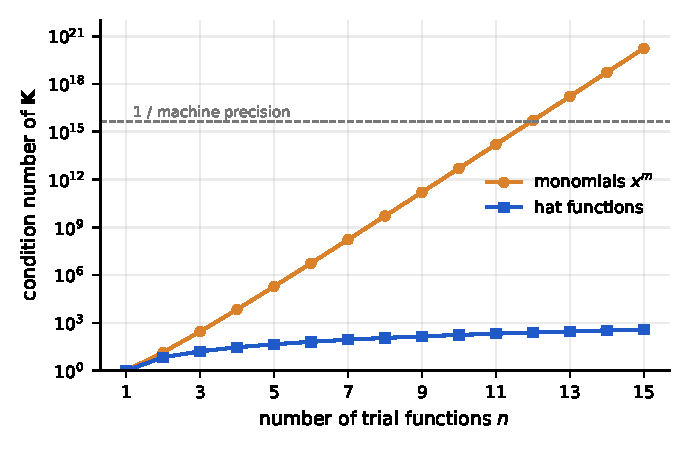
\includegraphics[width=0.6\textwidth]{figures/ch2/conditioning.pdf}
\caption{Condition number of the stiffness matrix of the bar against the
number of trial functions: monomials (geometric growth) and hat functions
(growth like $n^2$). Dashed: the inverse of the double-precision machine
epsilon.}
\label{fig:conditioning}
\end{figure}
\end{solution}

\exercise{A plate with a hole: Kirsch against finite elements}\label{exo:kirsch}
\index{Kirsch problem}\index{stress concentration}\index{finite element method!test against a closed-form solution}%
An infinite plate with a circular hole of radius $a$ carries a remote uniaxial
tension $\sigma$ along $\ve_1$ (plane stress or plane strain). In polar
coordinates $(r,\theta)$, with $\theta$ measured from $\ve_1$, the solution of
Kirsch~\cite{Kirsch1898} is
\begin{align*}
  \sigma_{rr}&=\frac\sigma2\Bigl(1-\frac{a^2}{r^2}\Bigr)
  +\frac\sigma2\Bigl(1-4\frac{a^2}{r^2}+3\frac{a^4}{r^4}\Bigr)\cos2\theta,\\
  \sigma_{\theta\theta}&=\frac\sigma2\Bigl(1+\frac{a^2}{r^2}\Bigr)
  -\frac\sigma2\Bigl(1+3\frac{a^4}{r^4}\Bigr)\cos2\theta,\qquad
  \sigma_{r\theta}=-\frac\sigma2\Bigl(1+2\frac{a^2}{r^2}-3\frac{a^4}{r^4}\Bigr)\sin2\theta .
\end{align*}
(a) Check the boundary conditions on the hole and at infinity. Give
$\sigma_{\theta\theta}$ on the hole and the stress concentration factor.
(b) Give $\sigma_{11}$ on the ligament $x_1=0$. At which distance from the hole
is it within $10\%$ of $\sigma$?
(c) Write a finite element program with linear triangles for a quarter of a
square plate of side $40a$: symmetry conditions $u_1=0$ on $x_1=0$ and $u_2=0$
on $x_2=0$, traction $\sigma\ve_1$ on the edge $x_1=20a$, a mesh graded
towards the hole. Compare with Kirsch on the hole and on the ligament, and
refine the mesh.
(d) Repeat the computation with a general finite element code, for instance
Cast3M or FEniCS, with linear and quadratic triangles, and compare the
meshes needed for a $1\%$ accuracy on the concentration factor.
\begin{solution}
(a) At $r=a$: $\sigma_{rr}=\tfrac\sigma2(1-4+3)\cos2\theta=0$ and
$\sigma_{r\theta}=-\tfrac\sigma2(1+2-3)\sin2\theta=0$: the hole is free. As
$r\to\infty$: $\sigma_{rr}\to\sigma\cos^2\theta$,
$\sigma_{\theta\theta}\to\sigma\sin^2\theta$,
$\sigma_{r\theta}\to-\sigma\sin\theta\cos\theta$, the polar components of
$\sigma\,\ve_1\otimes\ve_1$. On the hole
$\sigma_{\theta\theta}=\sigma(1-2\cos2\theta)$: $-\sigma$ at $\theta=0$ and
$3\sigma$ at $\theta=\pm\tfrac\pi2$. The concentration factor is $3$,
independent of the radius and of the elastic constants.
(b) On $x_1=0$, $\theta=\tfrac\pi2$ and $\sigma_{11}=\sigma_{\theta\theta}
=\sigma\bigl(1+\tfrac12a^2/x_2^2+\tfrac32a^4/x_2^4\bigr)$. With $t=a^2/x_2^2$,
$\tfrac12t+\tfrac32t^2=0.1$ gives $t=0.141$, $x_2=2.7a$: the perturbation
is local (Saint-Venant).
(c) The program below meshes the quarter plate with $n_\theta$ cells along
the hole and cells of nearly square shape growing geometrically away from it,
assembles the stiffness of linear triangles in plane stress, and averages the
element stresses at the nodes. It prints
\begin{center}\renewcommand{\arraystretch}{1.1}
\begin{tabular}{lcccc}
\toprule
$n_\theta$ & 12 & 24 & 48 & 96\\
\midrule
degrees of freedom & 624 & 2352 & 9120 & 35712\\
$\sigma_{11}(0,a)/\sigma$ (Kirsch: $3$) & 2.970 & 3.013 & 3.020 & 3.021\\
$\sigma_{22}(a,0)/\sigma$ (Kirsch: $-1$) & $-0.722$ & $-0.871$ & $-0.946$ & $-0.982$\\
\bottomrule
\end{tabular}
\end{center}
The concentration factor converges to $3.02$, not $3$: the plate is finite.
With a side of $160a$ the same mesh density gives $3.00$. The compressive
value at $\theta=0$ converges more slowly: there the hoop stress drops from
$-\sigma$ to $-0.6\sigma$ within $0.1a$, and the nodal average of constant
element stresses smooths this gradient. Figure~\ref{fig:kirsch} compares the
fields for $n_\theta=48$.
\lstinputlisting[firstline=4]{python/examples/ch2/kirsch_fem.py}
(d) Both codes follow the same steps: mesh, symmetry conditions, traction on
the edge, solution, nodal stresses on the hole. Quadratic triangles represent
the linear variation of the stress inside each element, and reach the same
accuracy with far fewer degrees of freedom.
\end{solution}
\begin{figure}[h]
\centering
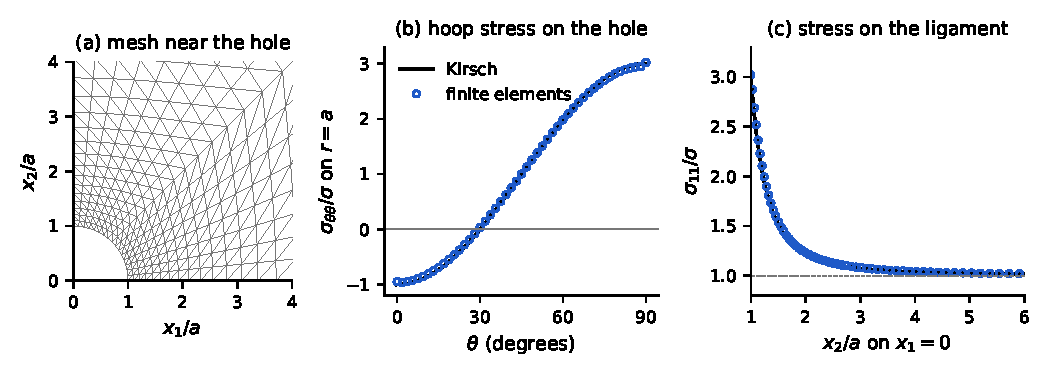
\includegraphics[width=\textwidth]{figures/ch2/kirsch.pdf}
\caption{Plate with a hole under remote tension $\sigma$ (Exercise~\ref{exo:kirsch}),
linear triangles, $48$ cells along the quarter hole. (a) The mesh near the
hole (shown coarser). (b) Hoop stress on the hole: from $-\sigma$ to the
concentration $3\sigma$. (c) $\sigma_{11}$ on the ligament $x_1=0$: the
perturbation decays within a few radii.}
\label{fig:kirsch}
\end{figure}

%======================================================================
\begin{chapterbib}{99}
\bibitem{BonnetFrangi2007} M.~Bonnet, A.~Frangi, \emph{Analyse des solides d\'eformables par la m\'ethode des \'el\'ements finis}, \'Editions de l'\'Ecole Polytechnique, 2007.
\bibitem{Chadwick2001} P.~Chadwick, M.~Vianello, S.~C.~Cowin, A new proof that the number of linear elastic symmetries is eight, \emph{J. Mech. Phys. Solids} 49 (2001) 2471--2492.
\bibitem{Coirier1997} J.~Coirier, \emph{M\'ecanique des milieux continus}, Dunod, 1997.
\bibitem{Crank1975} J.~Crank, \emph{The Mathematics of Diffusion}, 2nd ed., Oxford University Press, 1975.
\bibitem{ConstantinescuKorsunsky2007} A.~Constantinescu, A.~Korsunsky, \emph{Elasticity with Mathematica}, Cambridge University Press, 2007.
\bibitem{CottrellHughesBazilevs2009} J.~A.~Cottrell, T.~J.~R.~Hughes, Y.~Bazilevs, \emph{Isogeometric Analysis: Toward Integration of CAD and FEA}, Wiley, 2009.
\bibitem{FreezeCherry} R.~A.~Freeze, J.~A.~Cherry, \emph{Groundwater}, Prentice-Hall, 1979.
\bibitem{Germain1983} P.~Germain, \emph{M\'ecanique des milieux continus}, Masson, 1983.
\bibitem{HughesCottrellBazilevs2005} T.~J.~R.~Hughes, J.~A.~Cottrell, Y.~Bazilevs, Isogeometric analysis: CAD, finite elements, NURBS, exact geometry and mesh refinement, \emph{Comput. Methods Appl. Mech. Engrg.} 194 (2005) 4135--4195.
\bibitem{Hughes1987} T.~J.~R.~Hughes, \emph{The Finite Element Method}, Prentice Hall, 1987.
\bibitem{IncroperaDeWitt} F.~P.~Incropera, D.~P.~DeWitt, T.~L.~Bergman, A.~S.~Lavine, \emph{Fundamentals of Heat and Mass Transfer}, 6th ed., Wiley, 2007.
\bibitem{Kirsch1898} E.~G.~Kirsch, Die Theorie der Elastizit\"at und die Bed\"urfnisse der Festigkeitslehre, \emph{Zeitschrift des Vereines deutscher Ingenieure} 42 (1898) 797--807.
\bibitem{Nye1985} J.~F.~Nye, \emph{Physical Properties of Crystals: Their Representation by Tensors and Matrices}, Oxford University Press, 1957; revised edition 1985.
\bibitem{Salencon2001} J.~Salen\c{c}on, \emph{Handbook of Continuum Mechanics: General Concepts, Thermoelasticity}, Springer, 2001.
\bibitem{SoutasLittle1973} R.~W.~Soutas-Little, \emph{Elasticity}, Dover, 1973.
\bibitem{StrangAM} G.~Strang, \emph{Introduction to Applied Mathematics}, Wellesley-Cambridge Press, 1986.
\end{chapterbib}

%======================================================================
\chapter{Identification of a planar crack by the reciprocity gap}\label{ch:rg}
%======================================================================
% Source: rg_crack_theory.tex (electrostatics), notes C1 Section 4.

\framepart{Outline}
This chapter considers the identification of a planar crack in a conducting body from overdetermined boundary data. After stating the direct problem and its well-posedness, we formulate the inverse problem and review what is known about its uniqueness and stability. The reciprocity gap turns the overdetermined data into linear functionals of the crack opening. For a planar crack, these functionals give the crack in three explicit steps, following Andrieux and Ben Abda: the normal, the plane and the extension. We present these steps in three dimensions, with the double sine--sinh form of the extension formula and its stability. Two variants of the extension step follow: polynomial adjoint fields, which give the moments of the opening, and a dipole estimate based on the polarization tensor of a crack (Ammari and Kang). We then explain how several experiments are combined. The two-dimensional versions used in the numerical codes are collected in the last section.

\paragraph{By the end of this chapter you should be able to:}
\begin{itemize}
  \item state the direct problem of a cracked conducting body and prove its
  well-posedness, and formulate the inverse problem with overdetermined data;
  \item derive the reciprocity gap identity from Green's second identity and
  choose adjoint fields that extract given information on the crack;
  \item reconstruct the normal, the plane and the extension of a planar
  crack, and explain why the last step is only logarithmically stable;
  \item size a crack from its dipole moment, and combine several
  experiments into an optimal virtual experiment.
\end{itemize}

\paragraph{Plan of the chapter.} Sections~\ref{sec:rg-direct}--\ref{sec:rg-inverse} state the direct and inverse problems, and Section~\ref{sec:rg-lit} reviews uniqueness and stability results. Section~\ref{sec:rg-gap} introduces the reciprocity gap. Section~\ref{sec:rg-rec} gives the reconstruction of a planar crack in three dimensions, its stability, and two variants of the extension step. Section~\ref{sec:rg-multi} explains how several experiments are combined, Section~\ref{sec:rg-num} gathers the two-dimensional formulas used in the numerical codes, and a summary, exercises with solutions (page~\pageref{sec:rg-exo}) and the references close the chapter.

\begin{gbox}{Guiding questions}
Overspecified boundary data, where the potential \emph{and} the flux are known
on the boundary from a single physical measurement, let one probe for a hidden
defect. The chapter answers, in order, the following questions.
\begin{enumerate}[itemsep=1pt]
  \item What is a crack, mathematically? Here: an unknown surface $\Gamma$
  across which no flux passes, an insulating (or traction-free) crack.
  \item What are the strong and weak formulations for the cracked body
  $\Omega\setminus\Gamma$? (Section~\ref{sec:rg-direct})
  \item Which reciprocity equation relates the unknown cracked body and a
  fictitious uncracked body occupying the same $\Omega$?
  (Section~\ref{sec:rg-gap})
  \item What can be deduced about $\Gamma$ from this equation alone, and can
  particular fictitious fields extract its plane, its position and its size?
  (Sections~\ref{sec:rg-rec}--\ref{sec:rg-multi})
\end{enumerate}
The tools are those of Chapters~\ref{ch:var} and~\ref{ch:elliptic}: the
weak form and Lax--Milgram for the direct problem, Green's second identity
(Appendix~\ref{app:ibp}) for reciprocity, and the scalar diffusion problem of
Section~\ref{sec:diff}, which is also anti-plane elasticity
(Exercise~\ref{exo:antiplane}).
\end{gbox}

\section{Introduction}\label{sec:rg-intro}
\index{crack!insulating}\index{crack!identification}\index{non-destructive evaluation}%
The problem studied here is a scalar, stationary diffusion problem: a potential $u$ drives a flux $\vq=-\bbK\nabla u$ that is conserved, $\operatorname{div}\vq=0$, in a body with the tensor of diffusion coefficients $\bbK$ of Chapter~\ref{ch:elliptic}. A crack is a surface across which no flux passes, $\vq\cdot\vn=0$ on both lips, while the potential may jump. The same mathematical problem arises in several physical settings (Table~\ref{tab:rg-phys}).

\begin{table}[h]
\centering\small
\renewcommand{\arraystretch}{1.15}
\begin{tabular}{>{\raggedright}p{2.6cm}>{\raggedright}p{2.3cm}>{\raggedright}p{2.6cm}>{\raggedright}p{2.6cm}>{\raggedright\arraybackslash}p{3.7cm}}
\toprule
\sffamily setting & \sffamily potential $u$ & \sffamily flux $\vq$ & \sffamily crack & \sffamily typical measurement\\
\midrule
electrostatics, steady currents & electric potential & current density & insulating crack & electrodes; potential drop\\
heat conduction & temperature & heat flux & adiabatic crack, delamination & thermocouples, infrared camera\\
porous media (Darcy) & hydraulic head, pressure & Darcy velocity & impermeable fault or barrier & pumping and observation wells\\
mass diffusion (Fick) & concentration & diffusive flux & impermeable barrier & sampling at the boundary\\
anti-plane elasticity & out-of-plane displacement & shear stress $\sigma_{3i}$ & traction-free mode~III crack & displacement and traction measurements\\
\bottomrule
\end{tabular}
\caption{Physical interpretations of the model problem $\operatorname{div}(k\nabla u)=0$ with a zero-flux crack.}
\label{tab:rg-phys}
\end{table}

\paragraph{Applications.} In each of these settings, crack identification from boundary measurements is a practical question.
\begin{itemize}[itemsep=1pt]
\item \emph{Electrical potential drop methods.} A current is driven through a metallic component and the potential is measured near a surface crack to size it. This is a standard technique of non-destructive evaluation; its analysis uses Green's theorem for the Laplace equation, as here~\cite{IYM91}. Electrostatic data were also the original motivation of the mathematical crack problem~\cite{FV89,SV91}.
\item \emph{Thermal methods.} Active infrared thermography detects delaminations and cracks in composite and metallic parts. The stationary limit of the heat equation is the present problem, and the reciprocity gap extends to transient heat diffusion~\cite{BCM05}.
\item \emph{Porous media.} In hydrogeology and reservoir engineering, impermeable (sealing) faults are inferred from pressure measurements in wells. The steady Darcy problem with an impermeable fault is the present problem; boundary data are, however, usually available only at a few wells.
\item \emph{Elasticity.} Anti-plane shear is the simplest elastic case. The reciprocity gap method extends to linear elasticity~\cite{ABB99} and to elastodynamics~\cite{BCM04,BCM05}.
\end{itemize}


%======================================================================
\section{The direct problem}\label{sec:rg-direct}
\index{direct problem!cracked body}\index{well-posedness}%
Let $\Omega\subset\R^3$ be a bounded, connected Lipschitz domain with outward unit normal $\vnu$. The crack $\Gamma\subset\Omega$ is a closed, bounded planar domain with Lipschitz boundary $\partial\Gamma$ (the crack front), lying in the plane $\Pi=\{\vx:\ \vn\cdot\vx=c\}$. Its two lips are $\Gamma^+$, on the side towards which $\vn$ points, and $\Gamma^-$. We write $\OG=\Omega\setminus\Gamma$; it is connected because $\Gamma$ is compactly contained in $\Omega$. To simplify, the body is homogeneous and isotropic, and the potential is scaled so that $\bbK=\tI$: the balance $\dive(\bbK\nabla u)=0$ becomes the Laplace equation $\Delta u=0$, and the flux through a surface of normal $\vnu$ is $\partial_\nu u=\nabla u\cdot\vnu$. As in Chapter~\ref{ch:elliptic}, the boundary is split into two complementary parts (Figure~\ref{fig:rg-problems}a): the potential is prescribed on $S_u$ (electrodes) and the flux on $S_\varphi$.

\begin{figure}[h]
\centering
% Chapter 3, direct and inverse problems (Sections 3.2-3.3), in the style of
% fig:3Dbody. (a) complementary data: u = u^D on S_u, flux on S_phi, crack
% known. (b) overdetermined data: u and its normal derivative known on the
% whole boundary (two offset contours), crack unknown.
\begin{tikzpicture}[scale=0.9,>={Latex[length=2mm]}]
\def\blob{(A) to[out=-70,in=180] (B) to[out=0,in=-130] (C)
    to[out=50,in=-30] (D) to[out=150,in=10] (E) to[out=190,in=110] (A)}
\tikzset{body/.style={fill=gray!12},
  crack/.style={line width=1.8pt,line cap=round}}
% ---------------- (a) direct problem ----------------
\begin{scope}
  \coordinate (A) at (0,0.6);   \coordinate (B) at (2.0,-0.4);
  \coordinate (C) at (4.4,0.5); \coordinate (D) at (3.9,2.6);
  \coordinate (E) at (1.0,2.5);
  % S_u (electrodes, blue) and S_phi (flux, green)
  \draw[cu!30,line width=6pt] (E) to[out=190,in=110] (A) to[out=-70,in=180] (B);
  \fill[body] \blob -- cycle;
  \draw[cu,very thick] (E) to[out=190,in=110] (A) to[out=-70,in=180] (B);
  \draw[cphi,very thick,postaction={decorate},decoration={markings,
     mark=at position 0.80 with {\draw[->,thick,black] (0,0) -- (0,-0.75) coordinate (N);}}]
    (B) to[out=0,in=-130] (C) to[out=50,in=-30] (D) to[out=150,in=10] (E);
  \node[left] at (N) {$\vnu$};
  % the crack, known
  \draw[crack] (1.75,1.05) -- (2.85,1.6);
  \node[below right=-1pt] at (2.55,1.45) {$\Gamma$};
  \node at (1.35,1.75) {$\Delta u=0$};
  \node[cu,anchor=north east,align=right,font=\small] at (1.05,-0.4)
    {$S_u$: $u=\uD$};
  \node[cphi,anchor=west,align=left,font=\small] at (4.75,1.75)
    {$S_\varphi$:\\ $\partial_\nu u=\pD$};
  \node[font=\sffamily] at (2.2,-1.35) {(a) direct problem};
\end{scope}
% ---------------- (b) inverse problem ----------------
\begin{scope}[xshift=8.0cm]
  \coordinate (A) at (0,0.6);   \coordinate (B) at (2.0,-0.4);
  \coordinate (C) at (4.4,0.5); \coordinate (D) at (3.9,2.6);
  \coordinate (E) at (1.0,2.5);
  % two offset contours: u known (blue, inner), flux known (green, outer)
  \draw[cphi,line width=8pt,line join=round] \blob -- cycle;
  \draw[white,line width=5.4pt,line join=round] \blob -- cycle;
  \draw[cu,line width=3.2pt,line join=round] \blob -- cycle;
  \fill[body] \blob -- cycle;
  \draw[gray!50!black,thin] \blob -- cycle;
  % the crack, unknown
  \draw[crack,red!70!black,dash pattern=on 4pt off 2.5pt,line cap=butt]
    (1.75,1.05) -- (2.85,1.6);
  \node[red!70!black,below right=-1pt] at (2.55,1.45) {$\Gamma\,?$};
  \node at (1.35,1.75) {$\Delta u=0$};
  \draw[cu,thin] (0.45,2.25) -- (-0.15,2.75) node[above left=-2pt,font=\small]
    {$u=\uD$ on $\partial\Omega$};
  \draw[cphi,thin] (3.95,-0.05) -- (4.5,-0.45) node[below right=-2pt,font=\small]
    {$\partial_\nu u=\pD$ on $\partial\Omega$};
  \node[font=\sffamily] at (2.2,-1.35) {(b) inverse problem};
\end{scope}
\end{tikzpicture}

\caption{(a) Direct problem: complementary boundary conditions; the potential
is given on $S_u$ (blue) and the flux on $S_\varphi$ (green), and the crack
$\Gamma$ is known. (b) Inverse problem: overspecified, overlapping boundary
conditions; after the measurements both the potential and the flux are known
on the boundary, and the crack is unknown. Compare with the elastic body of
Figure~\ref{fig:3Dbody}.}
\label{fig:rg-problems}
\end{figure}

\begin{gbox}{Direct problem}
Given $\Gamma$, a partition $\partial\Omega=\overline{S_u}\cup\overline{S_\varphi}$, $S_u\cap S_\varphi=\emptyset$, and boundary data $\uD$ on $S_u$, $\pD$ on $S_\varphi$, find $u$ such that
\begin{equation}\label{eq:rg-direct}
\left\{\begin{aligned}
\Delta u&=0 &&\text{in }\OG,\\
\partial_n u^\pm&=0 &&\text{on }\Gamma^\pm,\\
u&=\uD &&\text{on }S_u,\\
\partial_\nu u&=\pD &&\text{on }S_\varphi .
\end{aligned}\right.
\end{equation}
\end{gbox}

\paragraph{Well-posedness.}
\index{well-posedness!in the sense of Hadamard}%
A problem is \emph{well posed in the sense of Hadamard} if it has a
solution, if this solution is unique, and if it depends continuously on the
data: a small change of the data gives a small change of the solution
(stability). ``Small'' is measured with the energy. The potential has a
finite energy, $u\in H^1(\OG)$. Its boundary values then belong to
$H^{1/2}$: this is the space of the traces of the fields of finite energy,
i.e.\ of the boundary potentials that a field of finite energy can take. A
potential that jumps along a line of the boundary, for instance, is not in
$H^{1/2}$: no field of finite energy takes it. The fluxes belong to the dual
space $\tilde H^{-1/2}(S_\varphi)$, the dual of $H^{1/2}_{00}(S_\varphi)$: the
fluxes whose power $\displaystyle \int_{S_\varphi}\pD v\dd s$ against these boundary
potentials is finite. With $|S_u|>0$, $\uD\in H^{1/2}(S_u)$ and
$\pD\in\tilde H^{-1/2}(S_\varphi)$, problem~\eqref{eq:rg-direct} has a unique
weak solution $u\in H^1(\OG)$, and
\begin{equation}\label{eq:rg-stab-direct}
\|u\|_{H^1(\OG)}\le C\bigl(\|\uD\|_{H^{1/2}(S_u)}+\|\pD\|_{\tilde H^{-1/2}(S_\varphi)}\bigr),
\end{equation}
with $C$ depending only on $\Omega$, $\Gamma$ and $S_u$: the direct problem is well posed in the sense of Hadamard.

To see this, let $V=\{v\in H^1(\OG):\ v=0\text{ on }S_u\}$, and let $U\in H^1(\Omega)$ be a lifting of $\uD$. The weak form is to find $w=u-U\in V$ such that
\[
\int_{\OG}\nabla w\cdot\nabla v\,d\vx=\langle\pD,v\rangle_{S_\varphi}-\int_{\OG}\nabla U\cdot\nabla v\,d\vx\qquad\forall v\in V .
\]
The zero-flux conditions on the lips and the flux on $S_\varphi$ are natural conditions of this form. $\OG$ is connected and is the union of two Lipschitz subdomains, obtained by cutting $\Omega$ along a surface that extends $\Gamma$ to $\partial\Omega$. The Poincaré--Friedrichs inequality therefore holds on $V$ because $|S_u|>0$, so the bilinear form is coercive. The Lax--Milgram lemma (Section~\ref{sec:var-lm}) gives existence, uniqueness and~\eqref{eq:rg-stab-direct}, exactly as for the diffusion problem of Section~\ref{sec:diff}.

\paragraph{Pure flux data.} If $S_u=\emptyset$, a solution exists if and only if $\displaystyle \int_{\partial\Omega}\pD\,ds=0$, and it is unique up to an additive constant; \eqref{eq:rg-stab-direct} holds in $H^1(\OG)/\R$.

\paragraph{Behaviour at the crack front.} Near $\partial\Gamma$, $u$ behaves like $r^{1/2}\cos(\theta/2)$ in polar coordinates in the plane normal to the front. The opening $\jump u=u^+-u^-$ therefore vanishes like the square root of the distance to the front, and its extension by zero to $\Pi$ belongs to $H^{1/2}(\Pi)$: $\jump u\in\tilde H^{1/2}(\Gamma)$.
\index{crack!front singularity}%

%======================================================================
\section{The inverse problem}\label{sec:rg-inverse}
\index{inverse problem}\index{inverse problem!overdetermined data}\index{Cauchy data}\index{ill-posed problem}%
In the inverse problem the crack $\Gamma$ is unknown. To recover it we add information by overspecifying the boundary conditions. The experiment imposes the potential on a part of the boundary and the flux on the rest, as in the direct problem, and it also measures the flux where the potential is imposed (the current through the electrodes) and the potential where the flux is imposed. After the experiment the potential is known on $S_u$ and the flux on $S_\varphi$, but $S_u$ and $S_\varphi$ are not complementary any more: they overlap on $\Sigma=S_u\cap S_\varphi\neq\emptyset$ (Figure~\ref{fig:rg-problems}b).

\begin{gbox}{Inverse problem}
Identify $\Gamma$ from the knowledge of the measured data $(\uD_k,\pD_k)$ of one or several experiments $k=1,\dots,K$. The solution $u_k$ of each experiment satisfies
\[
\Delta u_k=0\ \text{in }\OG,\qquad \partial_nu_k^\pm=0\ \text{on }\Gamma^\pm,\qquad
u_k=\uD_k\ \text{on }S_u,\qquad \partial_\nu u_k=\pD_k\ \text{on }S_\varphi,
\]
where the boundary parts overlap: $\Sigma=S_u\cap S_\varphi\neq\emptyset$.
\end{gbox}

On $\Sigma$ both the potential and the flux are known: the data are \emph{overdetermined}, and this redundancy carries the information on $\Gamma$. We use mostly \emph{complete} overdetermined data, $S_u=S_\varphi=\partial\Omega$. This is the setting of~\cite{AB96}, and the situation of the numerical experiments, where the flux is measured on the electrodes and the potential on the insulated parts. When the data are incomplete, the missing data can first be reconstructed by solving a Cauchy problem for the Laplace equation near the boundary, for instance by the energy-gap method of~\cite{ABB06}; this step is itself ill-posed.

The map from $\Gamma$ to the data is nonlinear, and its inverse is unstable: smooth data perturbations may correspond to large changes of the crack. The inverse problem is ill-posed: it fails the third condition of Hadamard. Its stable solution needs a priori information or a regularization, in the sense of Tikhonov~\cite{TA77}; here the a priori information is the planarity of the crack.

%======================================================================
\section{Identifiability, uniqueness and stability: literature and ideas}\label{sec:rg-lit}
\paragraph{Blind experiments.} A single experiment cannot determine an arbitrary crack. Let $u_0$ be the solution of~\eqref{eq:rg-direct} without crack. If $\partial_n u_0=0$ on $\Gamma$, i.e.\ if the crack lies along the flux lines of $u_0$, then $u_0$ also solves the cracked problem. The crack does not change the data and is invisible. For a uniform field $\vE$ this happens when $\vE\cdot\vn=0$.
\index{blind experiment}%

\paragraph{Uniqueness.} Friedman and Vogelius~\cite{FV89} proved that two suitably chosen measurements determine an insulating crack, and gave stability results. Uniqueness was extended to a finite collection of cracks with two measurements by Kim and Seo~\cite{KS96} and by Alessandrini and Diaz Valenzuela~\cite{ADV96}. For three-dimensional cracks, Eller~\cite{Ell96} obtained identification from many boundary measurements. For a planar crack, the inversion formulae of Andrieux and Ben Abda~\cite{AB96} give a constructive proof: one non-blind experiment with complete data determines the crack (Section~\ref{sec:rg-rec}).
\index{inverse problem!uniqueness}%

\paragraph{Stability.} The dependence of the crack on the data is in general only logarithmic~\cite{Ale93}. Under a priori restrictions the stability improves: for linear cracks it becomes Lipschitz~\cite{ABV96}. The logarithmic resolution found for the extension step in Section~\ref{ssec:rg-stab} is a concrete instance of this ill-posedness.
\index{inverse problem!stability}\index{stability!logarithmic}%

\paragraph{Reconstruction methods.} Iterative methods minimise a misfit over crack geometries~\cite{SV91,BV94}. Sampling and factorization methods characterise the crack through the range of a data operator~\cite{BHP01}. Direct methods, such as the reciprocity gap used here~\cite{AB96,ABB99,BCM04,BCM05}, compute geometric quantities in closed form. Asymptotic methods treat the defect as a small inhomogeneity and use its polarization tensor~\cite{AK04}. The review~\cite{BV04} surveys these works.

%======================================================================
\section{The reciprocity gap}\label{sec:rg-gap}
\index{reciprocity gap}\index{reciprocity!gap}\index{adjoint field}%
Let $u$ solve~\eqref{eq:rg-direct} for the unknown crack, with complete Cauchy data $(u,\varphi)$ on $\partial\Omega$, $\varphi=\partial_\nu u$. An \emph{adjoint field} $v$ is a function harmonic in the whole domain $\Omega$, without crack. We choose it, usually in closed form, so $v$ and $\partial_\nu v$ are known on $\partial\Omega$ (Figure~\ref{fig:rg-rg}).

\paragraph{An identity between the boundary and the crack.} For every adjoint field $v$, smooth near $\Gamma$,
\begin{equation}\label{eq:rg-identity}
\int_{\partial\Omega}\bigl(u\,\partial_\nu v-v\,\partial_\nu u\bigr)\,ds=\int_\Gamma\jump u\,\partial_nv\,ds,\qquad \jump u=u^+-u^- .
\end{equation}
It follows from an integration by parts and from $\Delta v=0$. Green's second identity in the cut domain $\OG$ (Appendix~\ref{app:ibp}) reads
\[
\int_{\OG}\bigl(v\,\Delta u-u\,\Delta v\bigr)\,d\vx=\int_{\partial\OG}\bigl(v\,\partial_{\nu'}u-u\,\partial_{\nu'}v\bigr)\,ds,
\]
where $\nu'$ is the outward normal of $\OG$. The left-hand side vanishes, since $\Delta u=0$ in $\OG$ and $\Delta v=0$ in $\Omega$. The boundary $\partial\OG$ consists of $\partial\Omega$, where $\nu'=\vnu$, and of the two lips, where $\nu'=-\vn$ on $\Gamma^+$ and $\nu'=+\vn$ on $\Gamma^-$ (Figure~\ref{fig:lips}). On the lips $\partial_{\nu'}u=0$, while $v$ and $\partial_nv$ are single-valued because $v$ is smooth across $\Gamma$. The lips therefore contribute $\displaystyle \int_\Gamma(u^+-u^-)\,\partial_nv\,ds$, and
$\displaystyle 0=\int_{\partial\Omega}(v\,\partial_\nu u-u\,\partial_\nu v)\,ds+\int_\Gamma\jump u\,\partial_nv\,ds$, which is~\eqref{eq:rg-identity}.

The left-hand side of~\eqref{eq:rg-identity} uses only the boundary data and the chosen field $v$; the right-hand side only the crack and its opening. It deserves a name.

\begin{gbox}{Reciprocity gap}
For every $v\in\mathcal H(\Omega)=\{v\in H^1(\Omega):\ \Delta v=0\text{ in }\Omega\}$, smooth near $\Gamma$, the reciprocity gap of the data $(u,\varphi)$ is
\begin{equation}\label{eq:rg-rgdef}
\RG(v)=\int_{\partial\Omega}\bigl(u\,\partial_\nu v-v\,\varphi\bigr)\,ds ,
\end{equation}
and, by~\eqref{eq:rg-identity},
\begin{equation}\label{eq:rg-rg}
\RG(v)=\int_\Gamma\jump u\,\partial_n v\,ds .
\end{equation}
\end{gbox}

\begin{figure}[h]
\centering
% Chapter 3, the reciprocity gap (Section 3.5), replaces the three rectangles
% of fig:rg-rg. (a) the cracked body with its measured Cauchy data (u and
% phi = d_nu u on the whole boundary), the crack Gamma, its normal n and
% lips. (b) an adjoint field v, harmonic in the uncracked body, with v and
% d_nu v known on the boundary. The reciprocity gap pairs the two.
\begin{tikzpicture}[scale=0.9,>={Latex[length=2mm]}]
\def\blob{(A) to[out=-70,in=180] (B) to[out=0,in=-130] (C)
    to[out=50,in=-30] (D) to[out=150,in=10] (E) to[out=190,in=110] (A)}
\tikzset{body/.style={fill=gray!12},
  crack/.style={line width=1.8pt,line cap=round}}
\def\cauchybody{%
  \coordinate (A) at (0,0.6);   \coordinate (B) at (2.0,-0.4);
  \coordinate (C) at (4.4,0.5); \coordinate (D) at (3.9,2.6);
  \coordinate (E) at (1.0,2.5);
  \draw[cphi,line width=8pt,line join=round] \blob -- cycle;
  \draw[white,line width=5.4pt,line join=round] \blob -- cycle;
  \draw[cu,line width=3.2pt,line join=round] \blob -- cycle;
  \fill[body] \blob -- cycle;
  \draw[gray!50!black,thin] \blob -- cycle;}
% ---------------- (a) cracked body, measured data ----------------
\begin{scope}
  \cauchybody
  \draw[crack] (1.75,1.05) -- (2.85,1.6);
  \draw[->,thick] (2.3,1.325) -- ++(-0.3,0.6) node[left=-1pt] {$\vn$};
  \node[above right=-2pt] at (2.65,1.5) {$\Gamma^+$};
  \node[below right=-1pt] at (2.2,1.3) {$\Gamma^-$};
  \node at (1.05,1.45) {$\OG$};
  \node at (3.15,0.55) {$\Delta u=0$};
  \draw[cu,thin] (0.45,2.25) -- (-0.15,2.75) node[above left=-2pt,font=\small] {$u$};
  \draw[cphi,thin] (0.35,0.0) -- (-0.15,-0.4) node[below left=-2pt,font=\small]
    {$\varphi=\partial_\nu u$};
  \node[font=\sffamily] at (2.2,-1.35) {(a) cracked body, measured data};
\end{scope}
% ---------------- (b) adjoint field ----------------
\begin{scope}[xshift=7.6cm]
  \cauchybody
  \node at (2.2,1.45) {$\Delta v=0$ in $\Omega$};
  \node[font=\small] at (2.2,0.95) {(no crack)};
  \draw[cu,thin] (4.05,2.3) -- (4.6,2.75) node[above right=-2pt,font=\small] {$v$};
  \draw[cphi,thin] (3.95,-0.05) -- (4.5,-0.45) node[below right=-2pt,font=\small]
    {$\partial_\nu v$};
  \node[font=\sffamily] at (2.2,-1.35) {(b) adjoint field};
\end{scope}
% ---------------- pairing ----------------
\draw[<->,thick,gray!60!black,shorten <=4pt,shorten >=4pt]
  (3.75,2.85) to[out=40,in=140]
  node[midway,above,black,font=\small]
    {$\displaystyle\RG(v)=\int_{\partial\Omega}(u\,\partial_\nu v-v\,\varphi)\dd s$}
  (7.6cm+0.9cm*1.15,2.85);
\end{tikzpicture}

\caption{The reciprocity gap. (a) The cracked body: after the experiment the
potential $u$ and the flux $\varphi=\partial_\nu u$ are known on the whole
boundary; the crack $\Gamma$, with normal $\vn$ and lips $\Gamma^\pm$, is
unknown. (b) An adjoint field $v$, harmonic in the uncracked body, with $v$
and $\partial_\nu v$ known on the boundary. The gap $\RG(v)$ pairs the
boundary data of (a) and (b).}
\label{fig:rg-rg}
\end{figure}

\paragraph{Reciprocity and its gap.} If there is no crack, $\RG(v)=0$ for all $v$: this is Betti--Maxwell reciprocity between the two harmonic fields $u$ and $v$, the continuum form of Proposition~\ref{prop:reciprocity}. The reciprocity gap measures how far the data are from those of an uncracked body, and~\eqref{eq:rg-rg} says that this distance is carried entirely by the opening of the crack. Each choice of $v$ tests the opening $\jump u$ against the function $\partial_nv$ on $\Gamma$; the families of adjoint fields of Section~\ref{sec:rg-rec} are chosen so that these tests give the normal, the plane and the shape of the crack.

\paragraph{Properties.}
\begin{enumerate}[label=(\roman*),itemsep=1pt]
\item The identity~\eqref{eq:rg-rg} holds for a curved crack as well, with $\vn$ the local normal.
\item $\RG$ is linear in $v$, and linear in the data $(u,\varphi)$. Linearity in the data is the basis of Section~\ref{sec:rg-multi}.
\item $|\RG(v)|\le\|u\|_{H^{1/2}(\partial\Omega)}\|\partial_\nu v\|_{H^{-1/2}(\partial\Omega)}+\|\varphi\|_{H^{-1/2}(\partial\Omega)}\|v\|_{H^{1/2}(\partial\Omega)}$. Data errors are amplified by the size of $v$ on $\partial\Omega$, which matters for the extension step.
\item As a distribution, $v\mapsto\RG(v)$ is the double layer of density $\jump u$ on $\Gamma$, tested on harmonic functions. Identifying the crack means identifying the support of this double layer.
\end{enumerate}

%======================================================================
\section{Reconstruction of a planar crack}\label{sec:rg-rec}
\index{crack!planar, reconstruction}\index{moments of the opening}%
From now on $\Gamma$ lies in the plane $\Pi=\{\vx:\ \vn\cdot\vx=c\}$, with in-plane unit vectors $\vt_1,\vt_2$ such that $(\vt_1,\vt_2,\vn)$ is a direct orthonormal basis. Following~\cite{AB96}, the crack is obtained in three steps, each with a family of adjoint fields in~\eqref{eq:rg-rg}. We write
\[
m_0=\int_\Gamma\jump u\,ds
\]
and assume $m_0\ne0$. This holds for every non-blind experiment in a uniform field (Section~\ref{ssec:rg-ak}). The three steps are summarized in Figure~\ref{fig:rg-steps}.

\begin{figure}[h]
\centering
\begin{tikzpicture}[scale=0.95,>=Latex]
  \begin{scope}[xshift=0cm]
    \draw[gray] (0,0) rectangle (2.4,2.4);
    \draw[gray] (0,2.4) -- (0.8,2.9) -- (3.2,2.9) -- (2.4,2.4);
    \draw[gray] (2.4,0) -- (3.2,0.5) -- (3.2,2.9);
    \draw[gray,dashed] (0,0) -- (0.8,0.5) -- (3.2,0.5); \draw[gray,dashed] (0.8,0.5) -- (0.8,2.9);
    \node[gray] at (0.35,0.25) {$\Omega$};
    \draw[cphi!70,dashed] (0,0.7) -- (2.4,0.7) -- (3.2,1.2) -- (0.8,1.2) -- cycle;
    \draw[cphi!70,dashed] (0,1.25) -- (2.4,1.25) -- (3.2,1.75) -- (0.8,1.75) -- cycle;
    \draw[cphi!70,dashed] (0,1.8) -- (2.4,1.8) -- (3.2,2.3) -- (0.8,2.3) -- cycle;
    \draw[->,very thick,cu] (1.6,1.5) -- (1.6,2.3) node[right] {$\vn$};
    \node[font=\small,cu] at (2.45,1.0) {$c$\,?};
    \node[font=\sffamily\bfseries\small,anchor=west] at (0,3.35) {Step 1: the normal};
    \node[font=\small,align=center] at (1.6,-0.55) {$v=\vd\cdot\vx$\\ $\RG(x_i)=m_0\,n_i$};
  \end{scope}
  \begin{scope}[xshift=4.6cm]
    \draw[gray] (0,0) rectangle (2.4,2.4);
    \draw[gray] (0,2.4) -- (0.8,2.9) -- (3.2,2.9) -- (2.4,2.4);
    \draw[gray] (2.4,0) -- (3.2,0.5) -- (3.2,2.9);
    \draw[gray,dashed] (0,0) -- (0.8,0.5) -- (3.2,0.5); \draw[gray,dashed] (0.8,0.5) -- (0.8,2.9);
    \node[gray] at (0.35,0.25) {$\Omega$};
    \draw[cphi,thick,fill=cphi!12] (0,1.25) -- (2.4,1.25) -- (3.2,1.75) -- (0.8,1.75) -- cycle;
    \fill (1.6,0.9) circle (1.2pt) node[below left,inner sep=1pt] {$\vx_0$};
    \draw[|<->|,cu] (2.7,0.9) -- (2.7,1.5) node[midway,right,inner sep=1pt] {$c$};
    \draw[gray,densely dotted] (1.6,0.9) -- (2.7,0.9);
    \node[cphi] at (0.55,1.5) {$\Pi$};
    \node[font=\sffamily\bfseries\small,anchor=west] at (0,3.35) {Step 2: the plane};
    \node[font=\small,align=center] at (1.6,-0.55) {$v_2$ quadratic\\ $c=\RG(v_2)/(2\RG(\vn\cdot\vx))$};
  \end{scope}
  \begin{scope}[xshift=9.2cm]
    \draw[gray] (0,0) rectangle (2.4,2.4);
    \draw[gray] (0,2.4) -- (0.8,2.9) -- (3.2,2.9) -- (2.4,2.4);
    \draw[gray] (2.4,0) -- (3.2,0.5) -- (3.2,2.9);
    \draw[gray,dashed] (0,0) -- (0.8,0.5) -- (3.2,0.5); \draw[gray,dashed] (0.8,0.5) -- (0.8,2.9);
    \node[gray] at (0.35,0.25) {$\Omega$};
    \draw[cphi,thick,fill=cphi!12] (0,1.25) -- (2.4,1.25) -- (3.2,1.75) -- (0.8,1.75) -- cycle;
    \draw[cu,very thick,fill=cu!30] plot[smooth cycle] coordinates {(1.0,1.42) (1.5,1.32) (2.15,1.40) (2.45,1.55) (2.05,1.66) (1.35,1.62)};
    \node[cu] at (1.75,1.95) {$\Gamma$};
    \node[cphi] at (0.55,1.5) {$\Pi$};
    \node[font=\sffamily\bfseries\small,anchor=west] at (0,3.35) {Step 3: the extension};
    \node[font=\small,align=center] at (1.6,-0.55) {$V_{\vxi}=e^{|\vxi|\eta}e^{-\mathrm i\vxi\cdot\vs}$\\ $\RG(V_{\vxi})\to\hat w(\vxi)$};
  \end{scope}
\end{tikzpicture}
\caption{The three steps of the reconstruction, each with its family of
adjoint fields. (1) The linear fields give the normal $\vn$, up to its sign;
the position of the plane is still unknown. (2) One quadratic harmonic field
gives the distance $c$ of the plane $\Pi$ to the centre $\vx_0$. (3) The
fields $V_{\vxi}$ give the Fourier transform of the opening $w$; its support
is the crack $\Gamma$.}
\label{fig:rg-steps}
\end{figure}

\paragraph{Three families of adjoint fields.}
\index{adjoint field!families}%
By~\eqref{eq:rg-rg}, an adjoint field acts only through its normal derivative
on the plane of the crack: $\RG(v)$ is the integral of the opening against
$\partial_nv$. The art is to choose harmonic fields whose normal derivative on
$\Pi$ is a simple, known test function. With in-plane coordinates
$\vs=(s_1,s_2)$ on $\Pi$, $\eta=\vn\cdot\vx-c$ across it, and $w(\vs)=\jump u$
extended by zero, three families do the job, one for each step, and a fourth
gives the moments of the opening:
\begin{center}\small
\renewcommand{\arraystretch}{1.2}
\begin{tabular}{llll}
\toprule
\sffamily adjoint field $v$ & \sffamily $\partial_n v$ on $\Pi$ & \sffamily $\RG(v)$ & \sffamily yields\\
\midrule
$\vd\cdot\vx$ & $\vd\cdot\vn$ & $m_0\,\vd\cdot\vn$ & normal $\vn$ (Step~1)\\
$(\vn\cdot\vx)^2-\tfrac12\bigl((\vt_1\cdot\vx)^2+(\vt_2\cdot\vx)^2\bigr)$ & $2c$ & $2c\,m_0$ & plane $c$ (Step~2)\\
$e^{|\vxi|\eta}\,e^{-\mathrm i\vxi\cdot\vs}$, $\vxi\in\R^2$ & $|\vxi|\,e^{-\mathrm i\vxi\cdot\vs}$ & $|\vxi|\,\hat w(\vxi)$ & opening $w$ (Step~3)\\
$\eta,\ s_i\eta,\ s_is_j\eta-\tfrac13\delta_{ij}\eta^3$ & $1,\ s_i,\ s_is_j$ & $m_0,\ m_i,\ m_{ij}$ & centre, extent (variant)\\
\bottomrule
\end{tabular}
\end{center}
where $\displaystyle m_0=\int_\Gamma w$, $\displaystyle m_i=\int_\Gamma w\,s_i$ and $\displaystyle m_{ij}=\int_\Gamma w\,s_is_j$ are the moments of the opening. The linear fields have a constant normal derivative: they see only the total opening $m_0$, but in every direction $\vd$, which gives $\vn$. The quadratic field has a normal derivative proportional to the position $c$ of the plane: the ratio with the linear field gives $c$. The exponential fields have an oscillating normal derivative: they give the Fourier transform of the opening, hence its support, the crack. The price is their growth, like $e^{|\vxi|\eta}$, away from the plane: on $\partial\Omega$ they are large, and by property~(iii) they amplify the noise of the data. This is the origin of the limited resolution of Step~3 (Section~\ref{ssec:rg-stab}).


%-------------------------------------------------
\subsection{Step 1: the normal}
For every $\vd\in\R^3$, the field $v=\vd\cdot\vx$ is harmonic with $\partial_nv=\vd\cdot\vn$ constant on $\Gamma$, so $\RG(\vd\cdot\vx)=m_0\,\vd\cdot\vn$. Hence
\begin{equation}\label{eq:rg-step1}
\bigl(\RG(x_1),\RG(x_2),\RG(x_3)\bigr)=m_0\,\vn,\qquad
\vn=\pm\frac{(\RG(x_i))_i}{|(\RG(x_i))_i|} .
\end{equation}
Exchanging the lips changes the sign of $\jump u$, so the sign of $\vn$ is not determined. We fix it by requiring $m_0>0$. The vector $m_0\vn$ is the dipole moment of the crack (Section~\ref{ssec:rg-ak}).

%-------------------------------------------------
\subsection{Step 2: the plane}
The field $v_2=(\vn\cdot\vx)^2-\tfrac12\bigl((\vt_1\cdot\vx)^2+(\vt_2\cdot\vx)^2\bigr)$ is harmonic ($\Delta v_2=2-\tfrac12(2+2)=0$), and $\partial_nv_2=2\,\vn\cdot\vx=2c$ on $\Pi$. By~\eqref{eq:rg-rg}, $\RG(v_2)=2c\,m_0$ and $\RG(\vn\cdot\vx)=m_0$, so
\begin{equation}\label{eq:rg-step2}
c=\frac{\RG(v_2)}{2\,\RG(\vn\cdot\vx)} .
\end{equation}
In computations the coordinates are centred, $\vx\mapsto\vx-\vx_0$ with $\vx_0$ in the middle of $\Omega$, to keep the adjoint fields small on $\partial\Omega$.

%-------------------------------------------------
\subsection{Step 3: the extension}\label{ssec:rg-step3}
\index{Fourier transform}\index{sine--sinh adjoint fields}\index{Paley--Wiener theorem}%
The plane being known, we use coordinates along and across it. With $\vx_*\in\Pi$,
\[
s_i=\vt_i\cdot(\vx-\vx_*),\qquad \eta=\vn\cdot(\vx-\vx_*),
\]
so that $\Pi=\{\eta=0\}$ and $\partial_n=\partial_\eta$. Let $w(\vs)$ be the opening at $\vx_*+s_1\vt_1+s_2\vt_2$, extended by zero outside $\Gamma$.

\paragraph{Fourier transform~\cite{AB96}.} Extend $\RG$ to complex-valued adjoint fields by linearity, and take
\[
V_{\vxi}(\vx)=e^{|\vxi|\eta}\,e^{-\mathrm i\vxi\cdot\vs},\qquad\vxi\in\R^2 .
\]
$V_{\vxi}$ is harmonic, since $\Delta V_{\vxi}=(|\vxi|^2-|\vxi|^2)V_{\vxi}=0$, and $\partial_\eta V_{\vxi}=|\vxi|e^{-\mathrm i\vxi\cdot\vs}$ on $\Pi$. By~\eqref{eq:rg-rg},
\begin{equation}\label{eq:rg-fourier}
\RG(V_{\vxi})=|\vxi|\int_{\R^2}w(\vs)\,e^{-\mathrm i\vxi\cdot\vs}\,d\vs=|\vxi|\,\hat w(\vxi).
\end{equation}
Since $w$ has compact support, $\hat w$ is entire (Paley--Wiener--Schwartz). It is therefore known for all $\vxi$, including $\hat w(\mathbf 0)=m_0$, and Fourier inversion gives $w$, hence $\Gamma=\overline{\{w\ne0\}}$.

\paragraph{Discrete version: double sine--sinh adjoint fields.} The procedure~\cite{AC09} uses the discrete form of~\eqref{eq:rg-fourier}. Choose $\vx_*$ and $L_1,L_2$ such that the section of the body by the plane lies in the rectangle
\begin{equation}\label{eq:rg-L}
\Pi\cap\overline\Omega\subset\{\vx_*+s_1\vt_1+s_2\vt_2:\ 0\le s_1\le L_1,\ 0\le s_2\le L_2\}.
\end{equation}
With $\lambda_p=p\pi/L_1$, $\mu_q=q\pi/L_2$ and $\kappa_{pq}=(\lambda_p^2+\mu_q^2)^{1/2}$, let
\begin{equation}\label{eq:rg-vpq}
v_{pq}=\frac{1}{\kappa_{pq}}\sin(\lambda_ps_1)\,\sin(\mu_qs_2)\,\sinh(\kappa_{pq}\eta),\qquad p,q\ge1 .
\end{equation}
$v_{pq}$ is harmonic, since $\Delta v_{pq}=(-\lambda_p^2-\mu_q^2+\kappa_{pq}^2)v_{pq}=0$, and $\partial_\eta v_{pq}=\sin(\lambda_ps_1)\sin(\mu_qs_2)$ on $\Pi$. By~\eqref{eq:rg-L} the support of $w$ lies in the rectangle, so $\RG(v_{pq})$ is a double sine coefficient of $w$. Since $\{(4/L_1L_2)^{1/2}\sin(\lambda_ps_1)\sin(\mu_qs_2)\}$ is an orthonormal basis of $L^2$ of the rectangle,
\begin{equation}\label{eq:rg-series}
w(\vs)=\sum_{p,q\ge1}\frac{4}{L_1L_2}\,\RG(v_{pq})\,\sin(\lambda_ps_1)\sin(\mu_qs_2),\qquad
\|w\|_{L^2}^2=\frac{4}{L_1L_2}\sum_{p,q}\RG(v_{pq})^2 .
\end{equation}
The sine--sinh fields are combinations of the exponential fields $V_{\vxi}$ at the discrete frequencies $(\pm\lambda_p,\pm\mu_q)$. Restricting~\eqref{eq:rg-fourier} to these frequencies replaces the Fourier transform by a sine series, which is legitimate because $w$ vanishes outside the rectangle. Because $w\in\tilde H^{1/2}(\Gamma)$, the coefficients are square-summable with the weight $\kappa_{pq}$, and the square-root behaviour at the front gives an $L^2$ truncation error of order $N^{-1}$ for $N$ terms per direction~\cite{LM72}.

\paragraph{The support of the opening is the crack.} Let $u_0$ be the solution without crack. If $\partial_nu_0\not\equiv0$ on $\Gamma$, then $\jump u$ is real-analytic in the interior of $\Gamma$ and does not vanish identically, so its zero set has empty interior and $\overline{\{w\ne0\}}=\Gamma$. If $\partial_nu_0\equiv0$ on $\Gamma$ (blind experiment), $\jump u\equiv0$.

Indeed, near an interior point of $\Gamma$, $u^+$ is harmonic on one side with $\partial_\eta u^+=0$ on $\Pi$; its even reflection is harmonic across $\Pi$ (Schwarz reflection for the Neumann condition), so $u^+$ is real-analytic up to $\Gamma$, and likewise $u^-$. If $\jump u$ vanished on an open subset of $\Gamma$, it would vanish on all of $\Gamma$. Then $u\in H^1(\Omega)$ would be harmonic in $\Omega$ with the data of~\eqref{eq:rg-direct}, so $u=u_0$ by uniqueness, and $\partial_nu_0=\partial_nu=0$ on $\Gamma$. Conversely, if $\partial_nu_0\equiv0$ on $\Gamma$, $u_0$ solves the cracked problem, and $u=u_0$.

%-------------------------------------------------
\subsection{Stability of the extension step}\label{ssec:rg-stab}
\index{resolution}\index{stability!of the extension step}%
Let the data carry relative errors of size $\delta$, and let $H=\max_{\partial\Omega}|\eta|$ be the largest distance from $\partial\Omega$ to the plane. On $\partial\Omega$, $|v_{pq}|\le\sinh(\kappa_{pq}H)/\kappa_{pq}$ and $|\nabla v_{pq}|\le2\cosh(\kappa_{pq}H)$, so
\begin{equation}\label{eq:rg-stab}
|\delta\RG(v_{pq})|\le C_0\,\delta\,e^{\kappa_{pq}H},
\end{equation}
while the exact coefficients decay algebraically. Only the frequencies with $\delta e^{\kappa H}\lesssim1$ carry information, $\kappa\le\kappa_{\max}=\ln(1/\delta)/H$. The smallest resolved detail is therefore
\begin{equation}\label{eq:rg-res}
\text{resolution}\approx\frac{\pi}{\kappa_{\max}}=\frac{\pi H}{\ln(1/\delta)} ,
\end{equation}
which improves only logarithmically with the noise level. Two further errors grow with the frequency. In a discretised problem, \eqref{eq:rg-rg} holds exactly only for discretely harmonic adjoint fields, and oscillating exponentials are not represented on a coarse mesh. An error $\epsilon$ on the plane multiplies the coefficients by $\cosh(\kappa\epsilon)$. These three effects explain why Steps 1--2 are accurate while the extension obtained from the series~\eqref{eq:rg-series} is poor (Section~\ref{sec:rg-num}).

%-------------------------------------------------
\subsection{Variant of Step 3: polynomial adjoint fields and moments}\label{ssec:rg-poly}
\index{adjoint field!polynomial}\index{Legendre polynomials}%
Instead of oscillating functions of $\vs$, one can use polynomials. For a polynomial $P(\vs)$, the harmonic function with $v=0$ and $\partial_\eta v=P$ on $\Pi$ is the finite sum
\begin{equation}\label{eq:rg-ck}
v_P=\sum_{k\ge0}\frac{(-1)^k\,\eta^{2k+1}}{(2k+1)!}\,\Delta_s^kP(\vs),
\end{equation}
where $\Delta_s$ is the Laplacian in the plane. The sum is finite because $P$ is a polynomial, and $\Delta v_P=0$ because the terms cancel in pairs. Then $\displaystyle \RG(v_P)=\int_\Gamma wP$. For $P=1,\ s_i,\ s_is_j$ this gives the fields of the box in Section~\ref{sec:rg-gap}, and the moments
\[
m_0=\int_\Gamma w,\qquad \vm_1=\Bigl(\int_\Gamma w\,s_i\Bigr)_i,\qquad
\tmu=\frac1{m_0}\int_\Gamma w\,(\vs-\vs_0)\otimes(\vs-\vs_0).
\]
These fields grow only polynomially on $\partial\Omega$. Only the fields $\eta$ and $s_i\eta$, of degree $\le2$, belong to the quadratic finite element space, so that the discrete identity is exact for them on any mesh. The second-moment fields $s_is_j\eta-\tfrac13\delta_{ij}\eta^3$ are cubic: they are not represented exactly by quadratic elements, and the discrete reciprocity gap carries a discretization error. Together with their size on $\partial\Omega$, this is why the second-moment estimate of the extent is fragile (Exercise~\ref{exo:rg-codes}).

\paragraph{Centre.} $\vs_0=\vm_1/m_0$ is the centre of the opening, i.e.\ of the crack for a symmetric opening.

\paragraph{Extent.} For an elliptical crack with semi-axes $a\ge b$, the opening in a uniform field has the form $w=A\sqrt{1-\rho^2}$, with $\rho^2=s_1'^2/a^2+s_2'^2/b^2$ in principal axes (Section~\ref{ssec:rg-ak}). A direct computation gives
\[
m_0=\tfrac23\pi abA,\qquad \tmu=\tfrac15\,\mathrm{diag}(a^2,b^2).
\]
The eigenvectors of $\tmu$ give the axes of the crack, and its eigenvalues $\mu_1\ge\mu_2$ give the semi-axes
\begin{equation}\label{eq:rg-amom}
a=\sqrt{5\mu_1},\qquad b=\sqrt{5\mu_2}.
\end{equation}
This estimate needs no assumption on the amplitude $A$. However, $\tmu\,m_0$ scales like the fourth power of the size, and the adjoint fields contain $\eta^3$, so it is sensitive to noise.

\paragraph{Orthogonal polynomials.} Any basis of polynomials can be used in~\eqref{eq:rg-ck}. Products of Legendre polynomials $P_k(s_1/L_1)P_l(s_2/L_2)$ are orthogonal on the rectangle~\eqref{eq:rg-L} and improve the conditioning. The opening is then computed from many moments by a regularised least-squares fit. These polynomials still grow geometrically away from the plane, so the expansion must be truncated, as in Section~\ref{ssec:rg-stab}.

%-------------------------------------------------
\subsection{Variant of Step 3: the dipole estimate (after Ammari and Kang)}\label{ssec:rg-ak}
\index{dipole}\index{double layer}\index{polarization tensor}\index{multipole expansion}\index{Green--Sneddon problem}%
This variant passes from the crack to an equivalent point dipole, uses the fact that the reciprocity gap measures this dipole exactly, and returns from the dipole to the size of the crack through its polarization tensor. Figure~\ref{fig:rg-dipole} summarises the argument.

\begin{figure}[t]
\centering
\begin{tikzpicture}[scale=0.92,>=Stealth]
% ---------- (a) crack in a field ----------
\begin{scope}
\foreach \x in {-1.2,-0.8,...,1.25} {\draw[gray!70,->] (\x,-1.55) -- (\x,-1.1);}
\node[gray!80!black] at (1.6,-1.32) {\small $\vE$};
\draw[thick,cu,domain=-0.8:0.8,samples=60] plot (\x,{0.55*sqrt(0.64-\x*\x)/0.8});
\draw[thick,cu,domain=-0.8:0.8,samples=60] plot (\x,{-0.55*sqrt(0.64-\x*\x)/0.8});
\draw[line width=1.6pt] (-0.8,0) -- (0.8,0);
\node[cu] at (0,0.8) {\small $u^+$};
\node[cu] at (0,-0.8) {\small $u^-$};
\draw[->,thick] (1.05,-0.2) -- (1.05,0.35) node[above]{\small $\vn$};
\node at (-1.1,0) {\small $\Gamma$};
\node at (0,-2.05) {\sffamily (a) crack, opening $\jump u$};
\end{scope}
% ---------- (b) double layer ----------
\begin{scope}[xshift=5cm]
\draw[line width=1.6pt] (-0.8,0) -- (0.8,0);
\foreach \x/\h in {-0.65/0.18,-0.4/0.28,-0.15/0.33,0.15/0.33,0.4/0.28,0.65/0.18}
  {\draw[->,red!70!black,thick] (\x,-\h) -- (\x,\h);}
\node[red!70!black] at (0,0.7) {\small density $\jump u\,\vn$};
\node at (0,-1.3) {\footnotesize $\displaystyle u-u_0=\int_\Gamma\jump u\,\partial_{n_y}G\,ds_y$};
\node at (0,-2.05) {\sffamily (b) double layer};
\end{scope}
% ---------- (c) point dipole ----------
\begin{scope}[xshift=10cm]
\begin{scope}
\clip (-1.25,-0.95) rectangle (1.25,0.95);
\foreach \r in {0.3,0.55,0.8} {\draw[gray!70] (\r,0) circle (\r); \draw[gray!70] (-\r,0) circle (\r);}
\end{scope}
\draw[->,line width=2pt,red!70!black] (0,-0.32) -- (0,0.45);
\fill (0,0) circle (1.5pt);
\node[red!70!black] at (0,1.2) {\small $\vp=m_0\vn$};
\node at (0,-1.3) {\footnotesize $u-u_0\approx\vp\cdot\nabla_yG(\vx,\vy_c)$};
\node at (0,-2.05) {\sffamily (c) point dipole};
\end{scope}
% ---------- arrows ----------
\draw[->,thick] (1.55,0.1) -- node[above]{\scriptsize Green formula} (3.6,0.1);
\draw[->,thick] (6.4,0.1) -- node[above]{\scriptsize $|\vx-\vy_c|\gg a$} (8.55,0.1);
\draw[->,thick,dashed] (10,-2.4) -- (10,-2.65) -- (0,-2.65) -- (0,-2.4);
\node at (5,-2.95) {\scriptsize back:\ $m_0=\RG(\vn\cdot\vx)$ (exact),\quad $m_0=|\tM|\,E_n\ \Rightarrow$ size of the crack};
\end{tikzpicture}
\caption{From the crack to a dipole and back. (a) In a background field $\vE$ the crack opens: the potential jumps from $u^-$ to $u^+$. (b) The perturbation of the potential is a double layer of density $\jump u$ on $\Gamma$. (c) Seen from far away, the double layer is a point dipole of moment $\vp=m_0\vn$ at the crack centre $\vy_c$. Way back: Step~1 measures $\vp$ exactly, and the polarization tensor $\tM$ relates $|\vp|$ to the size of the crack.}
\label{fig:rg-dipole}
\end{figure}

\paragraph{From the crack to a double layer.} Let $G$ be the Green function of $-\Delta$ (in free space, $G(\vx,\vy)=1/(4\pi|\vx-\vy|)$; in $\Omega$, the Green function of the boundary conditions of~\eqref{eq:rg-direct}). Green's representation formula in $\OG$, with the zero flux on the lips, gives
\begin{equation}\label{eq:rg-dl}
u(\vx)=u_0(\vx)+\int_\Gamma\jump u(\vy)\,\partial_{n_y}G(\vx,\vy)\,ds_y .
\end{equation}
The crack perturbs the field of the uncracked body by a double layer of density $\jump u$ (Figure~\ref{fig:rg-dipole}b).

\paragraph{From the double layer to a dipole (multipole expansion).} Let $\vy_c$ be the centre of the crack and $a$ its size. For $|\vx-\vy_c|\gg a$, Taylor's formula in $\vy$ around $\vy_c$ gives
\begin{equation}\label{eq:rg-multipole}
u(\vx)-u_0(\vx)=\underbrace{m_0\,\vn\cdot\nabla_yG(\vx,\vy_c)}_{\text{dipole}}
+\underbrace{\textstyle\sum_i m_i\,\partial_{y_i}\bigl(\vn\cdot\nabla_yG\bigr)(\vx,\vy_c)}_{\text{quadrupole}}+\cdots
\end{equation}
with $\displaystyle m_i=\int_\Gamma\jump u\,(\vy-\vy_c)\cdot\vt_i$. The leading term is a point dipole of moment $\vp=m_0\vn$; the next terms are multipoles whose coefficients are the higher moments of the opening. The moments $m_0,\ \vm_1,\ \tmu$ of Section~\ref{ssec:rg-poly} are therefore exactly the multipole coefficients of the crack. The reciprocity gap reads them without approximation, since~\eqref{eq:rg-rg} is exact.

\paragraph{The dipole and the polarization tensor.} For a small inhomogeneity in a smooth background field $\nabla u_0$, the dipole moment is linear in the field at the inhomogeneity: $\vp=-\tM\nabla u_0(\vy_c)$, where $\tM$ is the polarization tensor (Pólya--Szegő), which depends only on the shape and conductivity of the inhomogeneity~\cite{AK04}. For a crack, only the normal component of the field opens the crack, so $\tM$ has rank one:
\[
\tM=-|\tM|\,\vn\otimes\vn,\qquad \vp=|\tM|\,E_n\,\vn,\qquad E_n=\vn\cdot\nabla u_0(\vy_c).
\]
The value of $|\tM|$ follows from the exact solution for a crack in a uniform field in free space. For an elliptical crack with semi-axes $a\ge b$, the problem for the perturbation is the scalar analogue of the Green--Sneddon problem for an elliptical crack in elasticity~\cite{GS50}. Its opening is
\begin{equation}\label{eq:rg-ellopen}
\jump u=\frac{2E_n\,b}{\mathbf E(k)}\sqrt{1-\frac{s_1'^2}{a^2}-\frac{s_2'^2}{b^2}},\qquad k^2=1-\frac{b^2}{a^2},
\end{equation}
where $\mathbf E(k)$ is the complete elliptic integral of the second kind. Integrating,
\begin{equation}\label{eq:rg-M}
|\tM|=\frac{m_0}{E_n}=\frac{4\pi ab^2}{3\,\mathbf E(k)} .
\end{equation}
Two limits check the formula. For a penny-shaped crack ($a=b$, $\mathbf E(0)=\pi/2$), $\jump u=\tfrac4\pi E_n\sqrt{a^2-r^2}$ and $|\tM|=\tfrac83a^3$, the classical value for a disc. For an infinitely long strip ($a\to\infty$, $\mathbf E(1)=1$), $\jump u=2E_n\sqrt{b^2-s_2^2}$, the two-dimensional solution of Section~\ref{sec:rg-num}.

\paragraph{Back: from the measured dipole to the size of the crack.} Step~1 gives the dipole exactly, $m_0=\RG(\vn\cdot\vx)$. The background field at the crack, $E_n=\vn\cdot\nabla u_0(\vy_c)$, is computed from the uncracked problem with the same boundary data; for electrodes producing a uniform field it is known in closed form. Inverting~\eqref{eq:rg-M}:
\begin{equation}\label{eq:rg-dip}
\text{penny-shaped crack:}\quad a=\Bigl(\frac{3\,m_0}{8\,E_n}\Bigr)^{1/3};\qquad
\text{elliptical crack:}\quad \frac{ab^2}{\mathbf E(k)}=\frac{3\,m_0}{4\pi E_n},
\end{equation}
where for an elliptical crack the aspect ratio $b/a$ and the axes come from the moment tensor $\tmu$, and~\eqref{eq:rg-dip} fixes the scale. The tips (front) are then placed around the centre $\vs_0$ of Section~\ref{ssec:rg-poly}.

\paragraph{Assumptions and accuracy.} Compared with~\eqref{eq:rg-amom}, the amplitude of the opening is fixed by the model rather than measured through $\tmu$. Only the most robust quantity, $m_0$, is used for the size. Two approximations are made, both small for a small crack far from the boundary:
\begin{itemize}[itemsep=1pt]
\item the background field is replaced by its value at the centre, with a relative error of order $a\,|\nabla^2u_0|/|\nabla u_0|$, which vanishes for a uniform field;
\item the interaction of the crack with $\partial\Omega$ is neglected, which adds a relative correction of order $(a/d)^3$ in 3D and $(a/d)^2$ in 2D, with $d$ the distance from the crack to $\partial\Omega$.
\end{itemize}
With exact data, \eqref{eq:rg-amom} and~\eqref{eq:rg-dip} must agree, which checks these assumptions.

%======================================================================
\section{From one to several experiments}\label{sec:rg-multi}
\index{several experiments}\index{virtual experiment}%
Consider $K$ experiments on the same body, with Cauchy data $(u_k,\varphi_k)$, $k=1,\dots,K$, and openings $\jump{u_k}$ on the same crack.

\paragraph{Linearity.} The direct problem~\eqref{eq:rg-direct} is linear in its data, and the crack is the same in all experiments. For any weights $w_k$, the combination $\sum_kw_k(u_k,\varphi_k)$ is therefore the Cauchy data of the solution with boundary data $\sum_kw_k(\uD_k,\pD_k)$. Its opening is $\sum_kw_k\jump{u_k}$, and
\[
\RG\Bigl(\sum_kw_k(u_k,\varphi_k);v\Bigr)=\sum_kw_k\,\RG(u_k,\varphi_k;v).
\]
Any combination of measured experiments is an admissible experiment, and it can be formed after the measurements. This uses the insulating (or traction-free) crack. For cracks with unilateral contact the problem is nonlinear, and the combination is no longer admissible.

\paragraph{Step 1 with several experiments.} By~\eqref{eq:rg-step1}, the $K\times3$ matrix $R_{ki}=\RG(u_k,\varphi_k;x_i)$ satisfies
\[
R=\vm\,\vn^{\!\top},\qquad \vm=(m_0^{(1)},\dots,m_0^{(K)})^{\!\top} .
\]
It has rank one: every experiment gives the \emph{same} normal. With noisy data, the normal is estimated by least squares over all experiments as the leading right singular vector of $R$, and the signals are $\vm=R\vn$.

\paragraph{Removing blind experiments.} Experiment $k$ is blind when $m_0^{(k)}=0$. For uniform background fields $\vE_k$, \eqref{eq:rg-M} gives $m_0^{(k)}=|\tM|\,\vE_k\cdot\vn$. If $\vE_1,\vE_2,\vE_3$ are linearly independent, the $\vE_k\cdot\vn$ cannot all vanish. Three independent experiments in 3D (two in 2D) therefore always contain a non-blind combination, whatever the orientation of the crack. This is the constructive counterpart, for planar cracks, of the multiple-measurement uniqueness results of Section~\ref{sec:rg-lit}.

\paragraph{Steps 2 and 3.} These steps need one non-blind experiment, real or combined. All formulas of Section~\ref{sec:rg-rec} apply to any combination $\sum_kw_k(u_k,\varphi_k)$ with $\sum_kw_km_0^{(k)}\ne0$; in the dipole estimate the background field is $\sum_kw_k\vE_k$. How the weights are chosen in practice, with noisy data, is discussed with the numerical experiments.

%======================================================================
\section{Numerical experiments}\label{sec:rg-num}
\emph{This section is to be organised.} Planned content: the FEniCS example in the disk, the Cast3M example in the rectangle on a coarse mesh, and the study of the orientation of the boundary conditions. The codes work in two dimensions; the corresponding forms of the formulas are collected first.

\paragraph{Two-dimensional formulas.} In 2D the crack is a segment of half-length $a$ on the line $\vn\cdot\vx=c$, with one tangent $\vt$ and abscissa $s=\vt\cdot(\vx-\vx_*)$. Then:
\begin{itemize}[itemsep=2pt]
\item Step 2 uses $v_2=(\vn\cdot\vx)^2-(\vt\cdot\vx)^2$.
\item Step 3 uses the single sine--sinh fields $v_n=\lambda_n^{-1}\sin(\lambda_ns)\sinh(\lambda_n\eta)$, $\lambda_n=n\pi/L$, with $w=\sum_n(2/L)\RG(v_n)\sin(\lambda_ns)$. In a rectangle $\ell\times h$, every chord is shorter than the diagonal $\sqrt{\ell^2+h^2}\le\sqrt{2}\,\max(\ell,h)$, so $L=\sqrt{2}\,\max(\ell,h)$ satisfies~\eqref{eq:rg-L}.
\item The moment fields are $v=\eta,\ s\eta,\ s'^2\eta-\tfrac13\eta^3$, and the half-length is $a=2\sqrt{\mu_2}$ for a semi-elliptic opening.
\item The exact opening in a uniform field is $\jump u=2E_n\sqrt{a^2-s^2}$, from the complex potential $f(z)=-\mathrm iE_n\sqrt{z^2-a^2}+E_tz$. Hence $|\tM|=\pi a^2$, which is also the limit $b\to0$ of the polarization tensor of an insulating ellipse~\cite{AK04}, and $a=\sqrt{m_0/(\pi E_n)}$.
\item The stability estimate~\eqref{eq:rg-res} reads $N_{\max}\approx L\ln(1/\delta)/(\pi H)$. For the Cast3M rectangle $1.5\times2$ with the crack $(0.5,1.2)$--$(0.8,1.35)$, $H=1.52$ and $L=2\sqrt2\approx2.83$. At $\delta=10^{-3}$ only about four terms are usable, a resolution of about $0.7$, twice the crack length $0.335$.
\end{itemize}

\paragraph{Virtual experiment.} With noisy data, the weights of Section~\ref{sec:rg-multi} are chosen to maximise the signal relative to the noise. If the experiments have comparable noise levels and the weights are normalised, $\|w\|=1$, the signal $\sum_kw_km_0^{(k)}$ is maximal, by the Cauchy--Schwarz inequality, for
\[
w=\frac{\vm}{\|\vm\|},\qquad\text{with signal }\|\vm\| .
\]
The signals $\vm=R\vn$ are available after Step 1. For orthogonal uniform loads, this virtual experiment is exactly the load normal to the crack. Steps 2--3 are then applied to $\sum_kw_k(u_k,\varphi_k)$, and the dipole estimate uses $E_n=\sum_kw_k\vE_k\cdot\vn$.


%======================================================================
\framepart{Summary}
\begin{gbox*}
\begin{itemize}
  \item \textbf{The direct problem} of a body with an insulating crack is a
  diffusion problem in the cut domain $\OG$; it is well posed by
  Lax--Milgram, and the opening $\jump u$ vanishes like the square root of the
  distance to the front.
  \item \textbf{The inverse problem} uses overdetermined (Cauchy) data on the
  boundary. It is nonlinear and ill-posed; a single experiment may be blind,
  and stability is in general only logarithmic.
  \item \textbf{The reciprocity gap} $\displaystyle \RG(v)=\int_{\partial\Omega}(u\,\partial_\nu v-v\varphi)$,
  computed from boundary data only, equals $\displaystyle \int_\Gamma\jump u\,\partial_nv$:
  it vanishes without crack (Maxwell--Betti) and turns the data into linear
  functionals of the opening.
  \item \textbf{A planar crack} is found in three explicit steps: the normal
  from linear adjoint fields, the plane from a quadratic field, the extension
  from exponential (sine--sinh) or polynomial fields. The first two steps are
  robust; the third is limited by the exponential growth of the adjoint
  fields, $\text{resolution}\approx\pi H/\ln(1/\delta)$.
  \item \textbf{The dipole estimate} sizes the crack from the robust moment
  $m_0$ through the polarization tensor, $|\tM|=\tfrac83a^3$ for a penny-shaped
  crack and $\pi a^2$ in 2D.
  \item \textbf{Several experiments} combine linearly: the signals have rank
  one, blind loads are removed, and the optimal virtual experiment is the
  load normal to the crack.
\end{itemize}
\end{gbox*}

\framepart{Exercises}\label{sec:rg-exo}
The short questions are of the kind asked in the written exam. The problems
review the main steps; most can be done by hand, the last one uses a finite
element code. Solutions are given in small type after each exercise.

\framesub{Short questions}

\exercise{Why harmonic adjoint fields?}\label{exo:rg-q-harmonic}
Why must the adjoint field $v$ be harmonic in the whole uncracked domain
$\Omega$?
\begin{solution}
Green's second identity in $\OG$ contains the volume term
$\displaystyle \int_{\OG}(v\Delta u-u\Delta v)$. With $\Delta u=0$ it reduces to
$\displaystyle -\int_{\OG}u\,\Delta v$, which involves the unknown field inside the body.
It vanishes for every $u$ only if $\Delta v=0$; then only boundary data and
the crack term remain.
\end{solution}

\exercise{The normal from three numbers}\label{exo:rg-q-normal}
One measures $\RG(x_1)=0.2$, $\RG(x_2)=-0.1$, $\RG(x_3)=0.2$. Give $m_0>0$ and
$\vn$.
\begin{solution}
$m_0=\sqrt{0.04+0.01+0.04}=0.3$ and $\vn=(0.2,-0.1,0.2)/0.3=(\tfrac23,-\tfrac13,\tfrac23)$.
\end{solution}

\exercise{A blind load}\label{exo:rg-q-blind}
A uniform field is applied parallel to the plane of the crack. What are the
three numbers $\RG(x_i)$? Can the crack be found?
\begin{solution}
The crack does not open: $\jump u=0$, $m_0=0$ and $\RG(x_i)=0$ for $i=1,2,3$.
The data are those of an uncracked body; the crack is invisible. A second,
non-parallel load is needed.
\end{solution}

\exercise{Size of a penny-shaped crack}\label{exo:rg-q-penny}
In a uniform field with $E_n=1$, the identification gives $m_0=1/3$ for a
penny-shaped crack. Find its radius.
\begin{solution}
$m_0=\tfrac83a^3E_n$, so $a^3=\tfrac18$ and $a=\tfrac12$.
\end{solution}

\exercise{Resolution and noise}\label{exo:rg-q-resolution}
The plane of the crack is at most at distance $H=1$ from the boundary and
the data carry $1\%$ noise. What is the smallest detail of the opening that
the sine--sinh series can resolve? And with $0.01\%$ noise?
\begin{solution}
$\pi H/\ln(1/\delta)=\pi/\ln100\approx0.68$; with $\delta=10^{-4}$,
$\pi/\ln10^4\approx0.34$. Dividing the noise by $100$ only halves the
resolution: logarithmic stability.
\end{solution}

\exercise{Which data?}\label{exo:rg-q-data}
Which boundary data does the reciprocity gap require, and why is one
experiment with the usual boundary conditions of a direct problem not
enough?
\begin{solution}
Both the potential and the flux on the whole boundary (complete Cauchy
data), since $\RG(v)$ integrates $u\,\partial_\nu v-v\varphi$ over
$\partial\Omega$. A direct problem prescribes only one of them at each point;
the other must be measured.
\end{solution}

\framesub{Problems}

\exercise{Harmonic adjoint fields}
(a) Check that $v_2=(\vn\cdot\vx)^2-\tfrac12\bigl((\vt_1\cdot\vx)^2+(\vt_2\cdot\vx)^2\bigr)$ is harmonic and that $\partial_nv_2=2c$ on $\Pi$.
(b) Show that the homogeneous harmonic polynomials of degree 2 in $\R^3$ form a space of dimension 5, and give a basis.
(c) Why can $v=(\vn\cdot\vx)^2$ not be used as an adjoint field?
\begin{solution}
(a) $\Delta(\vn\cdot\vx)^2=2|\vn|^2=2$ and $\Delta(\vt_i\cdot\vx)^2=2$, so $\Delta v_2=2-\tfrac12(2+2)=0$. Since $\vt_i\cdot\vn=0$, $\partial_nv_2=\vn\cdot\nabla v_2=2\,\vn\cdot\vx=2c$ on $\Pi$.
(b) A quadratic form $\vx\cdot A\vx$ ($A$ symmetric, 6 parameters) has Laplacian $2\operatorname{tr}A$; harmonicity is one linear condition, hence dimension $5$. Basis: $x_1x_2,\ x_1x_3,\ x_2x_3,\ x_1^2-x_2^2,\ x_2^2-x_3^2$.
(c) $\Delta v=2\neq0$. Green's identity then gives $\displaystyle \RG(v)=\int_\Gamma\jump u\,\partial_nv+2\int_{\OG}u\,d\vx$: the volume term depends on the unknown field inside the body.
\end{solution}

\exercise{Invariances of the reciprocity gap}\label{exo:rg-invariances}
(a) Show that $\RG(1)=0$. (b) Show that $\RG$ does not change if $u$ is replaced by $u+C$. (c) Show that $\RG(v)=0$ for every adjoint field when there is no crack.
\begin{solution}
(a) $\displaystyle \RG(1)=-\int_{\partial\Omega}\varphi\,ds$. Integrating $\Delta u=0$ over $\OG$ with zero flux on the lips gives $\displaystyle \int_{\partial\Omega}\partial_\nu u=0$.
(b) The change is $\displaystyle C\int_{\partial\Omega}\partial_\nu v\,ds=C\int_\Omega\Delta v\,d\vx=0$.
(c) Without crack, $u$ and $v$ are harmonic in $\Omega$, and Green's second identity gives $\displaystyle \int_{\partial\Omega}(u\,\partial_\nu v-v\,\partial_\nu u)=0$.
\end{solution}

\exercise{Steps 1 and 2 by hand (2D)}
For a two-dimensional body one measures $\RG(x_1)=-0.3$ and $\RG(x_2)=0.4$. With the resulting normal, $\RG\bigl((\vn\cdot\vx)^2-(\vt\cdot\vx)^2\bigr)=0.36$. Find $m_0>0$, $\vn$, $\vt$ and the line of the crack.
\begin{solution}
$m_0=\sqrt{0.3^2+0.4^2}=0.5$ and $\vn=(-0.6,\,0.8)$; with $(\vt,\vn)$ direct, i.e.\ $t_1n_2-t_2n_1=1$, $\vt=(n_2,-n_1)=(0.8,\,0.6)$. Then $c=0.36/(2\times0.5)=0.36$: the crack lies on the line $-0.6\,x_1+0.8\,x_2=0.36$.
\end{solution}

\exercise{Moments of a semi-elliptic opening (2D)}
Let $w(s)=A\sqrt{a^2-(s-s_0)^2}$ on $[s_0-a,s_0+a]$. Compute $\displaystyle m_0=\int w$, $\displaystyle m_1=\int ws$ and the central moment $\displaystyle \mu_2=\frac1{m_0}\int w(s-s_0)^2$. How are $s_0$ and $a$ recovered from the moments?
\begin{solution}
With $s=s_0+a\sin\theta$: $\displaystyle m_0=Aa^2\int_{-\pi/2}^{\pi/2}\cos^2\theta\,d\theta=\pi Aa^2/2$; by symmetry $m_1=s_0m_0$; $\displaystyle \int w(s-s_0)^2=Aa^4\int\sin^2\theta\cos^2\theta\,d\theta=\pi Aa^4/8$, so $\mu_2=a^2/4$. Hence $s_0=m_1/m_0$ and $a=2\sqrt{\mu_2}$.
\end{solution}

\exercise{A crack in a uniform field (2D)}
The crack is $\{|x_1|\le a,\ x_2=0\}$ in the plane, in a uniform field $\vE=(E_t,E_n)$ at infinity. Let $u=\operatorname{Re}f(z)$, $f(z)=E_tz-\mathrm iE_n\sqrt{z^2-a^2}$, with the branch $\sqrt{z^2-a^2}\sim z$ at infinity.
(a) Show that $\partial_{x_2}u=0$ on both lips. (b) Compute $\jump u$ and $m_0$. (c) Show that far away $u-\vE\cdot\vx\approx E_na^2x_2/(2r^2)$, and that this is the field of the dipole $m_0\vn$ with $\displaystyle G=-\frac1{2\pi}\ln|\vx-\vy|$. (d) What happens when $E_n=0$?
\begin{solution}
(a) On the lips $z=x_1$ and $\sqrt{z^2-a^2}=\pm\mathrm i\sqrt{a^2-x_1^2}$, so $f'(z)=E_t\mp E_nx_1/\sqrt{a^2-x_1^2}$ is real, and $\partial_{x_2}u=-\operatorname{Im}f'=0$.
(b) $u^\pm=E_tx_1\pm E_n\sqrt{a^2-x_1^2}$, so $\jump u=2E_n\sqrt{a^2-x_1^2}$ and $m_0=\pi a^2E_n$.
(c) $\sqrt{z^2-a^2}=z-a^2/(2z)+O(z^{-3})$, so $u=\vE\cdot\vx+E_n\operatorname{Re}\bigl(\mathrm ia^2/(2z)\bigr)=\vE\cdot\vx+E_na^2x_2/(2r^2)$. The dipole gives $m_0\,\partial_{y_2}G(\vx,\mathbf0)=\pi a^2E_n\,x_2/(2\pi r^2)$, the same.
(d) $u=E_tx_1$: the field is not perturbed, the crack is invisible (blind experiment).
\end{solution}

\exercise{Dipole estimate on the Cast3M example}
In experiment E1 the background field is $\vE=(0,1)$. The identification gives $\vn=(-0.447,\,0.894)$ and $m_0=0.0767$. (a) Compute $E_n$, the half-length $a=\sqrt{m_0/(\pi E_n)}$ and the crack length; the true length is $0.335$. (b) Predict $|m_0|$ for experiment E2, $\vE=(1,0)$.
\begin{solution}
(a) $E_n=0.894$, $a=\sqrt{0.0767/(\pi\times0.894)}=0.165$, length $0.330$, i.e.\ $1.4\%$ below the true value (mesh error). (b) $|E_n|=0.447$, so $|m_0|\approx\pi a^2\times0.447=0.038$, which is the value found by the code for E2.
\end{solution}

\exercise{Blind loads and two experiments}
A crack of half-length $a$ lies on the $x_1$-axis ($\vn=\mathbf e_2$). A uniform field $\vE_\beta=(\cos\beta,\sin\beta)$ is applied (2D).
(a) Give $m_0(\beta)$; for which $\beta$ is the experiment blind?
(b) A second experiment uses $\beta+90^\circ$. Give the signals $\vm$, the optimal weights $w=\vm/\|\vm\|$ and the resulting signal.
(c) Which background field does the virtual experiment correspond to?
\begin{solution}
(a) $m_0=\pi a^2\sin\beta$; blind for $\beta=0^\circ$ and $180^\circ$ (field parallel to the crack).
(b) $\vm=\pi a^2(\sin\beta,\cos\beta)$, $w=(\sin\beta,\cos\beta)$, signal $\|\vm\|=\pi a^2$ for every $\beta$.
(c) $\sin\beta\,(\cos\beta,\sin\beta)+\cos\beta\,(-\sin\beta,\cos\beta)=(0,1)=\vn$: the field normal to the crack.
\end{solution}

\exercise{Resolution of the sine--sinh series}
The line of the crack lies at most at distance $H=1$ from the boundary, $L=\pi$, and the data have relative noise $\delta=10^{-4}$. (a) Compute $\rho=e^{\pi H/L}$, $N_{\max}$ and the resolution $L/N_{\max}$. (b) Can a crack of length $0.2$ be resolved? (c) Which noise level halves the resolution?
\begin{solution}
(a) $\rho=e$, $N_{\max}=\ln(10^4)\approx9.2$, resolution $\approx\pi/9.2=0.34$. (b) No: $0.2<0.34$. (c) The resolution is $\pi H/\ln(1/\delta)$; halving it requires doubling $\ln(1/\delta)$, i.e.\ $\delta=10^{-8}$. This is the logarithmic stability of Section~\ref{ssec:rg-stab}.
\end{solution}

\exercise{Polynomial adjoint fields in 3D}
Use~\eqref{eq:rg-ck} to construct the adjoint field for $P(\vs)=s_1^2s_2$. Check that it is harmonic. Which quantity of the opening does it measure?
\begin{solution}
$\Delta_sP=2s_2$ and $\Delta_s^2P=0$, so $v_P=s_1^2s_2\,\eta-\tfrac13\eta^3s_2$. Then $\Delta v_P=2s_2\eta-2s_2\eta=0$, and $\partial_\eta v_P=s_1^2s_2$ on $\Pi$. $\displaystyle \RG(v_P)=\int_\Gamma w\,s_1^2s_2$ is a third-order moment, which measures the asymmetry of the opening.
\end{solution}

\exercise{Penny-shaped crack}
In a uniform field, a penny-shaped crack of radius $a$ has the opening $\displaystyle \jump u=\frac4\pi E_n\sqrt{a^2-r^2}$.
(a) Compute $m_0$. (b) The identification gives $m_0=0.012$ with $E_n=1$: find $a$. (c) A relative error of $10\%$ on $m_0$ gives which relative error on $a$? Compare with 2D.
\begin{solution}
(a) $\displaystyle \int_{r<a}\sqrt{a^2-r^2}\,dA=2\pi\int_0^ar\sqrt{a^2-r^2}\,dr=\tfrac23\pi a^3$, so $m_0=\tfrac83a^3E_n$.
(b) $a=(3\times0.012/8)^{1/3}=0.165$.
(c) $a\propto m_0^{1/3}$, so $\delta a/a=\tfrac13\,\delta m_0/m_0\approx3.3\%$. In 2D, $a\propto m_0^{1/2}$ gives $5\%$. The dipole estimate damps the errors on $m_0$.
\end{solution}

\exercise{Pure flux data}
Take $S_u=\emptyset$ in the direct problem. (a) Show that a solution exists only if $\displaystyle \int_{\partial\Omega}\pD=0$. (b) Show that it is unique only up to a constant. Which hypothesis of the Lax--Milgram argument fails, and how is it restored? (c) Does the constant matter for the reciprocity gap?
\begin{solution}
(a) Integrate $\Delta u=0$ over $\OG$; the lips carry no flux, so $\displaystyle \int_{\partial\Omega}\pD=0$.
(b) Constants solve the homogeneous problem. The bilinear form $\displaystyle \int\nabla u\cdot\nabla v$ is not coercive on $H^1(\OG)$ (it vanishes on constants). Coercivity is restored on $H^1(\OG)/\R$, or on $\displaystyle \{v:\int_{\OG}v=0\}$, by the Poincaré--Wirtinger inequality.
(c) No (Exercise~\ref{exo:rg-invariances}(b)).
\end{solution}

\exercise{With the codes}\label{exo:rg-codes}
With a finite element code (Cast3M or FEniCS), compute the Cauchy data of the cracked rectangle of Section~\ref{sec:rg-num}, add a relative noise $\epsilon=0$ and then $\epsilon=0.01$, several times, and identify the crack. Compare the lengths given by the second moment and by the dipole estimate, and explain the difference.
\begin{solution}
Without noise both give about $0.330$ (true $0.335$; the difference is the mesh error at the tips). At $1\%$ noise the dipole length stays within a few percent of $0.33$, while the second-moment length scatters widely and fails ($\mu_2\le0$) in a large fraction of the runs. The reason: $\mu_2m_0$ scales like $a^4$ and its adjoint field contains $\eta^3$, which is large on the boundary, whereas the dipole estimate uses only $m_0$, measured with the linear field $\vn\cdot\vx$. Moreover the cubic second-moment field is not represented exactly by quadratic elements (Section~\ref{ssec:rg-poly}).
\end{solution}

%======================================================================
\begin{chapterbib}{99}
\bibitem{ABV96} G.~Alessandrini, E.~Beretta, S.~Vessella, Determining linear cracks by boundary measurements: Lipschitz stability, \emph{SIAM J. Math. Anal.} 27 (1996) 361--375.
\bibitem{Ale93} G.~Alessandrini, Stable determination of a crack from boundary measurements, \emph{Proc. Roy. Soc. Edinburgh Sect.~A} 123 (1993) 497--516.
\bibitem{ADV96} G.~Alessandrini, A.~Diaz Valenzuela, Unique determination of multiple cracks by two measurements, \emph{SIAM J. Control Optim.} 34 (1996) 913--921.
\bibitem{AK04} H.~Ammari, H.~Kang, \emph{Reconstruction of Small Inhomogeneities from Boundary Measurements}, Lecture Notes in Mathematics 1846, Springer, 2004.
\bibitem{ABB06} S.~Andrieux, T.~N.~Baranger, A.~Ben Abda, Solving Cauchy problems by minimizing an energy-like functional, \emph{Inverse Problems} 22 (2006) 115--133.
\bibitem{AB96} S.~Andrieux, A.~Ben Abda, Identification of planar cracks by complete overdetermined data: inversion formulae, \emph{Inverse Problems} 12 (1996) 553--563.
\bibitem{ABB99} S.~Andrieux, A.~Ben Abda, H.~D.~Bui, Reciprocity principle and crack identification, \emph{Inverse Problems} 15 (1999) 59--65.
\bibitem{BHP01} A.~Br\"uhl, M.~Hanke, M.~Pidcock, Crack detection using electrostatic measurements, \emph{ESAIM: M2AN} 35 (2001) 595--605.
\bibitem{BV94} K.~Bryan, M.~Vogelius, A computational algorithm to determine crack locations from electrostatic boundary measurements. The case of multiple cracks, \emph{Int. J. Eng. Sci.} 32 (1994) 579--603.
\bibitem{BV04} K.~Bryan, M.~S.~Vogelius, A review of selected works on crack identification, in \emph{Geometric Methods in Inverse Problems and PDE Control}, IMA Vol. Math. Appl. 137, Springer, 2004, 25--46.
\bibitem{BCM04} H.~D.~Bui, A.~Constantinescu, H.~Maigre, Numerical identification of linear cracks in 2D elastodynamics using the instantaneous reciprocity gap, \emph{Inverse Problems} 20 (2004) 993--1001.
\bibitem{BCM05} H.~D.~Bui, A.~Constantinescu, H.~Maigre, The reciprocity gap functional for identifying defects and cracks, in Z.~Mr\'oz, G.~E.~Stavroulakis (eds), \emph{Parameter Identification of Materials and Structures}, CISM Courses and Lectures 469, Springer, 2005, 17--54.
\bibitem{AC09} A.~Constantinescu, \texttt{crack\_reciprocity\_plan.dgibi}, Cast3M procedure, CNRS -- \'Ecole Polytechnique, 2009.
\bibitem{Ell96} M.~Eller, Identification of cracks in three-dimensional bodies by many boundary measurements, \emph{Inverse Problems} 12 (1996) 395--408.
\bibitem{FV89} A.~Friedman, M.~Vogelius, Determining cracks by boundary measurements, \emph{Indiana Univ. Math. J.} 38 (1989) 527--556.
\bibitem{GS50} A.~E.~Green, I.~N.~Sneddon, The distribution of stress in the neighbourhood of a flat elliptical crack in an elastic solid, \emph{Proc. Cambridge Philos. Soc.} 46 (1950) 159--163.
\bibitem{IYM91} K.~Ikeda, M.~Yoshimi, C.~Miki, Electrical potential drop method for evaluating crack depth, \emph{Int. J. Fract.} 47 (1991) 25--38.
\bibitem{KS96} H.~Kim, J.~K.~Seo, Unique determination of a collection of a finite number of cracks from two boundary measurements, \emph{SIAM J. Math. Anal.} 27 (1996) 1336--1340.
\bibitem{LM72} J.-L.~Lions, E.~Magenes, \emph{Non-Homogeneous Boundary Value Problems and Applications I}, Springer, 1972.
\bibitem{SV91} F.~Santosa, M.~Vogelius, A computational algorithm to determine cracks from electrostatic boundary measurements, \emph{Int. J. Eng. Sci.} 29 (1991) 917--937.
\bibitem{TA77} A.~N.~Tikhonov, V.~Y.~Arsenin, \emph{Solutions of Ill-Posed Problems}, Winston, Washington, 1977.
\end{chapterbib}

%======================================================================
\chapter{Plasticity: yield, flow and generalized standard materials}\label{ch:pl}
%======================================================================
% Sources: slides c03 "Plasticity" (2025), exercise sheet "Elastoplastic
% filaments" (MEC643, 2025), notes "Optimization and variational structures
% in computational plasticity" (Ch. 1), "Global-local plasticity" (Sec. 1),
% "Exercises in computational inelasticity" (Parts 1 and 5),
% exercise "Stretching of an elastoplastic sheet" (MEC563, 2025),
% MEALOR II Ch. 2 (Kondo and Maitournam, 2023).
% Chapters 5 and 6 are referred to by number until they exist (then use \ref).

\framepart{Outline}
Metals loaded beyond a threshold keep a permanent deformation after unloading and dissipate energy. This chapter builds the classical theory of rate-independent plasticity in small strains. We follow the route of Simo and Hughes~\cite{SimoHughes1998}: the model is first written for a filament, where every ingredient can be computed by hand, and then for a three-dimensional body. The same model is then rewritten in the language of generalized standard materials of Halphen and Nguyen~\cite{HalphenNguyen1975}: a free energy and a convex dissipation potential. This rewriting shows that the flow rule is the optimality condition of a maximization, the principle of maximum plastic dissipation. Its convexity gives the main properties of the elastoplastic boundary-value problem: uniqueness of the stresses, a minimum principle for the rates, and bounds on the limit load. The integration of the model in time is the subject of Chapter~5.

\paragraph{By the end of this chapter you should be able to:}
\begin{itemize}
  \item describe the experimental facts behind plasticity (yield, hardening,
  unloading, Bauschinger effect) and the three ingredients of a model:
  elastic domain, flow rule and hardening rule;
  \item write the equations of an elastoplastic filament with isotropic and
  kinematic hardening, use the Kuhn--Tucker and consistency conditions, and
  compute the plastic multiplier and the tangent modulus;
  \item write the von Mises and Tresca criteria, the associative flow rule and
  the continuum elastoplastic tangent $\bbCep$ in three dimensions;
  \item identify the free energy, the state laws, the dissipation and the
  dissipation potential of a model, and translate between the notation of
  Simo and Hughes and that of generalized standard materials;
  \item state the principle of maximum plastic dissipation and derive from it
  the normality rule, the convexity of the elastic domain and the
  monotonicity of the flow rule;
  \item formulate the elastoplastic boundary-value problem, prove the
  uniqueness of the stresses, and bound the limit load from below and above.
\end{itemize}

\paragraph{Plan of the chapter.} Section~\ref{sec:pl-intro} recalls the experimental facts. Section~\ref{sec:pl-1d} treats the elastoplastic and the viscoplastic filament. Section~\ref{sec:pl-3d} extends the model to three dimensions, with the von Mises and Tresca criteria and the continuum tangent. Section~\ref{sec:pl-gsm} introduces thermodynamics and generalized standard materials, and Section~\ref{sec:pl-maxdiss} the principle of maximum plastic dissipation. Section~\ref{sec:pl-bvp} states the boundary-value problem and its main properties. A summary, exercises with solutions (page~\pageref{sec:pl-exo}) and the references close the chapter. Classical references are~\cite{SimoHughes1998,Lubliner1990,LemaitreChaboche1990,Salencon2002,Maitournam2012} for the mechanics, \cite{KondoMaitournam2023} for the thermodynamic formulation, and~\cite{HanReddy2013,Temam1983,Nguyen2000} for the mathematics.

\begin{gbox}{Guiding questions}
\begin{enumerate}[itemsep=1pt]
  \item Which experiments define plasticity, and which quantities must a
  model carry to reproduce them? (Section~\ref{sec:pl-intro})
  \item How does one decide, at a given instant, whether the material loads
  plastically or unloads elastically, and how fast the plastic strain grows?
  (Sections~\ref{sec:pl-1d}--\ref{sec:pl-3d})
  \item Which part of the work is stored and which part is dissipated, and
  why is the elastic domain convex? (Sections~\ref{sec:pl-gsm}--\ref{sec:pl-maxdiss})
  \item Is the response of a structure unique, and up to which load can it
  carry? (Section~\ref{sec:pl-bvp})
\end{enumerate}
The tools are those of Chapters~\ref{ch:var} and~\ref{ch:elliptic}: the
equations of elasticity, the virtual work principle, the Legendre--Fenchel
transform (Section~\ref{sec:var-dual}) and the Karush--Kuhn--Tucker conditions
(Section~\ref{sec:var-lagrange}).
\end{gbox}

%======================================================================
\section{Plasticity in experiments}\label{sec:pl-intro}
\index{plasticity!experimental facts}\index{yield stress}\index{hardening}\index{Bauschinger effect}%
Plasticity is visible in two kinds of applications. In metal forming
(stamping, deep drawing, rolling, forging) the goal is a \emph{permanent
deformation}: the part must keep its new shape after the tools are removed. In
crash or impact protection the goal is \emph{energy dissipation}: a structure
absorbs the kinetic energy of an impact by deforming plastically. Both
features appear in the simplest experiment, the tensile test
(Figure~\ref{fig:pl-tension}).

\begin{figure}[h]
\centering
\begin{tikzpicture}[scale=1.0,>=Latex]
  \draw[->] (-0.3,0) -- (7.4,0) node[right] {$\varepsilon$};
  \draw[->] (0,-2.6) -- (0,3.3) node[above] {$\sigma$};
  % monotone curve with hardening
  \draw[very thick,cu] (0,0) -- (0.8,1.6);
  \draw[very thick,cu] (0.8,1.6) .. controls (1.5,2.15) and (2.6,2.45) .. (3.6,2.6);
  % unloading-reloading
  \draw[very thick,cphi] (3.6,2.6) -- (2.3,0) node[below right,black] {$\varepsilon^p$};
  \draw[thick,cphi,dashed] (2.3,0) -- (1.6,-1.4);
  \draw[very thick,orange!80!black] (1.6,-1.4) .. controls (1.3,-1.75) and (0.9,-1.95) .. (0.3,-2.1);
  \draw[very thick,cu,dashed] (3.6,2.6) .. controls (4.6,2.75) and (5.8,2.9) .. (7.0,3.0);
  % labels
  \draw[dashed,gray] (0,1.6) node[left,black] {$\sY$} -- (0.8,1.6);
  \draw[dashed,gray] (0,2.6) node[left,black] {$\sigma_1$} -- (3.6,2.6);
  \draw[dashed,gray] (0,-1.4) node[left,black] {$\sigma_2$} -- (1.6,-1.4);
  \node[font=\small,align=left,anchor=west] at (3.6,1.2) {unloading and reloading\\ are elastic, slope $E$};
  \draw[->,gray] (3.55,1.2) -- (3.0,1.2);
  \node[font=\small,align=left] at (4.3,-1.6) {reverse yielding at\\ $|\sigma_2|<\sigma_1$ (Bauschinger)};
  \node[font=\small] at (1.45,2.75) {hardening};
  \node[font=\small,cu] at (0.55,0.45) {$E$};
\end{tikzpicture}
\caption{Tensile test on a metal (schematic). Beyond the yield stress $\sY$
the response is nonlinear and the stress keeps increasing (hardening).
Unloading is elastic and leaves a permanent strain $\varepsilon^p$. Reloading
follows the unloading line up to the previous maximum stress $\sigma_1$. In
compression, yielding starts again at a stress $|\sigma_2|$ smaller than
$\sigma_1$: this is the Bauschinger effect.}
\label{fig:pl-tension}
\end{figure}

The tensile test shows five facts.
\begin{itemize}
  \item \emph{Elastic range.} Below the \emph{yield stress} $\sY$ the response
  is linear and reversible, with Young's modulus $E$.
  \item \emph{Hardening.} Beyond $\sY$ the stress needed to deform further
  increases with the deformation (work hardening). Without hardening the
  material is \emph{perfectly plastic}.
  \item \emph{Elastic unloading.} Unloading follows a straight line of slope
  $E$ and leaves a permanent \emph{plastic strain} $\varepsilon^p$. Reloading
  is elastic up to the highest stress reached before: the elastic range has
  grown.
  \item \emph{Bauschinger effect.} After a tensile plastic strain, yielding in
  compression starts at a stress smaller in magnitude than the stress reached
  in tension. The elastic range has moved.
  \item \emph{Rate independence.} At room temperature and for moderate strain
  rates the curve hardly depends on the loading rate. Time plays the role of a
  parameter that orders the events. At high temperature the response depends
  on the rate (viscoplasticity, Section~\ref{ssec:pl-vp1d}).
\end{itemize}

Multiaxial tests, such as tension--torsion of thin tubes or biaxial
tension of cruciform specimens, measure the stresses at which yielding starts
along different loading directions. The set of these stresses is the boundary
of the \emph{elastic domain} in stress space, the \emph{yield surface}. For
most metals it is well described by the von Mises or the Tresca criterion
(Section~\ref{ssec:pl-criteria}). After plastic loading the yield surface
expands (\emph{isotropic hardening}) and translates in the direction of the
loading (\emph{kinematic hardening}), and the plastic strain rate is normal to
it (\emph{normality}) \cite{Lubliner1990,Salencon2002}.
\draftnote{Experimental figures of the slides (tension--torsion yield loci of P.~Suquet's course, after H.~D.~Bui) are not reproduced; ask for permission or redraw from data.}

\begin{gbox}{Ingredients of a plasticity model}
\index{plasticity!ingredients of a model}%
\begin{enumerate}[itemsep=1pt]
  \item a \emph{decomposition} of the strain into an elastic and a plastic
  part, with an elastic law for the stress;
  \item an \emph{elastic domain}, defined by a yield function $f\le0$, inside
  which the response is elastic;
  \item a \emph{flow rule}, which gives the direction of the plastic strain
  rate, and \emph{loading/unloading conditions}, which decide whether it
  vanishes;
  \item a \emph{hardening rule}, which describes how the elastic domain changes
  with plastic deformation.
\end{enumerate}
\end{gbox}

%======================================================================
\section{The elastoplastic filament}\label{sec:pl-1d}
\index{filament}\index{plasticity!one-dimensional}%
A \emph{filament} is a thin homogeneous bar in tension--compression, for which
the transverse components of displacement, strain and stress can be
neglected. Its state is described by the axial displacement $u(x,t)$, the
strain $\displaystyle \varepsilon=\frac{\partial u}{\partial x}$, the stress
$\sigma$ and the plastic strain $\varepsilon^p$. Other internal variables are
added when hardening is modelled. All the structure of the three-dimensional
theory is already present in this setting~\cite[Ch.~1]{SimoHughes1998}.

\subsection{Perfect plasticity: the frictional device}\label{ssec:pl-1d-perfect}
\index{plasticity!perfect}\index{frictional device}%
The rheological model is a spring of stiffness $E$ in series with a Coulomb
friction element of threshold $\sY$ (Figure~\ref{fig:pl-rheo}). The friction
element does not move while $|\sigma|<\sY$, and slides in the direction of
the stress when $|\sigma|=\sY$. The total strain is the sum of the strain of
the spring and the slip of the friction element:
\begin{equation}\label{eq:pl-split1d}
  \varepsilon=\varepsilon^e+\varepsilon^p,\qquad \sigma=E\,\varepsilon^e=E(\varepsilon-\varepsilon^p).
\end{equation}

\begin{figure}[h]
\centering
\begin{tikzpicture}[scale=1.0,>=Latex]
  % wall
  \fill[pattern=north east lines] (-0.25,-0.6) rectangle (0,0.6);
  \draw[thick] (0,-0.6) -- (0,0.6);
  % spring E
  \draw[spring] (0,0) -- (2.0,0);
  \node[above] at (1.0,0.25) {$E$};
  % friction element
  \draw[thick] (2.0,0) -- (2.4,0);
  \draw[thick,fill=gray!20] (2.4,-0.35) rectangle (3.4,0.35);
  \draw[thick] (2.4,-0.5) -- (4.0,-0.5);
  \fill[pattern=north east lines] (2.4,-0.68) rectangle (4.0,-0.5);
  \node at (2.9,0) {$\sY$};
  \draw[thick] (3.4,0) -- (4.2,0);
  \draw[->,very thick] (4.2,0) -- (5.0,0) node[right] {$\sigma$};
  \draw[|<->|] (0,-1.1) -- (2.0,-1.1) node[midway,below] {$\varepsilon^e$};
  \draw[|<->|] (2.0,-1.1) -- (4.2,-1.1) node[midway,below] {$\varepsilon^p$};
  % stress-strain response
  \begin{scope}[xshift=7.6cm,scale=0.85]
    \draw[->] (-2.4,0) -- (2.6,0) node[right] {$\varepsilon$};
    \draw[->] (0,-1.7) -- (0,1.8) node[above] {$\sigma$};
    \draw[dashed,gray] (-2.3,1) -- (2.3,1) node[right,black] {$\sY$};
    \draw[dashed,gray] (-2.3,-1) -- (2.3,-1) node[right,black] {$-\sY$};
    \draw[very thick,cu] (0,0) -- (0.5,1) -- (1.8,1) -- (0.8,-1) -- (-1.4,-1) -- (-0.4,1) -- (1.8,1);
    \draw[->,cu] (1.25,0.15) -- (1.0,-0.35);
  \end{scope}
\end{tikzpicture}
\caption{The frictional device of Simo and Hughes~\cite[Ch.~1]{SimoHughes1998}:
a spring $E$ in series with a friction element of threshold $\sY$ (left), and
its response to a cyclic strain (right). The stress never leaves
$[-\sY,\sY]$.}
\label{fig:pl-rheo}
\end{figure}

The behaviour of the friction element is described by four statements.
\begin{gbox}{Elastic--perfectly plastic filament}
\index{Karush--Kuhn--Tucker conditions!plasticity}\index{consistency condition}\index{elastic domain}\index{yield function}%
\begin{align}
  &\sigma=E(\varepsilon-\varepsilon^p) && \text{elastic law},\label{eq:pl-1d-el}\\
  &\Esig=\{\sigma\in\R\ :\ f(\sigma)=|\sigma|-\sY\le0\} && \text{elastic domain},\label{eq:pl-1d-dom}\\
  &\dot\varepsilon^p=\gamma\,\sign(\sigma) && \text{flow rule},\label{eq:pl-1d-flow}\\
  &\gamma\ge0,\quad f(\sigma)\le0,\quad \gamma\,f(\sigma)=0 && \text{Kuhn--Tucker conditions},\label{eq:pl-1d-kt}\\
  &\gamma\,\dot f(\sigma)=0 && \text{consistency condition}.\label{eq:pl-1d-cons}
\end{align}
\end{gbox}
The function $f$ is the \emph{yield function}, and $\gamma\ge0$ the
\emph{plastic multiplier} (or consistency parameter): it is the absolute value
of the plastic strain rate, $\gamma=|\dot\varepsilon^p|$. The Kuhn--Tucker
conditions~\eqref{eq:pl-1d-kt} are complementarity conditions, the same as the
Karush--Kuhn--Tucker conditions of an inequality-constrained minimization
(Section~\ref{sec:var-lagrange}). They state that the stress is admissible,
and that plastic flow ($\gamma>0$) is possible only on the yield surface
($f=0$). The consistency condition~\eqref{eq:pl-1d-cons} adds that, during
plastic flow, the stress \emph{stays} on the yield surface.

\paragraph{Loading and unloading.}
\index{loading and unloading}%
The stress cannot leave $\Esig$. If $f(\sigma(t))=0$ at some instant, $f$ is
maximal at $t$ and its right derivative satisfies $\dot f(t)\le0$ (for a
piecewise smooth process, $\dot f$ denotes the right time derivative). This
gives four cases, which exhaust all possibilities:
\begin{center}\small
\renewcommand{\arraystretch}{1.15}
\begin{tabular}{@{}lll@{}}
\toprule
condition & multiplier & regime\\
\midrule
$f<0$ & $\gamma=0$ & elastic\\
$f=0$, $\dot f<0$ & $\gamma=0$ & elastic unloading\\
$f=0$, $\dot f=0$, $\gamma=0$ & $\gamma=0$ & neutral loading\\
$f=0$, $\dot f=0$, $\gamma>0$ & $\gamma>0$ & plastic loading\\
\bottomrule
\end{tabular}
\end{center}
The consistency condition excludes the remaining combination $f=0$,
$\dot f<0$, $\gamma>0$: plastic flow cannot take place while the stress
leaves the yield surface.

\paragraph{The plastic multiplier under strain control.} Let the strain rate
$\dot\varepsilon$ be given and $|\sigma|=\sY$. Then
$\dot f=\sign(\sigma)\,\dot\sigma=\sign(\sigma)\,E(\dot\varepsilon-\gamma\sign\sigma)
=E\,\sign(\sigma)\,\dot\varepsilon-E\gamma$. If $\sign(\sigma)\,\dot\varepsilon<0$,
then $\dot f<0$ for every $\gamma\ge0$, and the consistency condition forces
$\gamma=0$: the filament unloads elastically. If $\sign(\sigma)\,\dot\varepsilon>0$,
$\gamma=0$ would give $\dot f>0$, which is impossible; hence $\gamma>0$,
$\dot f=0$ and $\gamma=\sign(\sigma)\,\dot\varepsilon$. Both cases are
contained in
\begin{equation}\label{eq:pl-1d-gamma-perfect}
  \gamma=\mac{\sign(\sigma)\,\dot\varepsilon}\quad\text{if } f(\sigma)=0,\qquad
  \gamma=0\quad\text{if } f(\sigma)<0,
\end{equation}
with the ramp function $\mac{x}=\tfrac12(x+|x|)$. During plastic flow
$\dot\sigma=0$: the tangent modulus vanishes. The rate $\gamma$ is
homogeneous of degree one in $\dot\varepsilon$, so that a change of the time
scale changes the rates but not the path: the model is
\emph{rate-independent}.

\subsection{Isotropic hardening}\label{ssec:pl-1d-iso}
\index{hardening!isotropic}%
To describe the growth of the elastic range, the radius of $\Esig$ is made to
depend on a hardening variable $\alpha$, the \emph{equivalent plastic strain}
(or accumulated plastic strain):
\begin{equation}\label{eq:pl-1d-iso}
  f(\sigma,\alpha)=|\sigma|-(\sY+K\alpha)\le0,\qquad
  \dot\varepsilon^p=\gamma\,\sign(\sigma),\qquad \dot\alpha=\gamma=|\dot\varepsilon^p|,
\end{equation}
together with the Kuhn--Tucker and consistency conditions. The constant
$K\ge0$ is the \emph{isotropic hardening modulus}. Under strain control and
on the yield surface,
\[
  \dot f=\sign(\sigma)\,\dot\sigma-K\dot\alpha
  =E\,\sign(\sigma)\,\dot\varepsilon-(E+K)\gamma .
\]
The argument of the perfectly plastic case gives
\begin{equation}\label{eq:pl-1d-gamma-iso}
  \gamma=\frac{\mac{E\,\sign(\sigma)\,\dot\varepsilon}}{E+K},\qquad
  \dot\sigma=\begin{cases}E\,\dot\varepsilon & \text{if }\gamma=0,\\[2pt]
  \displaystyle\frac{EK}{E+K}\,\dot\varepsilon & \text{if }\gamma>0.\end{cases}
\end{equation}
The \emph{elastoplastic tangent modulus} $E^{ep}=EK/(E+K)$ satisfies
$1/E^{ep}=1/E+1/K$: in plastic loading the material behaves as the elastic
spring in series with a hardening spring of stiffness $K$.
The numerator $E\,\sign(\sigma)\,\dot\varepsilon$ is the rate of $f$ that an
elastic response would produce, $\dot f^\trial$. The loading criterion can
therefore be read on the \emph{trial rates}
$\dot\sigma^\trial=E\dot\varepsilon$, $\dot\alpha^\trial=0$: the filament
loads plastically if, and only if, it is on the yield surface and the trial
rates point outwards, $\dot f^\trial>0$. The same idea, applied to finite
increments instead of rates, gives the elastic predictor of
Chapter~5.

In one dimension the elastic domain is an interval of the stress axis
(Figure~\ref{fig:pl-1d-domain}). Without hardening it is fixed,
$[-\sY,\sY]$. With isotropic hardening it grows symmetrically,
$[-(\sY+K\alpha),\sY+K\alpha]$: after unloading, the material is elastic on a
larger range of stresses.

\begin{figure}[h]
\centering
\begin{tikzpicture}[scale=0.82,>=Latex]
  % --- perfect plasticity
  \draw[->] (-2.6,0) -- (3.4,0) node[right] {$\varepsilon$};
  \draw[->] (0,-2.3) -- (0,2.4) node[above] {$\sigma$};
  \draw[very thick,cu] (-2.4,-1.4) -- (-0.7,-1.4) -- (0.7,1.4) -- (2.6,1.4);
  \draw[very thick,cu,->] (1.2,1.4) -- (1.8,1.4);
  \draw[very thick,cphi] (2.6,1.4) -- (1.9,0) -- (1.6,-0.6);
  \draw[->,very thick,cphi] (2.45,1.1) -- (2.2,0.6);
  \fill[white,draw=black] (1.9,0) circle (2pt) node[below right] {$\varepsilon^p$};
  \fill[white,draw=black] (0,0) circle (2pt) node[below right] {$O$};
  % elastic range bracket
  \draw[line width=2.2pt,orange!80!black] (0,-1.4) -- (0,1.4);
  \fill (0,1.4) circle (2.2pt) node[left] {$\sY$};
  \fill (0,-1.4) circle (2.2pt) node[left] {$-\sY$};
  \draw[<-,orange!80!black] (-0.08,0.55) -- (-1.4,0.9) node[left] {$\Esig$};
  \node[font=\small] at (0.4,-2.75) {perfect plasticity};
  % --- isotropic hardening
  \begin{scope}[xshift=8.2cm]
  \draw[->] (-2.6,0) -- (3.9,0) node[right] {$\varepsilon$};
  \draw[->] (0,-2.3) -- (0,2.4) node[above] {$\sigma$};
  \draw[very thick,cu] (-2.4,-2.0) .. controls (-1.4,-1.75) and (-1.0,-1.6) .. (-0.7,-1.4) -- (0.7,1.4)
     .. controls (1.4,1.75) and (2.2,1.95) .. (3.1,2.05);
  \draw[very thick,cu,->] (1.3,1.68) -- (1.7,1.8);
  \draw[very thick,cphi] (2.5,1.98) -- (1.5,0) -- (1.1,-0.8);
  \draw[->,very thick,cphi] (2.3,1.58) -- (2.0,0.98);
  \fill[white,draw=black] (1.5,0) circle (2pt) node[below right] {$\varepsilon^p$};
  \fill[white,draw=black] (0,0) circle (2pt) node[below right] {$O$};
  \draw[line width=2.2pt,orange!80!black] (0,-1.4) -- (0,1.4);
  \fill (0,1.4) circle (2.2pt) node[left] {$\sY$};
  \fill (0,-1.4) circle (2.2pt) node[left] {$-\sY$};
  \draw[line width=2.2pt,orange!80!black] (2.5,-1.98) -- (2.5,1.98);
  \fill (2.5,1.98) circle (2.2pt);
  \fill (2.5,-1.98) circle (2.2pt);
  \draw[dashed,gray] (1.1,-0.8) -- (2.5,-1.98);
  \draw[<-,orange!80!black] (2.58,-0.9) -- (3.4,-0.9) node[right] {$\Esig$};
  \node[font=\small] at (0.6,-2.75) {isotropic hardening};
  \end{scope}
\end{tikzpicture}
\caption{The elastic domain of a filament is an interval of the stress axis
(orange), after Simo and Hughes~\cite[Ch.~1]{SimoHughes1998}. Left: perfect
plasticity, the interval $[-\sY,\sY]$ is fixed; unloading (green) is elastic
and leaves the plastic strain $\varepsilon^p$. Right: isotropic hardening,
the interval has grown to $[-(\sY+K\alpha),\sY+K\alpha]$ at the end of the
loading, and stays centred on $\sigma=0$.}
\label{fig:pl-1d-domain}
\end{figure}

\subsection{Kinematic and combined hardening}\label{ssec:pl-1d-kin}
\index{hardening!kinematic}\index{back stress}%
Isotropic hardening enlarges the elastic range symmetrically and cannot
produce the Bauschinger effect. Kinematic hardening translates it: the centre
of $\Esig$ is the \emph{back stress} $q$. The model of Simo and
Hughes~\cite[Sec.~1.3]{SimoHughes1998} combines both.
\begin{gbox}{Filament with combined isotropic and kinematic hardening}
\index{hardening!combined}%
\begin{align}
  &\sigma=E(\varepsilon-\varepsilon^p),\label{eq:pl-1d-comb-el}\\
  &f(\sigma,q,\alpha)=|\sigma-q|-(\sY+K\alpha)\le0,\label{eq:pl-1d-comb-f}\\
  &\dot\varepsilon^p=\gamma\,\sign(\sigma-q),\qquad
  \dot q=\gamma\,H\,\sign(\sigma-q)=H\dot\varepsilon^p,\qquad
  \dot\alpha=\gamma,\label{eq:pl-1d-comb-flow}\\
  &\gamma\ge0,\quad f\le0,\quad\gamma f=0,\quad \gamma\dot f=0 .\label{eq:pl-1d-comb-kt}
\end{align}
The constants $K\ge0$ and $H\ge0$ are the isotropic and kinematic hardening
moduli. Under strain control, on the yield surface,
\begin{equation}\label{eq:pl-1d-comb-gamma}
  \gamma=\frac{\mac{E\,\sign(\sigma-q)\,\dot\varepsilon}}{E+K+H},\qquad
  E^{ep}=\frac{E(K+H)}{E+K+H}\quad\text{(plastic loading).}
\end{equation}
\end{gbox}
\noindent The derivation repeats that of~\eqref{eq:pl-1d-gamma-iso} with
$\dot f=\sign(\sigma-q)(\dot\sigma-\dot q)-K\dot\alpha
=E\,\sign(\sigma-q)\,\dot\varepsilon-(E+H+K)\gamma$.

Only the sum $K+H$ enters the monotonic response: isotropic and kinematic
hardening cannot be distinguished by a tensile test. A load reversal separates
them (Figure~\ref{fig:pl-cycles}). After tensile yielding up to the state
$(\sigma^*,q^*,\alpha^*)$, with $\sigma^*-q^*=\sY+K\alpha^*$, reverse yielding
starts when $\sigma-q^*=-(\sY+K\alpha^*)$. The elastic range on reversal is
therefore $2(\sY+K\alpha^*)$. It grows with the accumulated plastic strain in
isotropic hardening and keeps the value $2\sY$ in kinematic hardening, where
reverse yielding starts early: this is the Bauschinger effect
(Exercise~\ref{exo:pl-cyclic}).

\begin{figure}[h]
\centering
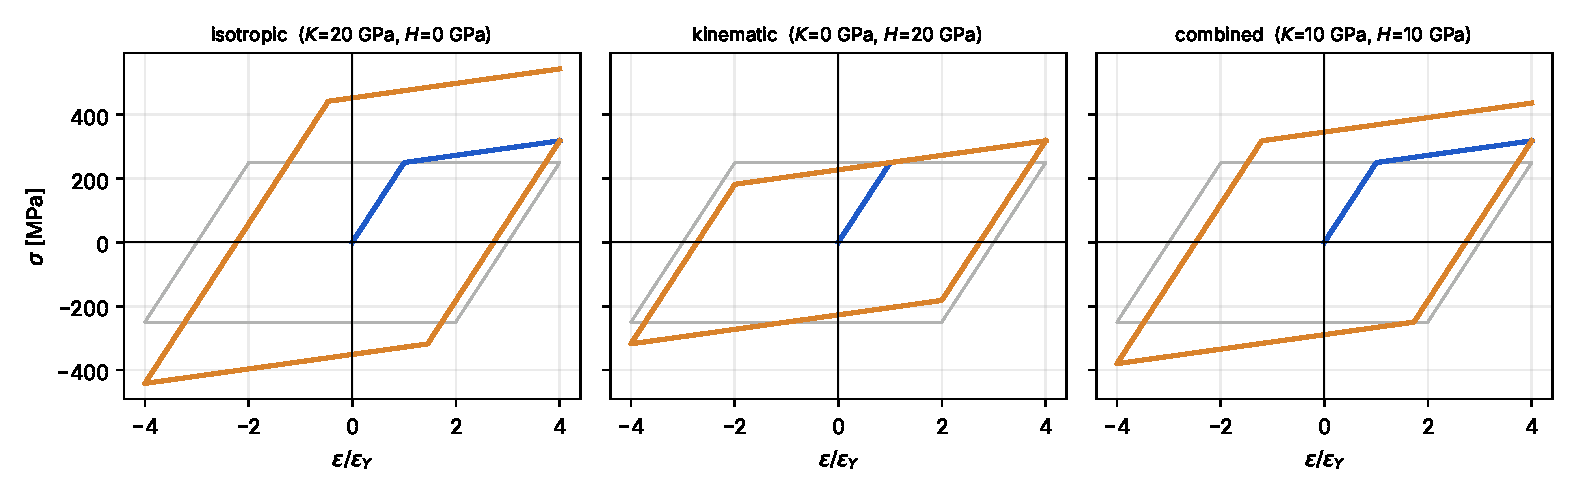
\includegraphics[width=\textwidth]{figures/ch4/filament_cycles.pdf}
\caption{Response of the filament to the strain cycle
$0\to4\varepsilon_Y\to-4\varepsilon_Y\to4\varepsilon_Y$,
$\varepsilon_Y=\sY/E$, with $E=200$\,GPa, $\sY=250$\,MPa and the same
monotonic curve, $K+H=20$\,GPa (a large value, chosen for legibility). Blue:
first loading; orange: the two reversals. Isotropic hardening (left) enlarges
the elastic range at each reversal; kinematic hardening (centre) translates
it, with early reverse yielding and a closed loop; combined hardening (right)
does both. The thin grey line is the perfectly plastic response.}
\label{fig:pl-cycles}
\end{figure}

\subsection{Energy and dissipation}\label{ssec:pl-1d-energy}
\index{dissipation!plastic}\index{energy!stored}%
The work supplied to the filament per unit volume, $\sigma\dot\varepsilon$, is
split into a stored part and a dissipated part. In the combined model, the
stored (free) energy is the elastic energy of the spring plus the energy of
two hardening springs,
\begin{equation}\label{eq:pl-1d-psi}
  \psi=\tfrac12E(\varepsilon-\varepsilon^p)^2+\tfrac12K\alpha^2+\tfrac12H\xi^2,
  \qquad \xi=\varepsilon^p\ \text{(kinematic variable)},\quad q=H\xi .
\end{equation}
Then $\dot\psi=\sigma(\dot\varepsilon-\dot\varepsilon^p)+K\alpha\dot\alpha+q\dot\varepsilon^p$
and the dissipation is
\begin{equation}\label{eq:pl-1d-diss}
  \mathcal D=\sigma\dot\varepsilon-\dot\psi=(\sigma-q)\dot\varepsilon^p-K\alpha\dot\alpha
  =\gamma\bigl(|\sigma-q|-K\alpha\bigr)=\sY\,\gamma=\sY\,\dot\alpha\ \ge0 ,
\end{equation}
where $|\sigma-q|=\sY+K\alpha$ was used, since $\gamma\ne0$ only on the yield
surface. The dissipation is the work of the friction element: its threshold
times its slip rate. The hardening springs store energy. This energy is given
back when the plastic strain is reversed in kinematic hardening; in isotropic
hardening it is never given back by the model (in metals it is the energy
stored in the dislocation structure).

\paragraph{Maximum dissipation in one dimension.}
\index{maximum plastic dissipation!one-dimensional}%
The flow rule of the perfectly plastic filament has a variational
characterization, which is the seed of Section~\ref{sec:pl-maxdiss}.
\begin{proposition}\label{prop:pl-1d-maxdiss}
Let $\Esig=[-\sY,\sY]$ and $\sigma\in\Esig$. The flow
rule~\eqref{eq:pl-1d-flow}--\eqref{eq:pl-1d-kt} holds if and only if
\[
  \sigma\,\dot\varepsilon^p\ \ge\ \sigma^\ast\,\dot\varepsilon^p\qquad\text{for all }\sigma^\ast\in\Esig .
\]
Among all admissible stresses, the actual stress maximizes the dissipated
power $\sigma^\ast\dot\varepsilon^p$, and the maximum is
$\sY|\dot\varepsilon^p|$.
\end{proposition}
\begin{proof}
If $|\sigma|<\sY$, the linear function $\sigma^\ast\mapsto\sigma^\ast\dot\varepsilon^p$ is
maximal at an interior point only if $\dot\varepsilon^p=0$; conversely the
flow rule gives $\gamma=0$. If $\sigma=\pm\sY$, the function is maximal on
$[-\sY,\sY]$ at $\pm\sY$ if and only if $\pm\dot\varepsilon^p\ge0$, that is
$\dot\varepsilon^p=\gamma\sign\sigma$ with $\gamma\ge0$.
\end{proof}

\subsection{The viscoplastic filament}\label{ssec:pl-vp1d}
\index{viscoplasticity!Perzyna}\index{viscoplasticity!filament}%
In viscoplasticity the stress may leave the elastic domain, and the plastic
strain rate depends on the distance to it, the \emph{overstress}. In the model
of Perzyna~\cite{Perzyna1966}, a dashpot of viscosity $\eta$ is placed in
parallel with the friction element, and the multiplier is given explicitly
instead of by the Kuhn--Tucker conditions:
\begin{equation}\label{eq:pl-perzyna1d}
  \sigma=E(\varepsilon-\varepsilon^{vp}),\qquad
  \dot\varepsilon^{vp}=\gamma\,\sign(\sigma),\qquad
  \gamma=\frac{\mac{f(\sigma)}}{\eta}=\frac{\mac{|\sigma|-\sY}}{\eta}.
\end{equation}
With the relaxation time $\tau=\eta/E$, and in a stress state outside the
elastic domain ($\sigma>\sY$, say), the evolution reads
\begin{equation}\label{eq:pl-perzyna-ode}
  \dot\sigma+\frac1\tau\,(\sigma-\sY)=E\dot\varepsilon .
\end{equation}
This is a linear ordinary differential equation, to which the standard
integration methods apply. In a relaxation test (strain held at
$\varepsilon_0>\sY/E$ from $t=0$), its solution is
\begin{equation}\label{eq:pl-relax}
  \sigma(t)=\sY+(E\varepsilon_0-\sY)\,e^{-t/\tau}\ \longrightarrow\ \sY\quad(t\to\infty).
\end{equation}
The stress relaxes to the yield surface. With $P\sigma=\sY\sign(\sigma)$ the
projection of $\sigma$ onto $\Esig$ when $|\sigma|>\sY$, the flow rule can be
written
\begin{equation}\label{eq:pl-dl1d}
  \dot\varepsilon^{vp}=\frac{1}{\tau E}\,(\sigma-P\sigma),
\end{equation}
which is the form of Duvaut and Lions~\cite{DuvautLions1972}. As
$\eta\to0$ the overstress vanishes and the rate-independent model is
recovered: viscoplasticity is a regularization (a penalty) of
plasticity~\cite[Sec.~1.6]{SimoHughes1998}.

%======================================================================
\section{Three-dimensional plasticity}\label{sec:pl-3d}
\index{plasticity!three-dimensional}%
The filament model extends to a three-dimensional body in small strains with
the same four ingredients. Stresses and strains are now symmetric
second-order tensors, elements of the space $\Sym$, and the plastic strain
$\epsp$ is a symmetric tensor field.

\subsection{Elastic law}\label{ssec:pl-elastic}
\index{plastic strain}\index{strain!additive decomposition}%
The strain is split additively, $\eps=\epse+\epsp$, and the stress is given by
the elastic law of Chapter~\ref{ch:elliptic} applied to the elastic part:
\begin{equation}\label{eq:pl-elastic}
  \sig=\bbC:(\eps-\epsp),\qquad
  \bbC=\kappa\,\tI\otimes\tI+2\mu\,\bbIdev\quad\text{(isotropy)},
\end{equation}
with the bulk modulus $\kappa$, the shear modulus $\mu$, and
$\bbIdev=\bbI-\tfrac13\tI\otimes\tI$ the projector onto deviatoric tensors.
For a given field $\epsp$, the plastic strain enters the equations exactly as
the thermal strain $\talpha\,\theta^D$ of Section~\ref{sec:el-energy}: it is an
\emph{initial strain} (an eigenstrain). The difference is that $\epsp$ is not
prescribed: it is an unknown, governed by an evolution law.

\subsection{Elastic domain and yield criteria}\label{ssec:pl-criteria}
\index{yield criterion}\index{elastic domain}\index{yield function}%
The elastic domain is a set of stresses and stress-like hardening variables
$\vq\in\R^m$, defined by a yield function:
\begin{equation}\label{eq:pl-domain}
  \Esig=\bigl\{(\sig,\vq)\in\Sym\times\R^m\ :\ f(\sig,\vq)\le0\bigr\}.
\end{equation}
Its interior $\{f<0\}$ is the set of elastic states, its boundary $\{f=0\}$
the yield surface. Outside $\Esig$ there are no admissible states. The
hardening variables $\vq$ describe the position and the size of the domain;
we first consider fixed $\vq$ and write $f(\sig)$.

\paragraph{Isotropy and invariants.}
\index{stress!invariants}\index{stress!deviator}\index{Haigh--Westergaard space}%
For an isotropic material, $f(\sig)$ depends only on the principal stresses
$\sigma_1,\sigma_2,\sigma_3$, symmetrically. It is convenient to split the
stress into its mean (hydrostatic) part and its deviator,
\[
  \sig=p\,\tI+\tens{s},\qquad p=\tfrac13\tr\sig,\qquad
  \tens{s}=\dev\sig=\sig-\tfrac13(\tr\sig)\,\tI,
\]
and to use the invariants $p$, $J_2=\tfrac12\tens{s}:\tens{s}$ and
$J_3=\det\tens{s}$. In the space of principal stresses, the hydrostatic axis
$\sigma_1=\sigma_2=\sigma_3$ carries $p$, and the plane orthogonal to it
through the origin (the \emph{deviatoric} or $\pi$-plane) carries $\tens{s}$.
In the $\pi$-plane, the deviator has polar coordinates $(\norm{\tens{s}},\theta)$,
where $\norm{\tens{s}}=\sqrt{\tens{s}:\tens{s}}=\sqrt{2J_2}$ and the Lode
angle $\theta$ is a function of $J_3/J_2^{3/2}$.

\paragraph{Metals are insensitive to pressure.} Plastic flow in metals is
produced by slip on crystallographic planes, driven by shear stresses. A
superposed hydrostatic pressure does not change the yield stress, and the
plastic strain is isochoric, $\tr\epsp=0$. The yield function then depends
on the deviator only, and the yield surface is a cylinder parallel to the
hydrostatic axis, described by its section in the $\pi$-plane
(Figure~\ref{fig:pl-loci}).

\begin{gbox}{Von Mises and Tresca criteria}
\index{von Mises criterion}\index{Tresca criterion}\index{equivalent stress}%
\begin{itemize}
  \item \emph{von Mises}: the elastic energy of distortion is bounded,
  \begin{equation}\label{eq:pl-mises}
    f(\sig)=\norm{\dev\sig}-\sqrt{\tfrac23}\,\sY\le0
    \quad\Longleftrightarrow\quad
    \sigma_{eq}=\sqrt{\tfrac32\,\dev\sig:\dev\sig}\le\sY .
  \end{equation}
  \item \emph{Tresca}: the maximal shear stress is bounded,
  \begin{equation}\label{eq:pl-tresca}
    f(\sig)=\max_{i,j}|\sigma_i-\sigma_j|-\sY\le0 .
  \end{equation}
\end{itemize}
Both are calibrated on the uniaxial tensile test: $\sig=\sigma\,\ve_1\otimes\ve_1$
yields at $|\sigma|=\sY$. In the $\pi$-plane the von Mises section is a circle
of radius $\sqrt{2/3}\,\sY$, and the Tresca section the regular hexagon
inscribed in it.
\end{gbox}

The two criteria differ most in shear. In tension--torsion,
$\sig=\sigma(\ve_1\otimes\ve_1)+\tau(\ve_1\otimes\ve_2+\ve_2\otimes\ve_1)$, they read
\begin{equation}\label{eq:pl-tt}
  \text{von Mises: }\ \sigma^2+3\tau^2\le\sY^2,\qquad
  \text{Tresca: }\ \sigma^2+4\tau^2\le\sY^2 ,
\end{equation}
so that the shear yield stress is $\sY/\sqrt3\approx0.577\,\sY$ for von Mises
and $\sY/2$ for Tresca. Tension--torsion experiments on most metals fall
between the two curves, closer to von Mises~\cite{Lubliner1990}.

\begin{figure}[h]
\centering
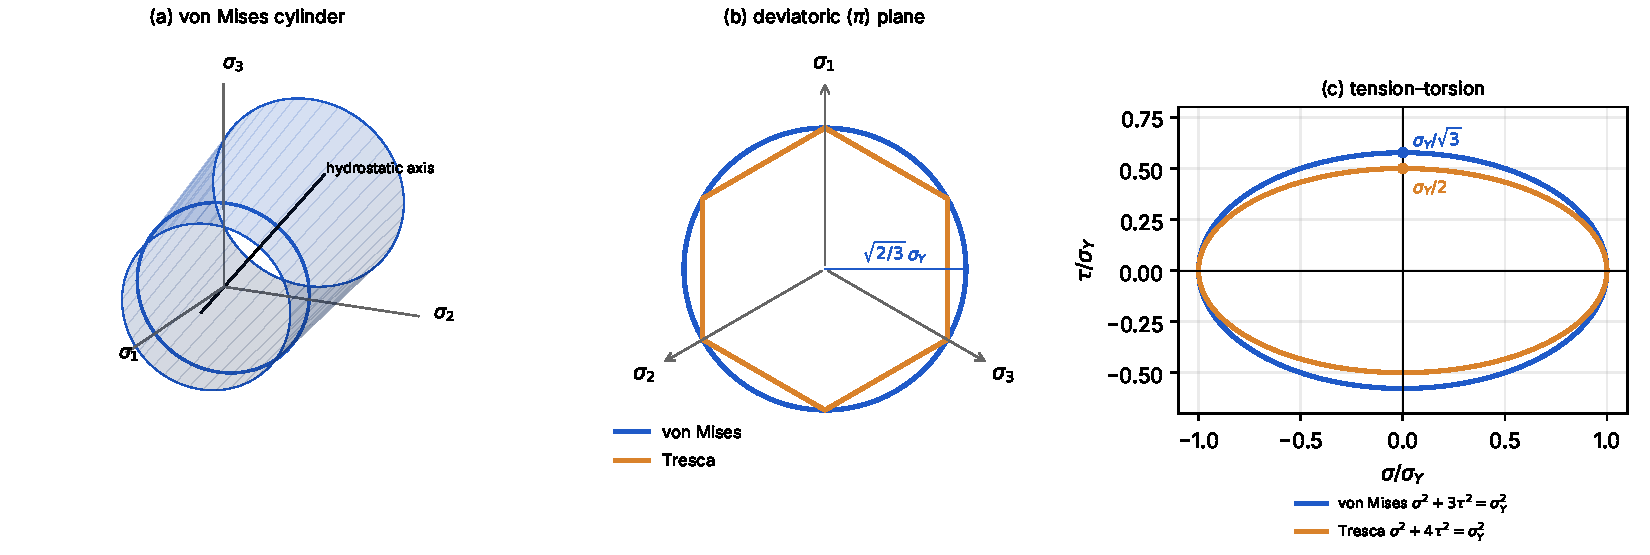
\includegraphics[width=\textwidth]{figures/ch4/yield_loci.pdf}
\caption{Left: sections of the von Mises cylinder (circle) and of the Tresca
prism (hexagon) by the $\pi$-plane; the projections of the principal axes are
drawn at $120^\circ$. Right: the same criteria in the tension--torsion plane
$(\sigma,\tau)$, ellipses~\eqref{eq:pl-tt}; the two coincide in pure tension
and differ most in pure shear.}
\label{fig:pl-loci}
\end{figure}

\paragraph{Pressure-sensitive materials.}
\index{Drucker--Prager criterion}\index{Mohr--Coulomb criterion}%
Soils, concrete, rocks and polymers are sensitive to pressure: confinement
raises their strength. The \emph{Drucker--Prager} criterion
$f(\sig)=\sigma_{eq}+\alpha_{DP}\tr\sig-\sigma_0\le0$ is a cone around the
hydrostatic axis, and the \emph{Mohr--Coulomb} criterion
$f(\sig)=(\sigma_1-\sigma_3)+(\sigma_1+\sigma_3)\sin\phi-2c\cos\phi\le0$
($\sigma_1\ge\sigma_2\ge\sigma_3$, friction angle $\phi$, cohesion $c$) a
hexagonal pyramid~\cite{Salencon2002}. All the criteria above define convex
sets; Section~\ref{sec:pl-maxdiss} explains why convexity is not an accident.

\subsection{Flow rule, hardening rule and loading conditions}\label{ssec:pl-flow}
\index{flow rule}\index{hardening rule}\index{flow rule!associative}%
The general model of rate-independent plasticity~\cite[Sec.~2.2]{SimoHughes1998}
gives the rates of the plastic strain and of the hardening variables in terms
of a single multiplier $\gamma$.
\begin{gbox}{Rate-independent plasticity}
\begin{align}
  &\sig=\bbC:(\eps-\epsp) && \text{elastic law},\label{eq:pl-box-el}\\
  &\Esig=\{(\sig,\vq)\ :\ f(\sig,\vq)\le0\} && \text{elastic domain},\label{eq:pl-box-dom}\\
  &\dot\eps^p=\gamma\,\tens{r}(\sig,\vq),\qquad \dot\vq=-\gamma\,\bbD\,\vect{h}(\sig,\vq)
  && \text{flow and hardening rules},\label{eq:pl-box-flow}\\
  &\gamma\ge0,\quad f(\sig,\vq)\le0,\quad\gamma\,f(\sig,\vq)=0 && \text{Kuhn--Tucker conditions},\label{eq:pl-box-kt}\\
  &\gamma\,\dot f(\sig,\vq)=0 && \text{consistency condition}.\label{eq:pl-box-cons}
\end{align}
The flow is \emph{associative} when the directions are the gradients of the
yield function: $\tens r=\partial_{\sig}f$, $\vect h=\partial_{\vq}f$.
\end{gbox}
\noindent Here $\bbD$ is a symmetric positive definite matrix of
\emph{hardening moduli} (generalized plastic moduli). In the associative case
the plastic strain rate is normal to the yield surface: this is the
\emph{normality rule}. The four cases of loading and unloading of the
filament hold without change, because they rest only on the following
property.

\begin{lemma}[Persistency]\label{lem:pl-persist}
For a piecewise smooth process with $f(\sig(t),\vq(t))\le0$ for all $t$, the
condition $f(t)=0$ implies $\dot f(t)\le0$, where $\dot f$ is the right time
derivative.
\end{lemma}
\begin{proof}
For $\Delta t>0$, $f(t+\Delta t)\le0=f(t)$. Dividing by $\Delta t$ and letting
$\Delta t\to0$ gives $\dot f(t)\le0$.
\end{proof}

\subsection{The plastic multiplier and the continuum tangent}\label{ssec:pl-tangent}
\index{plastic multiplier}\index{tangent modulus!continuum elastoplastic}%
Let the state be on the yield surface, $f(\sig,\vq)=0$, and the strain rate
$\dot\eps$ be given. Write $\partial_{\sig}f$ and $\partial_{\vq}f$ for the
gradients at the current state. By the chain rule and~\eqref{eq:pl-box-flow},
\begin{equation}\label{eq:pl-fdot}
  \dot f=\partial_{\sig}f:\dot\sig+\partial_{\vq}f\cdot\dot\vq
  =\partial_{\sig}f:\bbC:\dot\eps
  -\gamma\,\bigl(\partial_{\sig}f:\bbC:\tens r+\partial_{\vq}f\cdot\bbD\,\vect h\bigr).
\end{equation}
\begin{proposition}[Plastic multiplier and continuum tangent]\label{prop:pl-cep}
Assume that the \emph{hardening modulus}
$h_p=\partial_{\sig}f:\bbC:\tens r+\partial_{\vq}f\cdot\bbD\,\vect h$ is
positive. Then the Kuhn--Tucker and consistency conditions determine
\begin{equation}\label{eq:pl-gamma}
  \gamma=\frac{\mac{\partial_{\sig}f:\bbC:\dot\eps}}{h_p},
\end{equation}
and the stress rate is $\dot\sig=\bbC:\dot\eps$ if $\gamma=0$, and
$\dot\sig=\bbCep:\dot\eps$ if $\gamma>0$, with
\begin{equation}\label{eq:pl-cep}
  \bbCep=\bbC-\frac{(\bbC:\tens r)\otimes(\bbC:\partial_{\sig}f)}{h_p}.
\end{equation}
The continuum tangent $\bbCep$ is symmetric if the flow is associative.
\end{proposition}
\begin{proof}
If $\partial_{\sig}f:\bbC:\dot\eps<0$, then by~\eqref{eq:pl-fdot}
$\dot f<0$ for every $\gamma\ge0$, and consistency gives $\gamma=0$. If
$\partial_{\sig}f:\bbC:\dot\eps>0$, then $\gamma=0$ would give $\dot f>0$,
which Lemma~\ref{lem:pl-persist} excludes; hence $\gamma>0$, $\dot f=0$, and
$\gamma=\partial_{\sig}f:\bbC:\dot\eps/h_p$. The neutral case gives
$\gamma=0$. Then
$\dot\sig=\bbC:(\dot\eps-\gamma\,\tens r)=\bbC:\dot\eps-(\bbC:\tens r)\,
(\bbC:\partial_{\sig}f:\dot\eps)/h_p$, using the major symmetry of $\bbC$.
If $\tens r=\partial_{\sig}f$ the two vectors of the dyad coincide.
\end{proof}
The quantity $\partial_{\sig}f:\bbC:\dot\eps$ is the rate of $f$ produced by a
purely elastic response, $\dot f^\trial$, with the trial stress rate
$\dot\sig^\trial=\bbC:\dot\eps$. Geometrically, the material loads plastically
when $\dot\sig^\trial$ points out of the elastic domain, and unloads when it
points inwards (Figure~\ref{fig:pl-loading}). The loading criterion
$\dot f^\trial>0$ is written in terms of the strain rate, which is the
quantity controlled in a finite element computation.

\begin{figure}[h]
\centering
\begin{tikzpicture}[scale=1.0,>=Latex]
  \fill[cu!10,rotate=30] (0,0) ellipse (2.4 and 1.4);
  \draw[thick,cu,rotate=30] (0,0) ellipse (2.4 and 1.4);
  \node[cu] at (-0.6,0.0) {$\Esig\ (f<0)$};
  \node[cu] at (-1.6,2.3) {$\partial\Esig\ (f=0)$};
  \node[gray] at (3.9,-1.6) {$f>0$: not admissible};
  % boundary point: ellipse x=2.4cos t, y=1.4 sin t, t=-35deg, rotated 30
  \coordinate (P) at ({2.4*cos(-35)*cos(30)-1.4*sin(-35)*sin(30)},{2.4*cos(-35)*sin(30)+1.4*sin(-35)*cos(30)});
  % outward normal direction ~ (cos t/2.4, sin t/1.4) rotated
  \coordinate (N) at ($(P)+({0.83*(cos(-35)/2.4*cos(30)-sin(-35)/1.4*sin(30))*2.2},{0.83*(cos(-35)/2.4*sin(30)+sin(-35)/1.4*cos(30))*2.2})$);
  \draw[->,very thick] (P) -- (N) node[below right] {$\partial_{\sig}f$};
  % tangent line
  \draw[dashed,gray] ($(P)!2.2cm!90:(N)$) -- ($(P)!-2.0cm!90:(N)$);
  \draw[->,very thick,orange!80!black] (P) -- ++(1.6,0.9) node[right] {$\dot\sig^\trial=\bbC:\dot\eps$\ \ (loading)};
  \draw[->,very thick,cphi] (P) -- ++(-1.0,0.75) node[above left] {unloading};
  \fill (P) circle (1.6pt) node[left] {$(\sig,\vq)\ $};
\end{tikzpicture}
\caption{Loading and unloading, after Simo and
Hughes~\cite[Fig.~2-4]{SimoHughes1998}. At a point of the yield surface the
material loads plastically if the trial stress rate $\bbC:\dot\eps$ points to
the outside of the tangent plane (dashed), $\partial_{\sig}f:\bbC:\dot\eps>0$,
and unloads elastically if it points to the inside.}
\label{fig:pl-loading}
\end{figure}
The criterion $\dot f^\trial>0$ stays valid for softening materials, as long as $h_p>0$, whereas a criterion on the stress
rate would not. For a non-associative flow ($\tens r\ne\partial_{\sig}f$, as
for many soils), $\bbCep$ is not symmetric, and the tangent stiffness matrix
of a finite element computation is not symmetric either.

\subsection{\texorpdfstring{$J_2$}{J2} flow theory}\label{ssec:pl-j2}
\index{J2 flow theory@$J_2$ flow theory}\index{von Mises criterion!with hardening}\index{equivalent plastic strain}%
The model most used for metals combines the von Mises criterion with
isotropic and kinematic hardening and the associative flow
rule~\cite[Sec.~2.3.2]{SimoHughes1998}. Let $\tbeta$ be the back stress, a
deviatoric tensor (the centre of the von Mises cylinder), and $\alpha$ the
equivalent plastic strain. With the relative stress $\teta=\dev\sig-\tbeta$
and the unit normal $\tn=\teta/\norm{\teta}$,
\begin{gbox}{$J_2$ plasticity with linear isotropic and kinematic hardening}
\begin{align}
  &f(\sig,\tbeta,\alpha)=\norm{\dev\sig-\tbeta}-\sqrt{\tfrac23}\,(\sY+K\alpha),\label{eq:pl-j2-f}\\
  &\dot\eps^p=\gamma\,\tn,\qquad
  \dot{\tbeta}=\tfrac23H\,\gamma\,\tn,\qquad
  \dot\alpha=\sqrt{\tfrac23}\,\gamma ,\label{eq:pl-j2-flow}\\
  &\gamma=\frac{\mac{\tn:\dot\eps}}{1+\dfrac{K+H}{3\mu}},\qquad
  \bbCep=\kappa\,\tI\otimes\tI+2\mu\Bigl[\bbIdev-\frac{\tn\otimes\tn}{1+\dfrac{K+H}{3\mu}}\Bigr]
  \quad(\gamma>0).\label{eq:pl-j2-cep}
\end{align}
\end{gbox}
\noindent The plastic strain rate is deviatoric (isochoric flow), and
$\dot\alpha=\sqrt{2/3}\,\norm{\dot\eps^p}$. The factor $\sqrt{2/3}$ makes $\alpha$
equal to $|\varepsilon^p_{11}|$ in uniaxial tension, where
$\dot\eps^p=\dot\varepsilon^p_{11}\,\diag(1,-\tfrac12,-\tfrac12)$. To derive
the multiplier, note that $\tn$ is deviatoric and unitary, so that
$\tn:\dev\dot\sig=2\mu\,\tn:(\dot\eps-\gamma\tn)=2\mu\,\tn:\dot\eps-2\mu\gamma$, and
\[
  \dot f=\tn:(\dev\dot\sig-\dot{\tbeta})-\sqrt{\tfrac23}K\dot\alpha
  =2\mu\,\tn:\dot\eps-\gamma\bigl(2\mu+\tfrac23H+\tfrac23K\bigr).
\]
This is~\eqref{eq:pl-gamma} with $h_p=2\mu+\tfrac23(K+H)$; the tangent follows
from~\eqref{eq:pl-cep} with $\bbC:\tn=2\mu\tn$. For perfect plasticity
($K=H=0$), $\bbCep=\kappa\,\tI\otimes\tI+2\mu(\bbIdev-\tn\otimes\tn)$: the
stiffness in the direction $\tn$ vanishes.

In uniaxial stress the model reduces to the filament of
Section~\ref{ssec:pl-1d-kin}, with the same $K$ and $H$ and the back stress
$q=\tfrac32\beta_{11}=H\varepsilon^p_{11}$ (Exercise~\ref{exo:pl-uniaxial}).
In three dimensions, Simo and Hughes reserve the letter $\vq$ for the vector of
all stress-like hardening variables; for $J_2$ plasticity
$\vq=(-K\alpha,\,-\tbeta)$, $\bbD=\diag(K,\tfrac23H\,\bbI)$, and
\[
  f(\sig,\vq)=\norm{\dev\sig+\vq_{\mathrm{kin}}}-\sqrt{\tfrac23}\,(\sY-q_{\mathrm{iso}}),
\]
so that the associative rules $\dot\vq=-\gamma\,\bbD\,\partial_{\vq}f$
of~\eqref{eq:pl-box-flow} give back~\eqref{eq:pl-j2-flow}.

In the space of stresses, isotropic hardening expands the von Mises cylinder
and kinematic hardening translates it along the direction of plastic flow
(Figure~\ref{fig:pl-hardening}). Measured yield surfaces of metals after
plastic loading show both effects, with a translation that dominates at small
offsets~\cite{Lubliner1990}.

\begin{figure}[h]
\centering
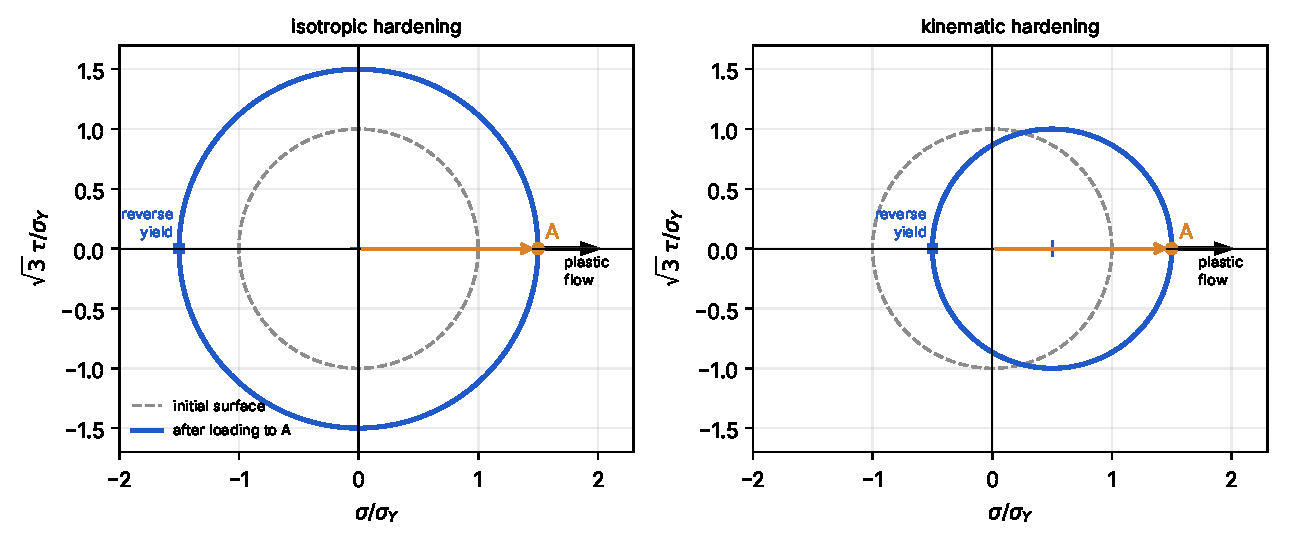
\includegraphics[width=0.85\textwidth]{figures/ch4/hardening_surfaces.pdf}
\caption{Section of the von Mises surface by the tension--torsion plane
$(\sigma,\sqrt3\tau)$, before (dashed) and after a tensile loading up to
$A=1.5\,\sY$. Isotropic hardening (left) expands the surface around the
origin; kinematic hardening (right) translates it, and reverse yielding in
compression starts at $\sigma=-0.5\,\sY$ instead of $-1.5\,\sY$
(Bauschinger effect). The plastic strain rate at $A$ is normal to the
surface.}
\label{fig:pl-hardening}
\end{figure}

\paragraph{Nonlinear hardening.}
\index{hardening!nonlinear}\index{Armstrong--Frederick model}\index{Voce law}%
Linear hardening is an approximation. Saturating laws are more realistic: the
\emph{Voce} law replaces $\sY+K\alpha$ by
$R(\alpha)=\sigma_\infty-(\sigma_\infty-\sY)e^{-\delta\alpha}$, and the
\emph{Armstrong--Frederick} law~\cite{ArmstrongFrederick1966} adds a recall
term to the kinematic rule, $\dot{\tbeta}=\tfrac23H\dot\eps^p-\zeta\,\tbeta\,\dot\alpha$,
which bounds the back stress. Formulas~\eqref{eq:pl-j2-cep} hold with $K$
replaced by $R'(\alpha)$ and $H$ by an effective modulus. The
Armstrong--Frederick law is not associative: the flow derives from a
pseudo-potential $F\ne f$~\cite{LemaitreChaboche1990}. It is therefore not a
generalized standard material in the sense of Section~\ref{sec:pl-gsm}, and
the results of Section~\ref{sec:pl-maxdiss} do not apply to it, although its
dissipation is non-negative (Exercise~\ref{exo:pl-af}).

\paragraph{Corners.}
\index{Tresca criterion!flow rule}\index{yield surface!corner}%
The Tresca criterion is not differentiable on the edges of the hexagon. It is
the intersection of six smooth (planar) criteria $f_\beta\le0$, and the flow
rule is then written with one multiplier per active surface,
$\dot\eps^p=\sum_\beta\gamma_\beta\,\partial_{\sig}f_\beta$ with
$\gamma_\beta\ge0$, $f_\beta\le0$, $\gamma_\beta f_\beta=0$ (Koiter's
rule~\cite{Koiter1953}). At a corner the flow direction can be any
combination of the normals of the adjacent faces: it lies in the cone of
normals. Section~\ref{sec:pl-maxdiss} gives this rule a single expression.

%======================================================================
\section{Thermodynamics and generalized standard materials}\label{sec:pl-gsm}
\index{generalized standard material}\index{thermodynamics!of plasticity}%
The model of Section~\ref{sec:pl-3d} was written as a list of rules. Halphen
and Nguyen~\cite{HalphenNguyen1975} showed that, for a large class of
materials, these rules follow from two convex functions: a free energy, which
gives the state laws, and a dissipation potential, which gives the evolution
laws. This structure, the one of \emph{generalized standard materials}
(GSM), guarantees the second principle of thermodynamics and is the source of
the variational principles and of the convergence properties used in this
chapter and the next two~\cite{GermainNguyenSuquet1983,LemaitreChaboche1990,Nguyen2000}.
We follow the presentation of Kondo and Maitournam~\cite{KondoMaitournam2023},
in the isothermal setting and in the notation of Simo and Hughes. The recipe
has three steps: choose the state variables; choose a free energy, which gives
the reversible part of the forces (the \emph{state laws}); choose a
dissipation potential, which gives their irreversible part (the
\emph{evolution laws}).

\subsection{State variables, state laws and dissipation}\label{ssec:pl-state}
\index{state laws}\index{free energy}\index{internal variables}\index{thermodynamic forces}%
The state of a material point is described by the total strain $\eps$ and by
internal variables $\vz=(\epsp,\valpha)$: the plastic strain and strain-like
hardening variables $\valpha\in\R^m$. The (Helmholtz) free energy per unit
volume, at fixed temperature, is
\begin{equation}\label{eq:pl-psi}
  \psi(\eps,\epsp,\valpha)=\tfrac12(\eps-\epsp):\bbC:(\eps-\epsp)+\psi_h(\valpha),
  \qquad\text{linear hardening: }\ \psi_h(\valpha)=\tfrac12\,\valpha\cdot\bbD\,\valpha .
\end{equation}
The \emph{state laws} define the stress and the \emph{thermodynamic forces}
conjugate to the internal variables:
\begin{equation}\label{eq:pl-statelaws}
  \sig=\frac{\partial\psi}{\partial\eps}=-\frac{\partial\psi}{\partial\epsp},
  \qquad
  \vq=-\frac{\partial\psi}{\partial\valpha}=-\bbD\,\valpha,
  \qquad
  \vSig:=-\frac{\partial\psi}{\partial\vz}=(\sig,\vq).
\end{equation}
The \emph{generalized stress} $\vSig$ collects the forces, and the
\emph{generalized plastic strain rate} $\dot\vz$ the fluxes, with the pairing
$\vSig\cdot\dot\vz=\sig:\dot\eps^p+\vq\cdot\dot\valpha$.

\paragraph{Clausius--Duhem inequality.}
\index{Clausius--Duhem inequality}\index{dissipation}%
In an isothermal process, the second principle requires that the intrinsic
dissipation, the power supplied minus the rate of free energy, be
non-negative. With the state laws,
\begin{equation}\label{eq:pl-CD}
  \mathcal D=\sig:\dot\eps-\dot\psi
  =\sig:\dot\eps-\frac{\partial\psi}{\partial\eps}:\dot\eps-\frac{\partial\psi}{\partial\vz}\cdot\dot\vz
  =\vSig\cdot\dot\vz=\sig:\dot\eps^p+\vq\cdot\dot\valpha\ \ge0 .
\end{equation}
The total strain is not a dissipative variable: the whole stress is
reversible, $\sig=\partial\psi/\partial\eps$, and the dissipation comes only
from the internal variables~\cite{KondoMaitournam2023}. (In a Kelvin--Voigt
viscoelastic solid, by contrast, the stress has an irreversible part.)
The dissipation is a product of forces and fluxes. In the language of Simo and
Hughes, the hardening rule $\dot\vq=-\gamma\bbD\,\partial_{\vq}f$ is the same as
$\dot\valpha=\gamma\,\partial_{\vq}f$, by~\eqref{eq:pl-statelaws}. The
associative model~\eqref{eq:pl-box-flow} therefore reads, in the generalized
variables,
\begin{equation}\label{eq:pl-assoc-gen}
  \dot\vz=\gamma\,\partial_{\vSig}f(\vSig),\qquad
  \gamma\ge0,\quad f(\vSig)\le0,\quad\gamma f(\vSig)=0 :
\end{equation}
the generalized plastic strain rate is normal to the elastic domain $\Esig$ in
the space of generalized stresses.

\paragraph{Example: $J_2$ plasticity.} The model~\eqref{eq:pl-j2-f}--\eqref{eq:pl-j2-flow}
has the internal variables $\valpha=(\alpha,\valpha_{\mathrm{kin}})$ with
$\valpha_{\mathrm{kin}}=\epsp$ (the kinematic variable follows the plastic
strain), the hardening energy and forces
\[
  \psi_h=\tfrac12K\alpha^2+\tfrac13H\,\epsp:\epsp,\qquad
  q_{\mathrm{iso}}=-K\alpha,\qquad \vq_{\mathrm{kin}}=-\tfrac23H\,\epsp=-\tbeta ,
\]
and the dissipation, computed as in~\eqref{eq:pl-1d-diss},
\begin{equation}\label{eq:pl-j2-diss}
  \mathcal D=\gamma\bigl(\tn:(\dev\sig-\tbeta)-\sqrt{\tfrac23}K\alpha\bigr)
  =\gamma\sqrt{\tfrac23}\,\bigl(\sY+K\alpha-K\alpha\bigr)=\sY\,\dot\alpha .
\end{equation}
As for the filament, only the initial yield stress dissipates; the hardening
part of the plastic work is stored.

\subsection{Generalized standard materials}\label{ssec:pl-gsm-def}
\index{dissipation potential}\index{generalized standard material!definition}\index{normality rule}%
\begin{definition}[Halphen--Nguyen~\cite{HalphenNguyen1975}]\label{def:pl-gsm}
A material is \emph{generalized standard} if its state laws derive from a free
energy $\psi(\eps,\vz)$, convex in $(\eps,\vz)$, and if there is a
\emph{dissipation potential} $\varphi(\dot\vz)$, convex, lower
semicontinuous, with $\varphi\ge0$ and $\varphi(\vzero)=0$, such that
\begin{equation}\label{eq:pl-normality}
  \vSig\in\partial\varphi(\dot\vz)
  \qquad\Longleftrightarrow\qquad
  \dot\vz\in\partial\varphi^\ast(\vSig).
\end{equation}
\end{definition}
\noindent The subdifferential $\partial\varphi$ is the set of slopes of the
supporting hyperplanes of $\varphi$ (it reduces to the gradient where
$\varphi$ is differentiable), and $\varphi^\ast$ is the Legendre--Fenchel
transform of $\varphi$ (Section~\ref{sec:var-dual}), the \emph{dual
dissipation potential}. The equivalence of the two forms
of~\eqref{eq:pl-normality} is the equality case of the Fenchel--Young
inequality. The first form, written as
$\vzero\in\partial_{\vz}\psi+\partial\varphi(\dot\vz)$, is a generalized Biot
equation; the second is the \emph{normality rule}.

\begin{proposition}\label{prop:pl-gsm-CD}
A generalized standard material satisfies the Clausius--Duhem inequality:
$\mathcal D=\vSig\cdot\dot\vz\ge\varphi(\dot\vz)\ge0$.
\end{proposition}
\begin{proof}
The subgradient inequality for $\varphi$ at $\dot\vz$, tested at $\vzero$,
gives $0=\varphi(\vzero)\ge\varphi(\dot\vz)+\vSig\cdot(\vzero-\dot\vz)$.
\end{proof}
A material defined by two convex potentials is thus thermodynamically
admissible \emph{for every process}: the second principle is built into the
structure. The modeller chooses $\psi$ and $\varphi$; no further check is
needed.

\paragraph{Rate independence and the elastic domain.}
\index{support function}\index{indicator function}\index{rate independence}%
Rate-independent plasticity corresponds to dissipation potentials that are
positively homogeneous of degree one: $\varphi(\lambda\dot\vz)=\lambda\,\varphi(\dot\vz)$
for $\lambda>0$.
\begin{proposition}\label{prop:pl-rateindep}
Let $\varphi\ge0$ be convex, lower semicontinuous and positively homogeneous of
degree one, and $\Esig=\partial\varphi(\vzero)=\{\vSig:\ \vSig\cdot\dot\vz\le\varphi(\dot\vz)\ \forall\dot\vz\}$.
Then $\Esig$ is closed and convex, contains $\vzero$, and
\[
  \varphi^\ast=I_{\Esig},\qquad
  \varphi(\dot\vz)=\pi_{\Esig}(\dot\vz):=\sup_{\vSig^\ast\in\Esig}\vSig^\ast\cdot\dot\vz ,
\]
where $I_{\Esig}$ is the indicator function of $\Esig$ ($0$ on $\Esig$,
$+\infty$ outside) and $\pi_{\Esig}$ its support function. Conversely,
every closed convex set containing $\vzero$ defines such a potential.
\end{proposition}
\begin{proof}
For a given $\vSig$, the function $\dot\vz\mapsto\vSig\cdot\dot\vz-\varphi(\dot\vz)$
is positively homogeneous. Either it is $\le0$ everywhere, and its supremum
$\varphi^\ast(\vSig)$ is $0$ (value at $\dot\vz=\vzero$); or it is positive
somewhere, and then $\varphi^\ast(\vSig)=+\infty$ by scaling. Hence
$\varphi^\ast=I_{\Esig}$ with $\Esig$ as stated. As $\varphi$ is convex and
lower semicontinuous, $\varphi=\varphi^{\ast\ast}=I_{\Esig}^\ast=\pi_{\Esig}$.
\end{proof}
The dual potential of a rate-independent material is the indicator of its
elastic domain, and the normality rule~\eqref{eq:pl-normality} becomes
$\dot\vz\in\partial I_{\Esig}(\vSig)$. Since $\partial\varphi(\lambda\dot\vz)=\partial\varphi(\dot\vz)$
for $\lambda>0$, a change of time scale leaves the evolution unchanged: this
is rate independence. The dissipation potential is the \emph{dissipation
function} $\pi_{\Esig}$: by Proposition~\ref{prop:pl-gsm-CD} and the
definition of $\Esig$, $\mathcal D=\pi_{\Esig}(\dot\vz)$ for the actual
process. For $J_2$ plasticity with isotropic hardening,
$\pi_{\Esig}(\dot\eps^p,\dot\alpha)=\sY\dot\alpha$ on the admissible rates
(Example~\ref{ex:pl-mises-pi}), in agreement
with~\eqref{eq:pl-j2-diss}.

\paragraph{Viscoplasticity.}
\index{viscoplasticity!dual potential}\index{Norton--Hoff law}\index{viscoplasticity!Duvaut--Lions}%
A smooth, finite dual potential gives a viscoplastic material. With a
viscosity $\eta$, or a reference strain rate $\dot\varepsilon_0$ and an
exponent $m$:
\begin{align}
  \text{Perzyna:}\quad&\varphi^\ast(\vSig)=\frac1{2\eta}\mac{f(\vSig)}^2,
  &&\dot\vz=\frac1\eta\,\mac{f(\vSig)}\,\partial_{\vSig}f,\label{eq:pl-perzyna}\\
  \text{Norton--Hoff:}\quad&\varphi^\ast(\sig)=\frac{\sigma_0\dot\varepsilon_0}{m+1}\,
  \Bigl\langle\frac{\sigma_{eq}-\sY}{\sigma_0}\Bigr\rangle^{m+1},
  &&\dot\eps^p=\dot\varepsilon_0\Bigl\langle\frac{\sigma_{eq}-\sY}{\sigma_0}\Bigr\rangle^{m}\,\frac32\,\frac{\dev\sig}{\sigma_{eq}} .\label{eq:pl-norton}
\end{align}
The Duvaut--Lions model~\cite{DuvautLions1972} uses the squared distance to
$\Esig$ instead, $\varphi^\ast=\tfrac{1}{2\tau}\,\mathrm{dist}_E^2(\vSig,\Esig)$,
measured in the energy norm~\eqref{eq:pl-energynorm} below, with a
relaxation time $\tau$. Its one-dimensional form is~\eqref{eq:pl-dl1d}. As
$\eta\to0$ (or $\tau\to0$) the Perzyna and Duvaut--Lions potentials tend to
$I_{\Esig}$: the rate-independent model is their limit.

\subsection{A dictionary}\label{ssec:pl-dictionary}
Simo and Hughes and the French school of Halphen, Nguyen, Germain and Suquet
describe the same model in two languages. Table~\ref{tab:pl-dictionary} gives
the correspondence used in this book.

\begin{table}[h]
\centering\small
\renewcommand{\arraystretch}{1.2}
\begin{tabular}{@{}lll@{}}
\toprule
 & \sffamily Simo--Hughes~\cite{SimoHughes1998} & \sffamily Halphen--Nguyen~\cite{HalphenNguyen1975}\\
\midrule
internal variables & $\epsp$, $\valpha$ & $\vz=(\epsp,\valpha)$\\
forces & $\sig$, $\vq=-\bbD\valpha$ & $\vSig=(\sig,\vq)=-\partial_{\vz}\psi$\\
elastic domain & $f(\sig,\vq)\le0$ & $\Esig=\partial\varphi(\vzero)$\\
flow rule & $\dot\eps^p=\gamma\,\partial_{\sig}f$, $\dot\vq=-\gamma\bbD\,\partial_{\vq}f$ & $\dot\vz\in\partial\varphi^\ast(\vSig)=\partial I_{\Esig}(\vSig)$\\
loading/unloading & Kuhn--Tucker, consistency & normal cone (Section~\ref{sec:pl-maxdiss})\\
dissipation & $\sig:\dot\eps^p+\vq\cdot\dot\valpha$ & $\varphi(\dot\vz)=\pi_{\Esig}(\dot\vz)$\\
principle & maximum plastic dissipation & normality, monotonicity\\
energy norm & $\sig:\bbS:\sig+\vq\cdot\bbD^{-1}\vq$ & same\\
\bottomrule
\end{tabular}
\caption{Simo--Hughes and generalized standard materials: one model, two
notations.}
\label{tab:pl-dictionary}
\end{table}

\paragraph{The complementary energy norm.}
\index{energy!complementary (plasticity)}%
The last line of the table defines a scalar product on generalized stresses,
\begin{equation}\label{eq:pl-energynorm}
  \scal{\vSig}{\vSig'}_{E}=\sig:\bbS:\sig'+\vq\cdot\bbD^{-1}\vq',\qquad
  \norm{\vSig}_E^2=\scal{\vSig}{\vSig}_E ,
\end{equation}
where $\tfrac12\norm{\vSig}_E^2$ is the complementary energy, elastic plus
hardening. Chapter~5 shows that the implicit integration of the
flow rule is the projection of a trial state onto $\Esig$ in this norm.

%======================================================================
\section{The principle of maximum plastic dissipation}\label{sec:pl-maxdiss}
\index{maximum plastic dissipation}%
The normality rule has a variational form, which extends
Proposition~\ref{prop:pl-1d-maxdiss}: among all admissible generalized
stresses, the actual one maximizes the dissipated power. It was postulated by
Hill~\cite{Hill1950}; it also follows from Drucker's stability
postulate~\cite{Drucker1951,Lubliner1990}. We first recall a few notions of
convex analysis~\cite{RockafellarConvex}.

\subsection{Normal cones}\label{ssec:pl-cones}
\index{normal cone}\index{subdifferential}%
Let $\mathcal K$ be a nonempty closed convex set in a space with scalar product
$\vx\cdot\vy$.
\begin{gbox}{Normal cone and support function}
\begin{itemize}
  \item The \emph{normal cone} to $\mathcal K$ at $\vx\in \mathcal K$ is the set of directions
  that make an obtuse angle with every chord from $\vx$:
  $N_{\mathcal K}(\vx)=\{\vy:\ \vy\cdot(\vx'-\vx)\le0\ \ \forall\vx'\in \mathcal K\}$. It is
  $\{\vzero\}$ at interior points, a half-line along the outward normal at a
  smooth boundary point, and a cone of normals at a corner.
  \item $N_{\mathcal K}(\vx)=\partial I_{\mathcal K}(\vx)$: the normal cone is the subdifferential
  of the indicator function.
  \item $I_{\mathcal K}^\ast=\pi_{\mathcal K}$, and by Fenchel--Young, for $\vx\in \mathcal K$:
  $\ \vy\in N_{\mathcal K}(\vx)\iff\vx\in\partial\pi_{\mathcal K}(\vy)\iff\vx\cdot\vy=\pi_{\mathcal K}(\vy)$.
  \item If $\mathcal K=\{f\le0\}$ with $f$ convex and differentiable and $f(\vx_0)<0$ for
  some $\vx_0$ (\emph{Slater condition}), then $N_{\mathcal K}(\vx)=\{\vzero\}$ if
  $f(\vx)<0$ and $N_{\mathcal K}(\vx)=\{\gamma\nabla f(\vx):\gamma\ge0\}$ if $f(\vx)=0$.
  For $\mathcal K=\bigcap_\beta\{f_\beta\le0\}$, $N_{\mathcal K}(\vx)$ is the set of combinations
  $\sum_\beta\gamma_\beta\nabla f_\beta(\vx)$ with $\gamma_\beta\ge0$ and
  $\gamma_\beta=0$ when $f_\beta(\vx)<0$.
\end{itemize}
\end{gbox}
The first three items follow from the definitions and from
Section~\ref{sec:var-dual}; the last one is proved
in~\cite[Sec.~23]{RockafellarConvex}.

\subsection{The principle and its equivalent forms}\label{ssec:pl-maxdiss-thm}
\begin{theorem}[Maximum plastic dissipation]\label{thm:pl-maxdiss}
Let $\Esig$ be closed and convex with $\vzero\in\Esig$, let $\vSig\in\Esig$ and
let $\dot\vz$ be a generalized plastic strain rate. The following are
equivalent.
\begin{enumerate}[label=(\alph*)]
  \item \emph{Maximum dissipation:} $\vSig\cdot\dot\vz\ge\vSig^\ast\cdot\dot\vz$
  for all $\vSig^\ast\in\Esig$.
  \item \emph{Normality:} $\dot\vz\in N_{\Esig}(\vSig)=\partial I_{\Esig}(\vSig)$.
  \item \emph{Generalized standard form:} $\vSig\in\partial\pi_{\Esig}(\dot\vz)$.
  \item \emph{Dissipation identity:} $\mathcal D=\vSig\cdot\dot\vz=\pi_{\Esig}(\dot\vz)$.
\end{enumerate}
If moreover $\Esig=\{f\le0\}$ with $f$ convex, differentiable and
$f(\vzero)<0$, they are equivalent to
\begin{enumerate}[label=(\alph*),start=5]
  \item \emph{associative flow rule and Kuhn--Tucker conditions:}
  $\dot\vz=\gamma\,\partial_{\vSig}f(\vSig)$, $\gamma\ge0$, $f(\vSig)\le0$,
  $\gamma f(\vSig)=0$.
\end{enumerate}
\end{theorem}
\begin{proof}
(a)$\iff$(b): (a) reads $\dot\vz\cdot(\vSig^\ast-\vSig)\le0$ for all
$\vSig^\ast\in\Esig$, the definition of the normal cone.
(b)$\iff$(c)$\iff$(d): third item of the box above, with $\mathcal K=\Esig$,
$\vx=\vSig$, $\vy=\dot\vz$.
(b)$\iff$(e): fourth item, with $\vx_0=\vzero$.
\end{proof}

\begin{figure}[h]
\centering
\begin{tikzpicture}[scale=1.05,>=Latex]
  \def\domain{(2.4,0) -- (1.6,1.5) .. controls (0.8,2.1) and (-0.6,2.1) .. (-1.5,1.4) .. controls (-2.3,0.8) and (-2.3,-0.8) .. (-1.5,-1.4) .. controls (-0.6,-2.1) and (0.8,-2.1) .. (1.6,-1.5) -- cycle}
  \fill[cu!10] \domain;
  \draw[thick,cu] \domain;
  \node[cu] at (-0.7,0.35) {$\Esig=\{f\le0\}$};
  \fill (-0.3,-0.9) circle (1.4pt) node[below] {$\vSig$: $N_{\Esig}=\{\vzero\}$};
  \coordinate (s) at (0.09,1.94);
  \fill (s) circle (1.4pt);
  \draw[->,very thick,orange!80!black] (s) -- (0.09,3.0) node[above] {$\dot\vz=\gamma\,\partial_{\vSig}f$};
  \draw[dashed,orange!80!black] (-1.7,1.94) -- (1.8,1.94);
  \node[orange!80!black,font=\small,above] at (-1.25,1.94) {supporting plane};
  \coordinate (c) at (2.4,0);
  \fill[orange!20] (c) -- ($(c)+(1.32,0.71)$) -- ($(c)+(1.32,-0.71)$) -- cycle;
  \draw[orange!80!black,thick] (c) -- ($(c)+(1.32,0.71)$);
  \draw[orange!80!black,thick] (c) -- ($(c)+(1.32,-0.71)$);
  \fill (c) circle (1.4pt);
  \node[orange!80!black,font=\small,right] at (3.75,0) {$N_{\Esig}(\vSig)$ (corner)};
\end{tikzpicture}
\caption{Geometry of the principle of maximum plastic dissipation. Inside the
elastic domain there is no plastic flow. At a smooth point of the yield
surface the flow is along the outward normal, and the plane orthogonal to
$\dot\vz$ through $\vSig$ supports $\Esig$. At a corner (Tresca) the flow
lies in the cone of normals.}
\label{fig:pl-normality}
\end{figure}

\begin{remark}[The Lagrangian of Simo and Hughes]\label{rem:pl-kkt}
\index{Karush--Kuhn--Tucker conditions!plasticity}%
Statement (a) is a constrained optimization problem: the actual $\vSig$
minimizes $-\vSig^\ast\cdot\dot\vz$ under the constraint $f(\vSig^\ast)\le0$.
Its Lagrangian is $\mathcal L(\vSig^\ast,\gamma)=-\vSig^\ast\cdot\dot\vz+\gamma f(\vSig^\ast)$,
and its Karush--Kuhn--Tucker conditions (Section~\ref{sec:var-lagrange}) are
statement (e): the plastic multiplier is the Lagrange multiplier of the yield
constraint~\cite[Sec.~2.6]{SimoHughes1998}. The Slater condition $f(\vzero)<0$
is the constraint qualification which guarantees that the multiplier exists.
\end{remark}

\subsection{Consequences}\label{ssec:pl-consequences}
\paragraph{Convexity of the elastic domain.}
\index{elastic domain!convexity}%
If the principle holds at every point of the yield surface for some
$\dot\vz\ne\vzero$, then through every boundary point passes a plane that
leaves $\Esig$ on one side (Figure~\ref{fig:pl-normality}). A closed set with
nonempty interior having this property is convex. Maximum dissipation
\emph{implies} the convexity of the elastic domain and the normality of the
flow~\cite{SimoHughes1998,Lubliner1990}. Measured yield surfaces of metals
are indeed convex, and the measured plastic strain rates close to normal.

\paragraph{Monotonicity.}
\index{monotonicity!of the flow rule}%
\begin{corollary}\label{cor:pl-monotone}
If $\dot\vz_1\in N_{\Esig}(\vSig_1)$ and $\dot\vz_2\in N_{\Esig}(\vSig_2)$, then
$(\vSig_1-\vSig_2)\cdot(\dot\vz_1-\dot\vz_2)\ge0$.
\end{corollary}
\begin{proof}
By (a), $\vSig_1\cdot\dot\vz_1\ge\vSig_2\cdot\dot\vz_1$ and
$\vSig_2\cdot\dot\vz_2\ge\vSig_1\cdot\dot\vz_2$. Add the two inequalities.
\end{proof}
The flow rule is a \emph{monotone} relation between forces and fluxes, the
nonlinear analogue of a positive definite matrix. Monotonicity is the
property behind the uniqueness of the stresses (Section~\ref{sec:pl-bvp}),
the stability of the integration algorithms (Chapter~5) and the
convergence of the global--local methods (Chapter~6).

\paragraph{The dissipation function of von Mises.}
\begin{example}\label{ex:pl-mises-pi}
\index{support function!von Mises}%
Take isotropic hardening, $\vz=(\epsp,\alpha)$, $q=-K\alpha$ and
$\Esig=\{(\sig,q):\ \norm{\dev\sig}-\sqrt{2/3}\,(\sY-q)\le0\}$. Then
\begin{equation}\label{eq:pl-mises-pi}
  \pi_{\Esig}(\dot\eps^p,\dot\alpha)=
  \begin{cases}\sY\,\dot\alpha & \text{if }\tr\dot\eps^p=0\text{ and }
  \dot\alpha\ge\sqrt{\tfrac23}\,\norm{\dot\eps^p},\\
  +\infty & \text{otherwise.}\end{cases}
\end{equation}
Indeed, write $\sig=p\tI+\tens s$. If $\tr\dot\eps^p\neq0$, letting
$p\to\pm\infty$ in $\sig:\dot\eps^p+q\dot\alpha$ gives $+\infty$. Otherwise, at
fixed $q\le\sY$, the supremum of $\tens s:\dot\eps^p$ over
$\norm{\tens s}\le\sqrt{2/3}\,(\sY-q)$ is $\sqrt{2/3}\,(\sY-q)\,\norm{\dot\eps^p}$,
so that
\[
  \pi_{\Esig}=\sqrt{\tfrac23}\,\sY\norm{\dot\eps^p}
  +\sup_{q\le\sY}\ q\Bigl(\dot\alpha-\sqrt{\tfrac23}\norm{\dot\eps^p}\Bigr).
\]
The supremum is $+\infty$ if the bracket is negative ($q\to-\infty$) and is
attained at $q=\sY$ otherwise, which gives $\sY\dot\alpha$. The infinite values
encode the constraints of the model: isochoric flow, and $\alpha$ at least the
accumulated equivalent plastic strain. The flow rule realizes the
constraint with equality, $\dot\alpha=\sqrt{2/3}\norm{\dot\eps^p}$. Without
hardening ($K=0$, only $\epsp$),
$\pi(\dot\eps^p)=\sqrt{2/3}\,\sY\norm{\dot\eps^p}$ on isochoric rates; this
function is used in limit analysis (Section~\ref{ssec:pl-limit}).
\end{example}

%======================================================================
\section{The elastoplastic boundary-value problem}\label{sec:pl-bvp}
\index{elastoplasticity!boundary-value problem}\index{quasi-static evolution}%
A body $\Omega$ made of an elastoplastic material is loaded by body forces
$\vfD(t)$, tractions $\vtD(t)$ on $S_t$ and displacements $\vuD(t)$ on $S_u$,
slowly enough for inertia to be negligible. Time $t\in[0,T]$ orders the
loading; for a rate-independent material only the path matters, not the
rate. The unknowns are the displacement $\vu(\vx,t)$, the stress $\sig(\vx,t)$
and the internal variables $\vz(\vx,t)=(\epsp,\valpha)(\vx,t)$.

\subsection{Equations}\label{ssec:pl-bvp-eq}
\begin{gbox}{Quasi-static elastoplastic evolution problem}
For $t\in[0,T]$:
\begin{align}
  &\eps=\tfrac12(\nabla\vu+\nabla\vu\T)\ \text{in }\Omega,\qquad \vu=\vuD(t)\ \text{on }S_u
  &&\text{kinematics},\label{eq:pl-bvp-kin}\\
  &\dive\sig+\vfD(t)=\vzero\ \text{in }\Omega,\qquad \sig\vn=\vtD(t)\ \text{on }S_t
  &&\text{equilibrium},\label{eq:pl-bvp-eq}\\
  &\sig=\bbC:(\eps-\epsp),\qquad \vq=-\bbD\,\valpha
  &&\text{state laws},\label{eq:pl-bvp-state}\\
  &\dot\vz\in N_{\Esig}(\vSig),\qquad \vSig=(\sig,\vq)\in\Esig
  &&\text{flow rule},\label{eq:pl-bvp-flow}
\end{align}
with initial conditions $\vz(\vx,0)=\vz_0(\vx)$, usually $\vz_0=\vzero$.
\end{gbox}
\noindent In weak form, equilibrium reads: $\vu(t)\in\Kad(\vuD(t),S_u)$ and
\begin{equation}\label{eq:pl-bvp-weak}
  \int_\Omega\sig(t):\eps[\vv]\dd x=\int_\Omega\vfD(t)\cdot\vv\dd x+\int_{S_t}\vtD(t)\cdot\vv\dd s
  \qquad\forall\vv\in\Kad(\vzero,S_u).
\end{equation}
The equations split into two groups of different nature
(Figure~\ref{fig:pl-tonti}). Kinematics, equilibrium and the state laws are
\emph{linear} and \emph{global}: at a given instant, and for a given field of
internal variables, they form a linear elasticity problem with initial strain
$\epsp$. The flow rule is \emph{nonlinear} and \emph{local}: it is an
evolution law at each material point, coupled to the others only through the
stress. Every algorithm of Chapters~5 and~6
exploits this split.

\begin{figure}[h]
\centering
\begin{tikzpicture}[node distance=1.15cm and 1.3cm]
  \node[smallbox,kin,minimum width=4.4cm] (u) {$\vu$, \quad $\vu=\vuD(t)$ on $S_u$\\ \footnotesize displacement};
  \node[smallbox,stat,minimum width=4.4cm,right=3.4cm of u] (f) {$\dive\sig+\vfD=\vzero$,\ \ $\sig\vn=\vtD$ on $S_t$\\ \footnotesize body forces and tractions};
  \node[smallbox,kin,minimum width=4.4cm,below=of u] (e) {$\eps[\vu]=\epse+\epsp$\\ \footnotesize strain};
  \node[smallbox,stat,minimum width=4.4cm,below=of f] (s) {$\sig=\bbC:\epse$, \ $(\sig,\vq)\in\Esig$\\ \footnotesize stress};
  \node[smallbox,key,minimum width=4.4cm,below=1.5cm of $(e)!0.5!(s)$] (z) {$\dot\vz\in N_{\Esig}(\sig,\vq)$\\ \footnotesize flow rule (local, nonlinear)};
  \draw[arr] (u) -- (e) node[midway,left,font=\small]{$\eps[\cdot]$};
  \draw[arr] (e) -- (s) node[midway,above,font=\small]{$\bbC$};
  \draw[arr] (s) -- (f) node[midway,right,font=\small]{$-\dive$, \ $\cdot\,\vn$};
  \draw[arr] (s.south) |- (z.east);
  \draw[arr] (z.west) -| (e.south) node[pos=0.75,left,font=\small]{$\epsp$};
  \node[below=0.12cm of e.south west,anchor=north west,kinlab] {$\Kad(\vuD,S_u)$};
  \node[below=0.12cm of s.south east,anchor=north east,statlab] {$\Sad(\vfD,\vtD,S_t)$};
\end{tikzpicture}
\caption{Tonti diagram of elastoplasticity. The upper part is the diagram of
linear elasticity (Figure~\ref{fig:tonti-el}), with the plastic strain as an
initial strain. The flow rule (orange) closes the loop: it is the only
nonlinear relation, and it is local.}
\label{fig:pl-tonti}
\end{figure}

\subsection{Uniqueness of the stresses}\label{ssec:pl-unique}
\index{uniqueness!elastoplastic stresses}%
\begin{theorem}\label{thm:pl-unique}
Let $(\vu_i,\sig_i,\vz_i)$, $i=1,2$, be two smooth solutions of the evolution
problem with the same data and the same initial state. Let $\bbC$ be
symmetric positive definite, and $\bbD$ symmetric positive definite on the
hardening variables present in the model. Then $\sig_1=\sig_2$ and
$\vq_1=\vq_2$ at all times. For $J_2$ plasticity with $K>0$ or $H>0$ (keeping
only the hardening variables whose modulus is positive) the
plastic strains, the strains and, if $S_u$ prevents rigid motions, the
displacements coincide too.
\end{theorem}
\begin{proof}
Write $\Delta(\cdot)=(\cdot)_1-(\cdot)_2$ and consider the complementary energy
of the difference,
$\displaystyle \mathcal E(t)=\frac12\int_\Omega\bigl(\Delta\sig:\bbS:\Delta\sig+\Delta\vq\cdot\bbD^{-1}\Delta\vq\bigr)\dd x$.
By the state laws, $\bbS:\Delta\dot\sig=\Delta\dot\eps-\Delta\dot\eps^p$ and
$\bbD^{-1}\Delta\dot\vq=-\Delta\dot\valpha$, so that
\[
  \dot{\mathcal E}=\int_\Omega\Delta\sig:\eps[\Delta\dot\vu]\dd x
  -\int_\Omega\bigl(\Delta\sig:\Delta\dot\eps^p+\Delta\vq\cdot\Delta\dot\valpha\bigr)\dd x .
\]
The first integral vanishes: $\Delta\dot\vu\in\Kad(\vzero,S_u)$, and
$\Delta\sig$ is self-equilibrated (zero body force, zero traction on $S_t$),
so the weak form~\eqref{eq:pl-bvp-weak} applies with $\vv=\Delta\dot\vu$. The
second integrand is $\Delta\vSig\cdot\Delta\dot\vz\ge0$ by
Corollary~\ref{cor:pl-monotone}. Hence $\dot{\mathcal E}\le0$; since
$\mathcal E(0)=0$ and $\mathcal E\ge0$, $\mathcal E\equiv0$. With hardening,
$\Delta\valpha=-\bbD^{-1}\Delta\vq=\vzero$. For $J_2$ plasticity this fixes the
plastic strain: with kinematic hardening $\epsp=\valpha_{\mathrm{kin}}$; with
isotropic hardening $\dot\eps^p=\gamma\tn$, where $\tn$ is given by the stress
and $\gamma=\sqrt{3/2}\,\dot\alpha$. Hence $\Delta\epsp=\vzero$ and
$\eps[\Delta\vu]=\bbS:\Delta\sig+\Delta\epsp=\vzero$, and $\Delta\vu$ is a rigid
motion vanishing on $S_u$.
\end{proof}
Without hardening the stresses are still unique. The plastic strains and the
displacements need not be: at the limit load, the body may flow along a
mechanism of arbitrary amplitude
(Example~\ref{ex:pl-bar}). The natural function space for perfect plasticity
is then not $H^1$ but the space $BD(\Omega)$ of displacements whose strain is a
bounded measure: the plastic strain may concentrate on surfaces (slip lines,
shear bands) and the displacement may jump across
them~\cite{Temam1983,HanReddy2013}.

\subsection{The rate problem: Hill's minimum principle}\label{ssec:pl-hill}
\index{Hill's minimum principle}\index{rate problem}%
At a given instant, with the current state known, the \emph{rate problem}
determines the rates $(\dot\vu,\dot\vz)$ from the load rates. At each point
where the state is on the yield surface, the rate of the plastic strain is
given by Proposition~\ref{prop:pl-cep} and depends on the sign of
$\partial_{\sig}f:\bbC:\eps[\dot\vu]$. The rate problem is therefore a
piecewise linear problem: it behaves as an elasticity problem with moduli
$\bbCep$ in the zones that load plastically and $\bbC$ elsewhere, but the
zones are unknown. Hill~\cite{Hill1958} showed that it is a minimization.

\begin{theorem}[Hill~\cite{Hill1958,Nguyen2000}]\label{thm:pl-hill}
Let the current state $(\sig,\vq)$ be given, with $\bbC$ and $\bbD$ symmetric
positive definite. Among the kinematically admissible velocity fields
$\vv\in\Kad(\dot\vuD,S_u)$ and the generalized plastic strain rates
$\vect{\zeta}(\vx)\in N_{\Esig}(\vSig(\vx))$, the solution of the rate problem
minimizes
\[
  \mathcal F(\vv,\vect\zeta)=\int_\Omega\Bigl[\tfrac12\bigl(\eps[\vv]-\vect\zeta_p\bigr):\bbC:\bigl(\eps[\vv]-\vect\zeta_p\bigr)
  +\tfrac12\,\vect\zeta_\alpha\cdot\bbD\,\vect\zeta_\alpha\Bigr]\dd x
  -\int_\Omega\dot\vfD\cdot\vv\dd x-\int_{S_t}\dot\vtD\cdot\vv\dd s ,
\]
where $\vect\zeta=(\vect\zeta_p,\vect\zeta_\alpha)$. The stress rates are unique.
\end{theorem}
\noindent The functional is the potential energy of the rates, with the
plastic strain rate as an unknown initial strain constrained to the normal
cone. The minimization in $\vect\zeta$ at fixed $\vv$ is local, and its
optimality condition is the consistency condition $\dot\vSig\cdot\vect\zeta=0$
with $\dot\vSig$ tangent to $\Esig$ (Exercise~\ref{exo:pl-hill1d}). The
functional is convex as long as $\bbC$ and $\bbD$ are positive. Its loss of
convexity, with softening or with the geometric terms of finite strains, is
Hill's criterion for the loss of uniqueness of the rate problem (bifurcation,
necking, shear banding)~\cite{Hill1958,Nguyen2000}.

\subsection{Perfect plasticity and limit analysis}\label{ssec:pl-limit}
\index{limit analysis}\index{limit load}\index{plasticity!perfect}%
For an elastic--perfectly plastic material the elastic domain is a fixed
convex set $P\subset\Sym$ of stresses. Under a load that increases
proportionally, $\lambda\ell$ with $\ell(\vv)=\displaystyle\int_\Omega\vfD\cdot\vv\dd x+\int_{S_t}\vtD\cdot\vv\dd s$
and $\vuD=\vzero$, the stresses must be at once statically admissible and
plastically admissible. This is impossible beyond a critical value of
$\lambda$, the limit load, and two convex programs bound it.

\begin{theorem}[Static and kinematic bounds~\cite{Salencon2002,Temam1983}]\label{thm:pl-limit}
Let
\begin{align*}
  \lambda^-&=\sup\Bigl\{\lambda\ :\ \exists\,\sig^\ast\ \text{with }
  \int_\Omega\sig^\ast:\eps[\vv]\dd x=\lambda\,\ell(\vv)\ \forall\vv\in\Kad(\vzero,S_u),\ \
  \sig^\ast(\vx)\in P\ \text{a.e.}\Bigr\},\\
  \lambda^+&=\inf\Bigl\{\int_\Omega\pi_P(\eps[\vv])\dd x\ :\ \vv\in\Kad(\vzero,S_u),\ \ell(\vv)=1\Bigr\}.
\end{align*}
Then $\lambda^-\le\lambda^+$.
\end{theorem}
\begin{proof}
For admissible $(\lambda,\sig^\ast)$ and $\vv$ with $\ell(\vv)=1$,
$\displaystyle \lambda=\lambda\,\ell(\vv)=\int_\Omega\sig^\ast:\eps[\vv]\dd x\le\int_\Omega\pi_P(\eps[\vv])\dd x$,
because $\sig^\ast(\vx)\in P$ and $\pi_P$ is the support function of $P$. Take
the supremum on the left and the infimum on the right.
\end{proof}
The \emph{static approach} ($\lambda^-$) uses stress fields that are in
equilibrium and nowhere violate the criterion: any such field gives a load the
structure can carry, a lower bound. The \emph{kinematic approach}
($\lambda^+$) uses virtual collapse mechanisms: the power of the external
load cannot exceed the maximal power the material can dissipate, which gives
an upper bound. Under mild assumptions there is no gap, $\lambda^-=\lambda^+$
is the \emph{limit load}, but the infimum is in general attained only by
discontinuous mechanisms, in $BD(\Omega)$~\cite{Temam1983}. For von Mises,
$\pi_P(\tens d)=\sqrt{2/3}\,\sY\norm{\tens d}$ if $\tr\tens d=0$ and $+\infty$
otherwise (Example~\ref{ex:pl-mises-pi}): collapse mechanisms are isochoric.

\begin{example}[A bar clamped at both ends]\label{ex:pl-bar}
\index{residual stress}\index{limit load!bar}%
A bar of length $L$, section $A$, elastic--perfectly plastic, is clamped at
both ends and loaded by an axial force $P$ at $x=a$, with $a<L/2$
(Figure~\ref{fig:pl-bar}). Let $N_1$ and $N_2$ be the normal forces in
$[0,a]$ and $[a,L]$; equilibrium gives $N_1-N_2=P$.

\emph{Elastic phase.} Compatibility, $u(a)=N_1a/(EA)=-N_2(L-a)/(EA)$, gives
$N_1=P(L-a)/L$ and $N_2=-Pa/L$. The shorter segment is the more loaded: it
yields first, at $P_Y=\sY AL/(L-a)$.

\emph{Elastoplastic phase.} For $P>P_Y$ the left segment flows at
$N_1=\sY A$, the right one stays elastic with $N_2=P-\sY A$ in absolute value,
and $u(a)=(P-\sY A)(L-a)/(EA)$: the structure is still stiff, with the
stiffness of the right segment alone.

\emph{Limit load.} The right segment yields at $P_L=2\sY A$. The
displacement $u(a)$ is then undetermined: the bar flows as a mechanism. The
two approaches give the same value: the static field $N_1=-N_2=\sY A$ is
admissible for $P=2\sY A$; the mechanism ``$x=a$ moves by $\delta$'' dissipates
$\sY A\,\delta$ in each segment, so $P_L\delta\le2\sY A\,\delta$.

\emph{Residual forces.} Unloading from $P_L$ is elastic. The residual normal
forces $N^{\mathrm{res}}=N-N^{\mathrm{el}}(P_L)$ are
$N_1^{\mathrm{res}}=N_2^{\mathrm{res}}=\sY A\,(2a-L)/L$: a uniform compression,
self-equilibrated ($N_1^{\mathrm{res}}-N_2^{\mathrm{res}}=0$) and below the
yield force. A second loading up to $P_L$ is purely elastic: the structure
has \emph{shaken down}, a notion developed in Chapter~6.
\end{example}

\begin{figure}[h]
\centering
\begin{tikzpicture}[scale=1.0,>=Latex]
  \fill[pattern=north east lines] (-0.25,-0.5) rectangle (0,0.5);
  \draw[thick] (0,-0.5) -- (0,0.5);
  \fill[pattern=north east lines] (6,-0.5) rectangle (6.25,0.5);
  \draw[thick] (6,-0.5) -- (6,0.5);
  \draw[thick,fill=gray!15] (0,-0.18) rectangle (6,0.18);
  \draw[->,very thick,orange!80!black] (2.0,0.75) -- (2.0,0.75) -- (2.9,0.75) node[right] {$P$};
  \draw[thick,orange!80!black] (2.0,0.18) -- (2.0,0.75);
  \draw[|<->|] (0,-0.75) -- (2.0,-0.75) node[midway,below] {$a$};
  \draw[|<->|] (2.0,-0.75) -- (6.0,-0.75) node[midway,below] {$L-a$};
  \node[font=\small] at (1.0,0.45) {$N_1$};
  \node[font=\small] at (4.0,0.45) {$N_2$};
  \begin{scope}[xshift=8.0cm,yshift=-0.9cm,scale=0.9]
    \draw[->] (0,0) -- (4.5,0) node[right] {$u(a)$};
    \draw[->] (0,0) -- (0,2.6) node[above] {$P$};
    \draw[very thick,cu] (0,0) -- (0.6,1.2) -- (2.4,2.2) -- (4.2,2.2);
    \draw[very thick,cphi] (3.4,2.2) -- (2.2,0) node[below,black] {\small $u^{\mathrm{res}}$};
    \draw[dashed,gray] (0,1.2) node[left,black] {$P_Y$} -- (0.6,1.2);
    \draw[dashed,gray] (0,2.2) node[left,black] {$P_L$} -- (2.4,2.2);
  \end{scope}
\end{tikzpicture}
\caption{Example~\ref{ex:pl-bar}: a bar clamped at both ends, loaded at
$x=a$ (left), and its load--displacement curve (right): elastic up to $P_Y$,
contained plastic flow up to the limit load $P_L=2\sY A$, unrestricted flow
at $P_L$, elastic unloading with a permanent displacement.}
\label{fig:pl-bar}
\end{figure}

%======================================================================
\framepart{Summary}
\begin{gbox*}
\begin{itemize}
  \item \textbf{Plasticity models} carry four ingredients: the split
  $\eps=\epse+\epsp$ with $\sig=\bbC:(\eps-\epsp)$, an elastic domain
  $\Esig=\{f(\sig,\vq)\le0\}$, a flow and hardening rule with a multiplier
  $\gamma$, and the Kuhn--Tucker conditions $\gamma\ge0$, $f\le0$, $\gamma f=0$
  with the consistency condition $\gamma\dot f=0$.
  \item \textbf{The filament} contains the whole structure: under strain
  control $\gamma=\mac{E\,\sign(\sigma-q)\,\dot\varepsilon}/(E+K+H)$, the
  tangent modulus is $E(K+H)/(E+K+H)$, and only a load reversal separates
  isotropic from kinematic hardening (Bauschinger effect).
  \item \textbf{In three dimensions}, metals obey pressure-insensitive criteria
  (von Mises, Tresca). The multiplier is
  $\gamma=\mac{\partial_{\sig}f:\bbC:\dot\eps}/h_p$ and the continuum tangent
  $\bbCep$ is symmetric for associative flow; for $J_2$ plasticity
  $h_p=2\mu+\tfrac23(K+H)$.
  \item \textbf{Generalized standard materials} are defined by a free energy
  $\psi$ and a convex dissipation potential $\varphi$: the state laws give
  $\vSig=(\sig,\vq)=-\partial_{\vz}\psi$, the normality rule
  $\dot\vz\in\partial\varphi^\ast(\vSig)$, and the second principle holds by
  construction. Rate independence means $\varphi^\ast=I_{\Esig}$ and
  $\varphi=\pi_{\Esig}$; viscoplasticity means a finite $\varphi^\ast$.
  \item \textbf{Maximum plastic dissipation} is equivalent to normality and to
  the Kuhn--Tucker conditions (the multiplier is a Lagrange multiplier). It
  forces the elastic domain to be convex and the flow rule to be monotone.
  \item \textbf{The boundary-value problem} couples linear global equations
  (elasticity with initial strain $\epsp$) and a nonlinear local flow rule.
  Monotonicity gives unique stresses; the rates minimize Hill's functional;
  the limit load lies between the static and the kinematic bounds.
\end{itemize}
\end{gbox*}

\framepart{Exercises}\label{sec:pl-exo}
The first exercises work on the filament by hand; the next ones on the
three-dimensional model and on generalized standard materials; the last ones
are classical boundary-value problems with closed-form solutions, which serve
as benchmarks for the numerical methods of Chapter~5. Solutions
are given in small type after each exercise.

\framesub{The filament}

\exercise{Consistency in perfect plasticity}\label{exo:pl-perfect}
\index{consistency condition!exercise}%
Consider the elastic--perfectly plastic filament~\eqref{eq:pl-1d-el}--\eqref{eq:pl-1d-cons}
in a state with $\sigma=\sY$. (a) Draw, on the $\sigma$-axis, the possible
stress rates and say in each case whether the filament unloads, loads
neutrally or flows. (b) The total strain is controlled. Compute $\gamma$ and
$\dot\sigma$ for $\dot\varepsilon<0$, $\dot\varepsilon=0$ and $\dot\varepsilon>0$.
\begin{solution}
(a) $\dot f=\dot\sigma$ at $\sigma=\sY$. If $\dot\sigma<0$ the stress enters
the elastic domain: elastic unloading, $\gamma=0$. If $\dot\sigma=0$ the
stress stays on the yield surface; $\dot\sigma>0$ is impossible (persistency).
(b) $\dot\sigma=E(\dot\varepsilon-\gamma)$. For $\dot\varepsilon<0$:
$\gamma>0$ would give $\dot f<0$, forbidden by consistency, so $\gamma=0$ and
$\dot\sigma=E\dot\varepsilon<0$. For $\dot\varepsilon=0$: $\gamma=0$,
$\dot\sigma=0$ (neutral). For $\dot\varepsilon>0$: $\gamma=0$ would give
$\dot f=E\dot\varepsilon>0$, impossible; hence $\dot f=0$,
$\gamma=\dot\varepsilon$, $\dot\sigma=0$. In all cases
$\gamma=\mac{\dot\varepsilon}$, which is~\eqref{eq:pl-1d-gamma-perfect}.
\end{solution}

\exercise{Isotropic hardening by hand}\label{exo:pl-iso}
For the filament with isotropic hardening~\eqref{eq:pl-1d-iso}, loaded under
strain control: (a) compute $\gamma$ from the Kuhn--Tucker and consistency
conditions; (b) compute the tangent modulus; (c) write the loading criterion
with the trial rates $\dot\sigma^\trial=E\dot\varepsilon$ and
$\dot\alpha^\trial=0$.
\begin{solution}
(a) On the yield surface, $\dot f=\sign(\sigma)E(\dot\varepsilon-\gamma\sign\sigma)-K\gamma
=E\sign(\sigma)\dot\varepsilon-(E+K)\gamma$. As in Exercise~\ref{exo:pl-perfect},
$\gamma=\mac{E\sign(\sigma)\dot\varepsilon}/(E+K)$.
(b) $\displaystyle \dot\sigma=E\dot\varepsilon-E\gamma\sign\sigma=\frac{EK}{E+K}\dot\varepsilon$ in
plastic loading, $E\dot\varepsilon$ otherwise.
(c) $\dot f^\trial=\sign(\sigma)\dot\sigma^\trial-K\dot\alpha^\trial=E\sign(\sigma)\dot\varepsilon$,
so $\gamma=\mac{\dot f^\trial}/(E+K)$: the filament flows if and only if $f=0$
and $\dot f^\trial>0$.
\end{solution}

\exercise{Monotonic response with combined hardening}\label{exo:pl-mono}
Show that the filament~\eqref{eq:pl-1d-comb-el}--\eqref{eq:pl-1d-comb-kt},
pulled monotonically from a virgin state, has the bilinear response
$\sigma=\sY+E^{ep}(\varepsilon-\varepsilon_Y)$ for
$\varepsilon\ge\varepsilon_Y=\sY/E$, with $E^{ep}=E(K+H)/(E+K+H)$. Interpret
$1/E^{ep}$, and explain why a tensile test does not identify $K$ and $H$
separately.
\begin{solution}
In tension $\sign(\sigma-q)=1$ and~\eqref{eq:pl-1d-comb-gamma} gives
$\dot\sigma=E^{ep}\dot\varepsilon$ with constant $E^{ep}$; integrate from
$(\varepsilon_Y,\sY)$. Then $1/E^{ep}=1/E+1/(K+H)$: an elastic spring in series
with a hardening spring of stiffness $K+H$, the two hardening springs acting
in parallel. Only the sum $K+H$ appears, so the monotonic curve cannot
separate the two mechanisms; a load reversal does
(Exercise~\ref{exo:pl-cyclic}). Limits: $K+H\to\infty$ gives $E^{ep}\to E$
(no plasticity), $K+H=0$ gives perfect plasticity.
\end{solution}

\exercise{Cyclic loading and the Bauschinger effect}\label{exo:pl-cyclic}
\index{Bauschinger effect!exercise}%
Impose the strain history $0\to3\varepsilon_Y\to-3\varepsilon_Y\to3\varepsilon_Y$
to the filament with $E=200$\,GPa, $\sY=250$\,MPa, and (i) $K=3$\,GPa, $H=0$;
(ii) $K=0$, $H=3$\,GPa; (iii) $K=H=1.5$\,GPa. (a) Show that the elastic range on
reversal is $2(\sY+K\alpha^*)$, where $\alpha^*$ is the value at the reversal.
(b) Compute the stress at the three turning points.
\begin{solution}
(a) At the first reversal, $\sigma^*-q^*=\sY+K\alpha^*$. During elastic
unloading $q$ and $\alpha$ are frozen, and reverse yielding starts when
$\sigma-q^*=-(\sY+K\alpha^*)$: the stress has decreased by $2(\sY+K\alpha^*)$,
independently of $H$. With kinematic hardening only, this range is $2\sY$ and
the reverse yield stress $\sigma^*-2\sY$ is smaller in magnitude than
$\sigma^*$: Bauschinger effect. With isotropic hardening only, the reverse
yield stress is $-\sigma^*$.
(b) The return map of Chapter~5, exact for this model on
monotone strain increments, gives the turning-point stresses (MPa)
$(257.389,\,-271.949,\,286.079)$ for (i), $(257.389,\,-257.389,\,257.389)$ for
(ii) and $(257.389,\,-264.669,\,271.842)$ for (iii). The first value is the same
in the three cases (same $K+H$). Isotropic hardening raises the flow stress at
each half-cycle; kinematic hardening gives a closed loop after one cycle.
\lstinputlisting[firstline=4]{python/examples/ch4/exo_cyclic_1d.py}
\end{solution}

\exercise{Nonlinear hardening: Armstrong--Frederick and Voce}\label{exo:pl-af}
\index{Armstrong--Frederick model!exercise}\index{Voce law!exercise}%
(a) Replace the kinematic rule of the filament by
$\dot q=H\dot\varepsilon^p-\zeta q\,|\dot\varepsilon^p|$ (Armstrong--Frederick).
Show that in monotonic tension from a virgin state
$\displaystyle q=\frac H\zeta\bigl(1-e^{-\zeta\varepsilon^p}\bigr)$ and that the back stress
saturates at $H/\zeta$. (b) With $\psi$ as in~\eqref{eq:pl-1d-psi}, $q=H\xi$,
show that the dissipation is non-negative, although the rule is not
associative. Show that the rule derives from the potential
$\displaystyle F=f+\frac{\zeta}{2H}q^2$ instead of $f$. (c) For the Voce law
$R(\alpha)=\sigma_\infty-(\sigma_\infty-\sY)e^{-\delta\alpha}$ (isotropic
hardening, no kinematic hardening), give $\varepsilon$ as a function of
$\sigma$ in monotonic tension.
\begin{solution}
(a) In tension $|\dot\varepsilon^p|=\dot\varepsilon^p$ and
$\dd q/\dd\varepsilon^p=H-\zeta q$, a linear equation whose solution with
$q(0)=0$ is the given one. The back stress is bounded by $H/\zeta$; on
reversal the recall term helps the change of $q$ and rounds the reverse knee.
(b) With $q=H\xi$, the rule is $\displaystyle \dot\xi=\dot\varepsilon^p-\frac{\zeta}{H}q|\dot\varepsilon^p|$.
Then $\displaystyle \mathcal D=\sigma\dot\varepsilon^p-q\dot\xi-K\alpha\dot\alpha
=(\sigma-q)\dot\varepsilon^p+\frac\zeta Hq^2|\dot\varepsilon^p|-K\alpha\dot\alpha
=\sY\gamma+\frac\zeta Hq^2\gamma\ge0$. With $\displaystyle F=|\sigma-q|-(\sY+K\alpha)+\frac{\zeta}{2H}q^2$:
$\dot\varepsilon^p=\gamma\,\partial_\sigma F$ and
$\displaystyle \dot\xi=-\gamma\,\partial_qF=\gamma\bigl(\sign(\sigma-q)-\frac\zeta Hq\bigr)$, which is
the Armstrong--Frederick rule. The model is \emph{non-associative}: the flow
follows $F$, the elastic domain is $f\le0$~\cite{LemaitreChaboche1990}.
(c) In tension $\alpha=\varepsilon^p$ and $\sigma=R(\alpha)$, so
$\displaystyle \alpha=-\frac1\delta\ln\frac{\sigma_\infty-\sigma}{\sigma_\infty-\sY}$
and $\displaystyle \varepsilon=\frac\sigma E-\frac1\delta\ln\frac{\sigma_\infty-\sigma}{\sigma_\infty-\sY}$.
For $H=20$\,GPa, $\zeta=100$ the back stress at $\varepsilon^p=0.05$ is
$198.65$\,MPa, close to the saturation value $200$\,MPa:
\lstinputlisting[firstline=4]{python/examples/ch4/exo_af_voce.py}
\end{solution}

\exercise{The viscoplastic filament}\label{exo:pl-perzyna}
\index{viscoplasticity!exercise}%
For the Perzyna filament~\eqref{eq:pl-perzyna1d} without hardening:
(a) derive the relaxation response~\eqref{eq:pl-relax}; (b) show that under a
constant strain rate $\dot\varepsilon=c>0$ the stress tends to
$\sigma_\infty=\sY+\eta c$; (c) show that the flow rule can be written in the
Duvaut--Lions form~\eqref{eq:pl-dl1d}; (d) what happens when $\eta\to0$?
\begin{solution}
(a) With $\varepsilon$ fixed and $\sigma>\sY$,
$\displaystyle \dot\sigma=-E\dot\varepsilon^{vp}=-\frac E\eta(\sigma-\sY)$: the overstress
decays exponentially with the time constant $\tau=\eta/E$.
(b) In plastic flow $\displaystyle \dot\sigma=Ec-\frac E\eta(\sigma-\sY)$, whose solution
tends to the fixed point $\sigma_\infty=\sY+\eta c$: the overstress is
proportional to the strain rate, which is how $\eta$ is measured.
(c) For $\sigma>\sY$, $\sigma-P\sigma=\sigma-\sY=\mac{|\sigma|-\sY}$ and
$\displaystyle \frac{1}{\tau E}=\frac1\eta$; the case $\sigma<-\sY$ is symmetric.
(d) The overstress $\eta c$ vanishes, and the stress stays on the yield
surface: rate-independent plasticity. Numerical check, with $E=200$\,GPa,
$\sY=250$\,MPa, $\eta=1000$\,MPa\,s ($\tau=5$\,ms): relaxation from
$400$\,MPa gives $251.0107$\,MPa after $5\tau$, and the steady stress is
$250.1$, $251$ and $260$\,MPa for $c=10^{-4},10^{-3},10^{-2}\,\mathrm{s}^{-1}$.
\lstinputlisting[firstline=4]{python/examples/ch4/exo_perzyna.py}
\end{solution}

\exercise{Hill's principle for the filament}\label{exo:pl-hill1d}
\index{Hill's minimum principle!exercise}%
The filament with combined hardening is on the yield surface, with
$s=\sign(\sigma-q)$, and the strain rate $\dot\varepsilon$ is given. Write the
functional of Theorem~\ref{thm:pl-hill} for one material point, minimize it
over the admissible plastic rates, and recover~\eqref{eq:pl-1d-comb-gamma}.
\begin{solution}
The normal cone at the current state contains the rates
$(\dot\varepsilon^p,\dot\alpha,\dot\xi)=\lambda(s,1,s)$ with $\lambda\ge0$. The
functional is $Q(\lambda)=\tfrac12E(\dot\varepsilon-\lambda s)^2+\tfrac12(K+H)\lambda^2$,
a convex parabola. Its minimum over $\lambda\ge0$ is at
$\lambda=\mac{Es\dot\varepsilon}/(E+K+H)$, which is $\gamma$. The optimality
condition $Q'(\lambda)\ge0$, $\lambda\ge0$, $\lambda Q'(\lambda)=0$ is the consistency
condition, since $Q'(\lambda)=-\dot f$.
\end{solution}

\framesub{Three-dimensional plasticity}

\exercise{Uniaxial stress in \texorpdfstring{$J_2$}{J2} plasticity}\label{exo:pl-uniaxial}
In the $J_2$ model~\eqref{eq:pl-j2-f}--\eqref{eq:pl-j2-flow} take
$\sig=\sigma\,\ve_1\otimes\ve_1$ and a plastic strain and back stress of the
form $\varepsilon^p_{11}\,\diag(1,-\tfrac12,-\tfrac12)$ and
$\beta_{11}\,\diag(1,-\tfrac12,-\tfrac12)$. Show that the model reduces to
the filament~\eqref{eq:pl-1d-comb-f}--\eqref{eq:pl-1d-comb-flow} with the
same $K$ and $H$, $\alpha=|\varepsilon^p_{11}|$ and $q=\tfrac32\beta_{11}$.
\begin{solution}
$\dev\sig-\tbeta=(\tfrac23\sigma-\beta_{11})\diag(1,-\tfrac12,-\tfrac12)$ has
norm $\sqrt{3/2}\,|\tfrac23\sigma-\beta_{11}|=\sqrt{2/3}\,|\sigma-q|$ with
$q=\tfrac32\beta_{11}$; hence $f=\sqrt{2/3}\,\bigl(|\sigma-q|-(\sY+K\alpha)\bigr)$.
The normal is $\tn=\sqrt{2/3}\,\sign(\sigma-q)\diag(1,-\tfrac12,-\tfrac12)$, so
$\dot\varepsilon^p_{11}=\sqrt{2/3}\,\gamma\,\sign(\sigma-q)$, $\dot\alpha=\sqrt{2/3}\,\gamma=|\dot\varepsilon^p_{11}|$,
and $\dot q=\tfrac32\cdot\tfrac23H\gamma\sqrt{2/3}\,\sign(\sigma-q)=H\dot\varepsilon^p_{11}$.
The multiplier of the filament is $\sqrt{2/3}$ times that of the $J_2$
model, a matter of normalization of $\tn$.
\end{solution}

\exercise{Tangent of perfect \texorpdfstring{$J_2$}{J2} plasticity}\label{exo:pl-perfect3d}
\index{tangent modulus!exercise}%
(a) Show that for $\tn=\tens\xi/\norm{\tens\xi}$,
$\displaystyle \frac{\partial\tn}{\partial\tens\xi}=\frac{1}{\norm{\tens\xi}}\bigl(\bbI-\tn\otimes\tn\bigr)$.
(b) For perfect plasticity, $f=\norm{\dev\sig}-\sqrt{2/3}\,\sY$, compute
$\gamma$ and $\bbCep$, and find its eigenvalues. Is $\bbCep$ positive definite?
\begin{solution}
(a) $\norm{\tens\xi}^2=\tens\xi:\tens\xi$ gives
$\partial\norm{\tens\xi}/\partial\tens\xi=\tn$, and the quotient rule gives
$\partial\tn/\partial\tens\xi=\bbI/\norm{\tens\xi}-\tens\xi\otimes\tn/\norm{\tens\xi}^2$.
(b) $\partial_{\sig}f=\tn$, $h_p=\tn:\bbC:\tn=2\mu$, so $\gamma=\mac{\tn:\dot\eps}$
and $\bbCep=\kappa\tI\otimes\tI+2\mu(\bbIdev-\tn\otimes\tn)$. Eigenvalues:
$3\kappa$ on $\tI$, $2\mu$ on the deviators orthogonal to $\tn$ (multiplicity
4), and $0$ on $\tn$. $\bbCep$ is only positive semi-definite: a strain rate
along $\tn$ produces no stress rate. This singularity is the source of the
limit load (Section~\ref{ssec:pl-limit}).
\end{solution}

\exercise{\texorpdfstring{$J_2$}{J2} plasticity with nonlinear hardening}\label{exo:pl-j2nl}
Let $f=\norm{\teta}-\sqrt{2/3}\,R(\alpha)$ with $\teta=\dev\sig-\tbeta$,
$\dot\eps^p=\gamma\tn$, $\dot{\tbeta}=\tfrac23h(\alpha)\gamma\tn$ and
$\dot\alpha=\sqrt{2/3}\,\gamma$, where $R$ and $h$ are given functions.
Compute $\gamma$ and $\bbCep$.
\begin{solution}
$\dot f=\tn:(2\mu(\dot\eps-\gamma\tn)-\tfrac23h\gamma\tn)-\tfrac23R'(\alpha)\gamma
=2\mu\,\tn:\dot\eps-\gamma\bigl(2\mu+\tfrac23(R'+h)\bigr)$. Hence
$\displaystyle \gamma=\mac{\tn:\dot\eps}/\bigl(1+\frac{R'+h}{3\mu}\bigr)$ and
$\displaystyle \bbCep=\kappa\tI\otimes\tI+2\mu\bigl[\bbIdev-\tn\otimes\tn/\bigl(1+\frac{R'+h}{3\mu}\bigr)\bigr]$:
the formulas~\eqref{eq:pl-j2-cep} with $K\to R'(\alpha)$ and $H\to h(\alpha)$.
\end{solution}

\exercise{Tension--torsion}\label{exo:pl-tt}
For $\sig=\sigma(\ve_1\otimes\ve_1)+\tau(\ve_1\otimes\ve_2+\ve_2\otimes\ve_1)$,
derive~\eqref{eq:pl-tt} and give the direction of $\dot\eps^p$ for the von
Mises criterion at a point $(\sigma,\tau)$ of the yield surface. Why is the
tension--torsion test convenient to check the normality rule?
\begin{solution}
$\dev\sig=\sigma\,\diag(\tfrac23,-\tfrac13,-\tfrac13)+\tau(\ve_1\otimes\ve_2+\ve_2\otimes\ve_1)$,
so $\tfrac32\dev\sig:\dev\sig=\tfrac32(\tfrac23\sigma^2+2\tau^2)=\sigma^2+3\tau^2$.
The principal stresses are $\tfrac\sigma2\pm\sqrt{\sigma^2/4+\tau^2}$ and $0$;
their largest difference is $2\sqrt{\sigma^2/4+\tau^2}$, which gives the
Tresca ellipse. Normality: $\dot\eps^p\propto\dev\sig$, so the rates conjugate to
$(\sigma,\tau)$, namely $(\dot\varepsilon^p_{11},2\dot\varepsilon^p_{12})$, are
proportional to $(\tfrac23\sigma,2\tau)$, hence to the gradient $(2\sigma,6\tau)$
of $\sigma^2+3\tau^2$: the flow is normal to the ellipse in the plane
$(\sigma,\tau)$. A thin tube in tension--torsion has a
uniform, controllable stress state on a two-dimensional subspace, and both
strains are measured: the direction of $\dot\eps^p$ can be compared with the
normal to the measured yield locus.
\end{solution}

\exercise{Stretching of a sheet in plane strain}\label{exo:pl-sheet}
\index{plane strain!sheet stretching}%
A sheet $[-\ell,\ell]\times[-h,h]\times[-L,L]$, elastic--perfectly plastic
(von Mises, $E$, $\nu$, $\sY$), is stretched along $\ve_x$ by an imposed
displacement; the faces of normal $\ve_y$ are free and the faces of normal
$\ve_z$ slide without friction on rigid walls, so that $\varepsilon_{zz}=0$.
The state is homogeneous, with
$\sig=\sigma_{xx}\ve_x\otimes\ve_x+\sigma_{zz}\ve_z\otimes\ve_z$.
(a) Find the stress at first yield for von Mises and for Tresca.
(b) Show that in perfect plasticity $\dot\eps^p:\dot\sig=0$, and deduce
$\displaystyle \dot\varepsilon_{xx}\dot\sigma_{xx}=\frac1E\bigl(\dot\sigma_{xx}^2+\dot\sigma_{zz}^2-2\nu\dot\sigma_{xx}\dot\sigma_{zz}\bigr)$.
(c) Show that $\dot\varepsilon_{xx}$ and $\dot\sigma_{xx}$ have the same sign, and find
the limit of the stresses as $\varepsilon_{xx}\to\infty$.
(d) With $\displaystyle \sigma_{xx}=\frac{2\sY}{\sqrt3}\sin(\theta+\frac\pi6)$ and
$\displaystyle \sigma_{zz}=\frac{2\sY}{\sqrt3}\sin(\theta-\frac\pi6)$, find $\varepsilon_{xx}(\theta)$.
\begin{solution}
(a) Elastic: $\varepsilon_{zz}=0$ gives $\sigma_{zz}=\nu\sigma_{xx}$. Von Mises:
$\sigma_{xx}^2+\sigma_{zz}^2-\sigma_{xx}\sigma_{zz}=\sY^2$ at
$\sigma_{xx}=\sY/\sqrt{1-\nu+\nu^2}$ ($1.125\,\sY$ for $\nu=0.3$). Tresca: the
principal stresses are $\sigma_{xx}\ge\nu\sigma_{xx}\ge0$, so $\sigma_{xx}=\sY$.
The strains at yield are $\varepsilon_{xx}=(1-\nu^2)\sigma_{xx}/E$,
$\varepsilon_{yy}=-\nu(1+\nu)\sigma_{xx}/E$.
(b) If $\gamma>0$, $\dot\eps^p:\dot\sig=\gamma\,\partial_{\sig}f:\dot\sig=\gamma\dot f=0$;
if $\gamma=0$ it vanishes trivially. Then
$\dot\sig:\dot\eps=\dot\sig:\bbS:\dot\sig$, and $\dot\sig:\dot\eps=\dot\sigma_{xx}\dot\varepsilon_{xx}$
since $\dot\sigma_{yy}=0$ and $\dot\varepsilon_{zz}=0$.
(c) The right-hand side is positive ($\bbS$ positive definite): stretching
always increases $\sigma_{xx}$. The stress moves on the ellipse until
$\dot\sig=\vzero$, i.e.\ until $\dot\varepsilon^p_{zz}=0$: the normal has no
$zz$ component, $2\sigma_{zz}-\sigma_{xx}=0$, which gives
$\sigma_{xx}\to2\sY/\sqrt3$, $\sigma_{zz}\to\sY/\sqrt3$. The path goes along the
ellipse from the elastic line $\sigma_{zz}=\nu\sigma_{xx}$ ($\theta=\theta_0$,
$\displaystyle \tan\theta_0=\frac{1+\nu}{\sqrt3(1-\nu)}$) to the plane-strain point
($\theta=\pi/3$).
(d) The given stresses satisfy the yield condition. With $R=2\sY/\sqrt3$,
$\displaystyle \partial f/\partial\sigma_{zz}\propto2\sigma_{zz}-\sigma_{xx}=2\sY\sin(\theta-\frac\pi3)$
and $\displaystyle 2\sigma_{xx}-\sigma_{zz}=2\sY\sin(\theta+\frac\pi3)$. Eliminating the
multiplier between $\dot\varepsilon_{zz}=0$ and $\dot\varepsilon_{xx}$ gives
$\displaystyle \dot\varepsilon_{xx}=\frac RE\,\frac{\tfrac34+(1-2\nu)\cos(\theta+\frac\pi6)\cos(\theta-\frac\pi6)}{\cos(\theta+\frac\pi6)}\,\dot\theta$,
and, integrating,
\[
  \varepsilon_{xx}(\theta)=\frac{(1-\nu^2)\sigma_{xx}(\theta_0)}{E}
  +\frac RE\Bigl[\tfrac34\ln\frac{\tan(\frac\theta2+\frac\pi3)}{\tan(\frac{\theta_0}2+\frac\pi3)}
  +(1-2\nu)\bigl(\sin(\theta-\tfrac\pi6)-\sin(\theta_0-\tfrac\pi6)\bigr)\Bigr].
\]
The logarithm diverges as $\theta\to\pi/3$: the limit stresses are reached
only asymptotically. A strain-driven computation with the radial return of
Chapter~5 ($\nu=0.3$, $\sY=250$\,MPa) reproduces the formula to
six digits:
\lstinputlisting[firstline=4]{python/examples/ch4/exo_sheet.py}
\end{solution}

\framesub{Generalized standard materials}

\exercise{The filament as a generalized standard material}\label{exo:pl-gsm1d}
For the filament with combined hardening, take the internal variables
$\vz=(\varepsilon^p,\alpha,\xi)$ and the free energy~\eqref{eq:pl-1d-psi}.
(a) Compute the forces $\vSig=(\sigma,q_{\mathrm{iso}},q_{\mathrm{kin}})$ and
write the elastic domain in terms of them. (b) Show that the associative rule
$\dot\vz=\gamma\,\partial_{\vSig}f$ gives back~\eqref{eq:pl-1d-comb-flow}.
(c) Compute the dissipation function $\pi_{\Esig}(\dot\varepsilon^p,\dot\alpha,\dot\xi)$.
\begin{solution}
(a) $\sigma=E(\varepsilon-\varepsilon^p)$, $q_{\mathrm{iso}}=-K\alpha$,
$q_{\mathrm{kin}}=-H\xi$, and the back stress of Simo and Hughes is
$-q_{\mathrm{kin}}$. The domain is
$\Esig=\{|\sigma+q_{\mathrm{kin}}|-(\sY-q_{\mathrm{iso}})\le0\}$.
(b) $\dot\varepsilon^p=\gamma\sign(\sigma+q_{\mathrm{kin}})$, $\dot\alpha=\gamma$,
$\dot\xi=\gamma\sign(\sigma+q_{\mathrm{kin}})=\dot\varepsilon^p$; then the back
stress $H\xi$ has the rate $H\dot\varepsilon^p$.
(c) Write $\sigma=-q_{\mathrm{kin}}+t$ with $|t|\le\sY-q_{\mathrm{iso}}$. The
power is $t\dot\varepsilon^p+q_{\mathrm{kin}}(\dot\xi-\dot\varepsilon^p)+q_{\mathrm{iso}}\dot\alpha$.
Its supremum is $+\infty$ unless $\dot\xi=\dot\varepsilon^p$ ($q_{\mathrm{kin}}$
is free); then it is $\sY|\dot\varepsilon^p|+\sup_{q_{\mathrm{iso}}\le\sY}q_{\mathrm{iso}}(\dot\alpha-|\dot\varepsilon^p|)$,
finite only if $\dot\alpha\ge|\dot\varepsilon^p|$, and equal to $\sY\dot\alpha$.
This is the dissipation~\eqref{eq:pl-1d-diss}.
\end{solution}

\exercise{The dissipation function of Tresca}\label{exo:pl-tresca}
\index{Tresca criterion!dissipation function}%
(a) Show that for a traceless symmetric $\tens d$ with eigenvalues $d_i$, the
support function of the Tresca domain $P$ is
$\pi_P(\tens d)=\tfrac{\sY}{2}\sum_i|d_i|=\sY\max_i|d_i|$, and
$\pi_P(\tens d)=+\infty$ if $\tr\tens d\ne0$.
(b) At the stress $\sig=\sY\,\ve_1\otimes\ve_1$ (uniaxial tension) give the
normal cone of $P$.
\begin{solution}
(a) A hydrostatic stress does not change the criterion, so $\pi_P=+\infty$ if
$\tr\tens d\ne0$. Otherwise $\sig:\tens d\le\sum_i\sigma_id_i$ (ordered
eigenvalues, von Neumann's trace inequality), and
$\sum_i\sigma_id_i=\sum_i(\sigma_i-c)d_i$ for any $c$. With $c$ the mean of
the extreme principal stresses, $|\sigma_i-c|\le\sY/2$, hence
$\sig:\tens d\le\tfrac{\sY}{2}\sum|d_i|$, with equality for
$\sigma_i-c=\tfrac{\sY}2\sign d_i$, an admissible stress. For a traceless
$\tens d$, $\sum|d_i|=2\max|d_i|$.
(b) Two faces are active, $\sigma_1-\sigma_2=\sY$ and $\sigma_1-\sigma_3=\sY$. In
the space of principal stresses (coaxial rates),
$N_P(\sig)=\{\gamma_1(\ve_1\otimes\ve_1-\ve_2\otimes\ve_2)+\gamma_2(\ve_1\otimes\ve_1-\ve_3\otimes\ve_3):\gamma_1,\gamma_2\ge0\}$,
a cone that contains the von Mises direction ($\gamma_1=\gamma_2$). Since
$\sigma_2=\sigma_3$ is a double eigenvalue, the full cone in $\Sym$ also contains
$\ve_1\otimes\ve_1-\vm\otimes\vm$ for every unit $\vm\perp\ve_1$.
\end{solution}

\exercise{The dissipation function of Drucker--Prager}\label{exo:pl-dp}
\index{Drucker--Prager criterion!dissipation function}%
For the Drucker--Prager domain
$P=\{\sig:\ \sigma_{eq}+\alpha_{DP}\tr\sig-\sigma_0\le0\}$, $\alpha_{DP}>0$,
show with Kondo and Maitournam~\cite{KondoMaitournam2023} that
\[
  \pi_P(\dot\eps^p)=\frac{\sigma_0}{\alpha_{DP}}\,\dot\varepsilon^p_m\quad\text{if }
  \dot\varepsilon^p_m\ge\alpha_{DP}\,\dot\varepsilon^p_{eq},\qquad +\infty\ \text{otherwise},
\]
with $\dot\varepsilon^p_m=\tfrac13\tr\dot\eps^p$ and
$\dot\varepsilon^p_{eq}=\sqrt{\tfrac23\dev\dot\eps^p:\dev\dot\eps^p}$. Show that
the associative flow is dilatant, and recover the von Mises result
(Example~\ref{ex:pl-mises-pi}) as $\alpha_{DP}\to0$.
\begin{solution}
$\sig:\dot\eps^p=\tens s:\dev\dot\eps^p+3\sigma_m\dot\varepsilon^p_m$ with
$\sigma_m=\tfrac13\tr\sig$, and $\tens s:\dev\dot\eps^p\le\sigma_{eq}\dot\varepsilon^p_{eq}$
(Cauchy--Schwarz with the normalizations of $\sigma_{eq}$ and $\dot\varepsilon^p_{eq}$).
The constraint is $3\sigma_m\le(\sigma_0-\sigma_{eq})/\alpha_{DP}$. If
$\dot\varepsilon^p_m<0$, $\sigma_m\to-\infty$ gives $+\infty$. Otherwise
$\displaystyle \pi_P=\sup_{\sigma_{eq}\ge0}\bigl[\frac{\sigma_0}{\alpha_{DP}}\dot\varepsilon^p_m
+\frac{\sigma_{eq}}{\alpha_{DP}}(\alpha_{DP}\dot\varepsilon^p_{eq}-\dot\varepsilon^p_m)\bigr]$,
finite if and only if the coefficient of $\sigma_{eq}$ is $\le0$. The flow
$\displaystyle \dot\eps^p=\gamma\bigl(\frac32\frac{\tens s}{\sigma_{eq}}+\alpha_{DP}\tI\bigr)$
gives $\dot\varepsilon^p_m=\alpha_{DP}\gamma>0$ and
$\dot\varepsilon^p_{eq}=\gamma$: the volume increases (dilatancy), and the
admissibility condition is an equality. Along this associated flow,
$\displaystyle \pi_P=\frac{\sigma_0}{\alpha_{DP}}\dot\varepsilon^p_m=\sigma_0\dot\varepsilon^p_{eq}$
for every $\alpha_{DP}$; as $\alpha_{DP}\to0$ the flow becomes isochoric and this
value is the von Mises function $\sqrt{2/3}\,\sigma_0\norm{\dot\eps^p}$. (For a
fixed isochoric rate, $\pi_P=+\infty$ for every $\alpha_{DP}>0$: the limit is
not pointwise.)
\end{solution}

\framesub{Boundary-value problems}

\exercise{Thick-walled cylinder under internal pressure}\label{exo:pl-cyl}
\index{thick-walled cylinder}%
A long tube $a\le r\le b$, elastic--perfectly plastic, in plane strain, is
loaded by an internal pressure $p$. Use the Tresca criterion with
$\sigma_\theta-\sigma_r=k$ in the plastic zone $a\le r\le c$ (for von Mises in
plane strain, $k=2\sY/\sqrt3$). Show that
\[
  p_Y=\frac k2\Bigl(1-\frac{a^2}{b^2}\Bigr),\qquad
  p=k\ln\frac ca+\frac k2\Bigl(1-\frac{c^2}{b^2}\Bigr),\qquad
  p_L=k\ln\frac ba .
\]
\begin{solution}
Equilibrium: $\displaystyle \frac{\dd\sigma_r}{\dd r}+\frac{\sigma_r-\sigma_\theta}{r}=0$.
Plastic zone: $\dd\sigma_r/\dd r=k/r$ and $\sigma_r(a)=-p$, so
$\sigma_r=-p+k\ln(r/a)$. Elastic zone (Lam\'e): $\sigma_r=A(1-b^2/r^2)$,
$\sigma_\theta=A(1+b^2/r^2)$, with $\sigma_\theta-\sigma_r=k$ at $r=c$, so
$A=kc^2/(2b^2)$. Continuity of $\sigma_r$ at $r=c$ gives $p(c)$; $c=a$ gives
$p_Y$ and $c=b$ gives the limit pressure. For $b=2a$: $p_Y=0.375\,k$ and
$p_L=0.693\,k$; with $\sY=250$\,MPa and $k=2\sY/\sqrt3$: $p_Y=108.25$\,MPa and
$p_L=200.09$\,MPa. The limit pressure is also obtained directly by the static
approach of Theorem~\ref{thm:pl-limit}: the field of the plastic zone,
extended to the whole tube, is statically and plastically admissible.
\end{solution}

\exercise{Elastic--plastic torsion of a shaft}\label{exo:pl-torsion}
\index{torsion!elastic--plastic}%
A circular shaft of radius $R$, elastic--perfectly plastic with shear yield
stress $k$, is twisted by the angle per unit length $\vartheta'$. The shear
strain is $2\varepsilon_{\theta z}=\vartheta'r$. (a) Show that, with an elastic core
of radius $c$, $\displaystyle T=\frac{2\pi kR^3}{3}\bigl(1-\frac{c^3}{4R^3}\bigr)$ and
$\vartheta'=k/(Gc)$, and that $T_L/T_Y=4/3$. (b) Compute the residual shear
stress after unloading from $T_L$.
\begin{solution}
(a) $\tau=kr/c$ for $r<c$, $\tau=k$ for $r>c$, and
$\displaystyle T=\int_0^R\tau\,2\pi r^2\dd r=2\pi k\Bigl(\frac{c^3}{4}+\frac{R^3-c^3}{3}\Bigr)$.
First yield, $c=R$: $T_Y=\pi kR^3/2$; full plasticity, $c\to0$:
$T_L=2\pi kR^3/3$. (b) Unloading is elastic:
$\tau^{\mathrm{res}}=\tau-T_Lr/J$ with $J=\pi R^4/2$, i.e.\
$\displaystyle \tau^{\mathrm{res}}=k\bigl(1-\frac{4r}{3R}\bigr)$: $-k/3$ at the surface and
$+k$ near the axis. It is self-equilibrated,
$\displaystyle \int_0^R\tau^{\mathrm{res}}r^2\dd r=0$. Torsion is a pure-shear,
isochoric test with a closed-form solution: a natural first test of a return
map.
\end{solution}

\exercise{Bending of a beam and springback}\label{exo:pl-bending}
\index{bending!elastic--plastic}\index{springback}%
A beam of rectangular section $b\times h$, elastic--perfectly plastic, is bent
by a moment $M$, with $\varepsilon=-\kappa y$. (a) With an elastic core
$|y|\le c$, show that $\displaystyle M=\sY b\bigl(\frac{h^2}{4}-\frac{c^2}{3}\bigr)$, and give
$M_Y$, the plastic moment $M_p$ and the shape factor. (b) Unloading from
$M_p$, compute the curvature recovered (springback) and the residual stress
at the surface.
\begin{solution}
(a) $\displaystyle M=2b\Bigl[\int_0^c\frac{\sY}{c}y^2\dd y+\int_c^{h/2}\sY y\dd y\Bigr]
=\sY b\Bigl(\frac{h^2}{4}-\frac{c^2}{3}\Bigr)$; $M_Y=\sY bh^2/6$ ($c=h/2$),
$M_p=\sY bh^2/4$ ($c\to0$), shape factor $M_p/M_Y=3/2$ (against $4/3$ in
torsion). (b) Elastic unloading: $\Delta\kappa=M_p/(EI)$, $I=bh^3/12$, so
$\Delta\kappa=3\sY/(Eh)=\tfrac32\kappa_Y$ with $\kappa_Y=2\sY/(Eh)$; the
springback never exceeds $1.5\,\kappa_Y$. The residual
stress at the surface is $\displaystyle \sY-M_p\,\frac h2/I=-\frac12\sY$.
\end{solution}

%======================================================================
\begin{chapterbib}{99}
\bibitem{ArmstrongFrederick1966} P.~J.~Armstrong, C.~O.~Frederick, A mathematical representation of the multiaxial Bauschinger effect, CEGB Report RD/B/N731, Central Electricity Generating Board, 1966.
\bibitem{Drucker1951} D.~C.~Drucker, A more fundamental approach to plastic stress--strain relations, in \emph{Proc. 1st U.S. National Congress of Applied Mechanics}, ASME, 1951, 487--491.
\bibitem{DuvautLions1972} G.~Duvaut, J.-L.~Lions, \emph{Les in\'equations en m\'ecanique et en physique}, Dunod, 1972.
\bibitem{GermainNguyenSuquet1983} P.~Germain, Q.~S.~Nguyen, P.~Suquet, Continuum thermodynamics, \emph{J. Appl. Mech.} 50 (1983) 1010--1020.
\bibitem{HalphenNguyen1975} B.~Halphen, Q.~S.~Nguyen, Sur les mat\'eriaux standard g\'en\'eralis\'es, \emph{J. M\'ecanique} 14 (1975) 39--63.
\bibitem{HanReddy2013} W.~Han, B.~D.~Reddy, \emph{Plasticity: Mathematical Theory and Numerical Analysis}, 2nd ed., Springer, 2013.
\bibitem{Hill1950} R.~Hill, \emph{The Mathematical Theory of Plasticity}, Clarendon Press, Oxford, 1950.
\bibitem{Hill1958} R.~Hill, A general theory of uniqueness and stability in elastic-plastic solids, \emph{J. Mech. Phys. Solids} 6 (1958) 236--249.
\bibitem{Koiter1953} W.~T.~Koiter, Stress--strain relations, uniqueness and variational theorems for elastic-plastic materials with a singular yield surface, \emph{Quart. Appl. Math.} 11 (1953) 350--354.
\bibitem{KondoMaitournam2023} D.~Kondo, H.~Maitournam, Thermodynamics of irreversible processes: formulation of constitutive models, Chapter~2 in J.~Besson et al., \emph{MEALOR II: Damage Mechanics and Local Approach to Fracture}, 2023, 5--38, doi:10.5281/zenodo.10125170.
\bibitem{LemaitreChaboche1990} J.~Lemaitre, J.-L.~Chaboche, \emph{Mechanics of Solid Materials}, Cambridge University Press, 1990.
\bibitem{Lubliner1990} J.~Lubliner, \emph{Plasticity Theory}, Macmillan, 1990.
\bibitem{Maitournam2012} H.~Maitournam, \emph{Mat\'eriaux et structures an\'elastiques}, Presses de l'\'Ecole polytechnique, 2012.
\bibitem{Nguyen2000} Q.~S.~Nguyen, \emph{Stability and Nonlinear Solid Mechanics}, Wiley, 2000.
\bibitem{Perzyna1966} P.~Perzyna, Fundamental problems in viscoplasticity, \emph{Adv. Appl. Mech.} 9 (1966) 243--377.
\bibitem{RockafellarConvex} R.~T.~Rockafellar, \emph{Convex Analysis}, Princeton University Press, 1970.
\bibitem{Salencon2002} J.~Salen\c{c}on, \emph{De l'\'elasto-plasticit\'e au calcul \`a la rupture}, \'Editions de l'\'Ecole polytechnique, 2002.
\bibitem{SimoHughes1998} J.~C.~Simo, T.~J.~R.~Hughes, \emph{Computational Inelasticity}, Springer, 1998.
\bibitem{Temam1983} R.~Temam, \emph{Probl\`emes math\'ematiques en plasticit\'e}, Gauthier-Villars, 1983.
\end{chapterbib}

%======================================================================
\chapter{Plasticity: integration algorithms}\label{ch:pl-num}
%======================================================================
% Sources: slides c03 "Plasticity" (2025, integration methods), exercise
% sheet "Elastoplastic filaments" (MEC643, integration algorithm), notes
% "Optimization and variational structures in computational plasticity"
% (Ch. 1 Sec. "closest-point projection", Ch. 2 Secs. "dualizing the return
% mapping", "variational constitutive updates"), "Exercises in
% computational inelasticity" (Exercises 2, 2b, 6-12, 30, 31, code
% ci_core.py and ci_fem.py), MEALOR II Ch. 2 Sec. 2.8.

\framepart{Outline}
Chapter~\ref{ch:pl} wrote plasticity as an evolution problem: a linear
elasticity problem with an initial strain, coupled to a nonlinear flow rule at
every material point. This chapter computes its solution. Time is discretized
into steps, and in every step two problems are solved in alternation: a
\emph{local} problem, which integrates the flow rule at each Gauss point for a
given strain increment, and a \emph{global} problem, which restores equilibrium
by Newton's method. The local problem is solved by the
\emph{elastic predictor--plastic corrector} algorithm of Wilkins, Krieg and
Key and of Simo and Hughes~\cite{Wilkins1964,KriegKey1976,SimoHughesCI}. We show that
it is the backward Euler scheme, that it is the projection of a trial state
onto the elastic domain in the energy norm, and that its derivative, the
\emph{consistent tangent}, is the matrix that makes Newton's method converge
quadratically. The projection is the discrete form of the principle of maximum
plastic dissipation, and it carries over the convexity of Chapter~\ref{ch:pl}:
uniqueness of the discrete solution, unconditional stability, symmetry of the
tangent, and a minimum principle for the whole incremental problem.

\paragraph{By the end of this chapter you should be able to:}
\begin{itemize}
  \item write the incremental elastoplastic problem, and separate its global
  (equilibrium) and local (constitutive) parts;
  \item integrate the filament by hand with the elastic predictor and the
  plastic corrector, and say when the result is exact;
  \item show that backward Euler is the closest-point projection of the trial
  state onto the elastic domain, and draw it;
  \item implement the radial return of $J_2$ plasticity, with linear or
  nonlinear hardening, and derive its consistent tangent;
  \item explain why the consistent tangent, and not the continuum tangent,
  gives quadratic convergence of the global Newton iterations;
  \item treat corners (Tresca) with an active-set strategy, plane stress with
  the projected return, and viscoplasticity with the Perzyna and Duvaut--Lions
  updates;
  \item prove the contractivity of the return map, and recognize the
  incremental problem as the minimization of a convex potential.
\end{itemize}

\paragraph{Plan of the chapter.} Section~\ref{sec:pn-incr} states the
incremental problem. Section~\ref{sec:pn-1d} integrates the filament.
Section~\ref{sec:pn-cpp} identifies backward Euler with a closest-point
projection, and Section~\ref{sec:pn-j2} applies it to $J_2$ plasticity: radial
return and consistent tangent. Section~\ref{sec:pn-newton} assembles the global
Newton method. Sections~\ref{sec:pn-multi}--\ref{sec:pn-vp} treat corners, plane
stress and viscoplasticity. Section~\ref{sec:pn-stab} discusses accuracy and
stability, and Section~\ref{sec:pn-var} the variational form of the
incremental problem. A summary, exercises with solutions
(page~\pageref{sec:pn-exo}) and the references close the chapter. The reference
text is Simo and Hughes~\cite[Ch.~1--3,~6]{SimoHughesCI}; see
also~\cite{deSouzaNeto2008,Maitournam2012b,KondoMaitournam2023b}.

\begin{gbox}{Guiding questions}
\begin{enumerate}[itemsep=1pt]
  \item Which equations are solved globally and which locally, and what does
  each Gauss point need to store? (Section~\ref{sec:pn-incr})
  \item How does one integrate the flow rule over a finite strain increment,
  and why is the implicit scheme preferred?
  (Sections~\ref{sec:pn-1d}--\ref{sec:pn-cpp})
  \item Which tangent must be assembled for Newton's method to converge
  quadratically? (Sections~\ref{sec:pn-j2}--\ref{sec:pn-newton})
  \item How accurate and how stable are these algorithms, and what is the
  energy that the incremental problem minimizes?
  (Sections~\ref{sec:pn-stab}--\ref{sec:pn-var})
\end{enumerate}
The tools are the boundary-value problem and the generalized standard
materials of Chapter~\ref{ch:pl}, the finite elements of
Section~\ref{sec:el-ritz}, and the convex analysis of
Section~\ref{sec:var-dual} and Section~\ref{ssec:pl-cones}.
\end{gbox}

%======================================================================
\section{The incremental problem}\label{sec:pn-incr}
\index{incremental problem}\index{time discretization}%
The loading interval $[0,T]$ is divided into steps $0=t_0<t_1<\dots<t_N=T$.
At each instant $t_n$ the computation stores the displacement $\vu_n$ and, at
each material point, the internal variables $\vz_n=(\epsp_n,\valpha_n)$; the
stress $\sig_n$ and the forces $\vq_n$ follow from the state laws. The step
from $t_n$ to $t_\np$ is the basic problem.

\begin{gbox}{The incremental problem}
Given the state $(\vu_n,\vz_n)$ at $t_n$ and the loading at $t_\np$, find
$\vu_\np\in\Kad(\vuD(t_\np),S_u)$ and $\vz_\np$ such that
\begin{align}
  &\int_\Omega\sig_\np:\eps[\vv]\dd x=\ell_\np(\vv)\quad\forall\vv\in\Kad(\vzero,S_u)
  &&\text{(global, linear)},\label{eq:pn-global}\\
  &\sig_\np=\bbC:(\eps[\vu_\np]-\epsp_\np),\quad
  \Delta\vz=\vz_\np-\vz_n\in N_{\Esig}(\vSig_\np)
  &&\text{(local, nonlinear)},\label{eq:pn-local}
\end{align}
where $\ell_\np(\vv)=\displaystyle\int_\Omega\vfD(t_\np)\cdot\vv\dd x+\int_{S_t}\vtD(t_\np)\cdot\vv\dd s$.
\end{gbox}
\noindent The local equation~\eqref{eq:pn-local} is the backward (implicit)
Euler discretization of the flow rule $\dot\vz\in N_{\Esig}(\vSig)$
of~\eqref{eq:pl-bvp-flow}: the rate is replaced by
$\Delta\vz/\Delta t$, evaluated at the end of the step. The factor $\Delta t$
disappears because the normal cone is a cone: $\Delta\vz/\Delta t\in N_{\Esig}$
if and only if $\Delta\vz\in N_{\Esig}$. Time only orders the events, as in the
continuous problem.

\paragraph{Strain-driven local problem.}
\index{strain-driven problem}\index{return map}%
The two equations have different structures (Figure~\ref{fig:pl-tonti}). The
local equation involves one material point only: if the total strain
$\eps_\np$ at that point were known, it would determine $\vz_\np$ and
$\sig_\np$ without reference to the neighbours. We write this map
\begin{equation}\label{eq:pn-returnmap}
  (\sig_\np,\vz_\np)=\mathcal R(\eps_\np;\vz_n),
\end{equation}
the \emph{return map}. It is a function of the current strain, parametrized by
the internal variables at the \emph{beginning} of the step. The global problem
is then a nonlinear equation for the displacement alone,
\begin{equation}\label{eq:pn-residual}
  \mat{R}(\mat{u}_\np):=\mat{F}^{\mathrm{ext}}_\np-\mat{F}^{\mathrm{int}}(\mat{u}_\np)=\mat{0},
  \qquad
  \mat{F}^{\mathrm{int}}(\mat{u})=\sum_e\int_{\Omega_e}\mat{B}\T\,\mat{s}\bigl(\mat{B}\mat{u}\bigr)\dd x ,
\end{equation}
in the finite element notation of Section~\ref{sec:el-ritz}: $\mat{u}$ collects
the nodal displacements, $\mat{B}\mat{u}$ is the strain at a Gauss point, and
$\mat{s}(\cdot)$ the stress delivered there by the return map. In elasticity
$\mat{s}=\mat{C}\mat{B}\mat{u}$ and~\eqref{eq:pn-residual} is the linear system
$\mat{K}\mat{u}=\mat{F}$ of Chapter~\ref{ch:elliptic}. In plasticity it is
solved by Newton's method (Section~\ref{sec:pn-newton}), each iteration calling
the return map at every Gauss point.

\begin{gbox}{Two levels of computation}
\begin{itemize}
  \item \emph{Local} (one Gauss point, one step): given $\eps_\np$ and the
  stored $\vz_n$, compute $\sig_\np$, $\vz_\np$ and the tangent
  $\partial\sig_\np/\partial\eps_\np$. Nonlinear, small, independent from
  point to point.
  \item \emph{Global} (whole structure): given the loads at $t_\np$, find
  $\mat{u}_\np$ such that $\mat{R}(\mat{u}_\np)=\mat{0}$. Linear in the stresses,
  coupled through the mesh.
\end{itemize}
\end{gbox}
The local problem is a time integration: it carries the history. The global
problem is a static equilibrium: it carries the geometry. The same split
underlies the global--local (large time increment) methods of
Chapter~\ref{ch:pl-cyc}, which change the time window of the local stage from
one step to a whole loading cycle. In the rest of this
chapter, except Section~\ref{sec:pn-newton}, the strain history at a point is
given, and the question is how to integrate the flow rule over a finite
increment $\Delta\eps=\eps_\np-\eps_n$.

%======================================================================
\section{The filament: elastic predictor and plastic corrector}\label{sec:pn-1d}
\index{elastic predictor}\index{plastic corrector}\index{return map!filament}%
Consider the filament with combined hardening of Section~\ref{ssec:pl-1d-kin},
whose state at $t_n$ is $(\varepsilon_n,\varepsilon^p_n,\alpha_n,q_n)$. The
strain $\varepsilon_\np=\varepsilon_n+\Delta\varepsilon$ is given. Backward
Euler applied to~\eqref{eq:pl-1d-comb-el}--\eqref{eq:pl-1d-comb-kt} gives
\begin{equation}\label{eq:pn-be1d}
\begin{aligned}
  &\sigma_\np=E(\varepsilon_\np-\varepsilon^p_\np),\qquad
  f_\np=|\sigma_\np-q_\np|-(\sY+K\alpha_\np),\\
  &\varepsilon^p_\np=\varepsilon^p_n+\dg\,\sign(\sigma_\np-q_\np),\quad
  q_\np=q_n+H\dg\,\sign(\sigma_\np-q_\np),\quad
  \alpha_\np=\alpha_n+\dg,\\
  &\dg\ge0,\qquad f_\np\le0,\qquad \dg\,f_\np=0 .
\end{aligned}
\end{equation}
The increment of the multiplier $\dg=\int_{t_n}^{t_\np}\gamma\dd t$ replaces
the rate $\gamma$, and the Kuhn--Tucker conditions are written at the end of
the step. These are the \emph{discrete Kuhn--Tucker conditions}. The
consistency condition $\gamma\dot f=0$ has no discrete counterpart: it is
contained in $\dg f_\np=0$.

\paragraph{Trial state.}
\index{trial state}%
The system~\eqref{eq:pn-be1d} is solved in two stages. One first freezes the
plastic flow and computes the \emph{trial state}, the state reached if the
step were purely elastic:
\begin{equation}\label{eq:pn-trial1d}
  \sigma^\trial_\np=E(\varepsilon_\np-\varepsilon^p_n)=\sigma_n+E\Delta\varepsilon,
  \qquad
  f^\trial_\np=|\sigma^\trial_\np-q_n|-(\sY+K\alpha_n).
\end{equation}
If $f^\trial_\np\le0$, the trial state is admissible and $\dg=0$ satisfies
all of~\eqref{eq:pn-be1d}: the step is elastic, and the trial state is the
solution. If $f^\trial_\np>0$, the step is plastic, $\dg>0$ and $f_\np=0$.
The trial state is the \emph{elastic predictor}, and the second stage, which
brings the state back to the yield surface, the \emph{plastic corrector}
(Figure~\ref{fig:pn-trial}). The loading criterion is now written on a finite
increment: it is the discrete counterpart of the criterion $\dot f^\trial>0$ of
Section~\ref{ssec:pl-1d-iso}.

\paragraph{Plastic corrector.}
Write $\xi=\sigma-q$ and $s=\sign(\xi_\np)$. Subtracting the updates of
$\sigma$ and $q$,
\[
  \xi_\np=\xi^\trial_\np-(E+H)\dg\,s,\qquad \xi^\trial_\np=\sigma^\trial_\np-q_n .
\]
The two terms on the right have the same sign if $s=\sign(\xi^\trial_\np)$,
and this choice is the only consistent one: if the signs were opposite,
$|\xi_\np|=|\xi^\trial_\np|+(E+H)\dg$ would exceed $|\xi^\trial_\np|$ and $f_\np=0$ would require
$\dg<0$. Hence $\sign(\xi_\np)=\sign(\xi^\trial_\np)$, the corrector does not
change the sign of the relative stress, and
$|\xi_\np|=|\xi^\trial_\np|-(E+H)\dg$. The condition $f_\np=0$ is then linear in
$\dg$:
\begin{equation}\label{eq:pn-dg1d}
  |\xi^\trial_\np|-(E+H)\dg-\sY-K(\alpha_n+\dg)=0
  \quad\Longrightarrow\quad
  \dg=\frac{f^\trial_\np}{E+K+H}>0 .
\end{equation}

\begin{gbox}{Box 5.1\quad Return map for the filament}
\index{return map!filament (Box 5.1)}%
\begin{enumerate}[label=\textbf{\arabic*.},leftmargin=1.6em]
  \item \textbf{Database.} Read $\varepsilon^p_n$, $\alpha_n$, $q_n$ at the
  point; the strain $\varepsilon_\np$ is given.
  \item \textbf{Elastic predictor.} Compute the trial state
  \[
    \sigma^\trial_\np=E(\varepsilon_\np-\varepsilon^p_n),\qquad
    \xi^\trial_\np=\sigma^\trial_\np-q_n,\qquad
    f^\trial_\np=|\xi^\trial_\np|-(\sY+K\alpha_n).
  \]
  \item \textbf{Check.} If $f^\trial_\np\le0$, set $(\cdot)_\np=(\cdot)^\trial_\np$,
  $E^{\mathrm{alg}}=E$, and exit.
  \item \textbf{Plastic corrector.} Otherwise, with $s=\sign(\xi^\trial_\np)$,
  \[
    \dg=\frac{f^\trial_\np}{E+K+H},\qquad
    \sigma_\np=\sigma^\trial_\np-E\dg\,s,
  \]
  \[
    \varepsilon^p_\np=\varepsilon^p_n+\dg\,s,\qquad
    q_\np=q_n+H\dg\,s,\qquad
    \alpha_\np=\alpha_n+\dg .
  \]
  \item \textbf{Tangent.}
  $\displaystyle E^{\mathrm{alg}}=\frac{\partial\sigma_\np}{\partial\varepsilon_\np}=\frac{E(K+H)}{E+K+H}$.
\end{enumerate}
\end{gbox}

\begin{figure}[h]
\centering
\begin{tikzpicture}[scale=0.95,>=Latex]
  \begin{scope}
  \draw[->] (-0.2,0) -- (5.6,0) node[right] {$\varepsilon$};
  \draw[->] (0,-0.2) -- (0,4.2) node[above] {$\sigma$};
  \draw[very thick] (0,0) -- (1.0,2.0) -- (5.3,2.86);
  \draw[dashed] (1.8,0) -- (3.0,2.4);
  \fill (2.5,1.4) circle (1.8pt) node[left] {$\sigma_n$};
  \draw[->,thick,cu] (2.5,1.4) -- (2.0,0.4);
  \fill[cu] (2.0,0.4) circle (1.8pt) node[right,cu] {$\sigma_\np=\sigma^\trial_\np$};
  \node[below] at (1.8,0) {$\varepsilon^p_n$};
  \draw[dashed,gray] (2.5,0) -- (2.5,1.4);
  \draw[<-] (2.0,-0.55) -- (2.5,-0.55) node[right,font=\small] {$\Delta\varepsilon<0$};
  \node[font=\small] at (2.7,-1.15) {(a) elastic step};
  \end{scope}
  \begin{scope}[xshift=7.6cm]
  \draw[->] (-0.2,0) -- (5.6,0) node[right] {$\varepsilon$};
  \draw[->] (0,-0.2) -- (0,4.2) node[above] {$\sigma$};
  \draw[very thick] (0,0) -- (1.0,2.0) -- (5.3,2.86);
  \draw[dashed] (1.8,0) -- (3.9,4.2);
  \fill (2.5,1.4) circle (1.8pt) node[left] {$\sigma_n$};
  \fill[orange!80!black] (3.8,4.0) circle (1.8pt) node[left,orange!80!black] {$\sigma^\trial_\np$};
  \draw[->,very thick,orange!80!black] (3.8,3.95) -- (3.8,2.62);
  \fill[cu] (3.8,2.56) circle (1.8pt) node[below right,cu] {$\sigma_\np$};
  \draw[dashed] (2.52,0) -- (3.8,2.56);
  \draw[dashed,gray] (3.8,0) -- (3.8,2.5);
  \node[below] at (1.75,0) {$\varepsilon^p_n$};
  \node[below] at (2.6,0) {$\varepsilon^p_\np$};
  \draw[->] (2.5,-0.75) -- (3.8,-0.75) node[right,font=\small] {$\Delta\varepsilon$};
  \node[font=\small,align=left,orange!80!black] at (5.1,3.6) {plastic\\ corrector};
  \node[font=\small] at (2.7,-1.25) {(b) plastic step};
  \end{scope}
\end{tikzpicture}
\caption{Elastic predictor and plastic corrector for the filament, after Simo
and Hughes~\cite[Figs.~1.9--1.11]{SimoHughesCI}. The trial state follows the
elastic line through $\sigma_n$ (dashed). (a) The trial stress is admissible:
the step is elastic. (b) The trial stress lies outside the elastic domain at
$t_n$; the corrector brings it back, at fixed total strain, to the yield
surface of $t_\np$, which has moved by hardening. The plastic strain
increases from $\varepsilon^p_n$ to $\varepsilon^p_\np$.}
\label{fig:pn-trial}
\end{figure}

\paragraph{The algorithmic tangent.}
\index{tangent modulus!consistent (algorithmic)}%
The derivative of the updated stress with respect to the updated strain,
at fixed $\vz_n$, is the \emph{algorithmic tangent}. In a plastic step,
$\sigma_\np=\sigma^\trial_\np-E\,s\,f^\trial_\np/(E+K+H)$ and
$\partial f^\trial_\np/\partial\varepsilon_\np=Es$, so that
$E^{\mathrm{alg}}=E-E^2/(E+K+H)=E(K+H)/(E+K+H)$: the continuum modulus
$E^{ep}$ of~\eqref{eq:pl-1d-comb-gamma}. In one dimension with linear
hardening the two tangents coincide; Section~\ref{sec:pn-j2} shows that they
differ in three dimensions.

\paragraph{Exactness.}
\index{return map!exactness}%
Is the return map only an approximation? For the filament, very often it is
not.
\begin{gbox}{The return map is exact on monotone steps}\label{prop:pn-exact1d}
With linear hardening, if the strain only increases (or only decreases)
between $t_n$ and $t_\np$, Box~5.1 gives the exact state at $t_\np$, whatever
the size of the step.
\end{gbox}
\paragraph{Why it works.} Follow the strain upwards from $\varepsilon_n$ to
$\varepsilon_\np$. The filament can only flow in tension, since by~\eqref{eq:pl-1d-comb-gamma}
the multiplier vanishes unless $\sign(\sigma-q)\dot\varepsilon>0$. So the
exact solution has the same three increments as the algorithm,
$\Delta\varepsilon^p=\lambda$, $\Delta\alpha=\lambda$ and $\Delta q=H\lambda$,
where $\lambda=\int\gamma\dd t\ge0$ is the total plastic slip of the step. If
there was any slip, the filament is still on the yield surface at the end:
$f_\np=0$. The exact end state therefore satisfies the equations~\eqref{eq:pn-be1d}
of the algorithm, with $\dg=\lambda$. These equations have only one solution
(Section~\ref{sec:pn-cpp}), so the two answers are the same. Nothing was
linearized: the equations are linear in $\dg$.
The step may contain an elastic part followed by a plastic part, and even a
reversal at its first instant (elastic unloading from tensile flow followed by
compressive flow): the result is exact as long as the strain is monotone
inside the step. Exactness fails when the turning point of the strain lies
strictly inside a step: the algorithm sees only the end points and misses the
plastic flow on the excursion. The error is then of the order of the step
size (Exercises~\ref{exo:pn-exact} and~\ref{exo:pn-nonmono}).

\paragraph{Forward Euler.}
\index{forward Euler}\index{drift from the yield surface}%
The explicit alternative evaluates the rates at $t_n$: the increment is
$\Delta\varepsilon^p=\gamma_n\Delta t$ with the multiplier~\eqref{eq:pl-1d-comb-gamma}
computed from the state at $t_n$, which amounts to integrating with the
continuum tangent. Two defects follow (Figure~\ref{fig:pn-euler}). A step that
starts elastic and ends plastic is treated as elastic: the stress overshoots
the yield surface. And the consistency condition is never enforced at
$t_\np$: in three dimensions, where the normal turns, the stress drifts away
from the yield surface. Forward Euler is consistent and converges as the
step decreases, but it needs sub-stepping and a return to the surface. The
implicit scheme enforces $f_\np\le0$ at every step by construction.

\begin{figure}[h]
\centering
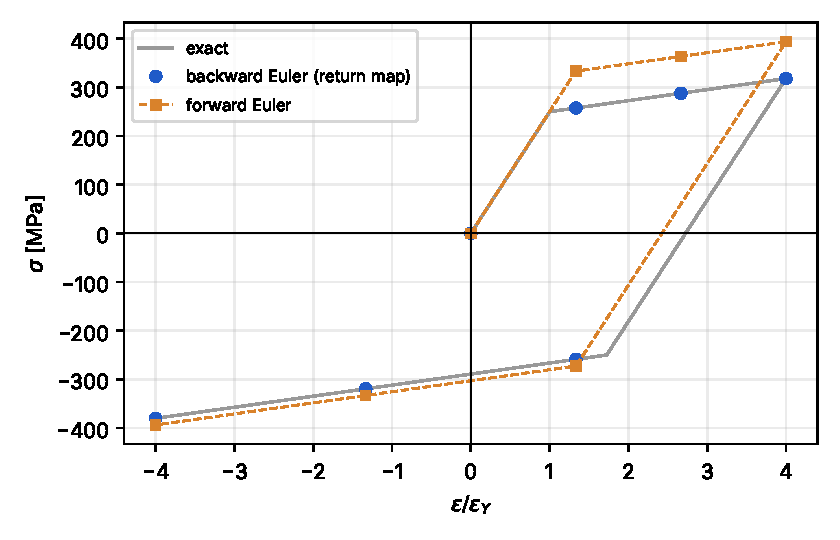
\includegraphics[width=0.62\textwidth]{figures/ch5/euler_filament.pdf}
\caption{Filament with combined hardening ($E=200$\,GPa, $\sY=250$\,MPa,
$K=H=10$\,GPa) under the strain cycle $0\to4\varepsilon_Y\to-4\varepsilon_Y$,
integrated with three steps per branch. Backward Euler (Box~5.1) lies on the
exact curve, the branches being monotone. Forward Euler overshoots the yield
stress in the first step that crosses it, and keeps the error: $393.9$\,MPa
instead of $318.2$\,MPa at the end of the first branch.}
\label{fig:pn-euler}
\end{figure}

%======================================================================
\section{Backward Euler is a closest-point projection}\label{sec:pn-cpp}
\index{closest-point projection}\index{backward Euler!as a projection}%
The plastic corrector of the filament moved the trial state onto the yield
surface. This section shows that, for every generalized standard material, the
corrector is the \emph{projection} of the trial state onto the elastic domain,
in the energy norm of~\eqref{eq:pl-energynorm}. We recall the projection onto
a convex set first~\cite{BauschkeCombettes2017,Moreau1965}.

\subsection{Projection onto a closed convex set}\label{ssec:pn-proj}
\index{projection onto a convex set}\index{non-expansive map}%
Let $X$ be a space with scalar product $\scal{\cdot}{\cdot}$ and norm
$\norm{\cdot}$ (finite dimensional here), and $\mathcal K\subset X$ a nonempty
closed convex set.
\begin{gbox}{Projection onto a convex set}
\begin{itemize}
  \item For every $\vx\in X$ there is a unique $P_{\mathcal K}\vx\in\mathcal K$ closest to $\vx$:
  $\displaystyle P_{\mathcal K}\vx=\argmin_{\vy\in\mathcal K}\tfrac12\norm{\vy-\vx}^2$.
  \item It is characterized by the variational inequality
  \begin{equation}\label{eq:pn-projVI}
    \vp=P_{\mathcal K}\vx\quad\Longleftrightarrow\quad
    \vp\in\mathcal K\ \text{ and }\ \scal{\vx-\vp}{\vy-\vp}\le0\quad\forall\vy\in\mathcal K,
  \end{equation}
  that is, $\vx-\vp$ belongs to the normal cone of $\mathcal K$ at $\vp$, for the
  scalar product $\scal{\cdot}{\cdot}$.
  \item $P_{\mathcal K}$ is \emph{firmly non-expansive}:
  $\norm{P_{\mathcal K}\vx-P_{\mathcal K}\vy}^2\le\scal{P_{\mathcal K}\vx-P_{\mathcal K}\vy}{\vx-\vy}$; in particular
  $\norm{P_{\mathcal K}\vx-P_{\mathcal K}\vy}\le\norm{\vx-\vy}$.
\end{itemize}
\end{gbox}
\paragraph{Why it works.} The squared distance
$\vy\mapsto\tfrac12\norm{\vy-\vx}^2$ is a bowl: strictly convex, and growing
at infinity. On a closed convex set it has exactly one lowest point
(Section~\ref{sec:var-direct}). At that point $\vp$, moving towards any other
point $\vy$ of $\mathcal K$ cannot bring us closer to $\vx$: the angle between
$\vx-\vp$ and $\vy-\vp$ is obtuse, which is~\eqref{eq:pn-projVI}. Draw a
convex body, a point outside and the foot of the perpendicular: every chord
from the foot points away from $\vx$. For the last item, write the angle
condition at $\vp=P_{\mathcal K}\vx$ towards $\vp'=P_{\mathcal K}\vy$, and at
$\vp'$ towards $\vp$, and add the two:
$\scal{(\vx-\vy)-(\vp-\vp')}{\vp'-\vp}\le0$. The Cauchy--Schwarz inequality
gives the Lipschitz bound. Two points are never farther apart than their
shadows on a convex set are close.

\subsection{The return map as a projection}\label{ssec:pn-cpp}
In the generalized variables of Section~\ref{sec:pl-gsm}, the forces are
$\vSig=(\sig,\vq)=-\partial_{\vz}\psi$, and with the quadratic free
energy~\eqref{eq:pl-psi} they are affine in $(\eps,\vz)$:
$\sig=\bbC:(\eps-\epsp)$, $\vq=-\bbD\valpha$. With
$\tensf{G}=\diag(\bbC,\bbD)$, a change $\Delta\vz$ of the internal variables
at fixed strain changes the forces by $-\tensf{G}\Delta\vz$. The \emph{trial
state} freezes the internal variables:
\begin{equation}\label{eq:pn-trial}
  \vSig^\trial_\np=\bigl(\bbC:(\eps_\np-\epsp_n),\ \vq_n\bigr)
  =\vSig_n+\bigl(\bbC:\Delta\eps,\ \vzero\bigr),
  \qquad
  \vSig_\np=\vSig^\trial_\np-\tensf{G}\,\Delta\vz .
\end{equation}
The scalar product of~\eqref{eq:pl-energynorm} is
$\scal{\vSig}{\vSig'}_E=\vSig\cdot\tensf{G}^{-1}\vSig'$, with
$\tensf{G}^{-1}=\diag(\bbS,\bbD^{-1})$: half the squared norm is the
complementary energy, elastic plus hardening.

Now comes the key fact of this chapter. For the filament, the corrector moved
the trial stress straight back to the yield surface. In every dimension, and
for every generalized standard material, it does the same thing: it goes to
the \emph{closest} admissible point.
\begin{gbox}{Backward Euler is a projection}\label{thm:pn-cpp}
The backward Euler step $\Delta\vz\in N_{\Esig}(\vSig_\np)$, with
$\vSig_\np=\vSig^\trial_\np-\tensf{G}\Delta\vz$, has exactly one solution:
the point of the elastic domain closest to the trial state, with the distance
measured in the energy norm,
\begin{equation}\label{eq:pn-cpp}
  \vSig_\np=P^E_{\Esig}\bigl(\vSig^\trial_\np\bigr)
  =\argmin_{\vSig^\ast\in\Esig}\ \tfrac12\norm{\vSig^\ast-\vSig^\trial_\np}_E^2,
  \qquad
  \Delta\vz=\tensf{G}^{-1}\bigl(\vSig^\trial_\np-\vSig_\np\bigr).
\end{equation}
\end{gbox}
\paragraph{Why it works.} Backward Euler asks for a plastic increment
$\Delta\vz$ normal to $\Esig$ at the \emph{end} point $\vSig_\np$: the angle
between $\Delta\vz$ and every chord $\vSig^\ast-\vSig_\np$ of the domain is
obtuse (Section~\ref{ssec:pl-cones}). Replace $\Delta\vz$ by
$\tensf{G}^{-1}(\vSig^\trial_\np-\vSig_\np)$:
\[
  \scal{\vSig^\trial_\np-\vSig_\np}{\vSig^\ast-\vSig_\np}_E\le0\qquad\text{for every }\vSig^\ast\in\Esig .
\]
This is the angle condition~\eqref{eq:pn-projVI} of the closest point, written
in the energy scalar product. The backward Euler equation and the projection
are one and the same equation. The closest point exists and is unique, and so
is the step. Simo and Hughes~\cite{SimoHughesCI} call this algorithm the
\emph{closest-point projection}.

\begin{figure}[h]
\centering
\begin{tikzpicture}[scale=1.15,>=Latex]
  \fill[cu!10,rotate=30] (0,0) ellipse (2.2 and 1.4);
  \draw[thick,cu,rotate=30] (0,0) ellipse (2.2 and 1.4);
  \node[cu] at (-0.5,0.0) {$\Esig$};
  \node[cu] at (-2.2,1.35) {$\partial\Esig$};
  \coordinate (Q) at (0.006,-1.516);
  \coordinate (P) at (1.659,1.376);
  \coordinate (T) at (2.747,2.811);
  \fill (Q) circle (1.6pt) node[below] {$\vSig_n$};
  \draw[->,thick] (Q) .. controls (2.6,-0.9) and (3.2,1.5) .. (T)
    node[pos=0.55,right,font=\small] {$\vSig_n+(\bbC:\Delta\eps,\vzero)$};
  \fill[orange!80!black] (T) circle (1.8pt) node[above right,orange!80!black] {$\vSig^\trial_\np$};
  \draw[->,very thick,orange!80!black] (T) -- ($(P)!0.06!(T)$);
  \fill[cu] (P) circle (1.8pt) node[left=2pt,cu] {$\vSig_\np$};
  \draw[dashed] ($(P)+1.6*(-0.797,0.604)$) -- ($(P)-1.4*(-0.797,0.604)$);
  \draw ($(P)+0.22*(0.604,0.797)$) -- ++($0.22*(-0.797,0.604)$) -- ++($-0.22*(0.604,0.797)$);
  \node[font=\small,orange!80!black,align=left] at (4.3,2.0) {$-\tensf{G}\Delta\vz$\\ (normal to $\partial\Esig$)};
\end{tikzpicture}
\caption{Closest-point projection, after Simo and
Hughes~\cite[Fig.~3.2]{SimoHughesCI}, drawn in coordinates where the energy
norm is Euclidean. The elastic predictor adds $\bbC:\Delta\eps$ to the stress
at fixed internal variables. The plastic corrector returns along the normal to
the yield surface at the \emph{final} point $\vSig_\np$: the trial state is
projected onto the elastic domain.}
\label{fig:pn-cpp}
\end{figure}

The projection is the discrete form of the principle of maximum plastic
dissipation (Section~\ref{thm:pl-maxdiss}): among all admissible forces,
$\vSig_\np$ maximizes $\vSig^\ast\cdot\Delta\vz$. It is also the principle of
minimum complementary energy of one step: the corrector looks for the
admissible force closest to the trial force, in the norm of the energy. Two
consequences are immediate. The elastic step is the case where the trial
state is admissible, since then it is its own projection. And the step
cannot fail: whatever $\Delta\eps$, the discrete problem has exactly one
solution, which is the uniqueness used above for the exactness of the
filament.

When the elastic domain is described by a yield function, the projection
becomes a set of equations that a computer can solve.
\begin{gbox}{Return-mapping equations}\label{cor:pn-rm}
\index{Karush--Kuhn--Tucker conditions!discrete}%
If $\Esig=\{f\le0\}$ with $f$ convex, differentiable and $f(\vzero)<0$, the
projection~\eqref{eq:pn-cpp} is the solution of
\begin{equation}\label{eq:pn-rm}
  \vSig_\np=\vSig^\trial_\np-\dg\,\tensf{G}\,\partial_{\vSig}f(\vSig_\np),\qquad
  \dg\ge0,\quad f(\vSig_\np)\le0,\quad\dg\,f(\vSig_\np)=0 .
\end{equation}
The step is elastic if and only if $f(\vSig^\trial_\np)\le0$.
\end{gbox}
\noindent These are the Karush--Kuhn--Tucker conditions of the minimization
in~\eqref{eq:pn-cpp} (Section~\ref{sec:var-lagrange}), with $\dg$ as the
Lagrange multiplier of the constraint $f\le0$; the condition $f(\vzero)<0$
guarantees that the multiplier exists. An admissible trial state is its own
closest point, which gives $\dg=0$. The first equation contains the backward Euler form of the flow and
hardening rules~\eqref{eq:pl-box-flow}: $\Delta\epsp=\dg\,\partial_{\sig}f$ and
$\Delta\valpha=\dg\,\partial_{\vq}f$, both evaluated at the end of the step. The
normal is the one at the projected point, not at the trial point: this is
what makes the scheme implicit. For a general yield function~\eqref{eq:pn-rm}
is a nonlinear system for $(\vSig_\np,\dg)$, solved by Newton's method on the
active constraint $f(\vSig_\np)=0$~\cite[Sec.~3.2]{SimoHughesCI}; the
\emph{cutting-plane} algorithm of Ortiz and Simo~\cite{OrtizSimo1986} avoids
the second derivatives of $f$ at the price of a linear rate of convergence.
For von Mises the system is solved in closed form.

%======================================================================
\section{\texorpdfstring{$J_2$}{J2} plasticity: radial return and consistent tangent}\label{sec:pn-j2}
\index{radial return}\index{J2 flow theory@$J_2$ flow theory!radial return}%
Take the $J_2$ model~\eqref{eq:pl-j2-f}--\eqref{eq:pl-j2-flow}, with isotropic
elasticity $\bbC=\kappa\,\tI\otimes\tI+2\mu\bbIdev$, linear kinematic hardening
$H$ and an isotropic hardening law $R(\alpha)$, linear ($R=\sY+K\alpha$) or not:
\[
  f(\sig,\tbeta,\alpha)=\norm{\dev\sig-\tbeta}-\sqrt{\tfrac23}\,R(\alpha),\qquad
  \Delta\epsp=\dg\,\tn_\np,\quad \Delta\tbeta=\tfrac23H\dg\,\tn_\np,\quad
  \Delta\alpha=\sqrt{\tfrac23}\,\dg,
\]
with $\tn_\np=\teta_\np/\norm{\teta_\np}$ and $\teta=\dev\sig-\tbeta$. For
this model the projection can be done by hand. The idea goes back to
Wilkins~\cite{Wilkins1964} and to Krieg and Key~\cite{KriegKey1976}.

\begin{gbox}{Radial return}\label{prop:pn-radial}
Let $\tens{s}^\trial=2\mu\dev(\eps_\np-\epsp_n)$,
$\teta^\trial=\tens s^\trial-\tbeta_n$ and
$f^\trial=\norm{\teta^\trial}-\sqrt{2/3}\,R(\alpha_n)$. If $f^\trial>0$, the
corrected state keeps the direction of the trial relative stress and only
shortens it:
\begin{equation}\label{eq:pn-radial}
  \tn_\np=\frac{\teta^\trial}{\norm{\teta^\trial}},\qquad
  \sig_\np=\sig^\trial_\np-2\mu\dg\,\tn_\np,
\end{equation}
where $\dg>0$ is the root of the scalar equation
\begin{equation}\label{eq:pn-radial-g}
  g(\dg):=\norm{\teta^\trial}-\bigl(2\mu+\tfrac23H\bigr)\dg-\sqrt{\tfrac23}\,R\Bigl(\alpha_n+\sqrt{\tfrac23}\dg\Bigr)=0 .
\end{equation}
For linear hardening, $\dg=f^\trial/\bigl(2\mu+\tfrac23(K+H)\bigr)$. The
pressure is not affected: $\tr\sig_\np=\tr\sig^\trial_\np=3\kappa\tr\eps_\np$.
\end{gbox}
\paragraph{Why it works.} Two observations do everything. First, the plastic
strain increment is deviatoric, so the pressure never sees plasticity.
Second, subtract the updates of $\tens s$ and $\tbeta$:
\[
  \teta_\np=\teta^\trial-\bigl(2\mu+\tfrac23H\bigr)\dg\,\tn_\np
  \quad\Longrightarrow\quad
  \Bigl[\norm{\teta_\np}+\bigl(2\mu+\tfrac23H\bigr)\dg\Bigr]\tn_\np=\teta^\trial .
\]
The bracket is a positive number, so the final normal $\tn_\np$ points along
$\teta^\trial$. The normal at the end of the step is known before the step is
computed! The only unknown left is the length $\dg$, and $f_\np=0$
is~\eqref{eq:pn-radial-g}. The function $g$ starts at $g(0)=f^\trial>0$ and
decreases to $-\infty$ ($R$ is non-decreasing): it crosses zero exactly once.

The return is \emph{radial}: in the deviatoric plane, the corrector moves the
trial stress along the radius of the von Mises circle centred at $\tbeta_n$
(Figure~\ref{fig:pn-radial}). It is the projection of
Section~\ref{thm:pn-cpp}: the energy norm on deviators is
$\norm{\tens s}^2/(2\mu)$, proportional to the Euclidean one, and the closest
point of a circle is along the radius. For nonlinear hardening the scalar
equation~\eqref{eq:pn-radial-g} is solved by Newton's method from $\dg=0$;
since $g$ is decreasing and convex for a saturating law (Voce), the iterates
increase monotonically to the root (Exercise~\ref{exo:pn-radial}).

\begin{gbox}{Box 5.2\quad Radial return for \texorpdfstring{$J_2$}{J2} plasticity}
\index{radial return!Box 5.2}%
\begin{enumerate}[label=\textbf{\arabic*.},leftmargin=1.6em]
  \item \textbf{Database.} Read $\epsp_n$, $\tbeta_n$, $\alpha_n$; the strain
  $\eps_\np$ is given.
  \item \textbf{Elastic predictor.}
  \[
    \tens s^\trial=2\mu\dev(\eps_\np-\epsp_n),\qquad
    \teta^\trial=\tens s^\trial-\tbeta_n,\qquad
    f^\trial=\norm{\teta^\trial}-\sqrt{\tfrac23}\,R(\alpha_n).
  \]
  \item \textbf{Check.} If $f^\trial\le0$: $\sig_\np=\kappa(\tr\eps_\np)\tI+\tens s^\trial$,
  internal variables unchanged, tangent $\bbC$; exit.
  \item \textbf{Multiplier.} Solve $g(\dg)=0$, equation~\eqref{eq:pn-radial-g}:
  in closed form for linear hardening, otherwise by Newton,
  \[
    \dg\leftarrow\dg+\frac{g(\dg)}{2\mu+\tfrac23\bigl(H+R'(\alpha_n+\sqrt{2/3}\,\dg)\bigr)} .
  \]
  \item \textbf{Update.} With $\tn=\teta^\trial/\norm{\teta^\trial}$:
  \[
    \sig_\np=\kappa(\tr\eps_\np)\tI+\tens s^\trial-2\mu\dg\,\tn,
  \]
  \[
    \epsp_\np=\epsp_n+\dg\,\tn,\quad
    \tbeta_\np=\tbeta_n+\tfrac23H\dg\,\tn,\quad
    \alpha_\np=\alpha_n+\sqrt{\tfrac23}\,\dg .
  \]
  \item \textbf{Consistent tangent.} Equation~\eqref{eq:pn-calg} below.
\end{enumerate}
\end{gbox}

\begin{figure}[h]
\centering
\begin{tikzpicture}[scale=1.0,>=Latex]
  \begin{scope}
  \fill[cu!10] (0,0) circle (1.8);
  \draw[thick,cu] (0,0) circle (1.8);
  \fill (0,0) circle (1.5pt) node[above left] {$\tbeta_n$};
  \coordinate (T) at (35:3.0);
  \coordinate (P) at (35:1.8);
  \draw[->,thin,gray] (0,0) -- (T);
  \fill[orange!80!black] (T) circle (1.8pt) node[above right,orange!80!black] {$\dev\sig^\trial_\np$};
  \draw[->,very thick,orange!80!black] (T) -- ($(P)!0.05!(T)$);
  \fill[cu] (P) circle (1.8pt) node[left=3pt,cu] {$\dev\sig_\np$};
  \node[font=\small,orange!80!black] at (3.35,1.25) {$-2\mu\dg\,\tn$};
  \draw[<->,gray] (0,0) -- (200:1.8);
  \node[gray,font=\scriptsize] at (-0.75,-0.65) {$\sqrt{\tfrac23}\,R(\alpha_n)$};
  \draw[dashed,cu!70] (0,0) circle (2.05);
  \node[font=\scriptsize,cu!80] at (-1.15,-1.95) {after hardening};
  \node[font=\small] at (0.6,-2.6) {(a) von Mises: radial return};
  \end{scope}
  \begin{scope}[xshift=8.0cm]
  \def\R{1.8}
  \fill[cu!10] (90:\R) -- (30:\R) -- (-30:\R) -- (-90:\R) -- (-150:\R) -- (150:\R) -- cycle;
  \draw[thick,cu] (90:\R) -- (30:\R) -- (-30:\R) -- (-90:\R) -- (-150:\R) -- (150:\R) -- cycle;
  \foreach \a in {90,30,-30,-90,-150,150}{
    \fill[orange!18] (\a:\R) -- ++(\a-30:1.0) arc[start angle=\a-30,end angle=\a+30,radius=1.0] -- cycle;}
  \draw[->,gray] (0,0) -- (90:2.9) node[above,font=\scriptsize] {$\sigma_1$};
  \draw[->,gray] (0,0) -- (210:2.9) node[below left,font=\scriptsize] {$\sigma_2$};
  \draw[->,gray] (0,0) -- (330:2.9) node[below right,font=\scriptsize] {$\sigma_3$};
  % face return
  \coordinate (F) at ($(0:{\R*cos(30)})+(90:0.35)$);
  \coordinate (Ft) at ($(F)+(0:1.1)$);
  \fill[orange!80!black] (Ft) circle (1.6pt);
  \draw[->,very thick,orange!80!black] (Ft) -- ($(F)+(0:0.06)$);
  \fill[cu] (F) circle (1.6pt);
  % corner return
  \coordinate (V) at (90:\R);
  \coordinate (Vt) at ($(V)+(100:0.95)$);
  \fill[orange!80!black] (Vt) circle (1.6pt);
  \draw[->,very thick,orange!80!black] (Vt) -- ($(V)!0.07!(Vt)$);
  \fill[cu] (V) circle (1.6pt);
  \node[font=\scriptsize,align=left] at (3.0,0.9) {face\\ return};
  \node[font=\scriptsize,align=left] at (-1.25,2.55) {corner\\ return};
  \node[font=\small] at (0.3,-2.6) {(b) Tresca: faces and corners};
  \end{scope}
\end{tikzpicture}
\caption{Returns in the deviatoric plane. (a) Von Mises: the corrector is
radial, along $\tn=\teta^\trial/\norm{\teta^\trial}$, onto the circle of
radius $\sqrt{2/3}\,R(\alpha_\np)$. (b) Tresca: a trial state in front of a
face returns along the normal to that face; a trial state in the cone of
normals of a vertex (orange) returns to the vertex
(Section~\ref{sec:pn-multi}).}
\label{fig:pn-radial}
\end{figure}

\subsection{The consistent tangent}\label{ssec:pn-calg}
\index{consistent tangent}\index{tangent modulus!consistent (algorithmic)}%
The return map defines the stress at $t_\np$ as a function of the strain at
$t_\np$, at fixed $\vz_n$. Its derivative
$\bbCalg=\partial\sig_\np/\partial\eps_\np$ is the \emph{consistent} (or
algorithmic) tangent of Simo and Taylor~\cite{SimoTaylor1985}; it is the
matrix that linearizes the discrete global problem
(Section~\ref{sec:pn-newton}). The continuum tangent $\bbCep$
of~\eqref{eq:pl-j2-cep} linearizes the rate equations instead.

\begin{gbox}{Consistent tangent of the radial return}\label{prop:pn-calg}
In a plastic step, with $\theta=1-2\mu\dg/\norm{\teta^\trial}$ and
$\displaystyle \bar\theta=\Bigl(1+\frac{R'(\alpha_\np)+H}{3\mu}\Bigr)^{-1}-(1-\theta)$,
\begin{equation}\label{eq:pn-calg}
  \bbCalg=\kappa\,\tI\otimes\tI+2\mu\theta\,\bbIdev-2\mu\bar\theta\,\tn\otimes\tn .
\end{equation}
It is symmetric, and it tends to the continuum tangent $\bbCep$ as $\dg\to0$.
\end{gbox}
\paragraph{Why it works.} The stress after the return,
$\sig_\np=\kappa(\tr\eps_\np)\tI+\tens s^\trial-2\mu\dg\,\tn$, depends on
$\eps_\np$ through three pieces: the trial deviator, the normal and the
multiplier. Differentiate each piece. The trial deviator gives
$\partial\tens s^\trial/\partial\eps_\np=2\mu\bbIdev$. The normal is a unit
tensor; it can only turn, and the derivative of a unit tensor
(Exercise~\ref{exo:pl-perfect3d}) gives
$\partial\tn/\partial\eps_\np=\dfrac{2\mu}{\norm{\teta^\trial}}\bigl(\bbIdev-\tn\otimes\tn\bigr)$.
The multiplier follows from $g(\dg)=0$, differentiated with
$\partial\norm{\teta^\trial}/\partial\eps_\np=2\mu\tn$:
\[
  2\mu\,\tn-\Bigl(2\mu+\tfrac23H+\tfrac23R'(\alpha_\np)\Bigr)\frac{\partial\dg}{\partial\eps_\np}=\vzero
  \quad\Longrightarrow\quad
  \frac{\partial\dg}{\partial\eps_\np}=\frac{\tn}{1+\frac{R'+H}{3\mu}} .
\]
Collecting,
$\bbCalg=\kappa\tI\otimes\tI+2\mu\bbIdev-2\mu\,\tn\otimes\partial\dg/\partial\eps_\np-2\mu\dg\,\partial\tn/\partial\eps_\np$,
which is~\eqref{eq:pn-calg} after writing $2\mu\dg/\norm{\teta^\trial}=1-\theta$.
Both rank-one terms are dyads of a tensor with itself: the tangent is
symmetric. A vanishing step gives $\theta=1$ and
$\bar\theta=(1+(R'+H)/(3\mu))^{-1}$, which is~\eqref{eq:pl-j2-cep}.
The two tangents differ by the factor $\theta<1$ on the deviatoric directions
orthogonal to $\tn$:
\[
  \bbCalg=\bbCep-2\mu(1-\theta)\bigl(\bbIdev-\tn\otimes\tn\bigr).
\]
The consistent tangent is softer in the directions that rotate the normal. The
reason is geometric: over a finite step, a strain increment orthogonal to
$\tn$ rotates the trial stress, and the radial return then shortens it by
$2\mu\dg$; the continuum tangent, which describes an infinitesimal step, does
not see this. The correction is not small: $1-\theta=2\mu\dg/\norm{\teta^\trial}$
is the fraction of the trial deviator removed by the corrector, close to one
for large steps in perfect plasticity. The eigenvalues of $\bbCalg$ are $3\kappa$
(on $\tI$), $2\mu(\theta-\bar\theta)=2\mu\,\dfrac{R'+H}{3\mu+R'+H}$ (on $\tn$) and $2\mu\theta$
(on the deviators orthogonal to $\tn$); they are positive with hardening.

%======================================================================
\section{The global Newton method}\label{sec:pn-newton}
\index{Newton's method!global equilibrium}%
The global equation~\eqref{eq:pn-residual} is solved by Newton's method. From
an estimate $\mat{u}^{(k)}$, linearize the residual,
$\mat{R}(\mat{u}^{(k)}+\delta\mat{u})\approx\mat{R}(\mat{u}^{(k)})-\mat{K}^{(k)}\delta\mat{u}$,
and solve the linear system
\begin{equation}\label{eq:pn-newton}
  \mat{K}^{(k)}\,\delta\mat{u}=\mat{R}(\mat{u}^{(k)}),\qquad
  \mat{K}^{(k)}=\frac{\partial\mat{F}^{\mathrm{int}}}{\partial\mat{u}}\Bigr|_{\mat{u}^{(k)}}
  =\sum_e\int_{\Omega_e}\mat{B}\T\,\mat{C}^{\mathrm{alg}}\,\mat{B}\dd x,
  \qquad \mat{u}^{(k+1)}=\mat{u}^{(k)}+\delta\mat{u} .
\end{equation}
The tangent stiffness is the derivative of the internal forces, and the chain
rule puts at each Gauss point the derivative of the stress \emph{delivered by
the return map} with respect to the strain: the consistent tangent $\bbCalg$
(in matrix form $\mat{C}^{\mathrm{alg}}$). Newton's method converges
quadratically near the solution only with this matrix~\cite{SimoTaylor1985}.

\begin{gbox}{Box 5.3\quad Incremental elastoplastic computation}
\index{Newton's method!Box 5.3}%
\begin{enumerate}[label=\textbf{\arabic*.},leftmargin=1.6em]
  \item \textbf{Step.} For $n=0,\dots,N-1$: apply the loads and the prescribed
  displacements of $t_\np$; start from $\mat{u}^{(0)}=\mat{u}_n$.
  \item \textbf{Local stage.} At each Gauss point, compute
  $\eps^{(k)}=\mat{B}\mat{u}^{(k)}$ and call the return map
  $(\sig^{(k)},\vz^{(k)},\bbCalg)=\mathcal R(\eps^{(k)};\vz_n)$, always from the
  converged internal variables $\vz_n$ of the previous step.
  \item \textbf{Assembly.}
  $\mat{F}^{\mathrm{int}}=\sum_e\int\mat{B}\T\sig^{(k)}$, $\mat{R}^{(k)}=\mat{F}^{\mathrm{ext}}_\np-\mat{F}^{\mathrm{int}}$,
  $\mat{K}^{(k)}=\sum_e\int\mat{B}\T\mat{C}^{\mathrm{alg}}\mat{B}$.
  \item \textbf{Convergence test.} If $\norm{\mat{R}^{(k)}}\le\mathrm{tol}\,\norm{\mat{F}^{\mathrm{ext}}_\np}$:
  store $\mat{u}_\np=\mat{u}^{(k)}$ and $\vz_\np=\vz^{(k)}$ at every Gauss
  point, and go to the next step.
  \item \textbf{Newton update.} Solve $\mat{K}^{(k)}\delta\mat{u}=\mat{R}^{(k)}$,
  set $\mat{u}^{(k+1)}=\mat{u}^{(k)}+\delta\mat{u}$, and return to stage~2.
\end{enumerate}
\end{gbox}
\noindent Figure~\ref{fig:pn-loop} draws the two nested loops of Box~5.3: the
outer loop on the load steps, and the inner Newton loop, which calls the local
stage at every iteration.

\begin{figure}[h]
\centering
\begin{tikzpicture}[>=Latex,node distance=5mm,
  fbox/.style={rectangle,rounded corners=2pt,fill=gray!12,align=flush center,
    inner sep=4pt,font=\small,text width=#1},fbox/.default=7.6cm,
  test/.style={diamond,aspect=2.6,fill=orange!14,align=flush center,inner sep=1pt,
    font=\small}]
  \node[fbox] (step) {\textbf{1. Step} $n\to n+1$: loads of $t_\np$;\\
    start from $\mat{u}^{(0)}=\mat{u}_n$, $k=0$};
  \node[fbox,kin,below=of step] (loc) {\textbf{2. Local stage}, at each Gauss point:\\
    $(\sig^{(k)},\vz^{(k)},\bbCalg)=\mathcal R\bigl(\mat{B}\mat{u}^{(k)};\,\vz_n\bigr)$};
  \node[fbox,stat,below=of loc] (asm) {\textbf{3. Assembly}:
    $\mat{F}^{\mathrm{int}}$, $\mat{R}^{(k)}=\mat{F}^{\mathrm{ext}}_\np-\mat{F}^{\mathrm{int}}$, $\mat{K}^{(k)}$};
  \node[test,below=of asm] (cv) {\textbf{4.} $\norm{\mat{R}^{(k)}}\le\mathrm{tol}\,\norm{\mat{F}^{\mathrm{ext}}_\np}$\,?};
  \node[fbox=3.7cm,right=8mm of cv] (nw) {\textbf{5. Newton update}\\
    $\mat{K}^{(k)}\delta\mat{u}=\mat{R}^{(k)}$\\ $\mat{u}^{(k+1)}=\mat{u}^{(k)}+\delta\mat{u}$};
  \node[fbox=3.5cm,left=8mm of cv] (acc) {\textbf{Accept}\\
    $\mat{u}_\np=\mat{u}^{(k)}$, $\vz_\np=\vz^{(k)}$\\ at every Gauss point};
  \draw[arr] (step) -- (loc);
  \draw[arr] (loc) -- (asm);
  \draw[arr] (asm) -- (cv);
  \draw[arr] (cv) -- node[above,font=\small] {no} (nw);
  \draw[arr] (cv) -- node[above,font=\small] {yes} (acc);
  \draw[arr] (nw.north) |- node[pos=0.3,right,font=\small,align=left] {$k\gets k+1$\\[-1pt]{\footnotesize\sffamily\color{gray}Newton}} (loc.east);
  \draw[arr] (acc.north) |- node[pos=0.3,left,font=\small,align=right] {$n\gets n+1$\\[-1pt]{\footnotesize\sffamily\color{gray}next step}} (step.west);
\end{tikzpicture}
\caption{The global/local loop of Box~5.3. The local stage (blue) integrates
the flow rule at each Gauss point, always from the converged internal
variables $\vz_n$; the assembly (green) restores equilibrium. The Newton loop
on the right repeats stages 2--5 at fixed $t_\np$; the loop on the left
advances the load step once the residual is small.}
\label{fig:pn-loop}
\end{figure}

\paragraph{Path independence within a step.}
\index{return map!from the converged state}%
The return map in stage~2 starts from $\vz_n$, not from the internal
variables of the previous iterate. The iterates $\mat{u}^{(k)}$ are not states
of the material: they are guesses of the end point of the step, and the
backward Euler step is a function of $(\eps_\np,\vz_n)$ only. Updating the
internal variables from iterate to iterate would make the result depend on the
convergence history and would accumulate spurious plastic strain. Each Gauss
point therefore stores two sets of internal variables: the converged values
of $t_n$ and the current ones.

\paragraph{Consistent against continuum tangent.}
Figure~\ref{fig:pn-newton} compares the two tangents on the thick-walled
cylinder of Exercise~\ref{exo:pl-cyl}, now with Voce hardening and computed
with finite elements (Exercise~\ref{exo:pn-tangent}). With $\bbCalg$ the
residual is squared at each iteration near the solution; with $\bbCep$ it
decreases by a constant factor. Both converge to the same displacement, to
ten digits: the tangent changes the path to the solution, not the solution,
which is fixed by the residual. The first iterations of a step use the elastic
tangent at points that are about to yield, which explains the initial increase
of the residual; a line search on the energy of Section~\ref{sec:pn-var}
prevents it.

\begin{figure}[h]
\centering
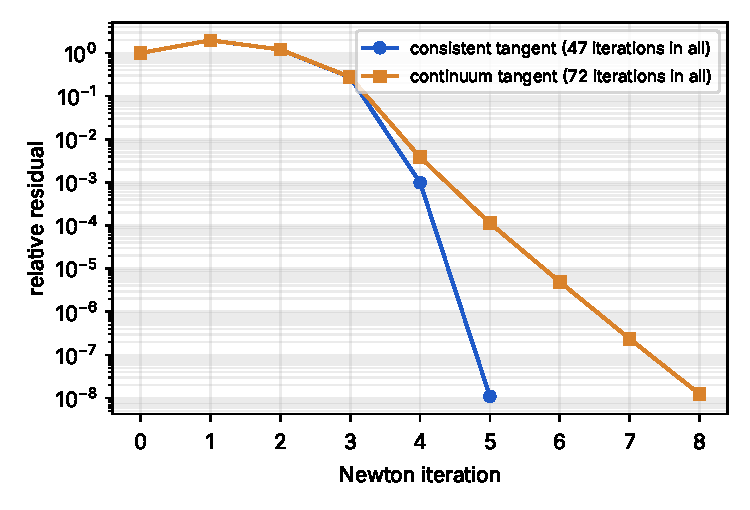
\includegraphics[width=0.6\textwidth]{figures/ch5/newton.pdf}
\caption{Newton iterations in load step 6 of 10 for the thick-walled cylinder
($a=100$, $b=200$\,mm, plane strain, Voce hardening, $p=320$\,MPa, 80
elements). Relative residual against the iteration number with the
consistent tangent (quadratic convergence) and with the continuum tangent
(linear convergence, ratio about $0.05$ per iteration). Over the ten steps
the consistent tangent needs 47 iterations and the continuum one 72.}
\label{fig:pn-newton}
\end{figure}

%======================================================================
\section{Corners: multi-surface plasticity and active sets}\label{sec:pn-multi}
\index{multi-surface plasticity}\index{active set}\index{Tresca criterion!return map}%
When the elastic domain is an intersection of smooth domains,
$\Esig=\bigcap_{\beta=1}^m\{f_\beta\le0\}$ (Tresca, Mohr--Coulomb, crystal
plasticity, caps), the projection property of Section~\ref{thm:pn-cpp} still holds: the solution is the
projection of the trial state. By the last item of the box of
Section~\ref{ssec:pl-cones}, the return-mapping equations~\eqref{eq:pn-rm}
become, with Koiter's rule,
\begin{equation}\label{eq:pn-rm-multi}
  \vSig_\np=\vSig^\trial_\np-\sum_{\beta}\dg^\beta\,\tensf{G}\,\partial_{\vSig}f_\beta(\vSig_\np),\qquad
  \dg^\beta\ge0,\quad f_\beta(\vSig_\np)\le0,\quad\dg^\beta f_\beta(\vSig_\np)=0 .
\end{equation}
The new unknown is the \emph{active set}
$J_\np=\{\beta:\ \dg^\beta>0\}$. It is not, in general, the set of the
surfaces violated by the trial state: a trial state can violate a surface and
return to a point where that surface is inactive. Simo, Kennedy and
Govindjee~\cite{SimoKennedyGovindjee1988} find it by the active-set strategy of
quadratic programming: start from the violated surfaces, solve the projection
with these constraints as equalities, drop the surfaces with a negative
multiplier, add the surfaces violated by the new state, and repeat. Because
the projection is a strictly convex problem, the stress $\vSig_\np$ is unique,
even when the gradients of the active surfaces are linearly dependent and the
multipliers are not.

\paragraph{Tresca in principal stresses.}
For isotropic elasticity and an isotropic criterion, the return does not
rotate the principal axes of the trial stress: the trial deviator, its
projection and the normals are coaxial. The return can therefore be computed
on the ordered principal values $s_1\ge s_2\ge s_3$ of $\sig^\trial_\np$. For
perfect Tresca plasticity the face $f_a=\sigma_1-\sigma_3-\sY$ has the
normal $\tens N_a=\ve_1\otimes\ve_1-\ve_3\otimes\ve_3$ (in the principal
basis), with $\tens N_a:\bbC:\tens N_a=4\mu$. At a vertex two faces are active,
and $\tens N_a:\bbC:\tens N_b=2\mu$ for adjacent faces.

\begin{gbox}{Box 5.4\quad Return map for Tresca (perfect plasticity)}
\index{Tresca criterion!Box 5.4}%
\begin{enumerate}[label=\textbf{\arabic*.},leftmargin=1.6em]
  \item \textbf{Predictor.} Compute $\sig^\trial_\np=\bbC:(\eps_\np-\epsp_n)$, its
  principal values $s_1\ge s_2\ge s_3$ and directions, and $f_a=s_1-s_3-\sY$.
  If $f_a\le0$, the step is elastic.
  \item \textbf{Face return.} $\dg=f_a/(4\mu)$,
  $\sigma_1=s_1-2\mu\dg$, $\sigma_2=s_2$, $\sigma_3=s_3+2\mu\dg$. If
  $\sigma_1\ge\sigma_2\ge\sigma_3$, accept.
  \item \textbf{Corner $\sigma_1=\sigma_2$} (when $s_2>\sigma_1$). With
  $f_b=s_2-s_3-\sY$:
  \[
    \dg^a=\frac{2f_a-f_b}{6\mu},\qquad \dg^b=\frac{2f_b-f_a}{6\mu},
  \]
  \[
    \sigma_1=s_1-2\mu\dg^a,\quad\sigma_2=s_2-2\mu\dg^b,\quad\sigma_3=s_3+2\mu(\dg^a+\dg^b).
  \]
  \item \textbf{Corner $\sigma_2=\sigma_3$} (when $s_2<\sigma_3$). With
  $f_b=s_1-s_2-\sY$ and the same $\dg^a,\dg^b$:
  $\sigma_1=s_1-2\mu(\dg^a+\dg^b)$, $\sigma_2=s_2+2\mu\dg^b$, $\sigma_3=s_3+2\mu\dg^a$.
  \item \textbf{Update.} Rebuild $\sig_\np$ on the principal directions of the
  trial stress, and $\epsp_\np=\epsp_n+\bbS:(\sig^\trial_\np-\sig_\np)$.
\end{enumerate}
\end{gbox}
\noindent The test of stage~2 is the sign of $\dg^b$: the vertex is the
correct return if and only if $2f_b>f_a$, that is, if the trial state lies in
the cone of normals of the vertex (Figure~\ref{fig:pn-radial}b and
Exercise~\ref{exo:pn-tresca}). The return is continuous across the boundary of
that cone, but its derivative is not: the consistent tangent jumps, from a
tangent with one zero eigenvalue (face) to one with two (vertex).

%======================================================================
\section{Plane stress: the projected return}\label{sec:pn-ps}
\index{plane stress!return map}\index{projected return}%
In plates, shells and membranes the stress is plane, $\sigma_{33}=\sigma_{13}=\sigma_{23}=0$,
and the out-of-plane strain $\varepsilon_{33}$ is an unknown. The
three-dimensional radial return cannot be applied directly, because the trial
deviator would need $\varepsilon_{33}$. One option is to iterate on
$\varepsilon_{33}$ until $\sigma_{33}=0$ around the three-dimensional return.
Simo and Taylor~\cite{SimoTaylor1986} work instead in the plane-stress subspace,
with the vectors $\vect{\sigma}=(\sigma_{11},\sigma_{22},\sigma_{12})$ and
$\vect{\varepsilon}=(\varepsilon_{11},\varepsilon_{22},2\varepsilon_{12})$, the
plane-stress moduli and the von Mises matrix
\[
  \mat{C}=\frac{E}{1-\nu^2}\begin{bmatrix}1&\nu&0\\ \nu&1&0\\ 0&0&\tfrac{1-\nu}{2}\end{bmatrix},
  \qquad
  \mat{P}=\frac13\begin{bmatrix}2&-1&0\\ -1&2&0\\ 0&0&6\end{bmatrix},
  \qquad
  \vect{\sigma}\T\mat{P}\vect{\sigma}=\norm{\dev\sig}^2=2J_2 .
\]
For isotropic hardening the yield function is
$f=\tfrac12\vect{\sigma}\T\mat{P}\vect{\sigma}-\tfrac13R(\alpha)^2$, and the
backward Euler step reads
\begin{equation}\label{eq:pn-ps}
  \vect{\sigma}_\np=\vect{\sigma}^\trial_\np-\dg\,\mat{C}\mat{P}\vect{\sigma}_\np
  \quad\Longrightarrow\quad
  \vect{\sigma}_\np=\bigl(\mat{I}+\dg\,\mat{C}\mat{P}\bigr)^{-1}\vect{\sigma}^\trial_\np,
  \quad
  \alpha_\np=\alpha_n+\sqrt{\tfrac23}\,\dg\,\varphi(\dg),
\end{equation}
with $\varphi=\sqrt{\vect{\sigma}_\np\T\mat{P}\vect{\sigma}_\np}=\norm{\dev\sig_\np}$.
The return is \emph{not} radial: $\mat{C}\mat{P}$ is not a multiple of the
identity. But $\mat{C}$ and $\mat{P}$ have the same eigenvectors,
$(1,1,0)/\sqrt2$, $(-1,1,0)/\sqrt2$ and $(0,0,1)$, with eigenvalues
$E/(1-\nu)$, $2\mu$, $\mu$ for $\mat{C}$ and $\tfrac13$, $1$, $2$ for
$\mat{P}$. In this basis the inverse is diagonal, and the whole return
reduces to one scalar equation (Exercise~\ref{exo:pn-ps}).
Figure~\ref{fig:pn-ps} shows the return in the plane of the principal
stresses. The yield locus is the ellipse
$\sigma_{11}^2-\sigma_{11}\sigma_{22}+\sigma_{22}^2=\sY^2$. A uniaxial trial
stress does not return to the uniaxial point: the corrector follows
$\mat{C}\mat{P}\vect{\sigma}_\np$, which is the normal in the energy norm but
neither the radius nor the Euclidean normal $\mat{P}\vect{\sigma}_\np$.

\begin{gbox}{Box 5.5\quad Projected return for plane stress}
\index{plane stress!Box 5.5}%
\begin{enumerate}[label=\textbf{\arabic*.},leftmargin=1.6em]
  \item \textbf{Predictor.} $\vect{\sigma}^\trial=\mat{C}(\vect{\varepsilon}_\np-\vect{\varepsilon}^p_n)$;
  if $\tfrac12\vect{\sigma}^{\trial\top}\mat{P}\vect{\sigma}^\trial\le\tfrac13R(\alpha_n)^2$, the step is elastic.
  \item \textbf{Modes.} For $\dg\ge0$,
  \[
    \varphi^2(\dg)=\frac{(\sigma^\trial_{11}+\sigma^\trial_{22})^2}{6\bigl(1+\frac{E\dg}{3(1-\nu)}\bigr)^2}
    +\frac{\tfrac12(\sigma^\trial_{22}-\sigma^\trial_{11})^2+2(\sigma^\trial_{12})^2}{(1+2\mu\dg)^2}.
  \]
  \item \textbf{Consistency.} Solve the scalar equation
  $\tfrac12\varphi^2(\dg)-\tfrac13R^2\bigl(\alpha_n+\sqrt{2/3}\,\dg\,\varphi(\dg)\bigr)=0$
  for $\dg>0$ (Newton, or bisection).
  \item \textbf{Update.} $\vect{\sigma}_\np=(\mat{C}^{-1}+\dg\mat{P})^{-1}\mat{C}^{-1}\vect{\sigma}^\trial$,
  $\vect{\varepsilon}^p_\np=\vect{\varepsilon}^p_n+\dg\,\mat{P}\vect{\sigma}_\np$,
  $\alpha_\np=\alpha_n+\sqrt{2/3}\,\dg\,\varphi(\dg)$; the thickness strain
  follows from $\sigma_{33}=0$.
\end{enumerate}
\end{gbox}
\noindent The plane-stress condition is satisfied exactly, without nested
iterations, which makes Box~5.5 the standard algorithm of shell elements. Its
consistent tangent is given in~\cite[Box~3.4]{SimoHughesCI}.

\begin{figure}[h]
\centering
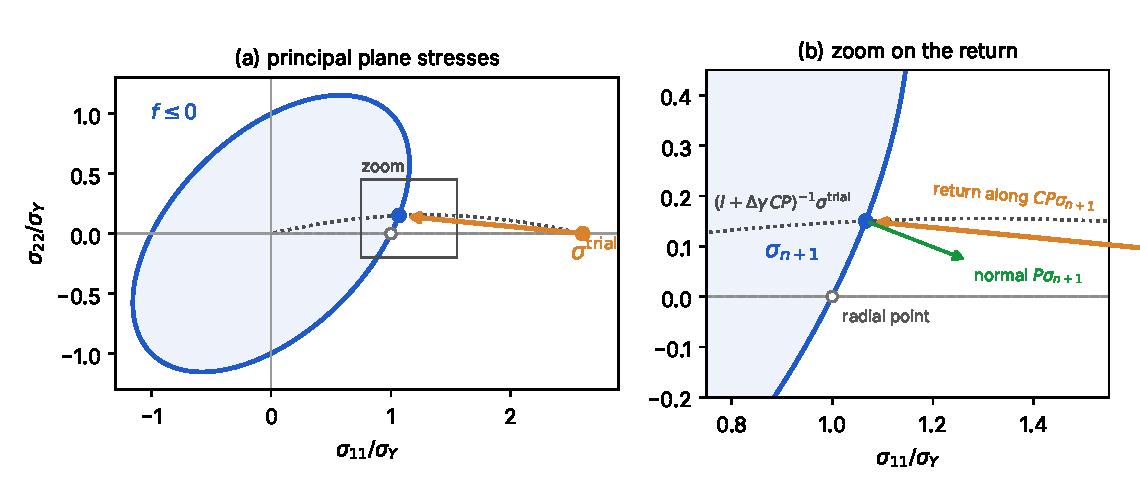
\includegraphics[width=\textwidth]{figures/ch5/plane_stress_return.pdf}
\caption{Projected return in plane stress (Box~5.5), perfect plasticity,
$\nu=0.3$, principal stresses ($\sigma_{12}=0$). (a) The trial stress
$\sigma^\trial=2.6\,\sY$ is uniaxial. The solution is sought on the curve
$\dg\mapsto(\mat{I}+\dg\,\mat{C}\mat{P})^{-1}\vect{\sigma}^\trial$ (dotted), which
crosses the ellipse at $\vect{\sigma}_\np=(1.067,\,0.150)\,\sY$; the radial
point $(1,0)\,\sY$ is not the solution. (b) Zoom: the straight return
$\vect{\sigma}^\trial-\vect{\sigma}_\np=\dg\,\mat{C}\mat{P}\vect{\sigma}_\np$
is not along the Euclidean normal $\mat{P}\vect{\sigma}_\np$ (green).}
\label{fig:pn-ps}
\end{figure}

%======================================================================
\section{Viscoplasticity}\label{sec:pn-vp}
\index{viscoplasticity!return map}%
In viscoplasticity the flow rule is a differential equation with a finite
right-hand side (Section~\ref{ssec:pl-gsm-def}), and backward Euler keeps the
time step.

\paragraph{Perzyna.}
\index{viscoplasticity!Perzyna}%
With the dual potential~\eqref{eq:pl-perzyna},
$\dot\vz=\eta^{-1}\mac{f(\vSig)}\,\partial_{\vSig}f$, the discrete multiplier
is no longer fixed by $f_\np=0$ but by
\begin{equation}\label{eq:pn-perzyna}
  \dg=\frac{\Delta t}{\eta}\,f(\vSig_\np)\qquad\text{(plastic step)}:
\end{equation}
the overstress at the end of the step is proportional to the multiplier. For
$J_2$ plasticity with linear hardening the radial return applies unchanged,
with
\begin{equation}\label{eq:pn-perzyna-j2}
  \dg=\frac{f^\trial}{2\mu+\tfrac23(K+H)+\eta/\Delta t} .
\end{equation}
The rate-independent return is recovered for $\eta\to0$, and also for
$\Delta t\to\infty$ at fixed $\eta$: over a long step the overstress has time to
relax. For $\eta/\Delta t$ large compared with $2\mu$, the step is nearly
elastic. The consistent tangent~\eqref{eq:pn-calg} holds with $R'+H$ replaced
by $R'+H+\tfrac32\eta/\Delta t$.

\paragraph{Duvaut--Lions.}
\index{viscoplasticity!Duvaut--Lions}%
The Duvaut--Lions model of Section~\ref{ssec:pl-gsm-def} relaxes the forces
towards their projection onto $\Esig$:
$\dot\vz=\tau^{-1}\tensf{G}^{-1}\bigl(\vSig-P^E_{\Esig}\vSig\bigr)$, with the
relaxation time $\tau$. Its backward Euler step is a simple modification of
the rate-independent one~\cite[Sec.~2.7]{SimoHughesCI}.
\begin{gbox}{Duvaut--Lions update}\label{prop:pn-dl}
Let $r=\Delta t/\tau$ and let $\bar\vSig_\np=P^E_{\Esig}(\vSig^\trial_\np)$ be
the rate-independent solution. The viscoplastic state lies on the segment
from the trial state to its projection:
\begin{equation}\label{eq:pn-dl}
  \vSig_\np=\frac{\vSig^\trial_\np+r\,\bar\vSig_\np}{1+r},
\end{equation}
and this is the only solution of the backward Euler step.
\end{gbox}
\paragraph{Why it works.} Look at Figure~\ref{fig:pn-dl}. With $P=P^E_{\Esig}$,
backward Euler asks $\tensf{G}\Delta\vz=r(\vSig_\np-P\vSig_\np)$, that is,
$(1+r)\vSig_\np-rP\vSig_\np=\vSig^\trial_\np$. Try a point on the segment
from $\bar\vSig_\np$ to the trial state. All the points of that segment have
the same closest point $\bar\vSig_\np$: sliding along the normal does not move
the foot of the perpendicular (this is~\eqref{eq:pn-projVI}). So
$P\vSig_\np=\bar\vSig_\np$, the equation becomes linear,
$(1+r)\vSig_\np-r\bar\vSig_\np=\vSig^\trial_\np$, and its solution
is~\eqref{eq:pn-dl}. There is no other solution: subtract the equations of two
solutions and use that $I-P$ is monotone (firm non-expansiveness); this gives
$(1+r)\norm{\vSig-\vSig'}_E^2-r\norm{\vSig-\vSig'}_E^2\le0$.
The viscoplastic state lies on the segment between the trial state ($r\to0$,
a very viscous or a very short step) and the projection ($r\to\infty$)
(Figure~\ref{fig:pn-dl}). Its distance to $\Esig$, the overstress, is the fraction
$\displaystyle \frac{1}{1+r}$ of the distance of the trial state. A
viscoplastic code is obtained from a plastic one with two extra lines.

\begin{figure}[h]
\centering
\begin{tikzpicture}[scale=1.1,>=Latex]
  \fill[cu!10] (0,0) ellipse (2.0 and 1.3);
  \draw[thick,cu] (0,0) ellipse (2.0 and 1.3);
  \node[cu] at (-0.6,-0.1) {$\Esig$};
  % P on the boundary (parameter 15 deg), unit normal n, perpendicular m
  \coordinate (P) at (1.932,0.336);
  \def\nx{0.925}\def\ny{0.381}
  \coordinate (T) at ($(P)+4.2*(\nx,\ny)$);
  \coordinate (S) at ($(P)!0.4!(T)$);
  \draw[dashed,gray] ($(P)+0.9*(-\ny,\nx)$) -- ($(P)-0.6*(-\ny,\nx)$);
  \draw[very thick,orange!80!black] (P) -- (T);
  \fill[orange!80!black] (T) circle (1.8pt) node[right=3pt,orange!80!black,align=left]
    {$\vSig^\trial_\np$\\ ($r\to0$)};
  \fill[cu] (P) circle (1.8pt) node[below right=6pt and 4pt,cu,align=left]
    {$\bar\vSig_\np=P^E_{\Esig}\vSig^\trial_\np$\\ ($r\to\infty$, plasticity)};
  \fill (S) circle (2.1pt) node[below right=2pt and 0pt] {$\vSig_\np$};
  \draw[decorate,decoration={brace,amplitude=5pt},thick,gray]
    ($(P)+0.15*(-\ny,\nx)$) -- ($(S)+0.15*(-\ny,\nx)$);
  \draw[decorate,decoration={brace,amplitude=5pt},thick,gray]
    ($(S)+0.15*(-\ny,\nx)$) -- ($(T)+0.15*(-\ny,\nx)$);
  \node[font=\small] at ($(P)!0.5!(S)+0.88*(-\ny,\nx)$) {$\dfrac{1}{1+r}$};
  \node[font=\small] at ($(S)!0.5!(T)+0.88*(-\ny,\nx)$) {$\dfrac{r}{1+r}$};
\end{tikzpicture}
\caption{Duvaut--Lions update~\eqref{eq:pn-dl}, drawn in coordinates where the
energy norm is Euclidean. The viscoplastic state is a point of the segment
joining the trial state to its projection $\bar\vSig_\np$ on the elastic
domain, with $r=\Delta t/\tau$; the brace labels are the fractions of the
length of the segment. Every point of the segment projects onto
$\bar\vSig_\np$, which is why the update needs only the rate-independent
return.}
\label{fig:pn-dl}
\end{figure}

%======================================================================
\section{Accuracy and stability}\label{sec:pn-stab}
\index{return map!accuracy}\index{return map!stability}\index{B-stability}%
\paragraph{Accuracy.}
\index{iso-error map}%
Backward Euler is first-order accurate: the local error over a step is
$O(\Delta t^2)$, the global error $O(\Delta t)$~\cite{OrtizPopov1985,SimoHughesCI}.
For the radial return the error comes from the rotation of the normal: the
exact solution integrates $\dot\epsp=\gamma\tn(t)$ with a turning $\tn$, the
algorithm uses the final normal for the whole step. The error vanishes when
the normal does not turn. Hence the radial return is exact on
\emph{proportional} paths with linear hardening (simple shear, uniaxial
tension, the filament on monotone steps), whatever the step size, and first
order on non-proportional paths (Exercise~\ref{exo:pn-shear}). The error over
one step is mapped by the \emph{iso-error maps} of Krieg and
Krieg~\cite{KriegKrieg1977} and Simo and Taylor~\cite{SimoTaylor1985}
(Figure~\ref{fig:pn-isoerror}): a strain increment along the normal produces
no error, an increment along the tangent the largest one. A useful rule
follows: steps of a few yield strains are acceptable on proportional
parts of a loading, and must be refined where the loading path turns. A
code that reproduces all the proportional calibration tests (tension, simple
shear, balanced biaxial tension) at one step per increment is correctly
programmed, but its step size is not validated.

\begin{figure}[h]
\centering
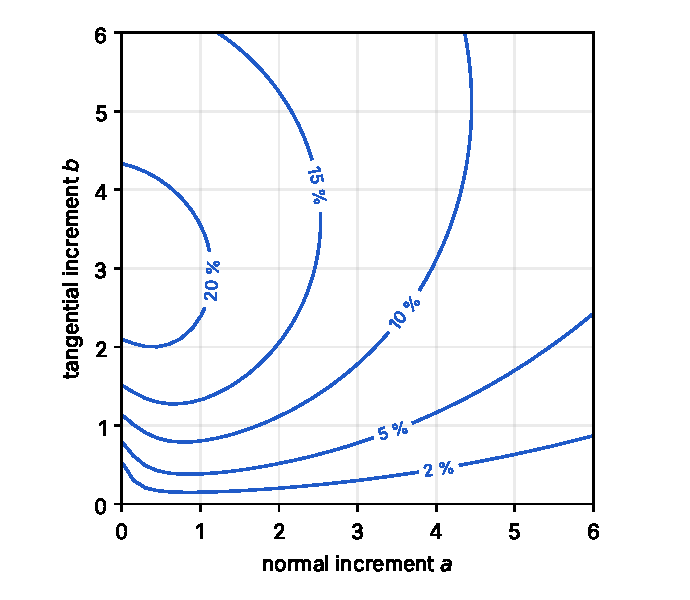
\includegraphics[width=0.5\textwidth]{figures/ch5/isoerror.pdf}
\caption{Iso-error map of the radial return, perfect $J_2$ plasticity, after
Simo and Taylor~\cite{SimoTaylor1985}. The initial state is on the yield
surface in uniaxial tension; one step of strain increment
$\Delta\eps=(a\,\tn+b\,\tens t)\,R/(2\mu)$, with $\tens t$ a unit deviator
orthogonal to $\tn$ and $R=\sqrt{2/3}\,\sY$, is compared with a solution with
1000 sub-steps. Contours: relative error on the deviatoric stress. The error
is zero for a normal increment ($b=0$) and largest for a tangential increment
of a few yield strains ($22\,\%$ at $a=0$, $b=3$).}
\label{fig:pn-isoerror}
\end{figure}

Second-order accuracy is obtained by the generalized midpoint rule, which
evaluates the normal at an intermediate point of the step; it is stable for
the midpoint parameter $\alpha\ge\tfrac12$ and second order for
$\alpha=\tfrac12$, but it gives up the projection structure and its
properties~\cite{OrtizPopov1985,SimoGovindjee1991}. In practice, step-size
control is preferred.

\paragraph{Stability.}
Plasticity is dissipative: two solutions driven by the same strain history do
not move apart in the energy norm (the argument for the uniqueness of the
stresses, Section~\ref{thm:pl-unique}, at a single point). A good algorithm
keeps this property for every step size.

\begin{gbox}{The return map never increases distances}\label{thm:pn-contract}
Drive two states $\vSig_n$ and $\vSig'_n$ with the same strain increment
$\Delta\eps$. After the return map they are not farther apart, in the energy
norm:
\[
  \norm{\vSig_\np-\vSig'_\np}_E\le\norm{\vSig_n-\vSig'_n}_E ,
\]
whatever the size of the step.
\end{gbox}
\paragraph{Why it works.} Two lines. The elastic predictor adds the same
$(\bbC:\Delta\eps,\vzero)$ to both states~\eqref{eq:pn-trial}, so the trial
states are exactly as far apart as the old states. The corrector projects
both onto the same convex set (Section~\ref{thm:pn-cpp}), and projections
never increase distances (Section~\ref{ssec:pn-proj}). Simo and
Govindjee~\cite{SimoGovindjee1991} call this property \emph{contractivity}.

The bound holds for every $\Delta\eps$: the return map is unconditionally
stable in the nonlinear sense (B-stability). Errors made in a step, for
instance by a loose tolerance of the global Newton iterations, are not
amplified by the following steps. Forward Euler has no such property. Take the
perfectly plastic filament with one state on the yield surface, $\sigma=\sY$,
and one inside, $\sigma'=\sY-\delta$, and a strain increment
$\Delta\varepsilon>2\delta/E$: forward Euler leaves $\sigma$ unchanged and
moves $\sigma'$ elastically to $\sY-\delta+E\Delta\varepsilon$, so that the
distance grows from $\delta$ to $E\Delta\varepsilon-\delta$; the return map
gives $\sigma_\np=\sigma'_\np=\sY$ (Exercise~\ref{exo:pn-contract}).

%======================================================================
\section{The incremental problem as a minimization}\label{sec:pn-var}
\index{variational constitutive update}\index{incremental potential}%
The projection of Section~\ref{thm:pn-cpp} describes the step by a
minimization over the \emph{forces}. The same step is also a minimization over
the \emph{internal variables}, and that one gives an energy for the whole
incremental problem. Here is the idea in words: one step of plasticity
chooses the internal variables that make the stored energy plus the
dissipated energy as small as possible. This is the variational constitutive
update of Ortiz and Stainier~\cite{OrtizStainier1999}; see
also~\cite{Miehe2002} and~\cite[Sec.~2.8]{KondoMaitournam2023b}.

\begin{gbox}{One step minimizes stored plus dissipated energy}\label{thm:pn-W}
For the quadratic free energy~\eqref{eq:pl-psi} and $\Esig$ closed convex with
$\vzero\in\Esig$, let
\begin{equation}\label{eq:pn-Wn}
  W_n(\eps)=\min_{\vz}\Bigl\{\psi(\eps,\vz)-\psi(\eps_n,\vz_n)+\pi_{\Esig}(\vz-\vz_n)\Bigr\},
\end{equation}
the change of free energy plus the dissipation of the step, minimized over the
internal variables. Then:
\begin{enumerate}[label=(\alph*)]
  \item the minimizer is $\vz_\np=\vz_n+\Delta\vz$, the backward Euler step;
  \item $W_n(\eps)=\psi(\eps,\vz_n)-\psi(\eps_n,\vz_n)-\tfrac12\,\mathrm{dist}_E\bigl(\vSig^\trial(\eps),\Esig\bigr)^2$;
  \item $W_n$ is convex and differentiable, and
  $\partial W_n/\partial\eps=\sig_\np$: the return map derives from a potential;
  \item where $W_n$ is twice differentiable,
  $\bbCalg=\partial^2W_n/\partial\eps^2$ is symmetric and positive
  semi-definite.
\end{enumerate}
\end{gbox}
\paragraph{Why it works.} (a) Write the increment as $\vect\zeta=\vz-\vz_n$.
Because $\psi$ is quadratic in $\vz$, the function to minimize is a bowl plus
the dissipation,
$\Phi(\vect\zeta)=\tfrac12\vect\zeta\cdot\tensf{G}\vect\zeta-\vSig^\trial\cdot\vect\zeta+\pi_{\Esig}(\vect\zeta)$,
up to a constant. At the bottom the slopes balance:
$\vSig^\trial-\tensf{G}\vect\zeta\in\partial\pi_{\Esig}(\vect\zeta)$. The force
at the end of the step is a slope of the dissipation function at the
increment. By the principle of maximum dissipation (Section~\ref{thm:pl-maxdiss},
forms (b) and (c)) this says that $\vect\zeta$ is normal to $\Esig$ at
$\vSig^\trial-\tensf{G}\vect\zeta$: it is the backward Euler step.
(b) At the bottom, the dissipation equals $\vSig_\np\cdot\Delta\vz$ (form (d)
of the same principle), and $\vSig_\np=\vSig^\trial-\tensf{G}\Delta\vz$, so
$\Phi(\Delta\vz)=-\tfrac12\Delta\vz\cdot\tensf{G}\Delta\vz=-\tfrac12\norm{\vSig^\trial-\vSig_\np}_E^2$.
(c) Minimizing a jointly convex function of $(\eps,\vz)$ over $\vz$ leaves a
convex function of $\eps$. For the gradient, the gradient of half a squared
distance to a convex set is the gap $\vSig-P^E_{\Esig}\vSig$, and the chain
rule gives
$\partial W_n/\partial\eps=\sig^\trial-\bbC:\bbS:(\sig^\trial-\sig_\np)=\sig_\np$.
(d) A Hessian is always symmetric, and it is positive semi-definite for a
convex function.

The last item is the general reason for the symmetry of the consistent
tangent~\eqref{eq:pn-calg}: the return map of an associative model is the
gradient of a convex potential. For a non-associative model there is no such
potential, and the tangent is not symmetric (Exercise~\ref{exo:pn-hill}).

\begin{example}[$J_2$ plasticity and the filament]\label{ex:pn-WJ2}
For the radial return with linear hardening, $\Delta\vz$ is $\dg$ times the
normal and $\mathrm{dist}_E^2=\Delta\vz\cdot\tensf{G}\Delta\vz=h\,\dg^2$ with
$h=2\mu+\tfrac23(K+H)$. Hence
\begin{equation}\label{eq:pn-WJ2}
  W_n(\eps)=\psi(\eps,\vz_n)-\psi(\eps_n,\vz_n)-\frac{\mac{f^\trial(\eps)}^2}{2h} ,
\end{equation}
the elastic trial energy minus a correction that switches on at yield. Its
Hessian in the plastic region is~\eqref{eq:pn-calg}. For the virgin filament,
$W_0(\varepsilon)=\tfrac12E\varepsilon^2-\mac{E|\varepsilon|-\sY}^2/(2(E+K+H))$
(Figure~\ref{fig:pn-W1d}): its derivative is the bilinear response of one
step. Without hardening, $W_0$ grows only linearly at infinity.
\end{example}

\begin{figure}[h]
\centering
\begin{tikzpicture}[scale=0.85,>=Latex]
  \begin{scope}
  \draw[->] (-3.2,0) -- (3.4,0) node[right] {$\varepsilon/\varepsilon_Y$};
  \draw[->] (0,-0.3) -- (0,4.8) node[above] {$W_0$};
  \draw[dashed,gray,thick,domain=-3:3,samples=60] plot (\x,{0.5*\x*\x});
  \draw[very thick,cu,domain=-3:3,samples=121] plot (\x,{0.5*\x*\x-(max(abs(\x)-1,0))^2/(2*1.25)});
  \node[gray,font=\small] at (2.0,4.3) {$\tfrac12E\varepsilon^2$};
  \end{scope}
  \begin{scope}[xshift=8cm,yshift=2.2cm]
  \draw[->] (-3.2,0) -- (3.4,0) node[right] {$\varepsilon/\varepsilon_Y$};
  \draw[->] (0,-2.2) -- (0,2.4) node[above] {$\sigma/\sY=W_0'$};
  \draw[dashed,gray,thick,domain=-2.1:2.1] plot (\x,{\x});
  \draw[very thick,orange!80!black,domain=-3:3,samples=121] plot (\x,{\x-sign(\x)*max(abs(\x)-1,0)/1.25});
  \end{scope}
\end{tikzpicture}
\caption{Incremental potential of the virgin filament (left) and its
derivative, the stress after one step (right), for $(K+H)/E=0.25$. The
curvature drops from $E$ to $E(K+H)/(E+K+H)$ at yield.}
\label{fig:pn-W1d}
\end{figure}

\paragraph{The global problem.}
\index{minimum principle!incremental}%
Summing over the body, the incremental problem~\eqref{eq:pn-global}--\eqref{eq:pn-local}
is the minimization of
\begin{equation}\label{eq:pn-Pi}
  \Pi_n(\vu)=\int_\Omega W_n\bigl(\vx,\eps[\vu]\bigr)\dd x-\ell_\np(\vu),
  \qquad \vu\in\Kad(\vuD(t_\np),S_u),
\end{equation}
where $W_n(\vx,\cdot)$ is built with the internal variables $\vz_n(\vx)$: its
stationarity condition is the weak equilibrium~\eqref{eq:pn-global} with
$\sig_\np=\partial W_n/\partial\eps$. With hardening, $W_n$ is strongly convex
(its Hessian is bounded below by
$\min\{3\kappa,\ 2\mu(K+H)/(3\mu+K+H)\}$), and $\Pi_n$ has a unique minimizer, by
the direct method of Section~\ref{sec:var-direct} and Korn's inequality. The
incremental elastoplastic problem is thus a nonlinear elasticity problem, with
a potential that changes from step to step. Newton's method of Box~5.3 is
Newton's method for this minimization; its matrix, the Hessian of $\Pi_n$, is
symmetric, and a line search on $\Pi_n$ makes it globally convergent. Without
hardening, $W_n$ has linear growth, the minimization is not coercive in $H^1$,
and the solution may develop the discontinuities of
Section~\ref{ssec:pl-unique}. Minimizing $\Pi_n$ over a representative volume
of a heterogeneous material defines an effective incremental potential, which
is the incremental variational homogenization of Miehe~\cite{Miehe2002}.

%======================================================================
\framepart{Summary}
\begin{gbox*}
\begin{itemize}
  \item \textbf{The incremental problem} alternates a global, linear
  equilibrium (assembled and solved by Newton's method) and a local, nonlinear
  integration of the flow rule at each Gauss point, always from the converged
  internal variables $\vz_n$ of the previous step.
  \item \textbf{The return map} is backward Euler: an elastic predictor
  $\vSig^\trial=\vSig_n+(\bbC:\Delta\eps,\vzero)$, a check
  $f(\vSig^\trial)\le0$, and a plastic corrector. For the filament
  $\dg=f^\trial/(E+K+H)$, exact on monotone steps.
  \item \textbf{Closest-point projection:} the corrector projects the trial
  state onto $\Esig$ in the complementary energy norm. The discrete solution
  exists, is unique, and is the discrete form of maximum dissipation.
  \item \textbf{Radial return} for $J_2$ plasticity:
  $\tn=\teta^\trial/\norm{\teta^\trial}$, $\sig_\np=\sig^\trial-2\mu\dg\,\tn$,
  $\dg=f^\trial/(2\mu+\tfrac23(K+H))$ for linear hardening, a scalar Newton
  iteration otherwise.
  \item \textbf{The consistent tangent}
  $\bbCalg=\kappa\tI\otimes\tI+2\mu\theta\bbIdev-2\mu\bar\theta\,\tn\otimes\tn$
  is the derivative of the return map; it differs from $\bbCep$ and is needed
  for the quadratic convergence of the global Newton method.
  \item \textbf{Corners, plane stress, viscosity:} active-set strategy (closed
  form for Tresca), projected return with one scalar equation, Perzyna
  ($\dg=\Delta t f_\np/\eta$) and Duvaut--Lions (segment between trial state
  and projection).
  \item \textbf{Accuracy and stability:} first order, exact on proportional
  paths, unconditionally contractive in the energy norm (projections are
  non-expansive). Forward Euler drifts and is not contractive.
  \item \textbf{Variational form:} the step minimizes stored plus dissipated
  energy; the incremental potential $W_n$ is convex, $\sig_\np=\partial W_n/\partial\eps$,
  $\bbCalg=\partial^2W_n/\partial\eps^2$, and the incremental structural
  problem is the minimization of $\Pi_n$.
\end{itemize}
\end{gbox*}

\framepart{Exercises}\label{sec:pn-exo}
The exercises follow the chapter. Short questions without computer come
first, in the format of a written exam. Then come the filament by hand,
$J_2$ plasticity, corners and plane stress, stability and the variational
form, and a finite element code. The computational exercises use two
auxiliary Python modules, presented on page~\pageref{sec:pn-aux}:
\texttt{ci\_core}, which contains the return maps of Boxes~5.1--5.5 and their
tangents, and \texttt{ci\_fem}, a small finite element driver for the global
Newton method of Box~5.3. Each exercise says which of them it uses. The
results are stated in words first, and the scripts are printed after them.
Solutions are given in small type after each exercise.

\framesub{Short questions}
The questions below need no documents and no computer: a few lines of
algebra and a pocket calculation each.

\exercise{One step of the filament}\label{exo:pn-q-filament}
\index{return map!filament (exercise)}%
A virgin filament has $E=200$\,GPa, $\sY=200$\,MPa and linear isotropic
hardening $K=20$\,GPa ($H=0$). (a) Compute, in one step of Box~5.1, the
stress, the plastic strain and $\alpha$ at $\varepsilon=0.003$. (b) The
strain is then decreased by $0.001$ in one step. Is the step elastic?
\begin{solution}
(a) $\sigma^\trial=600$\,MPa, $f^\trial=400$\,MPa,
$\dg=400/220\,000=1.818\times10^{-3}$, so
$\varepsilon^p=\alpha=1.818\times10^{-3}$ and
$\sigma=600-200\,000\times1.818\times10^{-3}=236.4$\,MPa, which is
$\sY+K\alpha$. (b) $\sigma^\trial=236.4-200=36.4$\,MPa and
$f^\trial=36.4-236.4<0$: the step is elastic, and $\sigma=36.4$\,MPa.
\end{solution}

\exercise{Radial return by hand}\label{exo:pn-q-radial}
\index{radial return!exercise}%
Perfect $J_2$ plasticity, $\mu=80$\,GPa, $\sY=240$\,MPa. A trial deviator
has the norm $\norm{\tens s^\trial}=1.5\sqrt{2/3}\,\sY$. (a) Compute $\dg$,
the norm of the plastic strain increment, and the fraction of the trial
deviator removed by the corrector. (b) Compute the eigenvalue of $\bbCalg$ on
the deviators orthogonal to $\tn$, and compare with $\bbCep$.
\begin{solution}
(a) $\sqrt{2/3}\,\sY=195.96$\,MPa, $\norm{\tens s^\trial}=293.94$\,MPa,
$f^\trial=97.98$\,MPa and $\dg=f^\trial/(2\mu)=6.12\times10^{-4}$. This is
also $\norm{\Delta\epsp}$, since $\tn$ is a unit tensor. The corrector removes
the fraction $2\mu\dg/\norm{\tens s^\trial}=1/3$ of the trial deviator.
(b) $\theta=2/3$, and the eigenvalue is $2\mu\theta=106.7$\,GPa, instead of
$2\mu=160$\,GPa for $\bbCep$: the consistent tangent is softer in the
directions that rotate the normal.
\end{solution}

\exercise{Reading a convergence history}\label{exo:pn-q-newton}
\index{consistent tangent!exercise}%
Two computations of the same load step give the relative residuals
(A) $10^{-1}$, $10^{-2}$, $10^{-4}$, $10^{-8}$ and (B) $10^{-1}$,
$5\times10^{-3}$, $2.5\times10^{-4}$, $1.25\times10^{-5}$. Which one uses the
consistent tangent? How many more iterations does (B) need to reach
$10^{-10}$? Do the two converged solutions differ?
\begin{solution}
(A): the exponent doubles at each iteration. This is quadratic convergence,
obtained with the consistent tangent. (B) decreases by the constant factor
$0.05$: linear convergence, continuum tangent. It needs four more iterations
($6.3\times10^{-7}$, $3.1\times10^{-8}$, $1.6\times10^{-9}$,
$7.8\times10^{-11}$). The converged solutions are the same: the tangent
changes the path, the residual fixes the solution.
\end{solution}

\exercise{A Tresca corner}\label{exo:pn-q-tresca}
\index{Tresca criterion!corner (exercise)}%
Perfect Tresca plasticity, $\mu=80$\,GPa, $\sY=200$\,MPa. The ordered
principal trial stresses are $(300,\,260,\,0)$\,MPa. Show that the face
return fails, and compute the corner return of Box~5.4.
\begin{solution}
$f_a=100$\,MPa, and the face return gives $\dg=f_a/(4\mu)=3.125\times10^{-4}$
and $\sigma_1=250<\sigma_2=260$\,MPa: the ordering is violated. Corner
$\sigma_1=\sigma_2$: $f_b=s_2-s_3-\sY=60$\,MPa, $2f_b>f_a$,
$\dg^a=140/(6\mu)=2.92\times10^{-4}$, $\dg^b=20/(6\mu)=4.17\times10^{-5}$, and
$\sigma_1=\sigma_2=253.3$\,MPa, $\sigma_3=53.3$\,MPa. Check:
$\sigma_1-\sigma_3=\sY$.
\end{solution}

\exercise{Perzyna and Duvaut--Lions in one step}\label{exo:pn-q-visco}
\index{viscoplasticity!exercise}%
A virgin filament, $E=200$\,GPa, $\sY=250$\,MPa, without hardening, receives
the strain increment $\Delta\varepsilon=2.25\times10^{-3}$ in a time step
with $\eta/\Delta t=E$. Compute the Perzyna update, then the Duvaut--Lions
update with $\tau=\eta/E$.
\begin{solution}
$\sigma^\trial=450$\,MPa. Perzyna:
$\sigma^\trial-E\dg-\sY=(\eta/\Delta t)\dg$, so $\dg=200/400\,000=5\times10^{-4}$
and $\sigma=350$\,MPa. Duvaut--Lions: $r=\Delta t/\tau=1$ and
$\sigma=(450+250)/2=350$\,MPa, the midpoint of the segment of
Figure~\ref{fig:pn-dl}. The two updates coincide in one dimension, and the
overstress is halved.
\end{solution}

\exercise{Contractivity in two lines}\label{exo:pn-q-contract}
\index{B-stability!exercise}%
Perfectly plastic filament, $\sY=250$\,MPa. Two states $\sigma=\sY$ and
$\sigma'=\sY-20$\,MPa receive the same increment, with
$E\Delta\varepsilon=50$\,MPa. Compute their distance after the step, with
backward and with forward Euler.
\begin{solution}
Backward Euler: the trial stresses $300$ and $280$\,MPa both project onto
$\sY$; the distance falls from $20$ to $0$\,MPa. Forward Euler: $\sigma$ stays
at $\sY$ (it flows), and $\sigma'$ moves elastically to $280$\,MPa, outside
the elastic domain; the distance grows to $30$\,MPa.
\end{solution}

\exercise{Incremental potential of the filament}\label{exo:pn-q-potential}
\index{incremental potential!exercise}%
With the data of Exercise~\ref{exo:pn-q-filament}, write the incremental
potential $W_0(\varepsilon)$ of the virgin filament, and compute $W_0'$ and
$W_0''$ at $\varepsilon=0.003$.
\begin{solution}
By Example~\ref{ex:pn-WJ2},
$W_0=\tfrac12E\varepsilon^2-\mac{E|\varepsilon|-\sY}^2/(2(E+K))$. Then
$W_0'=600-200\,000\times400/220\,000=236.4$\,MPa, the stress of
Exercise~\ref{exo:pn-q-filament}, and $W_0''=E-E^2/(E+K)=EK/(E+K)=18.2$\,GPa,
the algorithmic tangent.
\end{solution}

\exercise{Balanced biaxial plane stress}\label{exo:pn-q-biaxial}
\index{plane stress!exercise}%
In Box~5.5, take the trial stress $\vect{\sigma}^\trial=(s,s,0)$ with
$s=1.5\,\sY$ and perfect plasticity. Show that the return is radial, and
give $\vect{\sigma}_\np$.
\begin{solution}
The vector $(1,1,0)$ is an eigenvector of $\mat{C}\mat{P}$, with the
eigenvalue $E/(3(1-\nu))$. Hence
$\vect{\sigma}_\np=(\mat{I}+\dg\,\mat{C}\mat{P})^{-1}\vect{\sigma}^\trial$ is
parallel to $\vect{\sigma}^\trial$: the return is radial. On this line
$\sigma_{eq}=\sigma_{11}$, so that $\vect{\sigma}_\np=(\sY,\sY,0)$, the point
of the ellipse on the diagonal (Figure~\ref{fig:pn-ps}).
\end{solution}

\framesub{Two auxiliary Python modules}
\phantomsection\label{sec:pn-aux}%
\index{return map!Python implementation}%
The computational exercises below import two modules, written once for the
whole chapter.
\begin{itemize}
  \item \texttt{ci\_core} (constitutive integration core) contains one
  function per box of the chapter: the return map of the filament (Box~5.1)
  and its forward Euler counterpart; the radial return of $J_2$ plasticity
  with linear or Voce isotropic hardening, linear kinematic hardening and,
  optionally, the Perzyna update (Box~5.2 and Section~\ref{sec:pn-vp}); the
  elastic, consistent~\eqref{eq:pn-calg} and continuum tangents; the Tresca
  return with faces and corners (Box~5.4); and the projected return of plane
  stress (Box~5.5). Every return map is a function of the strain at $t_\np$
  and of the internal variables at $t_n$, as in~\eqref{eq:pn-returnmap}, and
  returns the stress and the updated internal variables. Tensors are stored as
  vectors of six components with tensorial shear strains, so that the norm
  counts the shear components twice.
  \item \texttt{ci\_fem} is a finite element driver for the thick-walled
  cylinder of Exercise~\ref{exo:pl-cyl} in plane strain: two-node
  axisymmetric elements with one Gauss point, the unknown being the radial
  displacement. Its function \texttt{solve} applies the pressure in equal
  steps and runs the global Newton method of Box~5.3: at every iteration it
  calls \texttt{radial\_return} of \texttt{ci\_core} at each Gauss point, from
  the converged variables $\vz_n$, and assembles the internal forces and the
  consistent or the continuum tangent stiffness. The function
  \texttt{p\_of\_c} is the closed-form pressure for a plastic front at $r=c$.
\end{itemize}
The two modules are short enough to be read in full. They are printed below;
the exercise scripts are run in the same directory.

\medskip\noindent\textsf{\textbf{Module \texttt{ci\_core}.}}
\lstinputlisting[firstline=4]{python/examples/ch5/ci_core.py}
\medskip\noindent\textsf{\textbf{Module \texttt{ci\_fem}}} (the test program of
Exercise~\ref{exo:pn-fem} follows these lines in the same file).
\lstinputlisting[firstline=4,lastline=87]{python/examples/ch5/ci_fem.py}

\framesub{The filament}

\exercise{Integration algorithm for the filament}\label{exo:pn-filament}
\index{return map!filament (exercise)}%
The filament with combined hardening~\eqref{eq:pl-1d-comb-el}--\eqref{eq:pl-1d-comb-kt}
is loaded in displacement control. The state at $t_n$ is known and the strain
increment $\Delta\varepsilon$ is given. (a) Write the equations of the step
with the backward Euler scheme. (b) Define the trial state of a purely elastic
step. (c) Write the loading/unloading conditions with the trial state, compute
$\dg$, and sketch the steps of the algorithm in the plane $(\varepsilon,\sigma)$.
(d) Write the complete algorithm.
\begin{solution}
(a) Equations~\eqref{eq:pn-be1d}. (b) The trial state~\eqref{eq:pn-trial1d}
freezes $\varepsilon^p$, $\alpha$ and $q$. (c) If $f^\trial_\np\le0$ the step
is elastic; otherwise $\dg=f^\trial_\np/(E+K+H)>0$, and the corrector moves
the stress vertically, at fixed total strain, from $\sigma^\trial$ to the
yield stress of $t_\np$ (Figure~\ref{fig:pn-trial}). (d) Algorithm~\ref{alg:pn-1d}.
\begin{algorithm}[H]
\caption{Return map for the filament}\label{alg:pn-1d}
\begin{algorithmic}[1]
\Require $\varepsilon_\np$; stored $\varepsilon^p_n$, $\alpha_n$, $q_n$; data $E,\sY,K,H$
\Ensure $\sigma_\np$, $\varepsilon^p_\np$, $\alpha_\np$, $q_\np$, $E^{\mathrm{alg}}$
\State $\sigma^\trial\gets E(\varepsilon_\np-\varepsilon^p_n)$;\ \ $\xi\gets\sigma^\trial-q_n$;\ \ $f^\trial\gets|\xi|-(\sY+K\alpha_n)$
\If{$f^\trial\le0$}
  \State $(\sigma,\varepsilon^p,\alpha,q)_\np\gets(\sigma^\trial,\varepsilon^p_n,\alpha_n,q_n)$;\ \ $E^{\mathrm{alg}}\gets E$ \Comment{elastic step}
\Else
  \State $\dg\gets f^\trial/(E+K+H)$;\ \ $s\gets\sign\xi$ \Comment{plastic corrector}
  \State $\sigma_\np\gets\sigma^\trial-E\dg\,s$;\ \ $\varepsilon^p_\np\gets\varepsilon^p_n+\dg\,s$;\ \ $q_\np\gets q_n+H\dg\,s$;\ \ $\alpha_\np\gets\alpha_n+\dg$
  \State $E^{\mathrm{alg}}\gets E(K+H)/(E+K+H)$
\EndIf
\end{algorithmic}
\end{algorithm}
\end{solution}

\exercise{Exactness of the return map}\label{exo:pn-exact}
\index{return map!exactness (exercise)}%
With $E=200$\,GPa, $\sY=250$\,MPa, $K=2$\,GPa and $H=1$\,GPa: (a) compute in
one step the stress at $\varepsilon=0.01$ from the virgin state and compare
with the bilinear response of Exercise~\ref{exo:pl-mono}; (b) go to
$\varepsilon=0.004$ and then, in one single step, to $\varepsilon=-0.002$:
the step contains an elastic unloading and a compressive plastic flow. Compare
with a computation in 20\,000 steps, and explain. The script uses the return
map \texttt{return\_map\_1d} (Box~5.1) of the module \texttt{ci\_core}.
\begin{solution}
(a) $E^{ep}=2.9557$\,GPa and $\sigma=\sY+E^{ep}(0.01-\varepsilon_Y)=275.862069$\,MPa; one
step gives the same value to all digits, as do 1000 steps. (b) One step gives
$\sigma=-262.894028$\,MPa and $\alpha=6.104249\times10^{-3}$, the same digits
as the fine computation. The strain is monotone inside the step (it decreases
from $0.004$ to $-0.002$), so the exactness of Section~\ref{prop:pn-exact1d} applies: within
the step the filament flows in one direction only, and the trial state
$f^\trial$ measures the total overshoot. The reversal is at the first instant
of the step, which costs nothing; Exercise~\ref{exo:pn-nonmono} puts it inside.
\lstinputlisting[firstline=4]{python/examples/ch5/exo_exact_1d.py}
\end{solution}

\exercise{A non-monotone step: first-order convergence}\label{exo:pn-nonmono}
The strain rises linearly to $0.008$ at $t_p=1/\sqrt2$ and decreases linearly
to $-0.002$ at $t=2$; $t_p$ is never a grid point of a uniform subdivision of
$[0,2]$. With the data of Exercise~\ref{exo:pn-exact}, integrate with $n$
uniform steps and show that the error is $O(\Delta t)$. The script uses
\texttt{return\_map\_1d} of \texttt{ci\_core}.
\begin{solution}
The step that contains $t_p$ replaces the strain path by the chord joining
its end points. It misses the tensile plastic flow between
$\varepsilon(t_n)$ and $0.008$, an amount proportional to $\Delta t$. Only one
step is affected, so the global error is $O(\Delta t)$: the scheme is first
order on a non-smooth path although it is exact on monotone pieces. With the
reference $\sigma=-278.42457$\,MPa, $\alpha=1.390835\times10^{-2}$ (400\,001
steps), the stress error is $26.2$, $8.80$, $1.29$, $0.861$, $0.175$ and
$0.0033$\,MPa for $n=1$, $2$, $8$, $32$, $128$, $1024$. It decreases on
average like $1/n$, with fluctuations due to the position of $t_p$ inside its
step (Figure~\ref{fig:pn-errors}a). In cyclic or forming computations the error is controlled by the
resolution of the load reversals, not by the average step size: steps should
end at the reversals.
\lstinputlisting[firstline=4]{python/examples/ch5/exo_nonmonotone_1d.py}
\end{solution}

\framesub{\texorpdfstring{$J_2$}{J2} plasticity}

\exercise{Radial return with combined and nonlinear hardening}\label{exo:pn-radial}
\index{radial return!exercise}%
(a) For linear isotropic and kinematic hardening, show that the backward
Euler equations give $\tn_\np=\teta^\trial/\norm{\teta^\trial}$ and
$\dg=f^\trial/(2\mu+\tfrac23(K+H))$, and that the pressure is elastic.
(b) For the Voce law $R(\alpha)=\sigma_\infty-(\sigma_\infty-\sY)e^{-\delta\alpha}$,
show that the function $g$ of~\eqref{eq:pn-radial-g} is decreasing and
convex, and that Newton's method from $\dg=0$ converges monotonically.
\begin{solution}
(a) The argument of Section~\ref{prop:pn-radial} with $R'=K$: the update of
$\teta$ is $[\norm{\teta_\np}+(2\mu+\tfrac23H)\dg]\tn_\np=\teta^\trial$, so
$\tn_\np$ is the direction of $\teta^\trial$, and $f_\np=0$ is linear in $\dg$.
(b) $g'(\dg)=-(2\mu+\tfrac23H)-\tfrac23R'(\alpha_\np)<0$ and
$g''=-\bigl(\tfrac23\bigr)^{3/2}R''\ge0$ since $R''=-\delta^2(\sigma_\infty-\sY)e^{-\delta\alpha}<0$.
For a decreasing convex function with $g(0)>0$, the tangent at any point left
of the root lies below the graph, so its zero lies left of the root: the
Newton iterates increase and stay below the root, and they converge
(quadratically near the root).
\end{solution}

\exercise{Consistent against continuum tangent}\label{exo:pn-tangent}
\index{consistent tangent!exercise}%
(a) Derive~\eqref{eq:pn-calg} and its limit for $\dg\to0$. (b) Take the
thick-walled cylinder of Exercise~\ref{exo:pl-cyl} ($a=100$, $b=200$\,mm,
plane strain, $E=200$\,GPa, $\nu=0.3$) with Voce hardening ($\sY=250$\,MPa,
$\sigma_\infty=600$\,MPa, $\delta=30$), loaded by $p=320$\,MPa in 10 equal
steps, 80 axisymmetric elements. Compare the Newton iterations with
$\bbCalg$ and with $\bbCep$. The script uses the law \texttt{Voce} of
\texttt{ci\_core} and the driver \texttt{solve} of \texttt{ci\_fem}, whose
option \texttt{tangent} selects the consistent or the continuum tangent.
\begin{solution}
(a) The argument of Section~\ref{prop:pn-calg}. (b) The consistent tangent needs
$2,2,2,5,6,6,6,6,6,6$ iterations (47 in all), the continuum one
$2,2,2,7,8,9,11,11,10,10$ (72). In step 6 the last residuals are
$3.15$ and $3.5\times10^{-5}$ with $\bbCalg$, a squaring; with $\bbCep$ they
decrease by a factor of about $0.05$ per iteration (Figure~\ref{fig:pn-newton}).
The bore displacements agree to $10^{-10}$\,mm: $u(a)=3.4526$\,mm.
\lstinputlisting[firstline=4]{python/examples/ch5/exo_tangent.py}
\end{solution}

\exercise{Simple shear, then a non-proportional path}\label{exo:pn-shear}
\index{simple shear}\index{non-proportional loading}%
Take $E=200$\,GPa, $\nu=0.3$, $\sY=250$\,MPa and linear isotropic hardening
$K=2$\,GPa. (a) In simple shear, $\gamma=2\varepsilon_{12}$, show that yielding
starts at $\sigma_{12}=k=\sY/\sqrt3$ and that the tangent is then
$G^{ep}=\mu K/(3\mu+K)$. Compare one step of the radial return to
$\gamma=0.01$ with the closed form. (b) Shear to $\varepsilon_{12}=0.002$,
then increase $\varepsilon_{11}$ to $0.004$ at fixed $\varepsilon_{12}$, with
$n$ steps in the second stage. Show that the error is $O(\Delta t)$, and that it
affects the direction of the stress more than the plastic strain. The script
uses \texttt{radial\_return} (Box~5.2) and \texttt{Linear} of \texttt{ci\_core}.
\begin{solution}
(a) In simple shear $\norm{\dev\sig}=\sqrt2|\sigma_{12}|$ and
$\sigma_{eq}=\sqrt3|\sigma_{12}|$, so yielding starts at $k=\sY/\sqrt3$,
$\gamma_Y=k/\mu$. With $\tn$ along $\ve_1\otimes\ve_2+\ve_2\otimes\ve_1$,
equation~\eqref{eq:pl-gamma} gives $\dot\sigma_{12}=G^{ep}\dot\gamma$ with
$1/G^{ep}=1/\mu+3/K$: the uniaxial relation $1/E^{ep}=1/E+1/K$ in shear
variables. The normal is fixed, the path is proportional, and one step gives
$\sigma_{12}=149.706775$\,MPa, the closed form to all digits.
(b) In the second stage the trial deviator acquires an $11$ component and
$\tn$ turns. With 200\,000 steps, $\sigma_{11}=834.824$\,MPa,
$\sigma_{12}=26.014$\,MPa, $\alpha=3.1146\times10^{-3}$. The errors on
$\sigma_{12}$ are $30.1$, $4.94$, $0.528$, $0.053$\,MPa for $n=1$, $10$, $100$,
$1000$: first order (Figure~\ref{fig:pn-errors}b). In one step $\sigma_{12}$ is
wrong by a factor of two, while $\alpha$ is wrong by $4\,\%$: the algorithm
lands on the right yield surface at the wrong point of it.
\lstinputlisting[firstline=4]{python/examples/ch5/exo_shear.py}
\end{solution}

\begin{figure}[h]
\centering
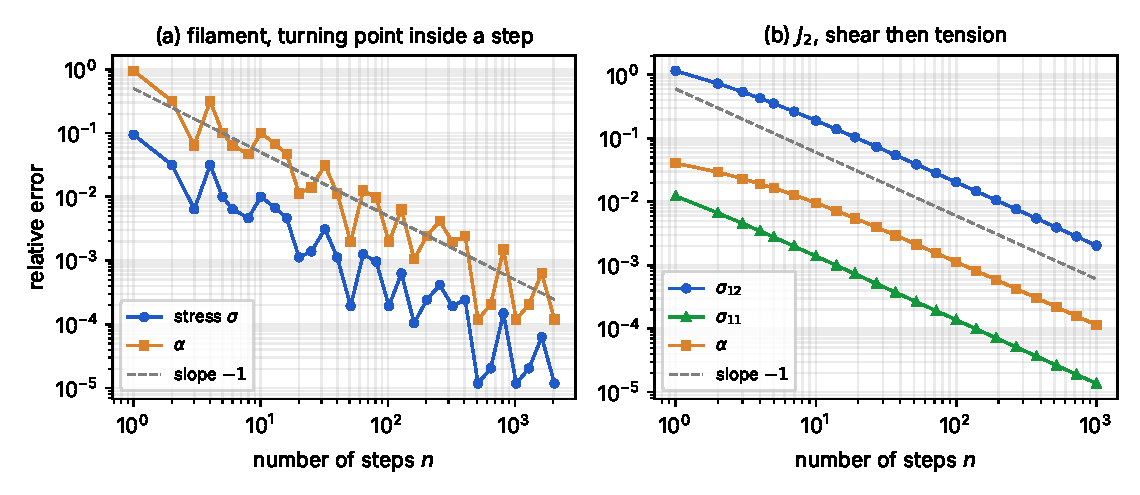
\includegraphics[width=\textwidth]{figures/ch5/errors.pdf}
\caption{Relative errors of the return map against the number of steps $n$.
(a) Filament of Exercise~\ref{exo:pn-nonmono}: the turning point of the
strain lies inside a step; the error decreases like $1/n$ on average, with
fluctuations due to the position of the turning point in its step.
(b) Shear then tension at fixed shear, Exercise~\ref{exo:pn-shear}: the
errors on $\sigma_{12}$, $\sigma_{11}$ and $\alpha$ are first order. The
dashed lines have the slope $-1$.}
\label{fig:pn-errors}
\end{figure}

\exercise{The plane-stress projected return}\label{exo:pn-ps}
\index{plane stress!exercise}%
(a) Show that $\mat{C}\mat{P}$ has the eigenvalues $E/(3(1-\nu))$, on
$(1,1,0)$, and $2\mu$, twice, and derive the decoupled update
\[
  \sigma_{11}+\sigma_{22}=\frac{(\sigma_{11}+\sigma_{22})^\trial}{1+\frac{E\dg}{3(1-\nu)}},\qquad
  (\sigma_{11}-\sigma_{22},\ \sigma_{12})=\frac{(\sigma_{11}-\sigma_{22},\ \sigma_{12})^\trial}{1+2\mu\dg},
\]
and the function $\varphi^2(\dg)$ of Box~5.5. (b) With $K=2$\,GPa, compute in
one step uniaxial tension to $\varepsilon_{11}=0.01$ and balanced biaxial
tension to $\varepsilon_{11}=\varepsilon_{22}=0.005$, and compare with the
closed forms. (c) Prescribe the in-plane strains: plane strain
($\varepsilon_{22}=0$) to $\varepsilon_{11}=0.01$. Is one step exact? The
script uses \texttt{plane\_stress\_return} (Box~5.5) of \texttt{ci\_core}.
\begin{solution}
(a) $\mat{C}$ and $\mat{P}$ commute and share the eigenvectors given in
Section~\ref{sec:pn-ps}; the products of their eigenvalues are
$\tfrac13E/(1-\nu)$, $2\mu$ and $2\mu$. In that basis
$(\mat{I}+\dg\mat{C}\mat{P})^{-1}$ is diagonal, which gives the update. Then
$\varphi^2=\vect{\sigma}\T\mat{P}\vect{\sigma}=\tfrac16(\sigma_{11}+\sigma_{22})^2+\tfrac12(\sigma_{11}-\sigma_{22})^2+2\sigma_{12}^2$.
(b) Uniaxial: $\alpha=\varepsilon^p_{11}$ and $\sigma=(\sY+K\varepsilon_{11})/(1+K/E)=267.326733$\,MPa;
biaxial: $\alpha=2\varepsilon^p_{11}$ and
$\sigma=(\sY+2K\varepsilon_{11})/(1+2K(1-\nu)/E)=266.272189$\,MPa. One step
gives both values to all digits: the stress direction is fixed by symmetry
($\sigma_{22}=0$, or $\sigma_{11}=\sigma_{22}$), and so is the normal.
(c) No. A proportional \emph{strain} path is not a proportional stress path:
the stress moves along the yield surface from the elastic ratio
$\sigma_{22}/\sigma_{11}=\nu$ towards the plane-strain value $\tfrac12$, as in
Exercise~\ref{exo:pl-sheet}. The one-step error is $6.9$\,MPa, and $0.22$,
$0.012$, $0.0010$\,MPa with 10, 100, 1000 steps. A code may reproduce the
tensile and bulge tests exactly at one step per increment and still need
small steps on a forming path.
\lstinputlisting[firstline=4]{python/examples/ch5/exo_plane_stress.py}
\end{solution}

\exercise{Hill anisotropy and the symmetry of the tangent}\label{exo:pn-hill}
\index{Hill criterion}\index{consistent tangent!symmetry}%
Hill's criterion~\cite{Hill1948} replaces the von Mises norm by
$\sigma_{eq}^2=\vect{\sigma}\cdot\mat{P}_H\vect{\sigma}$, with a symmetric positive
semi-definite matrix $\mat{P}_H$ that vanishes on hydrostatic stresses.
(a) Show that the backward Euler step with the associative flow
$\Delta\epsp=\dg\,\partial_{\sig}\sigma_{eq}$ is a closest-point projection, and
deduce that its consistent tangent is symmetric. (b) What happens if the flow
follows a different potential $g\ne\sigma_{eq}$ (for instance von Mises, while
the yield criterion is Hill's)? Check numerically by finite differences. The
script is self-contained: it does not use \texttt{ci\_core}, whose return maps
are written for von Mises and Tresca only.
\begin{solution}
(a) The projection property (Section~\ref{thm:pn-cpp}) holds for every convex $\Esig$: the elastic
domain of Hill's criterion is convex, and the step is the projection onto it.
By Section~\ref{thm:pn-W} the stress is the gradient of a convex potential
$W_n$, so its derivative is symmetric. In the linearization the rank-one term
is $(\bbC:\partial_{\sig}g)\otimes(\bbC:\partial_{\sig}f)/(\dots)$, symmetric
when $g=f$. (b) With $g\ne f$ the step is no longer a projection, there is no
potential, and the rank-one term is not symmetric. A general backward Euler
solver (Newton on $(\sig,\dg)$) and centred finite differences give, at a
generic strain, a relative asymmetry $\norm{\bbCalg-\bbCalg{}\T}/\norm{\bbCalg}$ of $10^{-9}$
(the finite-difference error) for von Mises and for associative Hill, and
$2.5\times10^{-2}$ for the non-associative model. The global stiffness is then
unsymmetric: a symmetric solver with the symmetrized tangent loses the
quadratic convergence, and the contractivity of
Section~\ref{thm:pn-contract} is lost.
\lstinputlisting[firstline=4]{python/examples/ch5/exo_hill.py}
\end{solution}

\framesub{Corners, stability and minimization}

\exercise{The Tresca corner}\label{exo:pn-tresca}
\index{Tresca criterion!corner (exercise)}%
In principal stresses take the two faces $f_a=\sigma_1-\sigma_3-\sY$ and
$f_b=\sigma_2-\sigma_3-\sY$, perfect plasticity, and Koiter's rule
$\Delta\epsp=\dg^a\tens N_a+\dg^b\tens N_b$. (a) Compute
$\tens N_i:\bbC:\tens N_j$ and the corner return. (b) Show that the corner is
the correct return if and only if $2f_b^\trial>f_a^\trial$, and interpret.
(c) With $\mu=76.92$\,GPa, sweep $f_b^\trial$ from $20$ to $5$\,MPa at
$f_a^\trial=20$\,MPa, with \texttt{tresca\_return} (Box~5.4) of
\texttt{ci\_core}.
\begin{solution}
(a) $\tens N_a=\ve_1\otimes\ve_1-\ve_3\otimes\ve_3$ and
$\tens N_b=\ve_2\otimes\ve_2-\ve_3\otimes\ve_3$ are deviatoric, so
$\bbC:\tens N_i=2\mu\tens N_i$, $\tens N_a:\bbC:\tens N_a=4\mu$ and
$\tens N_a:\bbC:\tens N_b=2\mu$. The two consistency conditions
$f_i^\trial-\sum_j\tens N_i:\bbC:\tens N_j\,\dg^j=0$ form a $2\times2$ system
of determinant $12\mu^2$, whose solution is in Box~5.4.
(b) The Kuhn--Tucker conditions require $\dg^b=(2f_b-f_a)/(6\mu)\ge0$ ($\dg^a\ge0$
holds since $f_a\ge f_b$). The trial state must lie in the cone of normals of
the vertex, where the closest point of $\Esig$ is the vertex itself. If
$\dg^b<0$, the face return applies, with $\dg^a=f_a/(4\mu)$.
(c) The corner is selected for $f_b=20$ ($\dg^a=\dg^b=4.33\times10^{-5}$) and $11$\,MPa
($\dg^b=4.3\times10^{-6}$); at $f_b=10$\,MPa, $\dg^b=0$, and below the face
return applies with $\dg^a=6.5\times10^{-5}$. The switch is continuous; the
tangent jumps. At the corner the plastic strain increment can be any positive
combination of $\tens N_a$ and $\tens N_b$ (Koiter's cone): the stress is
determined, the direction of flow depends on the trial state.
\lstinputlisting[firstline=4]{python/examples/ch5/exo_tresca.py}
\end{solution}

\exercise{Contractivity of the return map}\label{exo:pn-contract}
\index{B-stability!exercise}%
(a) Show that the return map never increases distances (Section~\ref{thm:pn-contract}) for perfect plasticity, where the
norm is $\norm{\sig}_E^2=\sig:\bbS:\sig$. (b) Show that forward Euler is not
contractive with the filament example of Section~\ref{sec:pn-stab}.
(c) Numerical test, perfect $J_2$ plasticity: state A is virgin; state B was
loaded plastically in tension ($\varepsilon_{11}=0.004$, lateral strains
$-0.002$) and brought back to zero strain. Both are then sheared to
$\gamma=0.03$ in $n$ steps. Follow the distance between the two stresses. The
script uses \texttt{radial\_return} of \texttt{ci\_core}, and a forward
Euler update written in the script.
\begin{solution}
(a) The trial stresses differ by $\sig_n-\sig'_n$, and the return map is the
projection onto $\Esig$ for $\scal{\cdot}{\cdot}_E$, which is non-expansive.
(b) With $\sigma=\sY$, $\sigma'=\sY-10$\,MPa and $\Delta\varepsilon=2.5\times10^{-4}$:
forward Euler gives $\sigma_\np=\sY$ and $\sigma'_\np=\sY+40$\,MPa, outside the
domain, and the distance grows from 10 to 40\,MPa; the return map gives
$\sigma_\np=\sigma'_\np=\sY$. (c) With backward Euler the distance decreases at
every step, for 4, 20 and 500 steps, from $0.52$ to $10^{-3}$, $7\times10^{-6}$
and $1.5\times10^{-7}$ (energy norm, $\sqrt{\mathrm{MPa}}$,
Figure~\ref{fig:pn-contract}): the two histories are forgotten, as plastic
flow forgets the initial state. Forward Euler leaves
the yield surface by up to $300\,\%$ with 4 steps and $2\,\%$ with 500 steps.
Contractivity is the discrete form of dissipation; a scheme without it can
create energy and is unstable in dynamics.
\lstinputlisting[firstline=4]{python/examples/ch5/exo_contract.py}
\end{solution}

\begin{figure}[h]
\centering
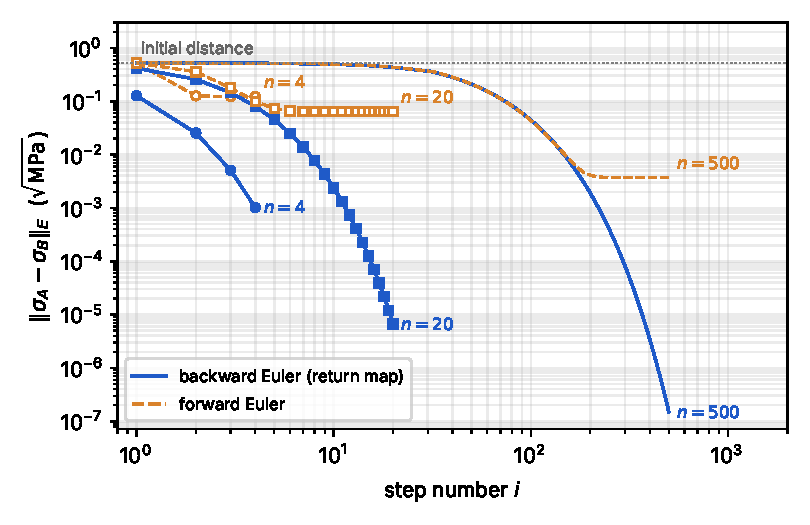
\includegraphics[width=0.66\textwidth]{figures/ch5/contract.pdf}
\caption{Exercise~\ref{exo:pn-contract}: energy distance between the stresses
of the virgin state A and of the pre-strained state B, both sheared to
$\gamma=0.03$ in $n=4$, $20$ and $500$ steps, against the step number (both
axes logarithmic). The return map (solid) decreases the distance at every
step, from $0.52\,\sqrt{\mathrm{MPa}}$ (dotted line) to zero. Forward Euler
(dashed) stalls at a distance that depends on the step size.}
\label{fig:pn-contract}
\end{figure}

\exercise{Viscoplastic updates as minimizations}\label{exo:pn-vp}
\index{viscoplasticity!exercise}%
(a) Show that the Perzyna step~\eqref{eq:pn-perzyna} is the minimizer of
$\displaystyle \tfrac12\norm{\vSig^\ast-\vSig^\trial}_E^2+\frac{\Delta t}{2\eta}\mac{f(\vSig^\ast)}^2$.
(b) For the filament without hardening, write the Perzyna and Duvaut--Lions
steps, and compare them with the exact relaxation~\eqref{eq:pl-relax} for a
strain held fixed after a jump.
\begin{solution}
(a) The function is strictly convex ($\mac{f}^2$ is convex for convex $f$).
Its stationarity condition is
$\tensf{G}^{-1}(\vSig-\vSig^\trial)+\frac{\Delta t}{\eta}\mac{f(\vSig)}\partial f(\vSig)=\vzero$,
i.e.\ $\vSig=\vSig^\trial-\tensf{G}\Delta\vz$ with
$\Delta\vz=\frac{\Delta t}{\eta}\mac{f}\partial f$: the backward Euler step. As
$\eta\to0$ the penalty forces $f\le0$ and the projection is recovered.
(b) Without hardening the two models coincide in one dimension ($\tau=\eta/E$).
For $\sigma^\trial>\sY$ both give
$\sigma_\np-\sY=(\sigma^\trial-\sY)/(1+\Delta t/\tau)$, while the exact
solution is $(\sigma^\trial_\np-\sY)e^{-\Delta t/\tau}$ after the jump. The ratio
$1/(1+r)$ approximates $e^{-r}$ to first order, and both tend to zero as
$r\to\infty$: the scheme is stable for every step and relaxes to the yield
surface.
\end{solution}

\exercise{Incremental potential of \texorpdfstring{$J_2$}{J2} plasticity}\label{exo:pn-W}
\index{incremental potential!exercise}%
(a) Derive~\eqref{eq:pn-WJ2} for combined linear hardening. (b) Show that its
gradient is $\sig_\np$ and its Hessian $\bbCalg$, and find the eigenvalues of
$\bbCalg$. (c) Deduce that $W_n$ is strongly convex if $K+H>0$.
\begin{solution}
(a) $\Delta\vz=\dg\,(\tn,\sqrt{2/3},\tn)$ for $(\epsp,\alpha,\valpha_{\mathrm{kin}})$,
$\tensf{G}=\diag(\bbC,K,\tfrac23H\bbI)$, so that
$\Delta\vz\cdot\tensf{G}\Delta\vz=\dg^2(2\mu+\tfrac23K+\tfrac23H)=h\dg^2=\mac{f^\trial}^2/h$;
insert in item (b) of Section~\ref{thm:pn-W}. (b) In the plastic region,
$\partial f^\trial/\partial\eps=2\mu\tn$ and
$\partial\tn/\partial\eps=\frac{2\mu}{\norm{\teta^\trial}}(\bbIdev-\tn\otimes\tn)$.
The gradient is $\sig^\trial-2\mu\frac{f^\trial}{h}\tn=\sig_\np$; differentiating
again gives~\eqref{eq:pn-calg}. The eigenvalues are $3\kappa$,
$2\mu(K+H)/(3\mu+K+H)$ and $2\mu\theta$ (multiplicity four).
(c) Since $f^\trial\le\norm{\teta^\trial}$, $\theta\ge1-2\mu/h=(K+H)/(3\mu+K+H)$:
all eigenvalues are bounded below by
$m=\min\{3\kappa,\,2\mu(K+H)/(3\mu+K+H)\}>0$, in the elastic region too.
The elastic region of $\eps$-space is convex, so a segment crosses its
boundary at most twice, and the gradient is strongly monotone along every
segment. Without hardening $m=0$ and the potential grows linearly.
\end{solution}

\framesub{A finite element code}

\exercise{The thick-walled cylinder by finite elements}\label{exo:pn-fem}
\index{thick-walled cylinder!finite elements}%
Write an axisymmetric plane-strain finite element code for the cylinder of
Exercise~\ref{exo:pl-cyl} (linear elements, unknown $u(r)$, strains
$(\dd u/\dd r,\ u/r,\ 0)$), with the radial return of Box~5.2 and the global
Newton method of Box~5.3 (Algorithm~\ref{alg:pn-fem}). For perfect plasticity,
$\sY=250$\,MPa, $b=2a$, apply $p=0.8\,p_L$ and $0.95\,p_L$ with
$\displaystyle p_L=\frac{2\sY}{\sqrt3}\ln\frac ba$, and compare the radius of the plastic
zone with the Tresca-type solution of Exercise~\ref{exo:pl-cyl}. The module
\texttt{ci\_fem} (page~\pageref{sec:pn-aux}) is such a code, built on
\texttt{radial\_return} of \texttt{ci\_core}; the test program below calls its
functions \texttt{solve} and \texttt{p\_of\_c}.
\begin{algorithm}[H]
\caption{Incremental Newton solver (Box~5.3)}\label{alg:pn-fem}
\begin{algorithmic}[1]
\Require mesh, material, load steps $p_1<\dots<p_N$, tolerance $\epsilon$
\Ensure nodal displacements $\mat{u}_n$, internal variables $\vz_n$ at the Gauss points
\State $\mat{u}\gets\mat{0}$;\ \ $\vz_0\gets\vzero$ at every Gauss point
\For{$n=0,\dots,N-1$}
  \Repeat
    \State $\mat{F}^{\mathrm{int}}\gets\mat{0}$;\ \ $\mat{K}\gets\mat{0}$
    \For{each element $e$ and Gauss point $g$}
      \State $(\sig,\vz^{\ast}_g,\bbCalg)\gets\textsc{RadialReturn}(\mat{B}_g\mat{u},\ \vz_{n,g})$ \Comment{from $\vz_n$}
      \State $\mat{F}^{\mathrm{int}}\mathrel{+}=w_g\mat{B}_g\T\sig$;\ \ $\mat{K}\mathrel{+}=w_g\mat{B}_g\T\mat{C}^{\mathrm{alg}}\mat{B}_g$
    \EndFor
    \State $\mat{R}\gets\mat{F}^{\mathrm{ext}}(p_\np)-\mat{F}^{\mathrm{int}}$
    \If{$\norm{\mat{R}}>\epsilon\norm{\mat{F}^{\mathrm{ext}}}$} \ $\mat{u}\gets\mat{u}+\mat{K}^{-1}\mat{R}$ \EndIf
  \Until{$\norm{\mat{R}}\le\epsilon\norm{\mat{F}^{\mathrm{ext}}}$}
  \State $\vz_{\np,g}\gets\vz^{\ast}_g$ at every Gauss point \Comment{accept the step}
\EndFor
\end{algorithmic}
\end{algorithm}
\begin{solution}
With 200 elements and 20 steps, $p_L=200.09$\,MPa. At $0.8\,p_L$ the plastic
zone reaches $c=131.0$\,mm against $130.8$\,mm, and at $0.95\,p_L$ $c=165.5$
against $164.0$\,mm. The small difference is not a discretization error: the
closed form assumes $\sigma_\theta-\sigma_r=2\sY/\sqrt3$, which is exact for
von Mises only when $\sigma_z$ is the mean of $\sigma_r$ and $\sigma_\theta$,
i.e.\ for incompressible plastic flow; in the elastic--plastic regime the
elastic compressibility makes $\sigma_z$ differ slightly. Near $p_L$ the bore
displacement grows quickly and Newton needs more iterations; at $p_L$ the
tangent stiffness becomes singular. The weight of a Gauss point is
$w_g=r_g\,L_e$ (the factor $2\pi$ cancels). Over the whole range from the
first yield, at $p=0.541\,p_L$, to $0.98\,p_L$, the computed radius follows
the closed form (Figure~\ref{fig:pn-cylzone}); the gap stays below $0.7$\,mm
up to $0.9\,p_L$ and grows to $2.6$\,mm at $0.98\,p_L$. Near $p_L$ the curve
$c(p)$ is steep, and a small difference in pressure, due to the
approximation on $\sigma_z$ discussed above, becomes a large difference in
radius.
Compare with similar computations performed in standard finite element codes,
for example Cast3M or FEniCS.
\lstinputlisting[firstline=90]{python/examples/ch5/ci_fem.py}
\end{solution}

\begin{figure}[h]
\centering
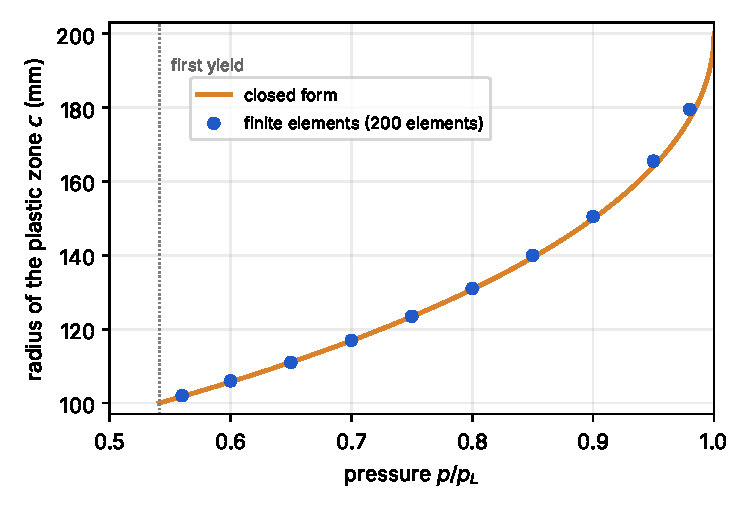
\includegraphics[width=0.6\textwidth]{figures/ch5/cylinder_zone.pdf}
\caption{Exercise~\ref{exo:pn-fem}: radius $c$ of the plastic zone of the
thick-walled cylinder ($b=2a=200$\,mm, perfect $J_2$ plasticity) against the
pressure. Finite elements (200 elements, 20 load steps per computation)
against the closed form
$p=k\ln(c/a)+\tfrac k2\bigl(1-c^2/b^2\bigr)$, $k=2\sY/\sqrt3$. The plastic
zone appears at $p=0.541\,p_L$ and reaches the outer radius at $p_L$.}
\label{fig:pn-cylzone}
\end{figure}

%======================================================================
\begin{chapterbib}{99}
\bibitem{BauschkeCombettes2017} H.~H.~Bauschke, P.~L.~Combettes, \emph{Convex Analysis and Monotone Operator Theory in Hilbert Spaces}, 2nd ed., Springer, 2017.
\bibitem{deSouzaNeto2008} E.~A.~de Souza Neto, D.~Peri\'c, D.~R.~J.~Owen, \emph{Computational Methods for Plasticity: Theory and Applications}, Wiley, 2008.
\bibitem{Hill1948} R.~Hill, A theory of the yielding and plastic flow of anisotropic metals, \emph{Proc. R. Soc. Lond. A} 193 (1948) 281--297.
\bibitem{KondoMaitournam2023b} D.~Kondo, H.~Maitournam, Thermodynamics of irreversible processes: formulation of constitutive models, Chapter~2 in J.~Besson et al., \emph{MEALOR II: Damage Mechanics and Local Approach to Fracture}, 2023, 5--38, doi:10.5281/zenodo.10125170.
\bibitem{KriegKey1976} R.~D.~Krieg, S.~W.~Key, Implementation of a time independent plasticity theory into structural computer programs, in J.~A.~Stricklin, K.~J.~Saczalski (eds.), \emph{Constitutive Equations in Viscoplasticity: Computational and Engineering Aspects}, AMD-20, ASME, 1976, 125--137.
\bibitem{KriegKrieg1977} R.~D.~Krieg, D.~B.~Krieg, Accuracies of numerical solution methods for the elastic--perfectly plastic model, \emph{J. Pressure Vessel Technol.} 99 (1977) 510--515.
\bibitem{Maitournam2012b} H.~Maitournam, \emph{Mat\'eriaux et structures an\'elastiques}, Presses de l'\'Ecole polytechnique, 2012.
\bibitem{Miehe2002} C.~Miehe, Strain-driven homogenization of inelastic microstructures and composites based on an incremental variational formulation, \emph{Int. J. Numer. Meth. Engng} 55 (2002) 1285--1322.
\bibitem{Moreau1965} J.-J.~Moreau, Proximit\'e et dualit\'e dans un espace hilbertien, \emph{Bull. Soc. Math. France} 93 (1965) 273--299.
\bibitem{OrtizPopov1985} M.~Ortiz, E.~P.~Popov, Accuracy and stability of integration algorithms for elastoplastic constitutive relations, \emph{Int. J. Numer. Meth. Engng} 21 (1985) 1561--1576.
\bibitem{OrtizSimo1986} M.~Ortiz, J.~C.~Simo, An analysis of a new class of integration algorithms for elastoplastic constitutive relations, \emph{Int. J. Numer. Meth. Engng} 23 (1986) 353--366.
\bibitem{OrtizStainier1999} M.~Ortiz, L.~Stainier, The variational formulation of viscoplastic constitutive updates, \emph{Comput. Methods Appl. Mech. Engrg.} 171 (1999) 419--444.
\bibitem{SimoGovindjee1991} J.~C.~Simo, S.~Govindjee, Non-linear B-stability and symmetry preserving return mapping algorithms for plasticity and viscoplasticity, \emph{Int. J. Numer. Meth. Engng} 31 (1991) 151--176.
\bibitem{SimoHughesCI} J.~C.~Simo, T.~J.~R.~Hughes, \emph{Computational Inelasticity}, Springer, 1998.
\bibitem{SimoKennedyGovindjee1988} J.~C.~Simo, J.~G.~Kennedy, S.~Govindjee, Non-smooth multisurface plasticity and viscoplasticity. Loading/unloading conditions and numerical algorithms, \emph{Int. J. Numer. Meth. Engng} 26 (1988) 2161--2185.
\bibitem{SimoTaylor1985} J.~C.~Simo, R.~L.~Taylor, Consistent tangent operators for rate-independent elastoplasticity, \emph{Comput. Methods Appl. Mech. Engrg.} 48 (1985) 101--118.
\bibitem{SimoTaylor1986} J.~C.~Simo, R.~L.~Taylor, A return mapping algorithm for plane stress elastoplasticity, \emph{Int. J. Numer. Meth. Engng} 22 (1986) 649--670.
\bibitem{Wilkins1964} M.~L.~Wilkins, Calculation of elastic-plastic flow, in B.~Alder, S.~Fernbach, M.~Rotenberg (eds.), \emph{Methods in Computational Physics}, Vol.~3, Academic Press, 1964, 211--263.
\end{chapterbib}

%======================================================================
\chapter{From prediction--correction to LATIN and the direct cyclic method}\label{ch:pl-cyc}
%======================================================================
% Sources: notes "Global-local methods for cyclic and monotone elastoplasticity"
% (2 Oct 2026); H. Maitournam, MEC562 "Mecanique des structures anelastiques"
% (2012), Sec. 3.6 (three-bar truss) and Ch. 4 (cyclic loads, vessel of
% Sec. 4.5); P. Ladeveze, Nonlinear Computational Structural Mechanics (1999),
% Ch. 3, 4, 7; Dang Van and Maitournam (1993); Maouche, Maitournam and
% Dang Van (1997); Maitournam, Pommier and Thomas (2002); MEALOR II Ch. 2.
% First draft (4 Oct 2026): Outline, Sections 6.1-6.3; Sections 6.4-6.8 are
% placeholders listing their content.

\framepart{Outline}
Chapter~\ref{ch:pl-num} computed an elastoplastic evolution step by step. In
every step a local problem, the return map at each Gauss point, alternates
with a global problem, equilibrium, until both are satisfied; then the next
step starts. This chapter keeps the two problems and changes the order in
which they are visited. The local stage is applied to a whole history at
each point, the global stage to all the instants of that history, and the
two alternate until the history converges. This is the idea of the
\emph{large time increment} (LATIN) method of
Ladev\`eze~\cite{LadevezeNCSM} and of the \emph{direct methods} of the
\'Ecole polytechnique for moving and cyclic
loads~\cite{DangVanMaitournam1993,MaoucheMaitournamDangVan1997,MaitournamPommierThomas2002}.
They compute the stabilized response of a structure under a cyclic or a
moving load without following the history cycle after cycle, which is what
fatigue design needs.

Two small structures are carried through the whole chapter. The three-bar
truss is a structure with one redundancy, loaded by forces: it shows how
plasticity redistributes the forces between the bars. The Bree vessel is a
wall loaded by a pressure and a cyclic temperature gradient: it shows
ratchetting. Each method of the chapter is computed on both, and the plots
show the computation itself, in time and in space, not only its result.

\paragraph{By the end of this chapter you should be able to:}
\begin{itemize}
  \item write the elastic solution, the residual stresses and the asymptotic
  regimes of the three-bar truss and of the Bree vessel;
  \item split an elastoplastic evolution into admissible and constitutive
  histories, and write the Melan decomposition of the solution;
  \item describe the incremental method and the iteration on the whole history
  as two orders of the same local and global computations, and say what each
  order guarantees;
  \item program the direct cyclic method, recognize its convergence, its
  non-convergence (ratchetting) and its non-unique limits;
  \item state the convergence theorem of the LATIN method, and explain the
  role of the search directions and of the relaxation;
  \item use Zarka's simplified analysis to estimate a shakedown state without
  following the history.
\end{itemize}

\paragraph{Plan of the chapter.} Section~\ref{sec:cy-models} presents the two
model problems and their asymptotic regimes. Section~\ref{sec:cy-split}
writes the evolution problem on a time window as the intersection of two sets
of histories. Section~\ref{sec:cy-orders} compares the two orders of
computation. Section~\ref{sec:cy-latin} treats the search directions and the
LATIN method, Section~\ref{sec:cy-period} the period map of cyclic loads,
Section~\ref{sec:cy-dcm} the direct cyclic and stationary methods, and
Section~\ref{sec:cy-zarka} Zarka's simplified analysis.
Section~\ref{sec:cy-map} places the other direct methods. A summary,
exercises with solutions (page~\pageref{sec:cy-exo}) and the references close
the chapter.

\begin{gbox}{Guiding questions}
\begin{enumerate}[itemsep=1pt]
  \item What does a structure become after many cycles of load, and how can
  this state be computed without following the cycles?
  (Sections~\ref{sec:cy-models}, \ref{sec:cy-period})
  \item Which equations are linear and global, which are nonlinear and local,
  and on which time window can they be split? (Section~\ref{sec:cy-split})
  \item Why does the step-by-step method always converge, and what can go wrong
  when the whole history is iterated at once? (Section~\ref{sec:cy-orders})
  \item Which search directions make the iteration on the whole history
  converge, and how fast? (Sections~\ref{sec:cy-latin}--\ref{sec:cy-zarka})
\end{enumerate}
The tools are the generalized standard materials and the uniqueness theorem of
Chapter~\ref{ch:pl}, the return map and its contractivity of
Chapter~\ref{ch:pl-num}, and the residual stresses and shakedown of
Example~\ref{ex:pl-bar}.
\end{gbox}

%======================================================================
\section{Two model problems}\label{sec:cy-models}
\index{model problems (cyclic plasticity)}%
Both structures are made of \emph{fibres} in uniaxial stress: the bars of the
truss, the layers of the wall. Each fibre $i$ has a strain $\varepsilon_i$, a
stress $\sigma_i$, a plastic strain $\varepsilon^p_i$ and the law of the
filament of Chapter~\ref{ch:pl-num} with linear kinematic hardening:
\begin{equation}\label{eq:cy-fibre}
  \sigma_i=E\,(\varepsilon_i-\varepsilon^p_i-\varepsilon^{th}_i),\qquad
  |\sigma_i-H\varepsilon^p_i|\le\sY,
\end{equation}
with the normality rule of Section~\ref{ssec:pl-1d-kin} and the back stress
$q_i=H\varepsilon^p_i$; $H=0$ is perfect plasticity and $\varepsilon^{th}_i$ a
thermal strain. The strains derive from a few nodal unknowns $\mat{u}$ and
the stresses balance the loads $\mat{F}(t)$:
\begin{equation}\label{eq:cy-discrete}
  \boldsymbol\varepsilon=\mat{B}\,\mat{u},\qquad
  \mat{B}\T\mat{W}\boldsymbol\sigma=\mat{F}(t),
\end{equation}
where $\mat{W}$ is the diagonal matrix of the fibre volumes. This is the
finite element structure of Section~\ref{sec:pn-incr} with one Gauss point per
fibre, small enough to be solved by hand and to be plotted completely.

\subsection{The three-bar truss}\label{ssec:cy-truss}
\index{three-bar truss}\index{residual stress!three-bar truss}%
The truss of Maitournam~\cite[Sec.~3.6]{Maitournam2012c} has three bars of
the same section $S$ and modulus $E$, hinged at the node $O$ and at the fixed
points $A$, $B$, $C$ (Figure~\ref{fig:cy-truss}). Bar~3 has the length $l$
and the direction $\vect e_1$; bars~1 and~2 have the length $l\sqrt2$ and
make angles of $\pm45^\circ$ with it. A force $\vect Q=Q_1\vect e_1+Q_2\vect
e_2$ acts at $O$. The bars carry the normal forces $N_i=S\sigma_i$, and the
elongation of bar $i$ is $\delta_i=\vect t_i\cdot\vect u$, where $\vect t_i$ is
its unit vector oriented towards $O$ and $\vect u$ the displacement of $O$.

\begin{figure}[h]
\centering
\begin{tikzpicture}[scale=1.25,>=Latex]
  \coordinate (O) at (0,0);
  \coordinate (A) at (-2,-2); \coordinate (B) at (-2,2); \coordinate (C) at (-2,0);
  \foreach \P in {A,B,C}{\fill[pattern=north east lines] ($(\P)+(-0.25,-0.22)$) rectangle ($(\P)+(0,0.22)$);
     \draw[thick] ($(\P)+(0,-0.22)$) -- ($(\P)+(0,0.22)$);}
  \draw[very thick,gray!70] (A) -- (O) node[midway,below right,black,font=\small] {1};
  \draw[very thick,gray!70] (B) -- (O) node[midway,above right,black,font=\small] {2};
  \draw[very thick,gray!70] (C) -- (O) node[midway,above,black,font=\small] {3};
  \foreach \P in {A,B,C,O}{\fill[white,draw=black] (\P) circle (1.5pt);}
  \node[left=6pt,font=\small] at (A) {$A$}; \node[left=6pt,font=\small] at (B) {$B$};
  \node[left=6pt,font=\small] at (C) {$C$}; \node[below right,font=\small] at (O) {$O$};
  \draw[->,very thick,orange!80!black] (O) -- (1.1,0) node[right] {$Q_1$};
  \draw[->,very thick,orange!80!black] (O) -- (0,1.1) node[above] {$Q_2$};
  \draw[|<->|] (-2,-2.45) -- (0,-2.45) node[midway,below,font=\small] {$l$};
  \draw[->] (0.6,-1.6) -- (1.1,-1.6) node[right,font=\small] {$\vect e_1$};
  \draw[->] (0.6,-1.6) -- (0.6,-1.1) node[above,font=\small] {$\vect e_2$};
\end{tikzpicture}
\caption{The three-bar truss of Maitournam~\cite{Maitournam2012c}: one degree of
redundancy, a force $(Q_1,Q_2)$ at the node $O$.}
\label{fig:cy-truss}
\end{figure}

\paragraph{Elastic solution.}
Equilibrium of $O$ gives two equations for three forces:
$N_2=N_1-\sqrt2\,Q_2$ and $N_3=Q_1+Q_2-\sqrt2\,N_1$. The truss is redundant of
degree one: the self-equilibrated forces form the line
\begin{equation}\label{eq:cy-truss-self}
  (N_1,N_2,N_3)=\gamma\,(1,1,-\sqrt2),\qquad \gamma\in\R .
\end{equation}
The elongations are compatible if they derive from a displacement of $O$,
that is, if they are orthogonal to the self-stresses:
$\delta_1+\delta_2=\sqrt2\,\delta_3$. With $\delta_i=N_il_i/(ES)$ this gives
$N_1+N_2=N_3$ and the elastic solution~\cite[eq.~(3.46)]{Maitournam2012c}
\begin{equation}\label{eq:cy-truss-el}
  N^{el}_1=\frac{Q_1}{2+\sqrt2}+\frac{Q_2}{\sqrt2},\qquad
  N^{el}_2=\frac{Q_1}{2+\sqrt2}-\frac{Q_2}{\sqrt2},\qquad
  N^{el}_3=\frac{2Q_1}{2+\sqrt2}.
\end{equation}
Under $Q_1$ alone, bar~3 yields first, at $Q_1=(2+\sqrt2)N_0/2\approx1.71N_0$
with $N_0=S\sY$, and the truss collapses at the limit load
$Q_L=(1+\sqrt2)N_0\approx2.41N_0$, when bars~1 and~2 yield as well.

\paragraph{Residual forces and the kernel.}
\index{Melan decomposition!three-bar truss}%
Let the bars carry plastic elongations $\delta^p_i=l_i\varepsilon^p_i$ at zero
load. The forces are self-equilibrated, hence of the
form~\eqref{eq:cy-truss-self}, and compatibility of the total elongations
$\delta_i=N_il_i/(ES)+\delta^p_i$ fixes $\gamma$:
\begin{equation}\label{eq:cy-truss-res}
  \gamma=-\frac{ES}{(4+2\sqrt2)\,l}\,\bigl(\delta^p_1+\delta^p_2-\sqrt2\,\delta^p_3\bigr).
\end{equation}
The residual forces see only the combination
$\delta^p_1+\delta^p_2-\sqrt2\,\delta^p_3$, the incompatibility of the plastic
elongations. A compatible plastic elongation, for instance $(a,-a,0)$, which
is the elongation produced by a vertical displacement of $O$, leaves no
residual force: it moves the node and nothing else.

\paragraph{Three loadings.}
Three periodic loadings of period $T=2\pi$ produce the three asymptotic
regimes of Section~\ref{sec:cy-period} (perfect plasticity,
Exercise~\ref{exo:cy-q-truss}):
\begin{itemize}
  \item $Q_1=1.1N_0(1-\cos t)$, $Q_2=0$: bar~3 yields in the first cycle, then
  the response is elastic. The range of $N^{el}_3$ is $1.29N_0<2N_0$; this is
  \emph{elastic shakedown}.
  \item $Q_1=1.9N_0\sin t$, $Q_2=0$: the range of $N^{el}_3$ is
  $2.23N_0>2N_0$. Bar~3 yields in tension and in compression in every cycle;
  this is \emph{alternating plasticity}.
  \item $Q_2=N_0$ constant and $Q_1=1.2N_0\sin t$: the constant force loads
  bars~1 and~2 with opposite signs, the alternating one with the same sign.
  Bar~1 yields in tension in one half-cycle, bar~2 in compression in the
  other, and the plastic elongations grow by $(a,-a,0)$ in every cycle, with
  $a=0.4\,\delta_Y$ ($\delta_Y=\sY l\sqrt2/E$): this is \emph{ratchetting}.
  The ratchet increment is compatible: it lies in the kernel of the
  residual-stress operator, and nothing in the stresses opposes it.
\end{itemize}
With kinematic hardening $H=0.05E$ the third loading no longer ratchets: the
plastic elongations converge, in about sixty cycles, to a state of elastic
shakedown. This slow approach is the test case of
Section~\ref{sec:cy-orders}.

\subsection{The Bree vessel}\label{ssec:cy-bree}
\index{Bree problem}\index{ratchetting!Bree problem}%
A thin vessel of mean radius $r_m$ and thickness $e$ contains a fluid at a
constant pressure, and its wall is crossed by a heat flux that is switched on
and off: the temperature varies linearly through the wall, with an amplitude
$\tau_0\lambda(t)$, $\lambda(t)=|\sin t|$. This is the problem of
Bree~\cite{Bree1967} for the fuel cans of fast reactors, in the form of the
spherical vessel of Maitournam~\cite[Sec.~4.5]{Maitournam2012c}. The only
stress is the hoop stress $\sigma(x,t)$, a function of the position
$x=(r-r_m)/e\in[-\tfrac12,\tfrac12]$ in the wall, and the hoop strain is the
same in all the layers:
\begin{equation}\label{eq:cy-bree}
  \sigma(x,t)=\tilde E\,\bigl(\varepsilon(t)-\varepsilon^p(x,t)+\alpha\tau_0x\lambda(t)\bigr),
  \qquad
  \int_{-1/2}^{1/2}\sigma(x,t)\dd x=\sigma_P ,
\end{equation}
where $\tilde E=E/(1-\nu)$ and $\sigma_P=p\,r_m/(2e)$ is the membrane stress
of the pressure. In the notation~\eqref{eq:cy-discrete}, the layers are the
fibres, $\mat{B}$ is a column of ones and $\mat{W}$ the layer thicknesses.

\paragraph{Elastic solution and residual stresses.}
Without plastic strain the mean of~\eqref{eq:cy-bree} gives
$\tilde E\varepsilon=\sigma_P$, hence
\begin{equation}\label{eq:cy-bree-el}
  \sigma^{el}(x,t)=\sigma_P+2\sigma_T\,x\,\lambda(t),\qquad
  \sigma_T=\tfrac12\tilde E\alpha\tau_0 :
\end{equation}
the outer skin is in tension and the inner skin in compression during
heating. With a plastic strain, the mean of~\eqref{eq:cy-bree} gives
$\varepsilon=\varepsilon^{el}+\langle\varepsilon^p\rangle$, where
$\langle\cdot\rangle$ is the mean through the wall, and
\begin{equation}\label{eq:cy-bree-melan}
  \sigma=\sigma^{el}+\rho,\qquad
  \rho(x,t)=-\tilde E\,\bigl(\varepsilon^p(x,t)-\langle\varepsilon^p\rangle(t)\bigr).
\end{equation}
The residual stress is the deviation of the plastic strain from its mean,
times $-\tilde E$. The mean itself, a uniform plastic strain, is compatible:
it changes the radius of the vessel and produces no stress. Ratchetting will
be a growth of $\langle\varepsilon^p\rangle$, invisible in the stresses.

\paragraph{The Bree diagram.}
\index{Bree diagram}%
With $X=\sigma_P/\sY$ and $Y=\sigma_T/\sY$, perfect plasticity, the
asymptotic regime depends only on $(X,Y)$ (Figure~\ref{fig:cy-bree-diagram}).
The response is elastic for $X+Y\le1$. It shakes down elastically for
$Y\le2$ and $X+Y/4\le1$, alternates for $Y>2$ and $XY\le1$, and ratchets
otherwise~\cite{Bree1967}; Maitournam~\cite[Sec.~4.5]{Maitournam2012c}
derives the ratchetting boundary $X+Y/4=1$ by following the first three
half-cycles. The figure is computed with the incremental method of
Chapter~\ref{ch:pl-num}, cycle after cycle, on a grid of $50\times60$ load
pairs; the computed regimes follow Bree's lines to the resolution of the
grid. The two cases marked (a) and (b) are used in
Sections~\ref{sec:cy-period}--\ref{sec:cy-dcm}.

\begin{figure}[h]
\centering
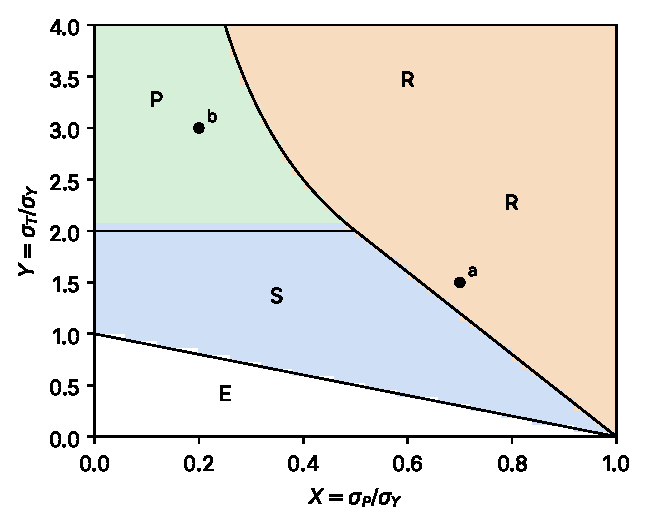
\includegraphics[width=0.5\textwidth]{figures/ch6/bree_diagram.pdf}
\caption{Bree diagram, perfect plasticity: elastic (E), elastic shakedown (S),
alternating plasticity (P) and ratchetting (R). Colours: regimes computed
cycle by cycle (30 cycles of 20 steps, 40 layers); lines: Bree's boundaries
$X+Y=1$, $Y=2$, $X+Y/4=1$, $XY=1$. Points (a) $X=0.7$, $Y=1.5$ and (b)
$X=0.2$, $Y=3$ are the cases of Sections~\ref{sec:cy-period}--\ref{sec:cy-dcm}.}
\label{fig:cy-bree-diagram}
\end{figure}

%======================================================================
\section{Two groups of equations on a time window}\label{sec:cy-split}
\index{global--local method}%
\subsection{Admissible and constitutive histories}
The quasi-static evolution problem of Chapter~\ref{ch:pl} (box in
Section~\ref{ssec:pl-bvp-eq}) splits into two groups of equations
(Figure~\ref{fig:pl-tonti}). Chapter~\ref{ch:pl-num} used the split at one
instant. Here it is used on a \emph{time window} $I$: one step $[t_n,t_\np]$,
the whole loading interval $[0,T]$, or one period. A \emph{history} on $I$ is
a set of fields $s=(\vu,\vz,\vSig)$ on $\Omega\times I$.
\begin{itemize}
  \item The \emph{admissible histories} $\Ad$ satisfy, at every instant of $I$,
  the kinematic conditions, equilibrium and the state laws
  $\sig=\bbC:(\eps[\vu]-\epsp)$, $\vq=-\bbD\valpha$, together with a
  \emph{closure} condition: the initial state $\vz(t_0)=\vz_0$, or the
  periodicity $\vz(t_0)=\vz(t_0+T)$. These equations are linear and global in
  space, and instantaneous in time: $\Ad$ is an affine set.
  \item The \emph{constitutive histories} $\Gcon$ satisfy the flow rule
  $\dot\vz\in N_{\Esig}(\vSig)$ at every point of $\Omega\times I$. These
  equations are nonlinear and local in space: each point carries its own
  evolution in time.
\end{itemize}
The solution is the history that belongs to both: $s\in\Ad\cap\Gcon$. Every
method of this chapter builds alternately a point of $\Ad$ (the \emph{global
stage}) and a point of $\Gcon$ (the \emph{local stage}).

\begin{proposition}[The two signs]\label{prop:cy-signs}
Let $s$, $s'$ be two histories on $I=[t_0,t]$ with the same closure data. If
$s,s'\in\Ad$, then
\[
  \int_{t_0}^{t}\!\!\int_\Omega(\vSig-\vSig')\cdot(\dot\vz-\dot\vz')\dd x\dd\tau
  =-\tfrac12\norm{(\vSig-\vSig')(t)}_E^2\le0
\]
when $\vSig(t_0)=\vSig'(t_0)$. If $s,s'\in\Gcon$, the same integral is
non-negative.
\end{proposition}
\begin{proof}
For admissible histories, the computation of the proof of
Theorem~\ref{thm:pl-unique} gives
$\displaystyle \frac{\dd}{\dd t}\tfrac12\norm{\Delta\vSig}_E^2=-\int_\Omega\Delta\vSig\cdot\Delta\dot\vz\dd x$,
because $\Delta\sig$ is self-equilibrated and $\Delta\dot\vu$ kinematically
admissible with zero data; integrate in time. For constitutive histories the
integrand is non-negative at every point by the monotonicity of the normal
cone (Corollary~\ref{cor:pl-monotone}).
\end{proof}
The uniqueness theorem of Chapter~\ref{ch:pl} is the case where $s$ and $s'$
are in both sets. The convergence proofs of
Section~\ref{sec:cy-latin} play the two signs against each other.

\subsection{The Melan decomposition}
\index{Melan decomposition}\index{residual stress!operator}%
The admissible set has an explicit structure. Let $(\vu^{el},\sig^{el})$ be the
\emph{fictitious elastic} response of the structure to the loads, the
response it would have without plasticity. For a plastic strain field $\epsp$
at zero load, let $\vw$ be the solution of the elastic problem with initial
strain $\epsp$:
\begin{equation}\label{eq:cy-eigen}
  \vw\in\Kad(\vzero,S_u),\qquad
  \int_\Omega\eps[\vw]:\bbC:\eps[\vv]\dd x=\int_\Omega\epsp:\bbC:\eps[\vv]\dd x
  \quad\forall\vv\in\Kad(\vzero,S_u),
\end{equation}
and define $\Pop\epsp=\eps[\vw]$ and $\Zop\epsp=\bbC:(\epsp-\Pop\epsp)$.
In finite elements, \eqref{eq:cy-eigen} is the system
$\mat{K}\mat{w}=\sum_e\int\mat{B}\T\mat{C}\,\epsp$ with the \emph{elastic}
stiffness, which is factorized once.

\begin{proposition}[Melan decomposition]\label{prop:cy-melan}
Every admissible history is of the form
\begin{equation}\label{eq:cy-melan}
  \eps=\eps^{el}+\Pop\epsp,\qquad
  \sig=\sig^{el}+\vrho,\qquad \vrho=-\Zop\epsp .
\end{equation}
The operator $\Pop$ is the projection onto the compatible strains, orthogonal
for the scalar product $\int_\Omega\vect a:\bbC:\vect b\dd x$. The residual
stress $\vrho$ is self-equilibrated; $\Zop$ is symmetric, positive
semi-definite, and its kernel is the set of compatible strains: a compatible
plastic strain produces no residual stress.
\end{proposition}
\begin{proof}
The problem is linear in the data $(\text{loads},\epsp)$; the elastic part
gives $\eps^{el}$, the plastic part gives $\Pop\epsp$ by~\eqref{eq:cy-eigen}.
By~\eqref{eq:cy-eigen}, $\vrho=\bbC:(\Pop\epsp-\epsp)$ satisfies
$\displaystyle \int_\Omega\vrho:\eps[\vv]\dd x=0$ for all admissible $\vv$; it is
self-equilibrated, and $\epsp-\Pop\epsp$ is orthogonal to the compatible strains.
If $\epsp=\eps[\vv]$ is compatible, $\Pop\epsp=\epsp$ and $\vrho=\vzero$.
\end{proof}
For the truss, $\Zop$ is the rank-one map~\eqref{eq:cy-truss-res}; for the
Bree vessel, $\Pop\varepsilon^p=\langle\varepsilon^p\rangle$ and
$\Zop\varepsilon^p=\tilde E(\varepsilon^p-\langle\varepsilon^p\rangle)$
by~\eqref{eq:cy-bree-melan}. In both cases the kernel of $\Zop$, the
compatible plastic strains, is the direction of ratchetting. Substituting the
decomposition~\eqref{eq:cy-melan} in the flow rule eliminates displacements
and equilibrium: the evolution problem becomes
\begin{equation}\label{eq:cy-reduced}
  \dot\vz\in N_{\Esig}\bigl(\sig^{el}(t)-\Zop\epsp,\ -\bbD\valpha\bigr),
  \qquad \text{closure on }\vz ,
\end{equation}
an evolution equation for the internal variables alone, local in time and
non-local in space through $\Zop$. It is a \emph{sweeping process} in the
sense of Moreau~\cite{Moreau1977}: the elastic domain, shifted by the elastic
stress $\sig^{el}(t)$, moves with the load and drags the internal variables.

\subsection{Three choices}
The methods of the chapter differ by three choices, which the rest of the
chapter takes one at a time.
\begin{gbox}{Window, closure, search directions}
\index{search directions}%
\begin{itemize}
  \item \textbf{Window} of one alternation of the local and global stages: one
  step (Chapter~\ref{ch:pl-num}), the interval $[0,T]$ (LATIN), one period
  (direct cyclic method), one streamline (stationary methods).
  \item \textbf{Closure}: initial state, periodicity $\vz(t_0)=\vz(t_0+T)$, or
  equality of the states upstream and downstream of a moving load.
  \item \textbf{Search directions}: the linear relations that link the point
  of $\Gcon$ to the previous point of $\Ad$ (local stage) and the next point of
  $\Ad$ to it (global stage): consistent tangent (Newton), elastic stiffness
  (initial strain), or a symmetric operator used in both stages (LATIN).
\end{itemize}
\end{gbox}

\begin{table}[h]
\centering\small
\renewcommand{\arraystretch}{1.15}
\begin{tabular}{@{}llll@{}}
\toprule
\sffamily method & \sffamily window & \sffamily closure & \sffamily global direction\\
\midrule
Newton (Box~5.3) & one step & initial & consistent tangent $\bbCalg$\\
initial strain (Box~6.1) & one step & initial & elastic $\bbC$\\
LATIN (Section~\ref{sec:cy-latin}) & $[0,T]$ & initial & symmetric $\mathbb L$, with relaxation\\
direct cyclic (Section~\ref{sec:cy-dcm}) & one period & periodic & elastic $\bbC$\\
stationary (Section~\ref{sec:cy-dcm}) & one streamline & upstream & elastic $\bbC$\\
\bottomrule
\end{tabular}
\caption{The methods of the chapter. In all of them the local stage is the
return map of Chapter~\ref{ch:pl-num} at fixed total strain, except LATIN,
whose local direction is $\mathbb L$.}
\label{tab:cy-methods}
\end{table}

\paragraph{A dictionary.}
The literature on these methods uses three notations. Ladev\`eze writes the
material in a ``normal formulation'' with internal variables $X$ and forces
$Y=AX$; Dang Van and Maitournam use internal parameters $a_k$ and forces
$A_k=Z:a_k$; Kondo and Maitournam~\cite{KondoMaitournam2023c} use the
irreversible forces $A=-\rho_0\,\partial\Psi/\partial(\cdot)$.
Table~\ref{tab:cy-dictionary} translates them into the notation of this book.
The only trap is a sign: Ladev\`eze's $Y$ and Dang Van--Maitournam's $A_k$ are
$-\vq$, while Kondo--Maitournam's force of a hardening variable is $\vq$.

\begin{table}[h]
\centering\small
\renewcommand{\arraystretch}{1.15}
\begin{tabular}{@{}llll@{}}
\toprule
 & \sffamily this book & \sffamily Ladev\`eze~\cite{LadevezeNCSM} & \sffamily Dang Van--Maitournam~\cite{DangVanMaitournam1993}\\
\midrule
Hooke, compliance & $\bbC$, $\bbS$ & $K$, $K^{-1}$ & $L$, $M$\\
hardening variables & $\valpha$ & $X$ & $a_k$\\
hardening law & $\vq=-\bbD\valpha$ & $Y=AX$ & $A_k=Z:a_k$\\
correspondence & & $X=\valpha$, $Y=-\vq$, $A=\bbD$ & $a_k=\valpha$, $A_k=-\vq$, $Z=\bbD$\\
dissipation & $\sig:\dot\eps^p+\vq\cdot\dot\valpha$ & $\sig:\dot\eps^p-Y\cdot\dot X$ & $\sig:\dot\eps^p-A_k\cdot\dot a_k$\\
flow rule & $\dot\vz\in\partial\varphi^\ast(\sig,\vq)$ & $(\dot\eps^p,-\dot X)=B(\sig,Y)$ & normality to $f(\sig,A_k)\le0$\\
admissible set & $\Ad$ & $A_d$ & KA, SA, state laws\\
constitutive set & $\Gcon$ & $\Gamma$ & integration along the path\\
\bottomrule
\end{tabular}
\caption{Notation of the LATIN method and of the direct methods in the
notation of this book (Table~\ref{tab:pl-dictionary}). In Kondo and
Maitournam~\cite[Sec.~2.6]{KondoMaitournam2023c}, with the plastic strain as
the kinematic variable, the force of $\epsp$ is $A_{\varepsilon^p}=\sig-\tbeta$
and the force of an isotropic variable is $q$.}
\label{tab:cy-dictionary}
\end{table}

%======================================================================
\section{Two orders for the same computations}\label{sec:cy-orders}
\index{direct method!order of the loops}\index{incremental method!order of the loops}%
\subsection{Step by step, or the whole history at once}
Discretize the window in instants $t_0<t_1<\dots<t_N$. Each method evaluates
the same two kinds of computations: a \emph{local} return map
$\vz_n=\mathcal R(\eps_n;\vz_{n-1})$ at each Gauss point and instant, and a
\emph{global} linear solve at each instant. They differ in the order of the
loops over the instants $n$ and over the iterations $k$
(Figure~\ref{fig:cy-orders}).

\providecommand{\cycorr}[2]{\draw[thick,#2,-{Latex[length=1.6mm]}] ($(#1)+(0.17,0.10)$)
   arc[start angle=-30,end angle=260,radius=0.2];}
\begin{figure}[h]
\centering
\begin{tikzpicture}[x=0.95cm,y=1cm,
  glob/.style={-{Latex[length=2mm]},thick,cphi},
  lab/.style={font=\small,align=left}]
  % (a) incremental
  \node[font=\sffamily\bfseries\small,right] at (-0.2,1.75) {(a) incremental};
  \draw[arr] (0,0) -- (9.6,0) node[right] {$t$};
  \foreach \x/\l in {0/t_0,3/t_{n-1},4.6/t_n,6.2/t_{n+1},9/t_N}
     {\draw (\x,0.1) -- (\x,-0.1) node[below] {$\l$};}
  \foreach \a/\b in {3/4.6,4.6/6.2}{
     \draw[glob,bend left=50] (\a,0.2) to (\b-0.05,0.35);
     \coordinate (c) at (\b,0.55); \cycorr{c}{cu}}
  \coordinate (c) at (3,0.55); \cycorr{c}{cu}
  \node[lab,cu] at (8.1,0.75) {$k=1,\dots,K_n$};
  % (b) direct
  \begin{scope}[yshift=-3.3cm]
  \node[font=\sffamily\bfseries\small,right] at (-0.2,2.25) {(b) whole history, iteration $k$};
  \draw[arr,gray] (0,0) -- (9.6,0) node[right,black] {$t$};
  \foreach \x in {0,1.25,2.5,3.75,5,6.25,7.5,8.75}{
     \draw[gray] (\x,0.08) -- (\x,-0.08);
     \draw[glob] (\x,1.55) -- (\x,1.05);
     \coordinate (c) at (\x,0.55); \cycorr{c}{cu}}
  \foreach \a/\b in {0/1.25,1.25/2.5,2.5/3.75,3.75/5,5/6.25,6.25/7.5,7.5/8.75}
     {\draw[cu,thick,-{Latex[length=1.6mm]}] (\a+0.22,0.67) to[bend left=35] (\b-0.2,0.67);}
  \draw[orange!80!black,thick,dashed,-{Latex[length=2mm]}] (8.75,-0.25) .. controls (8.6,-0.75) and (0.3,-0.75) .. (0,-0.25)
     node[pos=0.5,below,font=\scriptsize] {closure: $\vz(t_0)=\vz_0$, or $\vz(t_0)\gets\vz(t_N)$ (periodic)};
  \end{scope}
  % legend
  \begin{scope}[yshift=-5.0cm]
  \draw[glob] (0.1,0) -- (0.6,0); \node[lab,right] at (0.7,0) {global stage: equilibrium (elastic predictor)};
  \coordinate (c) at (0.35,-0.65); \cycorr{c}{cu}
  \node[lab,right] at (0.7,-0.6) {local stage: return map (plastic corrector), from $\vz(t_{n-1})$};
  \end{scope}
  % (c,d) lattice
  \begin{scope}[xshift=11.6cm,yshift=-0.4cm,x=0.5cm,y=0.42cm]
    \node[font=\sffamily\bfseries\small,right] at (-0.8,5.6) {(c) for $n$, for $k$};
    \foreach \i in {0,...,6}{\foreach \j in {0,...,3}{\fill[gray!60] (\i,\j) circle (1.4pt);}}
    \foreach \i in {0,...,5}{\draw[cu,thick,-{Latex[length=1.4mm]}] (\i,0.12) -- (\i,2.88);
       \draw[cphi,thick,-{Latex[length=1.4mm]}] (\i+0.08,3) .. controls (\i+0.5,3) and (\i+0.5,0) .. (\i+0.92,0);}
    \draw[cu,thick,-{Latex[length=1.4mm]}] (6,0.12) -- (6,2.88);
    \draw[->] (-0.5,-0.6) -- (6.6,-0.6) node[right,font=\scriptsize] {$n$};
    \draw[->] (-0.5,-0.6) -- (-0.5,3.6) node[above,font=\scriptsize] {$k$};
  \end{scope}
  \begin{scope}[xshift=11.6cm,yshift=-3.7cm,x=0.5cm,y=0.42cm]
    \node[font=\sffamily\bfseries\small,right] at (-0.8,5.6) {(d) for $k$, for $n$};
    \foreach \i in {0,...,6}{\foreach \j in {0,...,3}{\fill[gray!60] (\i,\j) circle (1.4pt);}}
    \foreach \j in {0,...,3}{\draw[cu,thick,-{Latex[length=1.4mm]}] (0.12,\j) -- (5.88,\j);}
    \foreach \j in {0,...,2}{\draw[cphi,thick,-{Latex[length=1.4mm]}] (5.95,\j+0.1) .. controls (3,\j+0.6) and (3,\j+0.4) .. (0.05,\j+0.9);}
    \draw[->] (-0.5,-0.6) -- (6.6,-0.6) node[right,font=\scriptsize] {$n$};
    \draw[->] (-0.5,-0.6) -- (-0.5,3.6) node[above,font=\scriptsize] {$k$};
  \end{scope}
\end{tikzpicture}
\caption{Two orders for the same computations. (a) Incremental: the elastic
predictor of the increment $t_{n-1}\to t_n$ (green) and the plastic corrector
(blue) are repeated at fixed $t_n$ until equilibrium; then the next step
starts. (b) Whole history: at iteration $k$ the global stage solves the
elastic problems of all the instants at once (they are independent), then
the local stage sweeps the history at each Gauss point, and the closure
condition starts the next iteration. (c), (d) The lattice of the computations
$(t_n,k)$, visited column by column or row by row.}
\label{fig:cy-orders}
\end{figure}

The incremental method of Chapter~\ref{ch:pl-num} loops \emph{for $n$, for
$k$}: it converges the equilibrium of $t_n$ before it looks at $t_\np$. The
iteration on the whole history loops \emph{for $k$, for $n$}: it visits all
the instants with the same (wrong) data, and corrects them all at the next
iteration. With the elastic stiffness in the global stage, the two
algorithms are written below; Box~6.1 is the modified
Newton method of Box~5.3.

\begin{gbox}{Box 6.1\quad Initial-strain iteration, step by step}
\index{initial-strain method}%
\begin{enumerate}[label=\textbf{\arabic*.},leftmargin=1.6em]
  \item \textbf{Step.} For $n=1,\dots,N$, start from $\mat{u}^{(0)}=\mat{u}_{n-1}$.
  \item \textbf{Local stage.} At each Gauss point,
  $(\sig^{(k)},\vz^{(k)})=\mathcal R(\mat{B}\mat{u}^{(k)};\vz_{n-1})$.
  \item \textbf{Global stage.} Solve
  $\mat{K}\,\delta\mat{u}=\mat{F}^{\mathrm{ext}}_n-\sum_e\int\mat{B}\T\sig^{(k)}$
  with the elastic stiffness $\mat{K}$, factorized once;
  $\mat{u}^{(k+1)}=\mat{u}^{(k)}+\delta\mat{u}$.
  \item \textbf{Test.} Repeat 2--3 until the residual is small; store
  $\vz_n=\vz^{(k)}$ and go to the next step.
\end{enumerate}
\end{gbox}

\begin{gbox}{Box 6.2\quad Iteration on the whole history}
\index{direct cyclic method!Box 6.2}%
\begin{enumerate}[label=\textbf{\arabic*.},leftmargin=1.6em]
  \item \textbf{Initialization.} $\epsp(t_n)=\vzero$ for all $n$ (or a guess);
  closure state $\vz(t_0)$.
  \item \textbf{Global stage.} For every instant $t_n$, solve the elastic problem
  with initial strain: $\mat{K}\mat{u}_n=\mat{F}^{\mathrm{ext}}_n+\sum_e\int\mat{B}\T\mat{C}\,\epsp(t_n)$
  (one factorization, $N$ independent solutions); $\eps_n=\mat{B}\mat{u}_n$.
  \item \textbf{Local stage.} At each Gauss point, sweep the history:
  $\vz(t_n)=\mathcal R(\eps_n;\vz(t_{n-1}))$, $n=1,\dots,N$.
  \item \textbf{Closure.} Initial condition: $\vz(t_0)=\vz_0$. Periodic
  (direct cyclic method): $\vz(t_0)\gets\vz(t_N)$.
  \item \textbf{Test.} Repeat 2--4 until the stresses of the two stages agree
  at all instants (and, if periodic, $\vz(t_N)=\vz(t_0)$).
\end{enumerate}
\end{gbox}

\subsection{What each order guarantees}
\paragraph{Why time stepping is the standard.}
The evolution problem~\eqref{eq:cy-reduced} with an initial condition is a
Cauchy problem, and it is causal: the state at $t$ depends on the past only.
The implicit Euler scheme for a sweeping process, Moreau's \emph{catching-up
algorithm}~\cite{Moreau1977}, is the return map; it is at the same time the
proof of existence of the solution and the algorithm that computes it. Each
step is the minimization of a strictly convex incremental potential
(Theorem~\ref{thm:pn-W}), with a unique solution and a globally convergent
Newton method; the next step starts from a converged state, close to the
solution; and the return map is contractive
(Theorem~\ref{thm:pn-contract}), so that an error made in a step is not
amplified by the following ones. Consistency and stability give the
convergence of the time discretization. Everything is local in time, and so
are the guarantees.

\paragraph{What the whole-history iteration risks.}
\index{ratchetting!non-convergence of direct methods}%
The iteration of Box~6.2 is a fixed-point iteration on
histories, $\epsp\gets\mathcal R_{[t_0,t_N]}(\eps^{el}+\Pop\epsp)$, and the
properties of each step do not transfer to it.
\begin{itemize}
  \item No theorem covers the pair ``return map at fixed total strain, elastic
  stiffness'' on a window. The LATIN theorem of Section~\ref{sec:cy-latin}
  needs other directions and a relaxation.
  \item Rate-independent plasticity has no fading memory. The return map is
  only non-expansive with respect to $\vz_{n-1}$, so that an error made at
  $t_n$ is carried unchanged to all later instants by the local sweep.
  Figure~\ref{fig:cy-truss-lattice}b shows it: a correction made at the first
  plastic instant reappears at every later instant, iteration after
  iteration, while the incremental method confines its iterations to the
  plastic steps.
  \item With the periodic closure, an error that is constant in time is not
  damped by the time coupling at all. In plasticity this is the kernel of
  $\Zop$: a compatible plastic strain added to a periodic state gives another
  periodic state. The iteration may converge to a periodic state that depends
  on its starting point, or not converge at all if the structure ratchets
  (Sections~\ref{sec:cy-period}--\ref{sec:cy-dcm}).
  \item The iterates are not states of any loading history; there is no energy
  that decreases from one iteration to the next unless the directions are
  chosen for it, as in LATIN.
\end{itemize}

\begin{figure}[h]
\centering
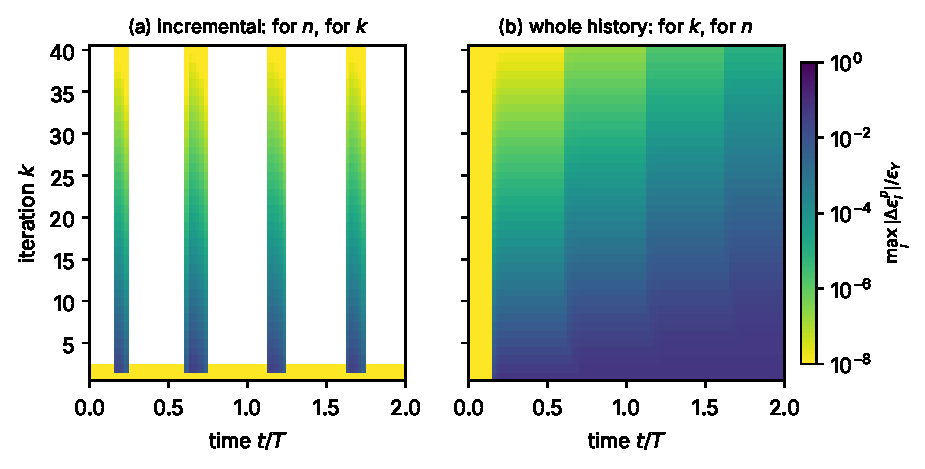
\includegraphics[width=0.85\textwidth]{figures/ch6/truss_lattice.pdf}
\caption{The lattice of Figure~\ref{fig:cy-orders} computed for the truss
($H=0.05E$, $Q_2=N_0$, $Q_1=1.2N_0\sin t$, two periods of 40 steps): size of the
plastic correction $\max_i|\Delta\varepsilon^p_i|$ at each instant $t_n$ and
iteration $k$. (a) Incremental initial-strain iteration (Box~6.1):
2 iterations at the elastic steps, up to 46 at the plastic ones, 982 local
evaluations in all. (b) Iteration on the whole history
(Box~6.2, initial condition): the corrections made at the
first plastic instants are carried to the end of the window; 40 iterations
($3200$ local evaluations) reach an indicator of $3\times10^{-6}$.}
\label{fig:cy-truss-lattice}
\end{figure}

\paragraph{When it pays.}
The whole-history iteration wins when its strengths matter more than its
risks:
\begin{itemize}
  \item \emph{Confined plasticity.} By~\eqref{eq:cy-melan}, the elastic
  prediction is exact outside the plastic zone, and the correction couples
  the plastic points only through $\Zop$ restricted to the plastic zone. A
  small plastic zone in an elastic structure (contact, notches, the skin of a
  thermal shock) gives a fast contraction.
  \item \emph{One loop instead of two.} Cycle after cycle, the incremental
  method converges the equilibrium of every step of every transient cycle,
  which is then thrown away. The direct cyclic method converges the
  equilibrium and the periodicity together.
  \item \emph{Cheap iterations.} The global stage uses the elastic stiffness,
  factorized once; the instants are independent and can be compressed in a
  Fourier or wavelet basis in time~\cite{MaitournamPommierThomas2002}; the
  local stage is parallel in space.
\end{itemize}
Figure~\ref{fig:cy-truss-process} compares the costs on the truss. For three
bars, factorizing the tangent is free, and the cycle-by-cycle computation
needs fewer local evaluations than the direct cyclic method (3750 against
13\,200 to reach $10^{-6}\varepsilon_Y$); Anderson acceleration of the period
map (Section~\ref{sec:cy-period}) needs four cycles. In a finite element model
the balance changes: the incremental method refactorizes the tangent at
every Newton iteration, the direct cyclic method never does, and Maouche et
al.~\cite{MaoucheMaitournamDangVan1997} report a computation of fretting
contact ten times faster in gross slip (3\,h against 30\,h for 74 cycles) and
twice as fast in partial slip.

\begin{figure}[h]
\centering
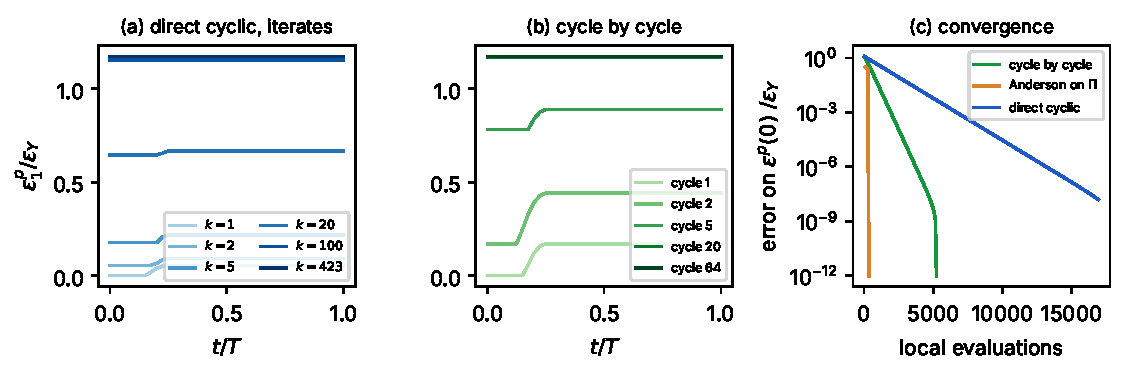
\includegraphics[width=\textwidth]{figures/ch6/truss_process.pdf}
\caption{Truss, $H=0.05E$, $Q_2=N_0$, $Q_1=1.2N_0\sin t$, one period of 40 steps.
(a) Plastic strain of bar~1 over the period, iterates $k$ of the direct cyclic
method (Box~6.2, periodic closure). (b) The same quantity in
cycles 1 to 64 of the incremental computation. (c) Error on the periodic
state against the number of local evaluations: cycle by cycle (Newton,
Box~5.3), Anderson acceleration of the period map, direct cyclic method.}
\label{fig:cy-truss-process}
\end{figure}

%======================================================================
\section{Search directions and the LATIN method}\label{sec:cy-latin}
\index{LATIN method}\index{large time increment method|see{LATIN method}}%
\draftnote{To be written. Content: Ladev\`eze's two-direction framework for one
step (Ch.~3 of~\cite{LadevezeNCSM}): local direction ``vertical'' (total strain
fixed) = return map; global direction tangent (Newton) or elastic (initial
strain, Nguyen 1977); convergence factor $E/(E+C)$ of the filament. LATIN on
$[0,T]$: directions on the rates, local stage with $\mathbb L$, global stage
Maxwell-type marched in time; theorem 4.1 of~\cite{LadevezeNCSM} with the
relaxation $\mu>0$, partial convergence for $\mu=0$ in statics (Thm.~4.3);
computation on the truss: with $\mu=0$ the indicator stalls although the
constitutive iterate is exact, with $\mu=0.3$ it converges (cy\_core.latin).
Radial (PGD) approximation and wavelets (Comte et al.) in one paragraph.}

%======================================================================
\section{Cyclic loads: the period map}\label{sec:cy-period}
\index{period map}\index{shakedown!period map}%
\draftnote{To be written. Content: adaptation, accommodation, rochet (Maitournam
Ch.~4); Halphen's results; contraction of distances (Proposition~\ref{prop:cy-signs});
period map non-expansive for the seminorm $\int\epsp:\Zop\epsp+\valpha\cdot\bbD\valpha$;
Picard, Krasnoselskii--Mann, Anderson; Bree case (a) with $H=0.02E$: 261 cycles,
Anderson 13; non-uniqueness: case (b), two exact periodic states differing by a
constant residual stress of $0.3\sigma_0$ (figure bree\_nonunique); local shakedown
theorem for linear kinematic hardening (Maitournam Sec.~4.4.3).}

%======================================================================
\section{The direct cyclic and stationary methods}\label{sec:cy-dcm}
\index{direct cyclic method}\index{stationary method}%
\draftnote{To be written. Content: Box~6.2 with periodic closure
(Akel--Nguyen; Maouche et al.\ 1997); Fourier in time (Maitournam, Pommier,
Thomas 2002); figures bree\_process (iterates in space at $T/2$) and
bree\_ratchet (drift of $\langle\varepsilon^p\rangle$, $0.060\varepsilon_Y$ per
iteration, residual stress converged to $10^{-15}$). Stationary methods
(Dang Van--Maitournam 1993): moving frame, PPSM, DSM, uniqueness; Cast3M
procedure @STATIO.}

%======================================================================
\section{Zarka's simplified analysis}\label{sec:cy-zarka}
\index{Zarka's method}%
\draftnote{To be written. Content: transformed parameter $Y=H\epsp-\vrho$; local
criterion centred on $\sig^{el}(t)$; elastic shakedown iff the intervals
(balls) intersect (Mandel--Halphen--Zarka 1977); projection of the state after
the first half-cycle; linear problem $(H\,\mathbb I+\Zop)\epsp=Y$; exact on the
truss and on Bree case S (cy\_core.zarka); Amiable et al.\ 2006; Cast3M @ZACPLUS.}

%======================================================================
\section{A map of the direct methods}\label{sec:cy-map}
\draftnote{To be written: one table (linear matching, residual stress
decomposition, optimal control of Peigney--Stolz, cycle jump, multi-time-scale
LATIN, PGD, Brezis--Ekeland--Nayroles), each with one line and one reference.}

%======================================================================
\framepart{Summary}
\begin{gbox*}
\begin{itemize}
  \item \textbf{Two model problems}: the three-bar truss (one redundancy,
  self-stresses $\gamma(1,1,-\sqrt2)$, limit load $(1+\sqrt2)N_0$) and the Bree
  vessel (residual stress $-\tilde E(\varepsilon^p-\langle\varepsilon^p\rangle)$,
  Bree diagram). Both show elastic shakedown, alternating plasticity and
  ratchetting.
  \item \textbf{Two groups of equations}: admissible histories $\Ad$ (linear,
  global, with a closure condition) and constitutive histories $\Gcon$
  (nonlinear, local); the solution is $\Ad\cap\Gcon$. On $\Ad$ the dissipation
  of a difference is non-positive, on $\Gcon$ non-negative.
  \item \textbf{Melan}: $\eps=\eps^{el}+\Pop\epsp$, $\sig=\sig^{el}-\Zop\epsp$;
  compatible plastic strains, the kernel of $\Zop$, give no residual stress and
  are the direction of ratchetting.
  \item \textbf{Two orders}: incremental (for $n$, for $k$) inherits the
  guarantees of each step; the iteration on the whole history (for $k$, for
  $n$) has none in general, carries errors forward without damping, and with a
  periodic closure may converge to non-unique states or drift. It pays when
  plasticity is confined, when many transient cycles are avoided, and when
  factorizations are expensive.
\end{itemize}
\draftnote{Summary of Sections 6.4--6.8 to be added.}
\end{gbox*}

\framepart{Exercises}\label{sec:cy-exo}
The computational exercises use the module \texttt{cy\_core}, which contains the
two model problems, the return map with a search direction, the global stage,
the incremental and whole-history solvers, the period map and Zarka's
estimate.\draftnote{Problems with code to be added with Sections 6.4--6.8.}

\framesub{Short questions}

\exercise{Regimes of the three-bar truss}\label{exo:cy-q-truss}
\index{three-bar truss!exercise}%
Elastic--perfectly plastic bars, $N_0=S\sY$. Using~\eqref{eq:cy-truss-el} and
Melan's theorem, find the regime under (a) $Q_1=1.1N_0(1-\cos t)$, $Q_2=0$;
(b) $Q_1=1.9N_0\sin t$, $Q_2=0$. (c) Under $Q_2=N_0$ and $Q_1=1.2N_0\sin t$,
show that the plastic elongation $(a,-a,0)$ is compatible, and explain why it
can grow without bound.
\begin{solution}
(a) $N^{el}_3=2Q_1/(2+\sqrt2)$ varies in $[0,\,1.289N_0]$ and $N^{el}_{1,2}$ in
$[0,\,0.644N_0]$. The constant residual field $\gamma(1,1,-\sqrt2)$ with
$\gamma=0.25N_0$ gives $N_3\in[-0.354,\,0.935]N_0$ and
$N_{1,2}\in[0.25,\,0.894]N_0$, inside $[-N_0,N_0]$: elastic shakedown (Melan).
Bar~3 yields in the first cycle since $\max N^{el}_3>N_0$. (b) The range of
$N^{el}_3$ is $4\times1.9/(2+\sqrt2)\,N_0=2.23N_0>2N_0$; no residual field can
bring it into $[-N_0,N_0]$: bar~3 yields in every cycle, alternating
plasticity. (c) $\delta^p_1+\delta^p_2-\sqrt2\,\delta^p_3=0$, so
by~\eqref{eq:cy-truss-res} the residual forces vanish: the increment is the
elongation of a vertical displacement of $O$. Nothing in the stresses
resists it; the computation gives $a=0.4\,\delta_Y$ per cycle.
\end{solution}

\exercise{Melan decomposition of the Bree vessel}\label{exo:cy-q-bree}
\index{Bree problem!exercise}%
From~\eqref{eq:cy-bree}, derive~\eqref{eq:cy-bree-melan}. Show that
$\Pop\varepsilon^p=\langle\varepsilon^p\rangle$ and that the kernel of $\Zop$ is
the set of uniform plastic strains. What does a uniform plastic strain mean
for the vessel?
\begin{solution}
Take the mean of~\eqref{eq:cy-bree} through the wall: $\langle x\rangle=0$, so
$\sigma_P=\tilde E(\varepsilon-\langle\varepsilon^p\rangle)$ and
$\varepsilon=\sigma_P/\tilde E+\langle\varepsilon^p\rangle$; substituting,
$\sigma=\sigma^{el}-\tilde E(\varepsilon^p-\langle\varepsilon^p\rangle)$. The
compatible strains are the uniform ones ($\mat{B}$ is a column of ones), and
$\Pop$ is the orthogonal projection on them, the mean. $\Zop\varepsilon^p=0$
if and only if $\varepsilon^p$ equals its mean. A uniform hoop plastic strain
is a permanent increase of the radius: the vessel swells without stress. It
is the ratchet strain of the Bree problem.
\end{solution}

\begin{chapterbib}{99}
\bibitem{Bree1967} J.~Bree, Elastic-plastic behaviour of thin tubes subjected to internal pressure and intermittent high-heat fluxes with application to fast-nuclear-reactor fuel elements, \emph{J. Strain Anal.} 2 (1967) 226--238.
\bibitem{DangVanMaitournam1993} K.~Dang Van, M.~H.~Maitournam, Steady-state flow in classical elastoplasticity: applications to repeated rolling and sliding contact, \emph{J. Mech. Phys. Solids} 41 (1993) 1691--1710.
\bibitem{KondoMaitournam2023c} D.~Kondo, H.~Maitournam, Thermodynamics of irreversible processes: formulation of constitutive models, Chapter~2 in J.~Besson et al., \emph{MEALOR II: Damage Mechanics and Local Approach to Fracture}, 2023, 5--38.
\bibitem{LadevezeNCSM} P.~Ladev\`eze, \emph{Nonlinear Computational Structural Mechanics: New Approaches and Non-Incremental Methods of Calculation}, Springer, 1999.
\bibitem{Maitournam2012c} H.~Maitournam, \emph{M\'ecanique des structures an\'elastiques: comportement, chargements cycliques et fatigue}, course notes MEC562, \'Ecole polytechnique, 2012.
\bibitem{MaitournamPommierThomas2002} M.~H.~Maitournam, B.~Pommier, J.-J.~Thomas, D\'etermination de la r\'eponse asymptotique d'une structure an\'elastique sous chargement thermom\'ecanique cyclique, \emph{C. R. M\'ecanique} 330 (2002) 703--708.
\bibitem{MaoucheMaitournamDangVan1997} N.~Maouche, M.~H.~Maitournam, K.~Dang Van, On a new method of evaluation of the inelastic state due to moving contacts, \emph{Wear} 203--204 (1997) 139--147.
\bibitem{Moreau1977} J.-J.~Moreau, Evolution problem associated with a moving convex set in a Hilbert space, \emph{J. Differential Equations} 26 (1977) 347--374.
\end{chapterbib}


\appendix
%======================================================================
\chapter{Prerequisites: tensor algebra and continuum mechanics}\label{app:prereq}
%======================================================================
% Added after the review of Oct 2026: "a short prerequisites appendix on
% tensor algebra and continuum mechanics".

\framepart{Outline}
This appendix recalls, in a few pages, the tensor algebra and the small-strain
continuum mechanics used throughout the book. It fixes the notation of the
list on page~\pageref{front:notation} and gives each operation in
Cartesian components. Section~\ref{sec:pre-tensors} treats vectors and
tensors, Section~\ref{sec:pre-calculus} the differential operators, and
Section~\ref{sec:pre-continuum} the kinematics, stresses and equilibrium of a
deformable body. Standard references are~\cite{SalenconPre,GurtinPre,ChadwickPre}.

%======================================================================
\section{Vectors and tensors}\label{sec:pre-tensors}
\index{tensor algebra}%
\paragraph{Components.} In an orthonormal basis $(\ve_1,\ve_2,\ve_3)$ a vector is
$\vu=u_i\ve_i$ and a second-order tensor $\tens{a}=a_{ij}\,\ve_i\otimes\ve_j$, with
summation over repeated indices. A second-order tensor is a linear map of
vectors: $(\tens{a}\vv)_i=a_{ij}v_j$. A fourth-order tensor
$\bbC=C_{ijkl}\,\ve_i\otimes\ve_j\otimes\ve_k\otimes\ve_l$ is a linear map of
second-order tensors: $(\bbC:\eps)_{ij}=C_{ijkl}\varepsilon_{kl}$.

\begin{gbox}{Products and contractions}
\begin{itemize}
  \item scalar product $\vu\cdot\vv=u_iv_i$; \ tensor product
  $(\vu\otimes\vv)_{ij}=u_iv_j$, so that $(\vu\otimes\vv)\vw=(\vv\cdot\vw)\,\vu$;
  \item double contraction $\tens{a}:\tens{b}=a_{ij}b_{ij}=\tr(\tens{a}\T\tens{b})$;
  \item transpose $(\tens{a}\T)_{ij}=a_{ji}$; symmetric part
  $\sym\tens{a}=\tfrac12(\tens{a}+\tens{a}\T)$; skew part $\tfrac12(\tens{a}-\tens{a}\T)$;
  \item trace $\tr\tens{a}=a_{ii}=\tI:\tens{a}$; deviator
  $\dev\tens{a}=\tens{a}-\tfrac13(\tr\tens{a})\tI$, with $\tr\dev\tens{a}=0$.
\end{itemize}
\end{gbox}

\paragraph{Orthogonal decompositions.} A symmetric tensor and a skew tensor
are orthogonal for ``$:$''; so are a spherical tensor $c\tI$ and a deviator.
Hence, for symmetric $\tens{a}$,
\[
  \tens{a}:\tens{a}=\tfrac13(\tr\tens{a})^2+\dev\tens{a}:\dev\tens{a},
\]
the identity behind the split of the elastic energy into a volume and a
shape part (Exercise~\ref{exo:posdef}) and behind the von Mises criterion.

\paragraph{Fourth-order identities.}
\index{identity tensor}%
On symmetric tensors, $\bbI$ with
$I_{ijkl}=\tfrac12(\delta_{ik}\delta_{jl}+\delta_{il}\delta_{jk})$ is the identity,
$\tfrac13\tI\otimes\tI$ the projector on spherical tensors and
$\bbIdev=\bbI-\tfrac13\tI\otimes\tI$ the projector on deviators. They are
orthogonal projectors: $\bbIdev:\bbIdev=\bbIdev$, $\bbIdev:(\tI\otimes\tI)=0$.
An isotropic tensor $\bbC=3K\,\tfrac13\tI\otimes\tI+2\mu\,\bbIdev$ is therefore
inverted by inverting its two eigenvalues: $\bbC^{-1}=\frac{1}{3K}\,\tfrac13\tI\otimes\tI+\frac{1}{2\mu}\,\bbIdev$.

\paragraph{Voigt notation.}
\index{Voigt notation}%
A symmetric second-order tensor has six independent components, and a
fourth-order tensor with the symmetries of elasticity has $21$. They are
stored as a column of six and a symmetric $6\times6$ matrix, with the index
pairs $11,22,33,23,31,12\mapsto1,\dots,6$: $\sigma_I=c_{IJ}\varepsilon_J$ with
the engineering shears $\varepsilon_4=2\varepsilon_{23}$, $\varepsilon_5=2\varepsilon_{31}$,
$\varepsilon_6=2\varepsilon_{12}$. The factor $2$ keeps the energy
$\tfrac12\sig:\eps=\tfrac12\sigma_I\varepsilon_I$. This is the notation of the
tables of moduli of Chapter~\ref{ch:elliptic}, equation~\eqref{eq:voigt}, and of
finite element codes; the Mandel variant, with factors $\sqrt2$, is discussed there.

\paragraph{Eigenvalues and invariants.} A symmetric tensor has three real
eigenvalues and an orthonormal eigenbasis (principal axes). Its principal
invariants are $I_1=\tr\tens{a}$, $I_2=\tfrac12\bigl((\tr\tens{a})^2-\tr\tens{a}^2\bigr)$
and $I_3=\det\tens{a}$; for a deviator one uses $J_2=\tfrac12\dev\tens{a}:\dev\tens{a}$
and $J_3=\det\dev\tens{a}$, the variables of isotropic yield criteria.

%======================================================================
\section{Differential operators}\label{sec:pre-calculus}
\index{gradient}\index{divergence}%
With $(\cdot)_{,j}=\partial(\cdot)/\partial x_j$:
\begin{gbox}{Gradient and divergence in Cartesian components}
\[
  (\nabla u)_i=u_{,i},\qquad (\nabla\vu)_{ij}=u_{i,j},\qquad
  \dive\vu=u_{i,i}=\tr\nabla\vu,\qquad (\dive\tens{a})_i=a_{ij,j},
\]
\[
  \Delta u=\dive\nabla u=u_{,ii},\qquad
  \dive(\tens{a}\T\vv)=(\dive\tens{a})\cdot\vv+\tens{a}:\nabla\vv .
\]
\end{gbox}
The last identity, integrated with the divergence theorem, is the integration
by parts of Theorem~\ref{thm:ibp-tensor}. In cylindrical or spherical
coordinates the components of $\nabla$ and $\dive$ contain extra terms from the
derivatives of the basis vectors; they are tabulated in~\cite{SalenconPre}.

%======================================================================
\section{Small-strain continuum mechanics}\label{sec:pre-continuum}
\paragraph{Kinematics.}
\index{strain}\index{compatibility}%
A body occupies $\Omega$; its points move by the displacement $\vu(\vx)$. When
the gradient is small, $|\nabla\vu|\ll1$, the change of length and angle is
measured by the small-strain tensor
\[
  \eps[\vu]=\tfrac12(\nabla\vu+\nabla\vu\T),\qquad
  \varepsilon_{ij}=\tfrac12(u_{i,j}+u_{j,i}).
\]
$\varepsilon_{11}$ is the relative elongation of a fibre along $\ve_1$,
$2\varepsilon_{12}$ the decrease of the right angle between $\ve_1$ and $\ve_2$,
and $\tr\eps$ the relative change of volume. The skew part of $\nabla\vu$ is an
infinitesimal rotation, and $\eps[\vu]=\vzero$ exactly for the rigid
displacements $\vu=\vect{a}+\vect{b}\times\vx$. Conversely, a symmetric field $\eps$
derives from a displacement in a simply connected domain if and only if it
satisfies the compatibility conditions
$\varepsilon_{ij,kl}+\varepsilon_{kl,ij}-\varepsilon_{ik,jl}-\varepsilon_{jl,ik}=0$.

\paragraph{Stresses.}
\index{stress}\index{Cauchy theorem}%
The force per unit area exerted across a surface element of normal $\vn$ is
the traction $\vt$. Cauchy's theorem states that it is linear in $\vn$:
$\vt=\sig\vn$, $t_i=\sigma_{ij}n_j$, with $\sig$ the Cauchy stress tensor. The
balance of moments makes $\sig$ symmetric. Its normal component
$\vn\cdot\sig\vn$ is the normal stress (positive in tension) and its
tangential part the shear stress.

\begin{gbox}{Equilibrium}
\index{equilibrium!local}%
For a body under body forces $\vf$ (per unit volume), in statics,
\[
  \dive\sig+\vf=\vzero\ \text{in }\Omega,\qquad \sig=\sig\T,\qquad
  \sig\vn=\vt\ \text{on }\partial\Omega .
\]
\end{gbox}
These equations follow from the balance of forces and moments on every
sub-domain, with the divergence theorem. Their weak form is the principle of
virtual power (Section~\ref{sec:el-vw}).

\paragraph{Energy.} In an elastic material the work of the stresses,
$\sig:\dot\eps$ per unit volume, is stored as the free energy
$\psi(\eps)$, with $\sig=\partial\psi/\partial\eps$; for linear elasticity
$\psi=\tfrac12\eps:\bbC:\eps$ (Chapter~\ref{ch:elliptic}). When part of the
work is dissipated, as in plasticity, the second law requires a non-negative
dissipation (Chapter~\ref{ch:pl}).

%======================================================================
\framepart{Summary}
\begin{gbox*}
\begin{itemize}
  \item \textbf{Tensors} are linear maps: $\tens{a}\vv$, $\bbC:\eps$; all
  operations are written in Cartesian components with summation over
  repeated indices.
  \item \textbf{Spherical and deviatoric parts} are orthogonal; isotropic
  fourth-order tensors are combinations of the two projectors
  $\tfrac13\tI\otimes\tI$ and $\bbIdev$, and are inverted eigenvalue by eigenvalue.
  \item \textbf{Small strains} $\eps=\sym\nabla\vu$ vanish exactly on rigid
  displacements.
  \item \textbf{Stresses} are defined by Cauchy's theorem $\vt=\sig\vn$; they
  satisfy $\dive\sig+\vf=\vzero$ and are symmetric.
\end{itemize}
\end{gbox*}

%======================================================================
\framepart{Exercises}

\exercise{Contractions}\label{exo:pre-contr}
Let $\tens{a}=\ve_1\otimes\ve_2$. Compute $\tens{a}\ve_2$, $\tens{a}\ve_1$,
$\tens{a}:\tens{a}$, $\tens{a}:\tens{a}\T$, $\tr\tens{a}$ and $\sym\tens{a}$.
\begin{solution}
$\tens{a}\ve_2=\ve_1$, $\tens{a}\ve_1=\vzero$, $\tens{a}:\tens{a}=1$,
$\tens{a}:\tens{a}\T=0$, $\tr\tens{a}=0$,
$\sym\tens{a}=\tfrac12(\ve_1\otimes\ve_2+\ve_2\otimes\ve_1)$: a pure shear.
\end{solution}

\exercise{Deviator of a uniaxial stress}\label{exo:pre-dev}
Consider the uniaxial stress $\sig=\sigma\,\ve_1\otimes\ve_1$.
Compute its deviator $\dev\sig$ and the scalar $\sqrt{\tfrac32\dev\sig:\dev\sig}$.
\begin{solution}
$\dev\sig=\sigma\,\diag(\tfrac23,-\tfrac13,-\tfrac13)$ and
$\dev\sig:\dev\sig=\tfrac23\sigma^2$, so $\sqrt{\tfrac32\dev\sig:\dev\sig}=|\sigma|$:
the von Mises equivalent stress of uniaxial tension is the tensile stress.
\end{solution}

\exercise{Rigid displacements}\label{exo:pre-rigid}
Show that $\vu=\vect{a}+\vect{b}\times\vx$ has $\eps[\vu]=\vzero$, and compute
$\nabla\vu$.
\begin{solution}
$u_i=a_i+\epsilon_{ijk}b_jx_k$, so $u_{i,l}=\epsilon_{ijl}b_j$, which is skew in
$(i,l)$; its symmetric part vanishes.
\end{solution}

\exercise{Inverting isotropic elasticity}\label{exo:pre-inverse}
Using the projectors, invert $\sig=\lambda(\tr\eps)\tI+2\mu\eps$.
\begin{solution}
$\bbC=(3\lambda+2\mu)\tfrac13\tI\otimes\tI+2\mu\bbIdev$, so
$\eps=\frac{\tr\sig}{3(3\lambda+2\mu)}\tI+\frac{1}{2\mu}\dev\sig$, i.e.\
$\eps=\frac{1}{3K}\,\frac{\tr\sig}{3}\tI+\frac{1}{2\mu}\dev\sig$ with
$K=\lambda+\tfrac23\mu$.
\end{solution}

%======================================================================
\begin{chapterbib}{9}
\bibitem{ChadwickPre} P.~Chadwick, \emph{Continuum Mechanics: Concise Theory and Problems}, Dover, 1999.
\bibitem{GurtinPre} M.~E.~Gurtin, \emph{An Introduction to Continuum Mechanics}, Academic Press, 1981.
\bibitem{SalenconPre} J.~Salen\c{c}on, \emph{Handbook of Continuum Mechanics: General Concepts, Thermoelasticity}, Springer, 2001.
\end{chapterbib}

%======================================================================
\chapter{Function spaces, the Poincar\'e inequality and C\'ea's lemma}\label{app:spaces}
%======================================================================
% Written for the author's note: "need of an introduction of functional
% spaces with examples and counterexamples; small explanation when
% Poincare appears; similar for Cea's theorem".

\framepart{Outline}
This appendix gives the minimum of functional analysis used in the book, in
the hands-on style of Strang~\cite{StrangFix1973,StrangCSE2007}: every
definition comes with its finite-dimensional analogue, an example and a
counterexample. Section~\ref{sec:sp-spaces} defines the spaces $L^2$, $H^1$
and $H^1_0$ and explains why they must be complete.
Section~\ref{sec:sp-traces} treats boundary values and loads.
Section~\ref{sec:sp-poincare} proves the Poincar\'e inequality and
Section~\ref{sec:sp-cea} C\'ea's lemma. For a complete treatment see
\cite{BrezisSp,EvansSp,AdamsSp}.

%======================================================================
\section{Spaces of finite energy}\label{sec:sp-spaces}
\index{function space}%
\paragraph{Norms and inner products.} On $\R^n$ the Euclidean inner product
$\vu\cdot\vv=\sum u_iv_i$ gives the norm $|\vu|$. For functions on a domain
$\Omega$, sums become integrals:
\begin{align*}
  (u,v)_{L^2}&=\int_\Omega uv\dd x, &
  \norm{v}_{L^2}^2&=\int_\Omega v^2\dd x,\\
  (u,v)_{H^1}&=\int_\Omega\bigl(uv+\nabla u\cdot\nabla v\bigr)\dd x, &
  \norm{v}_{H^1}^2&=\norm{v}_{L^2}^2+\norm{\nabla v}_{L^2}^2 .
\end{align*}
$L^2(\Omega)$ and $H^1(\Omega)$ are the functions for which these norms are
finite; $H^1_0(\Omega)$ is the subspace of $H^1$ of functions vanishing on
$\partial\Omega$. Derivatives are taken in the weak sense: $g=v'$ if
$\displaystyle \int g\varphi=-\int v\varphi'$ for all smooth $\varphi$ vanishing at the ends,
which is integration by parts used as a definition. A hat function has the
weak derivative $\pm1/h$, piecewise constant; a step function has none in
$L^2$ (its derivative is a Dirac mass).

\paragraph{Why completeness matters.}
\index{completeness}\index{Hilbert space}%
The direct method (Section~\ref{sec:var-direct}) and Lax--Milgram
(Section~\ref{sec:var-lm}) need limits of sequences to stay in the space.
$L^2$, $H^1$ and $H^1_0$ are complete: they are \emph{Hilbert spaces}.
Spaces of smooth functions are not. The functions
$v_n(x)=\sqrt{x^2+1/n^2}$ are smooth on $(-1,1)$ and converge in the $H^1$ norm
to $|x|$, which is not differentiable at $0$. A minimizer searched among
smooth functions may therefore not exist, while it exists in $H^1$; this is
why the weak form is posed in $H^1$ and not in $C^1$ or $C^2$.

\paragraph{Continuity depends on the dimension.}
\index{Sobolev embedding}%
In one dimension an $H^1$ function is continuous, and even
H\"older-continuous:
\[
  |v(x)-v(y)|=\Bigl|\int_y^xv'\Bigr|\le|x-y|^{1/2}\,\norm{v'}_{L^2}
\]
by Cauchy--Schwarz. In two and three dimensions this fails: $\ln|\ln r|$ is in
$H^1$ near the origin of $\R^2$ but unbounded (Exercise~\ref{exo:sp-loglog}).
Point values, and hence point loads and point constraints, make sense in 1D
(springs, bars, beams) but not in 2D or 3D, where a point force produces a
displacement with infinite energy (Exercise~\ref{exo:sp-point}).

%======================================================================
\section{Boundary values and loads}\label{sec:sp-traces}
\paragraph{Traces.}
\index{trace}%
An $L^2$ function has no boundary value: changing it on the boundary, a set of
zero volume, does not change it. An $H^1$ function has one, its \emph{trace},
and
\[
  \norm{v}_{L^2(\partial\Omega)}\le C_T\,\norm{v}_{H^1(\Omega)} .
\]
The traces of $H^1(\Omega)$ functions form the space $H^{1/2}(\partial\Omega)$,
``half a derivative'' smoother than $L^2$. Prescribed potentials or
displacements must therefore belong to $H^{1/2}$: a potential that jumps
along the boundary (two electrodes in contact) is not admissible, and the
corresponding energy is infinite.

\paragraph{Loads and the dual space.}
\index{dual space}%
A load is a linear form $L(v)$ on the space of test functions: the work of
the forces in the virtual displacement $v$. It must be continuous,
$|L(v)|\le\norm{L}\,\norm{v}$, i.e.\ belong to the dual space; for
$H^1_0(\Omega)$ the dual is denoted $H^{-1}(\Omega)$. Body forces in $L^2$ and
surface tractions in $L^2(\partial\Omega)$, or more generally in
$H^{-1/2}(\partial\Omega)$, are admissible. A point force $L(v)=Fv(\vx_0)$ is
admissible in 1D, where point values are continuous on $H^1$, and not in 2D
or 3D. The discrete analogue is a vector $\vf$ acting on $\vu$ by $\vf\T\vu$.

%======================================================================
\section{The Poincar\'e inequality}\label{sec:sp-poincare}
\index{Poincar\'e inequality}%
\begin{theorem}[Poincar\'e]\label{thm:poincare}
Let $\Omega$ be bounded. There is a constant $C_P$, depending only on $\Omega$,
such that
\[
  \norm{v}_{L^2(\Omega)}\le C_P\,\norm{\nabla v}_{L^2(\Omega)}\qquad\forall v\in H^1_0(\Omega).
\]
On an interval of length $L$ the best constant is $C_P=L/\pi$.
\end{theorem}
\begin{proof}[Proof on an interval]
Let $v\in H^1_0(0,L)$. Since $v(0)=0$,
$\displaystyle v(x)=\int_0^xv'(t)\dd t$, and by Cauchy--Schwarz
$\displaystyle v(x)^2\le x\int_0^Lv'^2$. Integrating over $(0,L)$ gives
$\displaystyle \int_0^Lv^2\le\frac{L^2}{2}\int_0^Lv'^2$, i.e.\ the inequality with
$C_P=L/\sqrt2$. For the best constant expand $v$ in the sine series
$v=\sum_kb_k\sin(k\pi x/L)$, which satisfies the boundary conditions:
$\displaystyle \int v^2=\frac L2\sum b_k^2$ and
$\displaystyle \int v'^2=\frac L2\sum(k\pi/L)^2b_k^2\ge(\pi/L)^2\int v^2$, with equality
for $v=\sin(\pi x/L)$.
\end{proof}

\paragraph{What it means.} A function pinned to zero on the boundary cannot be
large without slopes. The best constant is the inverse square root of the
smallest eigenvalue of $-\Delta$ with Dirichlet conditions,
$\displaystyle 1/C_P^2=\lambda_1=\min_v\int|\nabla v|^2/\int v^2$, the Rayleigh quotient of
\eqref{eq:rayleigh}. Physically $\lambda_1$ fixes the fundamental frequency of
a membrane or a string, and the Euler load of a column
(Section~\ref{sec:var-lm}).

\paragraph{Counterexamples.} Without a boundary condition the inequality fails:
constants have zero gradient. On $H^1(\Omega)$ it holds only for functions of
zero mean (Poincar\'e--Wirtinger inequality), which is why the pure Neumann
problem is solved up to a constant (Exercise~\ref{exo:neumann}). In matrix
terms, $\mat{B}\T\mat{B}$ is singular when the springs are not attached to a
wall: the rigid translation $\vu=(1,1,1)\T$ costs no energy.

%======================================================================
\section{C\'ea's lemma}\label{sec:sp-cea}
\index{C\'ea's lemma@C\'ea's lemma}\index{Galerkin method!orthogonality}%
\begin{theorem}[C\'ea]\label{thm:cea}
Let $a$ be bounded ($M$) and coercive ($\alpha$) on $V$, $u\in V$ the solution of
$a(u,v)=L(v)$ for all $v\in V$, and $u_h\in V_h\subset V$ the Galerkin solution,
$a(u_h,v_h)=L(v_h)$ for all $v_h\in V_h$. Then
\[
  \norm{u-u_h}\le\frac M\alpha\,\inf_{v_h\in V_h}\norm{u-v_h} .
\]
\end{theorem}
\begin{proof}
Subtracting the two equations for $v=v_h\in V_h$ gives the \emph{Galerkin
orthogonality} $a(u-u_h,v_h)=0$ for all $v_h\in V_h$. For any $v_h$, since
$u_h-v_h\in V_h$,
\[
  \alpha\norm{u-u_h}^2\le a(u-u_h,u-u_h)=a(u-u_h,u-v_h)\le M\norm{u-u_h}\norm{u-v_h}.
\]
Divide by $\norm{u-u_h}$ and take the infimum over $v_h$.
\end{proof}

\paragraph{What it means.} The Galerkin method makes no error of its own: up to
the factor $M/\alpha$ it delivers the best approximation that the space $V_h$
can offer. If $a$ is symmetric, Galerkin orthogonality says that $u_h$ is the
orthogonal projection of $u$ on $V_h$ for the energy inner product $a$; by
Pythagoras, $a(u-v_h,u-v_h)=a(u-u_h,u-u_h)+a(u_h-v_h,u_h-v_h)$, so $u_h$ is the
best approximation in the energy norm and the factor $M/\alpha$ disappears.
In matrix terms, the Galerkin solution solves the reduced system
$\mat{W}\T\mat{K}\mat{W}\,\vect{c}=\mat{W}\T\vf$, where the columns of
$\mat{W}$ span the trial space.

\paragraph{Convergence rate.} The infimum is bounded by choosing for $v_h$ the
interpolant $I_hu$ of $u$ with the hat functions. On each element of size
$h$, $|(u-I_hu)'|$ is controlled by $h\,|u''|$, so
$\norm{u-u_h}_{H^1}\le C\,h\,\norm{u''}_{L^2}$: linear elements converge at
order $h$ in energy, and at order $h^2$ in $L^2$ (Exercise~\ref{exo:conv}).

%======================================================================
\framepart{Summary}
\begin{gbox*}
\begin{itemize}
  \item \textbf{$L^2$, $H^1$, $H^1_0$} are the functions with finite mean
  square, finite energy, and finite energy with zero boundary values. They
  are complete (Hilbert spaces), which is what existence proofs need.
  \item \textbf{Examples and counterexamples:} hat functions are in $H^1$,
  steps are not; in 2D and 3D, $H^1$ functions may be unbounded and point
  forces have infinite energy.
  \item \textbf{Traces} of $H^1$ functions lie in $H^{1/2}(\partial\Omega)$;
  loads are elements of the dual space.
  \item \textbf{Poincar\'e:} on $H^1_0$ the gradient controls the function,
  $C_P=1/\sqrt{\lambda_1}$; the discrete analogue is the absence of rigid
  motions.
  \item \textbf{C\'ea:} the Galerkin solution is the best approximation up to
  $M/\alpha$, and exactly the best in the energy norm for symmetric problems.
\end{itemize}
\end{gbox*}

%======================================================================
\framepart{Exercises}

\exercise{Powers of $x$}\label{exo:sp-powers}
For which $\alpha>0$ is $x^\alpha$ in $L^2(0,1)$? In $H^1(0,1)$? In
$H^2(0,1)$?
\begin{solution}
$\displaystyle \int_0^1x^{2\alpha}<\infty$ for all $\alpha>-\tfrac12$, so always in $L^2$;
$\displaystyle \int_0^1\alpha^2x^{2\alpha-2}<\infty$ iff $\alpha>\tfrac12$;
$\displaystyle \int_0^1x^{2\alpha-4}<\infty$ iff $\alpha>\tfrac32$ (or $\alpha=1$, where the
second derivative vanishes).
\end{solution}

\exercise{An unbounded function of finite energy}\label{exo:sp-loglog}
In the disc $r<\tfrac12$ of $\R^2$, show that $v=\ln|\ln r|$ belongs to $H^1$
but is unbounded.
\begin{solution}
$|\nabla v|=1/(r|\ln r|)$, so
$\displaystyle \int|\nabla v|^2=2\pi\int_0^{1/2}\frac{\dd r}{r\ln^2r}=\frac{2\pi}{\ln2}<\infty$
(substitute $s=\ln r$). The function itself is square integrable and tends to
$+\infty$ as $r\to0$.
\end{solution}

\exercise{A point force on a membrane}\label{exo:sp-point}
A membrane of tension $T$ occupies the disc $r<R$, is fixed on $r=R$ and
loaded by a point force $F$ at its centre. (a) Show that $\displaystyle u=\frac{F}{2\pi T}\ln(R/r)$
satisfies the equilibrium $-T\Delta u=0$ for $r>0$ and carries the total
force $F$. (b) Compute the energy in the annulus $\epsilon<r<R$ and let
$\epsilon\to0$. (c) Compare with a string loaded at one point.
\begin{solution}
(a) $\Delta\ln r=0$ for $r>0$, and the flux through a circle is
$-2\pi rT\,u'(r)=F$. (b) $\displaystyle \tfrac T2\int|\nabla u|^2=\frac{F^2}{4\pi T}\ln(R/\epsilon)\to\infty$:
infinite energy, and infinite displacement at the load point. (c) A string
loaded at one point takes a triangular shape of finite energy: in 1D point
values are continuous on $H^1$ and point forces are admissible. In 2D a
force must be spread over an area, however small.
\end{solution}

\exercise{The Poincar\'e constant by the Rayleigh quotient}\label{exo:sp-rayleigh}
Use the trial function $v=x(1-x)$ in the Rayleigh quotient
$\displaystyle \int_0^1v'^2/\int_0^1v^2$ to bound $\lambda_1$ on $(0,1)$ from above, and
compare with $\pi^2$.
\begin{solution}
$\displaystyle \int_0^1(1-2x)^2=\tfrac13$ and $\displaystyle \int_0^1x^2(1-x)^2=\tfrac1{30}$, so the
quotient is $10\ge\pi^2\approx9.87$: an error of $1.3\%$ with a single
parabola. This is the Rayleigh--Ritz method for eigenvalues, used later for
buckling loads.
\end{solution}

\exercise{Galerkin is exact at the nodes in 1D}\label{exo:sp-nodal}
For $-u''=f$ on $(0,1)$, $u(0)=u(1)=0$, show that the linear finite element
solution $u_h$ equals the exact solution at the nodes, so that $u_h=I_hu$
and the error is exactly the interpolation error of C\'ea's lemma.
\begin{solution}
Galerkin orthogonality reads $\displaystyle \int_0^1(u-u_h)'\varphi_i'=0$ for every hat
function. Since $\varphi_i'=\pm1/h$ on the two elements of node $i$, this is
$\displaystyle \frac1h\bigl[(e(x_i)-e(x_{i-1}))-(e(x_{i+1})-e(x_i))\bigr]=0$ for the error
$e=u-u_h$, with $e(0)=e(1)=0$: the nodal errors satisfy the discrete Laplace
equation with zero end values, hence vanish. This special property of 1D
explains the high nodal accuracy observed in Exercise~\ref{exo:conv}.
\end{solution}

%======================================================================
\begin{chapterbib}{9}
\bibitem{AdamsSp} R.~A.~Adams, J.~J.~F.~Fournier, \emph{Sobolev Spaces}, 2nd ed., Academic Press, 2003.
\bibitem{BrezisSp} H.~Brezis, \emph{Functional Analysis, Sobolev Spaces and Partial Differential Equations}, Springer, 2011.
\bibitem{EvansSp} L.~C.~Evans, \emph{Partial Differential Equations}, 2nd ed., AMS, 2010.
\bibitem{StrangCSE2007} G.~Strang, \emph{Computational Science and Engineering}, Wellesley-Cambridge Press, 2007.
\bibitem{StrangFix1973} G.~Strang, G.~J.~Fix, \emph{An Analysis of the Finite Element Method}, Prentice-Hall, 1973.
\end{chapterbib}

%======================================================================
\chapter{Variational derivatives}\label{app:derivatives}
%======================================================================
% Source: slides L01 "Variational calculus" (functional, Gateaux,
% Frechet, functional derivative, problem settings, exercises).

\framepart{Outline}
This appendix collects the technical definitions behind the first variation
used throughout Chapter~\ref{ch:var}: the G\^ateaux and Fr\'echet derivatives
of a functional, the functional derivative, and the Euler--Lagrange equations
of integral functionals. Standard references are~\cite{GelfandFomin,DacorognaIntro}.

%======================================================================
\section{Energy functionals}
Let
\begin{itemize}
  \item $V$ be a functional space (a normed vector space, typically a Sobolev
  space) and $V^\ast$ its dual, the space of continuous linear forms on $V$;
  \item $\scal{\cdot}{\cdot}:V^\ast\times V\to\R$ the duality pairing;
  \item $\mathcal W:V\to\R$ a functional, typically an energy;
  \item $u_0\in V$ a point: a displacement field, a temperature field, \dots
\end{itemize}
The objective is to compute a derivative of $\mathcal W$ at $u_0$, i.e.\ a
first-order linear approximation, in the spirit of a Taylor expansion
\[
  \mathcal W(u_0+\delta u)=\mathcal W(u_0)+\delta\mathcal W(u_0)[\delta u]+\cdots
\]

%======================================================================
\section{G\^ateaux and Fr\'echet derivatives}
\begin{gbox}{Derivatives of a functional}
\index{Gateaux derivative@G\^ateaux derivative}\index{Frechet derivative@Fr\'echet derivative}\index{functional derivative}\index{first variation}%
\begin{description}[style=nextline,leftmargin=1em,font=\sffamily\bfseries]
\item[G\^ateaux (weak, directional) derivative]
\begin{equation}\label{eq:gateaux}
  \delta\mathcal W(u_0)[v]=\lim_{\alpha\to0}\frac{\mathcal W(u_0+\alpha v)-\mathcal W(u_0)}{\alpha}
  =\frac{\dd}{\dd\alpha}\mathcal W(u_0+\alpha v)\Big|_{\alpha=0} .
\end{equation}
$\mathcal W$ is \emph{G\^ateaux differentiable} at $u_0$ if this limit exists for
every direction $v$ and $v\mapsto\delta\mathcal W(u_0)[v]$ is linear and
continuous.
\item[Fr\'echet (strong) derivative]
a continuous linear map $D\mathcal W(u_0)\in V^\ast$ such that
\begin{equation}\label{eq:frechet}
  \lim_{\norm{v}\to0}\frac{\mathcal W(u_0+v)-\mathcal W(u_0)-D\mathcal W(u_0)\,v}{\norm{v}}=0 .
\end{equation}
\item[Functional derivative]
$\dfrac{\delta\mathcal W}{\delta u}(u_0)$, the object representing the first
variation through the pairing (in practice, the $L^2$ inner product):
\begin{equation}\label{eq:functional-derivative}
  \delta\mathcal W(u_0)[\eta]=\Bigl\langle\frac{\delta\mathcal W}{\delta u}(u_0),\eta\Bigr\rangle
  \qquad\forall\eta\in V .
\end{equation}
\end{description}
\end{gbox}

\paragraph{Relations.} A Fr\'echet derivative is a G\^ateaux derivative: take
$v=\alpha w$ in~\eqref{eq:frechet}. The converse is false. The limit in
\eqref{eq:gateaux} is taken along straight lines through $u_0$ only, while
\eqref{eq:frechet} requires a uniform approximation in all directions at
once. If the G\^ateaux derivative exists in a neighbourhood of $u_0$ and is
continuous in $u_0$ (as a map into $V^\ast$), then $\mathcal W$ is Fr\'echet
differentiable. For the quadratic energies of this book both derivatives
exist and coincide; the distinction matters for non-smooth or non-convex
energies.

\paragraph{Two examples in $\R^2$} (Figure~\ref{fig:gateaux}).
\index{Gateaux derivative@G\^ateaux derivative!vs Fr\'echet}%
\begin{itemize}
\item $g_1(x,y)=\dfrac{x^2y}{x^2+y^2}$, $g_1(0,0)=0$. Along a direction
$\vv=(v_1,v_2)$, $g_1(\alpha\vv)/\alpha=v_1^2v_2/|\vv|^2$: all directional
derivatives exist at the origin, but $\vv\mapsto v_1^2v_2/|\vv|^2$ is not
linear. $g_1$ is not G\^ateaux differentiable in the sense above.
\item $g_2(x,y)=\dfrac{x^3y}{x^4+y^2}$, $g_2(0,0)=0$. Along a direction,
$g_2(\alpha\vv)/\alpha=\alpha\,v_1^3v_2/(\alpha^2v_1^4+v_2^2)\to0$: the G\^ateaux
derivative exists and is zero, hence linear. But along the parabola
$y=x^2$, $g_2=x/2$, so $g_2(x,x^2)/|(x,x^2)|\to\tfrac12\neq0$: $g_2$ is not
Fr\'echet differentiable at the origin, although it is continuous there
($|g_2|\le|x|/2$).
\end{itemize}
\begin{figure}[h]
\centering
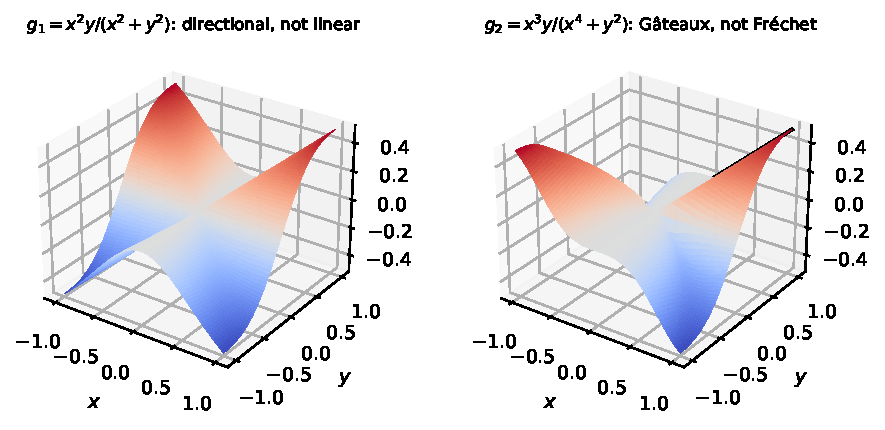
\includegraphics[width=\textwidth]{figures/appB/gateaux_frechet.pdf}
\caption{Left: $g_1$ has directional derivatives at the origin which are not
linear in the direction. Right: $g_2$ is G\^ateaux differentiable at the
origin (zero derivative along every straight line), but not Fr\'echet
differentiable: along the parabola $y=x^2$ (black curve) it grows like $x/2$.}
\label{fig:gateaux}
\end{figure}

%======================================================================
\section{Three equivalent problem settings}
\begin{gbox}{Problem settings}
\index{weak form}\index{strong form}\index{energy!minimization}%
\begin{description}[style=nextline,leftmargin=1em,font=\sffamily\bfseries]
\item[Energy minimization] Find $u_0$ minimizing $\mathcal W(u)$ over $V$.
\item[Weak formulation (virtual work)]
\[
  \delta\mathcal W(u_0)[v]=0\quad\forall v\in V,
  \qquad\text{or}\qquad
  \Bigl\langle\frac{\delta\mathcal W}{\delta u}(u_0),v\Bigr\rangle=0\quad\forall v\in V .
\]
\item[Strong formulation (Euler--Lagrange equations)]
\[
  \frac{\delta\mathcal W}{\delta u}(u_0)=0 .
\]
\end{description}
\end{gbox}
A minimizer satisfies the weak form (the first variation vanishes at a
minimum); for a convex $\mathcal W$ the converse holds. The difference between
the two weak forms lies in the derivatives of $v$: the first contains
derivatives of $v$, the second none, after integration by parts. Passing from
the weak to the strong form requires this integration by parts and enough
regularity of $u_0$.

%======================================================================
\section{Integral functionals and the Euler--Lagrange equations}
Let $\displaystyle \mathcal W(u)=\int_\Omega\mathcal F(\vx,u,\nabla u)\dd x$, with
$\mathcal F$ smooth. Differentiating under the integral,
\[
  \delta\mathcal W(u)[v]=\int_\Omega\Bigl(\frac{\partial\mathcal F}{\partial u}\,v
  +\frac{\partial\mathcal F}{\partial(\nabla u)}\cdot\nabla v\Bigr)\dd x .
\]
Integrating the second term by parts (Theorem~\ref{thm:ibp}):
\[
  \delta\mathcal W(u)[v]=\int_\Omega\Bigl(\frac{\partial\mathcal F}{\partial u}
  -\dive\frac{\partial\mathcal F}{\partial(\nabla u)}\Bigr)v\dd x
  +\int_{\partial\Omega}\frac{\partial\mathcal F}{\partial(\nabla u)}\cdot\vn\,v\dd s .
\]
\begin{gbox}{Euler--Lagrange equations}
\index{Euler--Lagrange equation}\index{boundary condition!natural}%
\begin{equation}\label{eq:EL}
  \frac{\delta\mathcal W}{\delta u}=\frac{\partial\mathcal F}{\partial u}
  -\dive\frac{\partial\mathcal F}{\partial(\nabla u)}=0\ \ \text{in }\Omega,
  \qquad
  \frac{\partial\mathcal F}{\partial(\nabla u)}\cdot\vn=0\ \ \text{where $u$ is not prescribed.}
\end{equation}
The boundary condition is \emph{natural}; where $u$ is prescribed, $v=0$ and
there is no condition.
\end{gbox}

\paragraph{General first-order operators.} More generally, let
\index{adjoint operator!formal}\index{beam!Euler--Bernoulli}%
$\displaystyle \mathcal W(u)=\int_\Omega\mathcal F(Du)\dd x$ with $D$ a linear differential
operator (components $D_i$). Then
\[
  \delta\mathcal W(u)[v]=\int_\Omega\frac{\partial\mathcal F}{\partial(D_iu)}\,D_iv\dd x=0
  \quad\forall v
  \qquad\Longleftrightarrow\qquad
  D_i^\ast\frac{\partial\mathcal F}{\partial(D_iu)}=0,
\]
where $D^\ast$ is the formal adjoint of $D$, defined by
$\displaystyle \int_\Omega(Du)\cdot w=\int_\Omega u\,D^\ast w$ for fields vanishing on the
boundary. The pairs used in this book are:
\begin{center}
\renewcommand{\arraystretch}{1.25}
\begin{tabular}{llll}
\toprule
\sffamily operator $D$ & \sffamily adjoint $D^\ast$ & \sffamily energy density & \sffamily Euler--Lagrange\\
\midrule
$\nabla$ (scalar) & $-\dive$ & $\tfrac12\nabla u\cdot\bbK\nabla u-fu$ & $-\dive(\bbK\nabla u)=f$\\
$\eps[\cdot]=\sym\nabla$ & $-\dive$ (on symmetric tensors) & $\tfrac12\eps:\bbC:\eps-\vf\cdot\vu$ & $-\dive(\bbC:\eps[\vu])=\vf$\\
$\dd/\dd x$ & $-\dd/\dd x$ & $\tfrac12EA(u')^2-fu$ & $-(EAu')'=f$\\
$\dd^2/\dd x^2$ & $\dd^2/\dd x^2$ & $\tfrac12EI(w'')^2-qw$ & $(EIw'')''=q$\\
$\mat{B}$ (matrix) & $\mat{B}\T$ & $\tfrac12\mat{B}\vu\cdot\mat{C}\mat{B}\vu-\vf\cdot\vu$ & $\mat{B}\T\mat{C}\mat{B}\vu=\vf$\\
\bottomrule
\end{tabular}
\end{center}
The last line is the spring chain of Section~\ref{sec:var-discrete}: the
adjoint of a differential operator is the continuum counterpart of the
transpose of a matrix.

%======================================================================
\section{Second variation and convexity}
\index{second variation}\index{convexity}%
The second G\^ateaux derivative,
$\displaystyle \delta^2\mathcal W(u)[v,w]=\frac{\partial^2}{\partial\alpha\,\partial\beta}\mathcal W(u+\alpha v+\beta w)\big|_{0}$,
is symmetric in $(v,w)$ when it exists and is continuous (Schwarz). This is
why a non-symmetric bilinear form cannot be the second variation of an energy
(Exercise~\ref{exo:no-energy}). If $\delta^2\mathcal W(u)[v,v]\ge0$ for all
$u,v$, $\mathcal W$ is convex and every critical point is a minimizer; if
$\delta^2\mathcal W(u)[v,v]\ge\alpha\norm{v}^2$, the minimizer is unique. A
critical point at which the second variation takes negative values is
unstable (the double well of Section~\ref{sec:var-lm}).

%======================================================================
\framepart{Summary}
\begin{gbox*}
\begin{itemize}
  \item The \textbf{G\^ateaux derivative} is the derivative along straight
  lines, $\displaystyle \frac{\dd}{\dd\alpha}\mathcal W(u_0+\alpha v)|_{\alpha=0}$; the
  \textbf{Fr\'echet derivative} is a uniform linear approximation. Fr\'echet
  implies G\^ateaux, not conversely.
  \item An energy problem has three settings: \textbf{minimization},
  \textbf{weak form} ($\delta\mathcal W(u)[v]=0$ for all $v$) and
  \textbf{strong form} ($\delta\mathcal W/\delta u=0$, the Euler--Lagrange
  equations, with natural boundary conditions).
  \item For $\displaystyle \mathcal W=\int\mathcal F(Du)$ the Euler--Lagrange operator is
  $D^\ast\,\partial\mathcal F/\partial(Du)$: the formal adjoint of a
  differential operator plays the role of the transpose of a matrix.
  \item The \textbf{second variation} is symmetric; its sign decides
  convexity, uniqueness and stability.
\end{itemize}
\end{gbox*}

\framepart{Exercises}

\exercise{A membrane, or steady heat conduction}\label{exo:A-membrane}
Find the three problem settings for
\[
  \mathcal W(u)=\int_\Omega\Bigl[\frac c2\Bigl(\frac{\partial u}{\partial x}\Bigr)^2
  +\frac c2\Bigl(\frac{\partial u}{\partial y}\Bigr)^2-fu\Bigr]\dd x\dd y,
  \qquad\Omega\subset\R^2 .
\]
Give a physical interpretation of the fields.
\begin{solution}
Minimization of $\mathcal W$ over $u$ (with $u$ given on part of the boundary).
Weak form: $\displaystyle \int_\Omega(c\nabla u\cdot\nabla v-fv)=0$ for all admissible $v$.
Strong form: $-c\Delta u=f$ in $\Omega$, $c\,\partial_nu=0$ where $u$ is free.
Interpretations: transverse deflection $u$ of a membrane of tension $c$ under
a pressure $f$; temperature $u$ in a plate of conductivity $c$ with heat
source $f$; Prandtl stress function of a twisted bar ($f=2\mu\theta$).
\end{solution}

\exercise{From the strong form back to the energy}\label{exo:A-pendulum}
The strong formulation of a problem is $-u''+\sin u=0$,
$u:\R\to\R$. Find its weak formulation and its energy functional.
\begin{solution}
Weak form: $\displaystyle \int(u'v'+\sin u\,v)\dd x=0$ for all $v$ with compact support.
Since $\displaystyle \sin u=\frac{\dd}{\dd u}(-\cos u)$, the energy is
$\displaystyle \mathcal W(u)=\int\bigl(\tfrac12(u')^2-\cos u\bigr)\dd x$ (up to a constant).
With $x$ read as time it is the action of a pendulum,
$\displaystyle \int(\text{kinetic}-\text{potential})$ with potential $\cos u$, i.e.\ an inverted
pendulum; it is also the static sine-Gordon equation for a chain of torsion
springs. The energy is not convex: $\displaystyle \delta^2\mathcal W(u)[v,v]=\int((v')^2+\cos u\,v^2)$
can be negative.
\end{solution}

\exercise{Minimal surfaces}\label{exo:A-minimal}
Find the three problem settings for
\[
  \mathcal W(u)=\int_\Omega\Bigl[1+\Bigl(\frac{\partial u}{\partial x}\Bigr)^2
  +\Bigl(\frac{\partial u}{\partial y}\Bigr)^2\Bigr]^{1/2}\dd x\dd y,
  \qquad u=u_0\ \text{on }\partial\Omega .
\]
Give a physical interpretation. Hint:
$\displaystyle (1+a+b)^{1/2}=(1+a)^{1/2}+\frac{b}{2(1+a)^{1/2}}+O(b^2)$.
\begin{solution}
$\mathcal W$ is the area of the graph of $u$. With
$a=|\nabla u|^2$ and $b=2\alpha\nabla u\cdot\nabla v+\alpha^2|\nabla v|^2$, the hint
gives
$\displaystyle \delta\mathcal W(u)[v]=\int_\Omega\frac{\nabla u\cdot\nabla v}{\sqrt{1+|\nabla u|^2}}=0$
for all $v$ vanishing on $\partial\Omega$ (weak form), and
$\dive\bigl(\nabla u/\sqrt{1+|\nabla u|^2}\bigr)=0$ (strong form, the minimal
surface equation). The left-hand side is twice the mean curvature of the
graph: a soap film spanning the wire $u_0$ has zero mean curvature
(Section~\ref{sec:var-phys}). For small slopes, $\displaystyle \mathcal W\approx|\Omega|+\tfrac12\int|\nabla u|^2$
and the equation linearizes to $\Delta u=0$.
\end{solution}

\exercise{Derivative of the elastic energy}\label{exo:A-elastic}
Compute the G\^ateaux derivative of
$\displaystyle \mathcal U(\vu)=\int_\Omega\tfrac12\eps[\vu]:\bbC:\eps[\vu]\dd x$ and show that
it is a Fr\'echet derivative on $H^1(\Omega)^3$.
\begin{solution}
$\displaystyle \mathcal U(\vu+\alpha\vv)=\mathcal U(\vu)+\alpha\int\eps[\vu]:\bbC:\eps[\vv]+\alpha^2\mathcal U(\vv)$
by the major symmetry of $\bbC$, so
$\displaystyle \delta\mathcal U(\vu)[\vv]=\int_\Omega\eps[\vu]:\bbC:\eps[\vv]$, linear and bounded
in $\vv$. The remainder is $\mathcal U(\vv)\le\tfrac12|\bbC|\,\norm{\vv}_{H^1}^2=o(\norm{\vv})$:
the derivative is Fr\'echet.
\end{solution}

%======================================================================
\begin{chapterbib}{9}
\bibitem{DacorognaIntro} B.~Dacorogna, \emph{Introduction to the Calculus of Variations}, 3rd ed., Imperial College Press, 2015.
\bibitem{GelfandFomin} I.~M.~Gelfand, S.~V.~Fomin, \emph{Calculus of Variations}, Prentice-Hall, 1963 (Dover reprint, 2000).
\end{chapterbib}

%======================================================================
\chapter[Integration by parts: the Gauss--Ostrogradsky family]{Integration by parts:\\ the Gauss--Ostrogradsky family}\label{app:ibp}
%======================================================================
% Sources: "Why variational formulations matter", Section 11; notes C1.

\framepart{Outline}
Every weak formulation and every adjoint computation in this book rests on a
small family of classical identities. Throughout, $\Omega\subset\R^3$ is a
bounded domain with Lipschitz boundary $\partial\Omega$, outward unit normal
$\vn$ and surface measure $\dd s$~\cite{MarsdenTromba2011,Evans2010B}. Indices
refer to Cartesian components, with summation over repeated indices and
$(\cdot)_{,j}=\partial(\cdot)/\partial x_j$.

%======================================================================
\section{The divergence theorem}
\begin{theorem}[Gauss--Ostrogradsky]\label{thm:div}
\index{divergence theorem}\index{Gauss--Ostrogradsky theorem}\index{Stokes theorem}%
For a vector field $\vF\in C^1(\overline\Omega;\R^3)$,
\[
  \int_\Omega\dive\vF\dd x=\int_{\partial\Omega}\vF\cdot\vn\dd s,
  \qquad\text{i.e.}\qquad
  \int_\Omega F_{i,i}\dd x=\int_{\partial\Omega}F_in_i\dd s .
\]
\end{theorem}
This is the master identity; every formula below follows from it and a
product rule. By density it extends to Sobolev fields, with boundary values
understood as traces.\footnote{On the names: the divergence theorem is due to
Gauss (1813, a special case) and Ostrogradsky (1826, the general proof),
independently of the curl theorem now called after Stokes. That theorem was
itself communicated by Kelvin to Stokes in a letter of 2 July 1850 and owes
its name to a question Stokes set in the 1854 Smith's Prize
examination~\cite{Katz1979}, hence the name Kelvin--Stokes. All of these are
special cases of the generalized Stokes theorem for differential forms,
$\displaystyle \int_Md\omega=\int_{\partial M}\omega$, which is why the divergence theorem
is sometimes called ``Stokes' theorem'' too. We stay with classical vector
calculus and keep the names separate, following~\cite{MarsdenTromba2011}.}

%======================================================================
\section{Scalar fields}
\begin{theorem}[Integration by parts, scalar times vector]\label{thm:ibp}
\index{integration by parts!scalar field}%
For $u\in C^1(\overline\Omega)$ and $\vF\in C^1(\overline\Omega;\R^3)$,
applying Theorem~\ref{thm:div} to $\dive(u\vF)=u\dive\vF+\nabla u\cdot\vF$,
\[
  \int_\Omega u\dive\vF\dd x=-\int_\Omega\nabla u\cdot\vF\dd x
  +\int_{\partial\Omega}u\,(\vF\cdot\vn)\dd s .
\]
\end{theorem}
With $\vF=\nabla u/\sqrt{1+|\nabla u|^2}$ it gives the minimal surface
equation (Section~\ref{sec:var-phys}); with $\vF=\vp$ the adjoint
$\Lambda^\ast\vp=-\dive\vp$ of Section~\ref{sec:var-dual}.

\begin{corollary}[Componentwise]\label{cor:comp}
\index{integration by parts!componentwise}%
For $i=1,2,3$ and $u,v\in C^1(\overline\Omega)$,
$\displaystyle\int_\Omega u\,v_{,i}\dd x=-\int_\Omega u_{,i}\,v\dd x+\int_{\partial\Omega}uv\,n_i\dd s$.
\end{corollary}

\begin{theorem}[Green's first identity]\label{thm:green1}
\index{Green's identities!first}%
Taking $\vF=\nabla v$ in Theorem~\ref{thm:ibp},
\[
  \int_\Omega\nabla u\cdot\nabla v\dd x=-\int_\Omega u\,\Delta v\dd x
  +\int_{\partial\Omega}u\,\partial_nv\dd s .
\]
\end{theorem}
This is the identity that passes from the strong to the weak form of
$-\Delta u=f$ (Section~\ref{sec:var-weak}).

\begin{theorem}[Green's second identity]\label{thm:green2}
\index{Green's identities!second}%
Subtracting Theorem~\ref{thm:green1} from itself with $u$ and $v$ exchanged,
\[
  \int_\Omega\bigl(u\,\Delta v-v\,\Delta u\bigr)\dd x
  =\int_{\partial\Omega}\bigl(u\,\partial_nv-v\,\partial_nu\bigr)\dd s .
\]
\end{theorem}
This symmetric form makes the Laplacian self-adjoint
(Exercise~\ref{exo:selfadj}). It is the continuum form of the reciprocity
theorem (Section~\ref{ssec:reciprocity}) and the starting point of the
reciprocity gap (Chapter~\ref{ch:rg}).

\begin{theorem}[Matrix coefficient field]\label{thm:ibp-matrix}
\index{integration by parts!matrix coefficient}%
For a second-order tensor field $\tA\in C^1(\overline\Omega;\R^{3\times3})$ and
$u,v\in C^1(\overline\Omega)$, Theorem~\ref{thm:ibp} with $\vF=\tA\nabla u$ gives
\[
  \int_\Omega\tA\nabla u\cdot\nabla v\dd x
  =-\int_\Omega\dive(\tA\nabla u)\,v\dd x+\int_{\partial\Omega}v\,(\tA\nabla u)\cdot\vn\dd s .
\]
If $\tA$ is symmetric, exchanging $u$ and $v$ and subtracting gives the
second identity
$\displaystyle \int_\Omega\bigl(u\dive(\tA\nabla v)-v\dive(\tA\nabla u)\bigr)
=\int_{\partial\Omega}\bigl(u\,(\tA\nabla v)\cdot\vn-v\,(\tA\nabla u)\cdot\vn\bigr)$.
\end{theorem}
It is used for the general elliptic operator (Section~\ref{sec:var-elliptic})
and for the diffusion problem (Section~\ref{sec:diff}).

%======================================================================
\section{Tensor fields}
For a second-order tensor field $\sig$, the divergence is the vector
$(\dive\sig)_i=\sigma_{ij,j}$, and $\sig\vn$ has components $\sigma_{ij}n_j$.

\begin{theorem}[Tensor times vector]\label{thm:ibp-tensor}
\index{integration by parts!tensor field}\index{reciprocity!Betti (elasticity)}%
For $\sig\in C^1(\overline\Omega;\R^{3\times3})$ and
$\vv\in C^1(\overline\Omega;\R^3)$,
\[
  \int_\Omega\sig:\nabla\vv\dd x=-\int_\Omega(\dive\sig)\cdot\vv\dd x
  +\int_{\partial\Omega}(\sig\vn)\cdot\vv\dd s .
\]
If $\sig$ is symmetric, $\sig:\nabla\vv=\sig:\eps[\vv]$ with
$\eps[\vv]=\tfrac12(\nabla\vv+\nabla\vv\T)$.
\end{theorem}
\begin{proof}
Apply Theorem~\ref{thm:div} to the vector $F_j=\sigma_{ij}v_i$:
$F_{j,j}=\sigma_{ij,j}v_i+\sigma_{ij}v_{i,j}$ and $F_jn_j=(\sigma_{ij}n_j)v_i$.
For symmetric $\sig$, the antisymmetric part of $\nabla\vv$ does not
contribute to $\sig:\nabla\vv$.
\end{proof}
This identity gives the principle of virtual work (Section~\ref{sec:el-vw}):
the divergence on symmetric tensors is minus the adjoint of the symmetric
gradient. With $\sig=\bbC:\eps[\vu]$ and $\bbC$ having the major symmetry, it
gives the Betti reciprocity theorem of elasticity,
\[
  \int_\Omega\bigl(\vu\cdot\dive\sig[\vv]-\vv\cdot\dive\sig[\vu]\bigr)\dd x
  =\int_{\partial\Omega}\bigl(\vu\cdot\sig[\vv]\vn-\vv\cdot\sig[\vu]\vn\bigr)\dd s .
\]

%======================================================================
\section{Domains with a cut}
\index{integration by parts!cracked domain}\index{jump}%
When $\Omega$ contains a crack $\Gamma$ with lips $\Gamma^\pm$, the identities
hold in $\OG=\Omega\setminus\Gamma$, whose boundary consists of $\partial\Omega$,
with outward normal $\vnu$, and of both lips (Figure~\ref{fig:lips}). If $\vn$
is the normal of $\Gamma$ pointing towards $\Gamma^+$, the outward normal of
$\OG$ is $-\vn$ on $\Gamma^+$ and $+\vn$ on $\Gamma^-$. For a field $\vF$ smooth
on each side,
\[
  \int_{\OG}\dive\vF\dd x=\int_{\partial\Omega}\vF\cdot\vnu\dd s
  -\int_\Gamma\jump{\vF}\cdot\vn\dd s,\qquad\jump{\vF}=\vF^+-\vF^- .
\]
\begin{figure}[h]
\centering
\begin{tikzpicture}[scale=1.05,>=Stealth]
  \fill[gray!8] plot[smooth cycle,tension=0.8] coordinates{(-3,0) (-2,1.8) (0.5,2.1) (3,1.2) (3.2,-1) (1,-2) (-2,-1.6)};
  \draw[thick] plot[smooth cycle,tension=0.8] coordinates{(-3,0) (-2,1.8) (0.5,2.1) (3,1.2) (3.2,-1) (1,-2) (-2,-1.6)};
  \node at (-2.2,0.9) {$\OG$};
  \node at (2.75,1.75) {$\partial\Omega$};
  \draw[->,thick] (3.12,0.2) -- (3.9,0.32) node[right] {$\vnu$};
  % crack drawn slightly open
  \draw[line width=1.2pt,cu] (-1.2,0.07) .. controls (0,0.12) .. (1.2,0.07);
  \draw[line width=1.2pt,cphi] (-1.2,-0.07) .. controls (0,-0.12) .. (1.2,-0.07);
  \fill[white] (-1.2,0.07) -- (1.2,0.07) -- (1.2,-0.07) -- (-1.2,-0.07) -- cycle;
  \draw[line width=1.2pt,cu] (-1.2,0.07) .. controls (0,0.12) .. (1.2,0.07);
  \draw[line width=1.2pt,cphi] (-1.2,-0.07) .. controls (0,-0.12) .. (1.2,-0.07);
  \node[cu] at (-1.55,0.35) {$\Gamma^+$};
  \node[cphi] at (-1.55,-0.38) {$\Gamma^-$};
  % normal of the crack
  \draw[->,very thick] (1.65,0) -- (1.65,0.75) node[right] {$\vn$};
  \draw[dashed,gray] (1.2,0) -- (1.65,0);
  % outward normals of Omega_Gamma on the lips
  \draw[->,thick,cu] (0,0.65) -- (0,0.16);
  \node[cu,right] at (0,0.5) {\small $-\vn$};
  \draw[->,thick,cphi] (0,-0.65) -- (0,-0.16);
  \node[cphi,right] at (0,-0.5) {\small $+\vn$};
\end{tikzpicture}
\caption{A body $\Omega$ cut by a crack $\Gamma$ (drawn open). The crack
normal $\vn$ points towards the upper lip $\Gamma^+$. The outward normal of
the cut domain $\OG$ is $\vnu$ on $\partial\Omega$, $-\vn$ on $\Gamma^+$ and
$+\vn$ on $\Gamma^-$: the two lips are seen from opposite sides, which is the
origin of the jump $\jump{\vF}=\vF^+-\vF^-$ and of most sign errors.}
\label{fig:lips}
\end{figure}
This is how the jump of the potential across the crack appears in the
reciprocity gap identity~\eqref{eq:rg-rg}.

%======================================================================
\framepart{Summary}
All the identities follow from the divergence theorem and a product rule.
The table lists where each one is used in the book.
\begin{center}
\renewcommand{\arraystretch}{1.15}
\begin{tabular}{ll}
\toprule
\sffamily where used & \sffamily identity\\
\midrule
weak form of $-\Delta u=f$ (Section~\ref{sec:var-weak}) & Green's first identity, Theorem~\ref{thm:green1}\\
symmetry of $a(u,v)$, reciprocity (Sections~\ref{sec:var-lm}, \ref{ssec:reciprocity}) & Green's second identity, Theorem~\ref{thm:green2}\\
minimal surface equation (Section~\ref{sec:var-phys}) & Theorem~\ref{thm:ibp}\\
general elliptic operator, diffusion (Sections~\ref{sec:var-elliptic}, \ref{sec:diff}) & Theorem~\ref{thm:ibp-matrix}\\
dual problem, $\Lambda^\ast=-\dive$ (Section~\ref{sec:var-dual}) & Theorem~\ref{thm:ibp}\\
virtual work, Navier equations (Sections~\ref{sec:el-vw}, \ref{sec:el-energy}) & Theorem~\ref{thm:ibp-tensor}\\
reciprocity gap (Section~\ref{sec:rg-gap}) & Green's second identity in $\OG$\\
\bottomrule
\end{tabular}
\end{center}

\paragraph{The classical trio.} The divergence theorem is the
three-dimensional member of a family that also contains the \emph{gradient
theorem} (fundamental theorem of line integrals) and \emph{Stokes' theorem}
(the flux of $\operatorname{curl}\vF$ through a surface equals the
circulation of $\vF$ along its boundary curve). Together they generalize the
fundamental theorem of calculus to higher dimensions~\cite{MarsdenTromba2011}.
Only the divergence theorem is needed here, since every variational problem
of the book is built from $\nabla$ and its adjoint $-\dive$.

%======================================================================
\begin{chapterbib}{9}
\bibitem{Evans2010B} L.~C.~Evans, \emph{Partial Differential Equations}, 2nd ed., AMS, 2010.
\bibitem{Katz1979} V.~J.~Katz, The history of Stokes' theorem, \emph{Math. Mag.} 52 (1979) 146--156.
\bibitem{MarsdenTromba2011} J.~E.~Marsden, A.~J.~Tromba, \emph{Vector Calculus}, 6th ed., W.~H.~Freeman, 2011.
\end{chapterbib}


\backmatter
\printindex

\end{document}
